% $Header$
% MBDyn (C) is a multibody analysis code.
% http://www.mbdyn.org
%
% Copyright (C) 1996-2010
%
% Pierangelo Masarati  <masarati@aero.polimi.it>
%
% Dipartimento di Ingegneria Aerospaziale - Politecnico di Milano
% via La Masa, 34 - 20156 Milano, Italy
% http://www.aero.polimi.it
%
% Changing this copyright notice is forbidden.
%
% This program is free software; you can redistribute it and/or modify
% it under the terms of the GNU General Public License as published by
% the Free Software Foundation (version 2 of the License).
% 
%
% This program is distributed in the hope that it will be useful,
% but WITHOUT ANY WARRANTY; without even the implied warranty of
% MERCHANTABILITY or FITNESS FOR A PARTICULAR PURPOSE.  See the
% GNU General Public License for more details.
%
% You should have received a copy of the GNU General Public License
% along with this program; if not, write to the Free Software
% Foundation, Inc., 59 Temple Place, Suite 330, Boston, MA  02111-1307  USA

\documentclass[10pt,dvips,fleqn,subeqn]{report}

%\usepackage[pdftex]{graphicx}
\usepackage[T1]{fontenc}
\usepackage{ae,aecompl}
\usepackage{graphicx}
\usepackage{psfrag}
\usepackage{bm, amsmath, amsfonts, amssymb}
%\usepackage[dvips,breaklinks=true,colorlinks=false]{hyperref}
\usepackage{html}
\usepackage{comment}

% $Header$
% Copyright (C) 1996-2013 Pierangelo Masarati <masarati@aero.polimi.it>
% Dipartimento di Ingegneria Aerospaziale, Politecnico di Milano
%
% Parentesi: tonde, quadre, curly, dritte, doppie e angolari.
\newcommand{\plbr}[1]{ \left( #1 \right) }
\newcommand{\sqbr}[1]{ \left[ #1 \right] }
\newcommand{\cubr}[1]{ \left\{ #1 \right\} }
\newcommand{\shbr}[1]{ \left| #1 \right| }
\newcommand{\nrbr}[1]{ \left\| #1 \right\| }
\newcommand{\anbr}[1]{ \langle #1 \rangle }

% Parentesi solo a sinistra: tonde, quadre, curly, dritte, doppie e angolari.
\newcommand{\lplbr}[1]{ \left( #1 \right. }
\newcommand{\lsqbr}[1]{ \left[ #1 \right. }
\newcommand{\lcubr}[1]{ \left\{ #1 \right. }
\newcommand{\lshbr}[1]{ \left| #1 \right. }
\newcommand{\lnrbr}[1]{ \left\| #1 \right. }
\newcommand{\lanbr}[1]{ \langle #1 \right. }

% Parentesi solo a destra: tonde, quadre, curly, dritte,doppie e angolari.
\newcommand{\rplbr}[1]{ \left. #1 \right) }
\newcommand{\rsqbr}[1]{ \left. #1 \right] }
\newcommand{\rcubr}[1]{ \left. #1 \right\} }
\newcommand{\rshbr}[1]{ \left. #1 \right| }
\newcommand{\rnrbr}[1]{ \left. #1 \right\| }
\newcommand{\ranbr}[1]{ \left. #1 \rangle }

% Vettori verticali:
\newcommand{\vvect}[2]{ \begin{array}{ #1 } #2 \end{array} }
\newcommand{\cvvect}[1]{ \begin{array}{c} #1 \end{array} }
\newcommand{\lvvect}[1]{ \begin{array}{l} #1 \end{array} }
\newcommand{\rvvect}[1]{ \begin{array}{r} #1 \end{array} }

% Vettori orizzontali:
\newcommand{\hvect}[2]{ \begin{array}{ #1 } #2 \end{array} }

% Matrici:
\newcommand{\matr}[2]{ \begin{array}{ #1 } #2 \end{array} }

% Integrali: uso \intg{inf}{sup}{arg}{dvar}
\newcommand{\intg}[4]{ \int_{#1}^{#2} {#3} \ {#4} }

% Limite: uso \limt{var}{lim}{arg}
\newcommand{\limt}[3]{ \lim_{{#1} \rightarrow {#2}} {#3}}

% LogLike functions
\newcommand{\llk}[1]{\ensuremath{\mathrm{#1}}}

\newcommand{\diag}[0]{\llk{diag}}
\newcommand{\tr}[0]{\llk{tr}}
\newcommand{\sym}[0]{\llk{sym}}
\newcommand{\skw}[0]{\llk{skw}}

\newcommand{\step}[0]{\llk{step}}
\newcommand{\imp}[0]{\llk{imp}}

\newcommand{\grad}[0]{\llk{grad}}
\newcommand{\divr}[0]{\llk{div}}
\newcommand{\rot}[0]{\llk{rot}}

% In italiano ...
\newcommand{\sca}[0]{\llk{sca}}

% first, second, etc
\newcommand{\first}[0]{1\ensuremath{^{\mathrm{st}}}}    % 1^st
\newcommand{\second}[0]{2\ensuremath{^{\mathrm{nd}}}}   % 2^nd
\newcommand{\third}[0]{3\ensuremath{^{\mathrm{rd}}}}    % 3^rd
\newcommand{\rth}[0]{\ensuremath{^{\mathrm{th}}}}       %  ^th

\newcommand{\degr}[0]{\ensuremath{^{\mathrm{o}}}}

% esponenziale
\providecommand{\e}[1]{\llk{e}^{#1}}

%poor man's bold symbol
\newcommand{\T}[1]{\bm{\mathbf{#1}}}
\newcommand{\TT}[1]{\bm{\mathbf{#1}}}
\newcommand{\TTT}[1]{\bm{\mathbf{#1}}}
\newcommand{\TTTT}[1]{\mathbb{#1}}
\newcommand{\equu}{\overset{\text{uu}}{=}}
\newcommand{\dof}{DOF}
\newcommand{\dofs}{DOFs}

% Custom
\topmargin 0.31cm % 0.00cm
\oddsidemargin 0.00cm
\evensidemargin 0.00cm
\marginparsep 0.00cm
\textwidth 15.92cm
\textheight 21.00cm % 23.62cm

\begin{document}

\begin{latexonly}
\title{\bf MBDyn Theory \\ and Developer's Manual \\
Version
0.1.0

}
\author{Pierangelo Masarati \vspace{5mm}\\
    \sc Dipartimento di Ingegneria Aerospaziale \\
    \sc Politecnico di Milano}
\date{\today}
\maketitle
\end{latexonly}

\begin{htmlonly}
\begin{center}
\textbf{\LARGE MBDyn Technical Manual}

\emph{\large Pierangelo Masarati}

\textsc{Dipartimento di Ingegneria Aerospaziale \\ Politecnico di Milano}

\today
\end{center}
\end{htmlonly}




\tableofcontents
\newpage
\listoffigures
\newpage
\listoftables
\newpage



\chapter{Introduction}
This document describes the formulation MBDyn,
the free general-purpose multibody dynamics software,
relies on.
It also describes implementation-related aspects.

The document is far from complete; in fact, its preparation
started at a late stage of the project, when many parts
of the software were already completed and in use.
From that time on, many modifications and improvements
have been steadily documented and, occasionally,
the theory manual anticipated the development
(as should always happen, I know).

The Developers committed themselves to keeping it at least up to date
with new developments; undocumented stuff should be documented
as soon as it needs modifications or refactoring.

Alessandro Fumagalli and Marco Morandini contributed significantly
to this document.



\chapter{Parsing}
In MBDyn there are different levels of parsing.
Input file parsing suffers from a scattered and occasionally outdated design.
The need to preserver backwards compatibility with existing models
restrains from entirely redesign it, although selected improvements
occur over time.

MBDyn provides support for the implementation of new functionalities,
and to parse their input.
Parsing is delegated to a dedicated object, the MBDynParser, which
inherits from the HighParser, a higher-level parsing object 
with bits of MBDyn's syntax built-in in a somewhat modular way.
It exploits the functionalities of the LowParser, a lower-level
parsing object that deals with tokenizing an input stream
based on the expected tokens.
Whenever appropriate (e.g.\ whenever a number is expected),
control is delegated to the MathParser, which allows to parse and evaluate
sequences of mathematical expressions, including variable declaration
and definition.
Variables are saved in a table as soon as they appear, and can be
used by subsequent expressions when the mathematical parser is called again.

The traditional approach to data parsing consists in defining a table
of keywords that are looked up and, based on the corresponding key code,
by executing the appropriate code in a switch-case block.

The code is being gradually moved to a newer approach based on sets
of associative arrays that map keywords to the functional objects
that are used to parse the related items.

Although no significant improvement results in parsing of existing 
data types, this approach allows to register new data types run-time,
e.g.\ from a run-time loaded module, thus easing the extension
and the customization of the code.


\section{HighParser}
\subsection{Traditional Usage}
The \texttt{HighParser} class and its descendants use a \texttt{KeyTable}
object containing a list of legal keywords to return a valid keyword index
when \texttt{HighParser::GetWord()}, and significantly 
\texttt{HighParser::GetDescription()} are invoked.
The \texttt{KeyTable} can be changed during parsing.
\texttt{KeyTable} is a class.
Its constructor takes a pointer to an array of strings and a reference 
to the \texttt{HighParser} object.
The last string in the array must be null.
The \texttt{KeyTable} class constructor keeps track 
of previous \texttt{KeyTable} objects in the \texttt{HighParser}, 
and restores them upon destruction.

The suggested usage inside a stacked call sequence of parsing functions is
\begin{verbatim}
Part *
read_part(HighParser& HP)
{
    /* prepare names */
    enum KeyWord { KEYWORD1, KEYWORD2, KEYWORD_LAST };
    char *key_table_array[] = { "keyword1", "keyword2", 0 };
    /* build KeyTable class */
    KeyTable k(HP, key_table_array);
    Part *returned_object = 0;
    /* parse input */
    do {
        switch (KeyWord(HP.GetWord())) {
        default:
            /* do something... */
            break;
        case KEYWORD1:
            /* ...and build returned_object  */
            return returned_object;
        }
    } while (true);
}

void
read_all(HighParser& HP)
{
    /* prepare names */
    enum KeyWord { KEY1, KEY2, PART, KEY_LAST };
    char *keytable[] = { "key1", "key2", "part", 0 };
    /* build KeyTable class */
    KeyTable k(HP, keytable);
    /* do something */
    Part *part = 0;
    do {
        switch (KeyWord(HP.GetWord())) {
        default:
            /* do something... */
            break;
        case PART:
            /* read part */
            Part *part = read_part(HP);
            break;
        }
    } while (true);
}

\end{verbatim}
Here the \texttt{KeyTable} set by function \texttt{read\_all()} 
is automatically restored after the call to \texttt{read\_part()}; 
\texttt{read\_part()} temporarily changes the \texttt{KeyTable}
used by the parser.

\subsection{Table-Driven Usage}
The table-driven usage is based on defining a functional object 
that is able to parse a data type:
\begin{verbatim}
    class Datum {
    public:
        virtual ~Datum(void) {};
    };

    struct DatumRead {
        virtual ~DatumRead(void) {};
        virtual Datum *Read(MBDynParser &HP) const = 0;
    };
\end{verbatim}
and a container for its descendants:
\begin{verbatim}
    typedef std::string KeyType;
    typedef std::map<KeyType, DatumRead *> DatumMapType;
    DatumMapType DatumMap;
\end{verbatim}
Then, a functional object for each specific datum type is derived from
\texttt{DatumRead} \ldots
\begin{verbatim}
    class MyDatum : public Datum {
        // ...
    public:
        Datum(int);
        // ...
    }

    struct MyDatumRead : public DatumRead {
        Datum *Read(MBDynParser &HP) const {
            return new MyDatum(HP.GetInt());
        };
    };
\end{verbatim}
\ldots and stored exactly once into the associative container by means
of a dedicated helper:
\begin{verbatim}
    bool
    SetDatumRead(KeyType key, DatumRead *rf)
    {
        return DatumMap.insert(DatumMapType::value_type(key, rf)).second;
    }

    // somewhere early in the code ...
    SetDatumRead("mydatum", new MyDatumRead);

    // note: somewhere else later, in the code, place
    for (DatumMapType::iterator i = DatumMap.begin();
        i != DatumMap.end();
        i++)
    {
        delete i->second;
    }
\end{verbatim}
The parsing function is something like
\begin{verbatim}
    Datum *
    ReadDatum(MBDynParser &HP)
    {
        KeyType key(HP.GetStringWithDelims());
        if (key.c_str() == 0) {
            // error ...
            return 0;
        }
        DatumMapType::iterator i = DatumMap.find(key);
        if (i == DatumMap.end()) {
            // error ...
            return 0;
        }
        return i->second->Read(HP);
    }
\end{verbatim}
Only the \texttt{MyDatum} portions need be added for each new datum type;
they can be declared, defined and registered anywhere in the code,
including in run-time loaded modules.

Currently, drives, constitutive laws and scalar functions are handled
according to this scheme; examples are provided
in \texttt{modules/module-drive/},
\texttt{modules/module-constlaw/}
and
\texttt{modules/module-scalarfunc/}.
More types will be reworked accordingly.



\section{LowParser}
... 

\section{MathParser}
...

\chapter{Solvers}
...
\section{Matrix classes}

\section{Sparse matrices}

\section{Linear solvers}
LinearSolver classes wraps linear solvers\\
SolutionManagers classes deals with the solution of linear systems.
They own a pointer to a LinearSolver, where they allocate
the underlying linear solver.
SolutionManager::MatrInitialize() is called
when the structure of the underlying spares matrix changes.
SolutionManager::MatrReset(), is called to delete a factorization.
It usually calls LinearSolver::Reset(). The matrix has to be explicitly
zeroed before a Jacobian matrix assembly.

\section{Non linear solvers}
...
\section{Parallel solver}
\subsection{Partitioning}
\texttt{iTotVertices} is equal to the sum of nodes and elements. 
It is made in this way because we want the partitioner 
to generate a twofold subdivision:
\begin{itemize}
\item a subdivision related to elements; 
this subdivision is done in order to share the computational 
load during the assembly phase;
\item a subdivision related to nodes, 
which is necessary for the solving phase with the substructuring method.
\end{itemize}
Of course this two partitions must be connected, 
so we build created a graph which is made of nodes and elements as vertex. 
The connection between vertexes are only between nodes and elements. 
There is no node to node or element to element connection.

\texttt{pVertexWgts} 
contains what we call the computational weight of each entity, 
so nodes have weight null while elements has a weight related to 
the dimension of the submatrix of the Jacobian matrix assembled
by each one of them.

\texttt{pCommWgts} contains the communication weights 
(see metis documentation) which are a measure of the quantity 
of data which needs to be sent if the i-th vertex is part 
of an interface between different partitions. 
This means that nodes have a \texttt{CommWgts} equal to the number 
of \dofs, while elements have a weight equal
to any internal \dofs\ they possess.


\chapter{Orientation Handling}
The orientation of structural nodes is handled by storing the orientation
matrix of each node, and updating it during prediction and correction 
by incremental orientations.

The code uses Gibbs-Rodrigues parameters to account for incremental 
rotations.
These parameters allow very efficient implementation, since they
only require few algebraic operations to obtain the orientation matrix
and related entities.
However, they require the absolute value of the orientation to be limited;
this requirement is usually overcome by accuracy requirements,
so it is not viewed as a strong limitation.

One main advantage of this approach is that only three parameters
are required to handle orientations.
A main drawback of this approach is that it is quite difficult
to keep track of how large a change in orientation occurred
to a given node, since simply converting the orientation matrix 
into any other representation of a finite rotation typically results
in the minimal rotation that yields that matrix.

MBDyn can output rotations in the following representations:
\begin{itemize}
\item Euler angles according to the 123 sequence;
\item the orientation vector;
\item the orientation matrix.
\end{itemize}

\section{Euler Angles}
Consider an orientation expressed by matrix $\T{R}$.
It can be expressed as the result of a precise sequence of rotations 
about three distinct axes.
The 123 sequence means that matrix $\T{R}$ is obtained as a sequence
of three rotations: the first about axis 1; the second about axis 2
as it results after the first rotation; the third about axis 3
as it results after the second rotation, namely:
\begin{equation}
	\T{R}_1 = \sqbr{\matr{ccc}{
		1 & 0 & 0 \\
		0 & \cos\alpha & -\sin\alpha \\
		0 & \sin\alpha & \cos\alpha
	}} ,
\end{equation}
\begin{equation}
	\T{R}_2 = \sqbr{\matr{ccc}{
		\cos\beta & 0 & \sin\beta \\
		0 & 1 & 0 \\
		-\sin\beta & 0 & \cos\beta
	}} ,
\end{equation}
\begin{equation}
	\T{R}_3 = \sqbr{\matr{ccc}{
		\cos\gamma & -\sin\gamma & 0 \\
		\sin\gamma & \cos\gamma & 0 \\
		0 & 0 & 1
	}} ,
\end{equation}
piled up, must equal $\T{R}$:
\begin{align}
	\T{R} &= \T{R}_1 \T{R}_2 \T{R}_3 \\
	&= \sqbr{\matr{ccc}{
		\cos\beta \cos\gamma
		& -\cos\beta \sin\gamma
		& \sin\beta \\
		\sin\alpha \sin\beta \cos\gamma + \cos\alpha \sin\gamma
		& -\sin\alpha \sin\beta \sin\gamma + \cos\alpha \cos\gamma
		& -\sin\alpha \cos\beta \\
		-\cos\alpha \sin\beta \cos\gamma + \sin\alpha \sin\gamma
		& \cos\alpha \sin\beta \sin\gamma + \sin\alpha \cos\gamma
		& \cos\alpha \cos\beta
	}} \nonumber .
\end{align}
The angles can then be computed by means of a simple, 
partially recursive algorithm:
\begin{align}
	\alpha &= - \tan^{-1}\plbr{\cfrac{\T{R}_{23}}{\T{R}_{33}}} \\
	\beta &= \tan^{-1}\plbr{\cfrac{\T{R}_{13}}{
			\cos\alpha \T{R}_{33} - \sin\alpha \T{R}_{23}
		}} \\
	\gamma &= \tan^{-1}\plbr{\cfrac{
		\cos\alpha \T{R}_{21} + \sin\alpha \T{R}_{31}
	}{
		\cos\alpha \T{R}_{22} + \sin\alpha \T{R}_{32}
	}}
\end{align}
The use of the function \texttt{atan2(double dSin, double dCos)}
eliminates the risk of divisions by zero or of excessive loss of precision.



\section{Orientation Vector}
An orientation matrix can be represented as a finite rotation about 
an axis, in the form
\begin{equation}
	\T{R} = \T{I}
	+ \sin\phi \ \T{n}\times{}
	+ \plbr{1 - \cos\phi} \T{n}\times\T{n}\times{}
\end{equation}
where $\phi$ is the amplitude of the rotation and $\T{n}$ 
is the unit vector that represents the rotation axis.

Simple algebra manipulation shows that the trace of the orientation matrix
corresponds to 
\begin{align}
	\mathrm{tr}\plbr{\T{R}}
	&= \mathrm{tr}\plbr{\T{I}}
	+ \plbr{1 - \cos\phi}\mathrm{tr}\plbr{\T{n}\times\T{n}\times{}} \\
	&= 3 - 2 \plbr{1 - \cos\phi} ,
\end{align}
since
\begin{equation}
	\T{n}\times\T{n}\times{} = \T{n} \T{n}^T - \T{I} ,
\end{equation}
so
\begin{equation}
	\cos\phi = \frac{\mathrm{tr}\plbr{\T{R}} - 1}{2} .
\end{equation}

At the same time, the skew-symmetric portion of $\T{R}$ is
\begin{equation}
	\mathrm{skw}\plbr{\T{R}} = \sin\phi \ \T{n}\times{} ,
\end{equation}
so
\begin{equation}
	\mathrm{ax}\plbr{\mathrm{skw}\plbr{\T{R}}} = \sin\phi \ \T{n}
\end{equation}
which yields the amplitude of the rotation,
\begin{equation}
	\sin\phi
	= \mathrm{norm}\plbr{\mathrm{ax}\plbr{\mathrm{skw}\plbr{\T{R}}}} ,
\end{equation}
and the direction of the rotation axis,
\begin{equation}
	\T{n} = \frac{1}{\sin\phi}\mathrm{ax}\plbr{\mathrm{skw}\plbr{\T{R}}} ,
\end{equation}
while $\phi$ can be computed from its sine and cosine as
\begin{equation}
	\phi = \tan^{-1}\plbr{\cfrac{\sin\phi}{\cos\phi}} .
\end{equation}











\chapter{Integration}

\begin{itemize}

\item[differential variable:] a variable is declared differential
in \texttt{SimulationEntity::GetDofType()} 
by returning \texttt{DofOrder::DIFFERENTIAL}.
The increment of the value of a differential variable is equal 
to $\Delta x=\texttt{dCoef}\Delta \dot{x}$.
When writing the Jacobian matrix, this must be considered;
as a consequence, for an equation $f=0$ (the residual is $-f$)
the linearization is 
$f_{/\dot{x}}+f_{/x}*\texttt{dCoef})*\Delta \dot{x}=-f$, 
as $\texttt{dCoef}*\Delta \dot{x}=\Delta x$.

\item[algebraic variable:] a variable is declared algebraic
in \texttt{SimulationEntity::GetDofType()}
by returning \texttt{DofOrder::ALGEBRAIC}.
The increment of the value of an algebraic variable is the increment 
of the variable.

\item[differential equation:] an equation is declared differential
in \texttt{SimulationEntity::GetEqType()}
by returning \texttt{DofOrder::DIFFERENTIAL}.
An equation $f=0$ must be declared differential if $f_{/\dot{x}}$ is not null.
The residual is $-f$, and its linearization is:
$\plbr{f_{/\dot{x}}+f_{/x}*\texttt{dCoef}}*\Delta \dot{x}=-f$.

\item[algebraic equation:] an equation is declared algebraic
in \texttt{SimulationEntity::GetEqType()}
by returning \texttt{DofOrder::ALGEBRAIC}.
An equation $f=0$ can be declared algebraic iff $f_{/\dot{x}}$ 
is structurally null (e.g.\ regardless of the values the state may assume) 
and $x$ is not algebraic.
If an equation $f\plbr{x,t}=0$ is declared differential,
the residual is $-f$, and its linearization is:
$f_{/x}*\texttt{dCoef}*\Delta \dot{x}=-f$.
If the equation can be declared algebraic, it can be divided by $\texttt{dCoef}$:
$f/\texttt{dCoef}=0$, with residual $-f/\texttt{dCoef}$,
and linearization $f_{/x}*\Delta \dot{x} = -f/\texttt{dCoef}$.
This helps scaling the equations.
Clearly, this has no sense if $x$ is algebraic,
or if $f_{/\dot{x}} \neq 0$.

\end{itemize}

\section{Nodal rotation}
The rotational \dof\ unknown during \texttt{AssRes()} and \texttt{AssJac()}
are the increment of (Gibbs-Rodrigues) rotation parameters
with respect to the reference configuration.
Of course the increment of the parameter is
$\Delta \T g=\texttt{dCoef}\Delta \dot{\T g}$.
The increment of angular velocity is 
$\Delta \T \omega = \T G\Delta \dot{\T g}+ \Delta \T G \dot{\T g}-
\T \omega_{\mathrm{ref}}\times \T G \Delta \T g$,
where $\T G(\T g)$ is the tensor relating $\T g_\delta$ to $\delta \T g$,
and $\T \omega_{\mathrm{ref}}$ is the nodal reference angular velocity (Wref).
We assume $\T G = \T I$ and $\Delta \T G = \T 0$,
so that $\Delta \T \omega = \Delta \dot{\T g}-\T \omega_{\mathrm{ref}}\times\Delta \T g$
and so $\Delta \T \omega = \Delta \dot{\T g}-
\T \omega_{\mathrm{ref}}\times\Delta \dot{\T g} * \texttt{dCoef}$.


\chapter{Solution Phases}
\section{Initial Assembly}
This phase only involves some of the structural elements.
It is intended to ensure that the initial configuration and velocity 
complies with the constraint equations.
It is not performed if the \texttt{control data} block contains 
the statement \texttt{skip initial joint assembly}.

To allow non-compliant system analysis, the initial configuration 
and velocity can be changed by this phase.
To this purpose, the nodal positions, orientations, velocities
and angular velocities are grounded by dummy springs, acting 
as penalty functions.
The springs can be set on a node basis, and separately 
for configuration and velocity, to allow to selectively enforce 
the initial configuration.

The problem can be stated as follows:
\begin{align}
	\T{k} \T{x} + \T{\phi}_{/\T{x}}^T \T{\lambda}_{\T{\phi}} + \T{A}^T \T{\lambda}_{\T{A}}
		& = \T{k} \T{x}_0 + \T{F} \\
	\T{c} \T{v} + \T{\phi}_{/\T{x}}^T \T{\mu} & = \T{c} \T{v}_0 \\
	\T{\phi}\plbr{\T{x}, t} & = \T{0} \label{eq:in-ass:holonomic} \\
	\T{A}\plbr{\T{x}, t} \T{v} + \T{B}\plbr{\T{x}, t} & = \T{0} \label{eq:in-ass:non-holonomic} \\
	\T{\phi}_{/\T{x}} v + \T{\phi}_{/t} & = \T{0}
\end{align}
where Equation~(\ref{eq:in-ass:holonomic}) and (\ref{eq:in-ass:non-holonomic})
respectively contain the holonomic and non-holonomic constraint equations.
The solution of this problem leads to the direct determination
of an initial configuration and velocity that complies 
with the constraints.

Unfortunately, this requires the implementation of more constraints
than required by the regular solution phases, namely the time derivative
of the algebraic constraints that depend only on the configuration.
A new procedure is being considered, which requires only the use 
of the constraint equation $\phi$ and its Jacobian matrix $\phi_{/x}$.

The problem that is solved with the new procedure is (FIXME):
\begin{align}
	\T{k} \T{x} + \T{\phi}_{/\T{x}}^T \T{\lambda}_{\T{\phi}} + \T{A}^T \T{\lambda}_{\T{A}} 
		& = \T{k} \T{x}_0 + \T{F} \\
	\T{c} \T{v} + \T{A}^T \T{\lambda}_{A} & = \T{c} \T{v}_0 \\
	\T{\phi}\plbr{\T{x}, t} & = \T{0} \\
	\T{A}\plbr{\T{x}, t} \T{v} + \T{B}\plbr{\T{x}, t} & = \T{0}
\end{align}
so that only the configuration is required to comply 
with the constraint equations, and the same constraint 
Jacobian matrix and residual of the regular steps are required;
then, after convergence, the following equation is considered:
\begin{equation}
	\T{\phi}_{/\T{x}} \T{v} + \T{\phi}_{/t} = 0
\end{equation}
which uses the Jacobian matrix of the constraint equations; 
only the derivative of the time-dependent constraints is required.

The number of rows of matrix $\T{\phi}_{/\T{x}}$ is equal to the number 
of degrees of freedom that are constrained, so typically the matrix 
must be underdetermined.
It can be decomposed as
\begin{equation}
	\T{\phi}_{/\T{x}}^T = \T{Q} \T{R}
		= \sqbr{\matr{cc}{\T{Q}_1 & \T{Q}_2}}\sqbr{\cvvect{\T{R}_1 \\ \T{0}}}
\end{equation}
so
\begin{equation}
	\T{Q}_1^T \T{v} + \T{R}_1^{-T} \T{\phi}_{/t} = 0
	\label{eq:in-ass:test}
\end{equation}
becomes a compatibility test for the initial velocities.
There are two possible choices:
\begin{enumerate}
\item the initial configuration assessment fails if the given 
initial velocities, after the correction occurring during the position 
and orientation assessment and correction phase, do not pass 
test~(\ref{eq:in-ass:test});
\item the initial velocities $\T{v}$ are corrected into $\T{v}_c$ 
by projecting them in the space that is compatible with the constraints, 
e.g.:
\begin{equation}
	\T{v}_c = \T{v} - \T{Q}_1 \plbr{\T{Q}_1^T \T{v} + \T{R}_1^{-T}\T{\phi}_{/t}}
\end{equation}
The initial assembly procedure can be repeated until 
test~(\ref{eq:in-ass:test}) passes.
\end{enumerate}
A consistent implementation of this approach is not available yet;
it requires the availability of the time derivatives 
of the constraint equations, which is an open issue since it is not
well understood what is the physical meaning of knowing 
the time derivatives of a constraint.
Implementation issues are still open as well.



\section{Initial Derivatives}
The so-called ``derivatives'' phase can be thought as computing
the initial value of the highest order derivatives at $t=t_0$
before any iteration starts.
For simplicity, think of an explicit Ordinary Differential Equation
(ODE) problem like
\begin{equation}
  \dot{y} = f(y, t)
\end{equation}
with the initial value of $t(0) = t_0$ and $y(0) = y_0$; 
then, the computation of $\dot{y}(0)$ is trivial.  
Now, the actual problem is Differential Algebraic (DAE) and implicit, 
i.e. something like
\begin{equation}
  F(\dot{y}, y, t) = 0
\end{equation}
(actually, it's a bit more complicated, since it's index 3), 
and we still need to compute $\dot{y}(0)$ 
(and the algebraic variables as well, 
which in the above representation are hidden in the $\dot{y}$).
During the regular solution phase (i.e. the Newton iteration) 
we solve a problem of the form
\begin{equation}
  F/_{\dot{y}} \Delta \dot{y} + F_{/y} \Delta y = - F
\end{equation}
and, according to the integration formula that we're using,
\begin{equation}
  \Delta y = \texttt{dCoef} * \Delta \dot{y}
\end{equation}
where \texttt{dCoef} is essentially the time step times some number that is specific to the integration formula; it's 1/2 for Crank-Nicolson, it's 2/3 for BDF and so on.
So the real iteration is
\begin{equation}
  ( F_{/\dot{y}} + \texttt{dCoef} F_{/y} ) \Delta \dot{y} = - F
\end{equation}

To avoid the need to implement a dedicated routine to compute 
the initial value of $\dot{y}$, we iterate over the above reported problem, 
ideally with a time step of $0$, which means that $F_{/y}$ is not considered.  
However, since the problem is differential algebraic, 
matrix $F_{/\dot{y}}$ is structurally singular, so the time step 
must be different from $0$, but small enough to let the correction
\begin{equation}
	\Delta y = \texttt{dCoef} * \Delta \dot{y}
	\label{eq:dcoef}
\end{equation}
be negligible with respect to $\Delta \dot{y}$.  
To conclude, the ``derivatives coefficient'' defined in the input file 
is this ``\texttt{dCoef}'', 
which can be interpreted as the time step of a ``fake'' 
initial step that is used to compute the initial value of 
the highest order derivatives.  
It should be as small as possible, but too small makes 
the problem ill-conditioned (and $0$ makes it structurally singular).  
The default value is usually fine 
(it is rarely needed to set one, unless something 
really strange is going on).\\

\noindent
If the initial derivatives phase requires
more than one iteration  
this may mean that
the system is impulsively loaded  with inappropriate 
initial values of states; 
In this case, it is possible to increase the number of iterations, e.g.:
\begin{verbatim}
  derivatives coefficient: 1e-9;
  derivatives tolerance: 1e-6;
  derivatives max iterations: 10; 
\end{verbatim}
\section{Dummy Steps}
\section{Regular Steps}




\chapter{Data Structure}


\section{ExpandableRowVector}
\texttt{ExpandableRowVector} is a class that supports
the computation of nested Jacobian matrices.

Consider a scalar $y$  that depends on a set of variables $\T{k}$,
namely $y=y\plbr{\T{k}}$.
The generic variable $k_i$, in turn, may be directly a subset of the variables
of the problem, $\T{x}$, with $k_i=x_j$, or depend on them either directly,
namely $k_i=k_i\plbr{\T{x}}$, or indirectly,
namely $k_i=k_i\plbr{\T{k}'\plbr{\T{x}}}$ and so on,
with as many levels of recursion as needed, namely
\begin{align}
	\frac{\partial y}{\partial x_j}
	&=
	\sum_{i} \frac{\partial y}{\partial k_i}\plbr{
		\sum_{i'} \frac{\partial k_i}{\partial k'_{i'}}\plbr{
			\ldots
			\sum_{j} \frac{\partial k^{(n)}_{i^{(n)}}}{\partial x_j}
		}
	}
	.
\end{align}

The computation of the contribution of $y$ to the Jacobian matrix
of the problem requires the capability to assemble the partial derivatives
of $y$ with respect to the variables $\T{x}$ in the appropriate locations.

The \texttt{ExpandableRowVector} allows to associate each partial derivative
of $y$ with respect to the variables $\T{k}$ it depends on, namely $y_{/k_i}$,
to either 
\begin{enumerate}
\renewcommand{\labelenumi}{\alph{enumi})}
\item its index, if $k_i$ is directly a variable of the problem,
$k_i\rightarrow x_j$, or
\item to another \texttt{ExpandableRowVector} that contains
the partial derivatives of the corresponding $k_i$ with respect
to the variables it depends on.
\end{enumerate}

Since the assembly of the contributions to the Jacobian matrix of the problem
is usually done using submatrices, within an element the association between
a coefficient and a problem variable is not done based on the absolute numbering
of the variable, but rather on a local numbering within the submatrix.
The submatrix in turn will take care of mapping local indexing to global indexing
when it is assembled to the global Jacobian matrix of the problem.

When the variable $k_i$ directly corresponds to the problem variable $x_j$,
the \texttt{ExpandableRowVector} provides a method to associate
one of its elements to the problem variable indexing within the submatrix.
So, if $k_i\rightarrow x_j$, and the global index $j$ corresponds
to index \texttt{ip} in the submatrix,
\begin{quote}
\texttt{v.Set($y_{/k_i}$, i, ip)}
\end{quote}
simultaneously sets the value $y_{/k_i}$
and the variable subindex \texttt{ip}
of the \texttt{i}-th element of vector \texttt{v}.

Alternatively, the method
\begin{quote}
\texttt{v.SetIdx(i, ip)}
\end{quote}
associates the variable subindex \texttt{ip}
to the \texttt{i}-th element of the vector.

When $k_i$ is a function of a set of variables,
and its partial derivatives with respect to those variables
are stored in another \texttt{ExpandableRowVector} $\T{w}$,
the method
\begin{quote}
\texttt{v.Link(i, \&w)}
\end{quote}
allows to associate vector \texttt{w} to the \texttt{i}-th element
of vector \texttt{v}.

As soon as $\T{v}$ is assembled, it can be contributed
to a specific equation (row) of a Jacobian matrix.

For example, calling the method
\begin{verbatim}
    void
    Add(FullSubMatrixHandler& WM,
        const integer eq,
        const doublereal c = 1.) const
\end{verbatim}
of vector \texttt{v} corresponds to
\begin{verbatim}
    for (integer j = 1; j <= n; j++) {
        WM(eq, idx(j)) += c*v(j);
    }
\end{verbatim}
where \texttt{idx} is the vector that contains the submatrix indexes
of the elements of $\T{v}$, as set by the \texttt{SetIdx()} method.

If another \texttt{ExpandableRowVector} is linked
to the \texttt{i}-th element of vector $\T{v}$,
the related operation on the submatrix is propagated recursively as
\begin{verbatim}
    for (integer j = 1; j <= n; j++) {
        if ( /* linked to another ExpandableRowVector */ ) {
            // propagate operation
            xm(j)->Add(WM, eq, c*v(j));
        } else {
            WM(eq, idx(j)) += c*v(j);
        }
    }
\end{verbatim}
where \texttt{xm} is the container of the pointers to the linked
\texttt{ExpandableRowVector}.

Blocks of equations can be added simultaneously using the method
\begin{verbatim}
    void
    Add(FullSubMatrixHandler& WM,
        const std::vector<integer>& eq,
        const std::vector<doublereal>& cc,
        const doublereal c = 1.) const
\end{verbatim}
The same operation illustrated above is performed on each equation
whose subindex is stored in the array \texttt{eq}, weighed by the
coefficients stored in the array \texttt{cc}.

A similar method allows to build a subvector.
Its use is currently undocumented.

\paragraph{Example.} \
\begin{verbatim}
    ExpandableRowVector v(4);
    ExpandableRowVector w(2);
    FullSubMatrixHandler m(6, 9);

    w.Set(10., 1, 8);
    w.Set(20., 2, 9);

    v.Set(1., 1, 4);
    v.Set(2., 2, 5);
    v.Set(3., 3, 6);
    v.Set(10., 4);
    v.Link(4, &w);

    v.Add(m, 5, 1.);

    //       col.  1   2   3   4   5   6   7     8     9
    // m(5, :) = { 0., 0., 0., 1., 2., 3., 0., 100., 200. }

    std::vector<integer> eq(3);
    std::vector<doublereal> cc(3);
    eq[0] = 1; cc[0] = 1.;
    eq[1] = 2; cc[1] = 2.;
    eq[2] = 3; cc[2] = 3.;

    v.Add(m, eq, cc, 1.);

    //       col.  1   2   3   4   5   6   7     8     9
    // m(1, :) = { 0., 0., 0., 1., 2., 3., 0., 100., 200. }
    // m(2, :) = { 0., 0., 0., 2., 4., 6., 0., 200., 400. }
    // m(3, :) = { 0., 0., 0., 3., 6., 9., 0., 300., 600. }
\end{verbatim}








\chapter{Nodes}
\label{sec:nodes}

\section{Structural Nodes}
\label{sec:nodes:structural nodes}
Structural nodes provide the kinematics unknowns
and the corresponding equilibrium equations.

\subsection{Dynamic Structural Nodes}
\label{sec:nodes:structural nodes:dynamic structural nodes}
The dynamic structural node also provides momentum and momenta moment
unknowns, and the equations that represent their definition
in terms of the inertia properties and the node's kinematics:
\begin{subequations}
\label{eq:body:momenta}
\begin{align}
	\T{\beta}
	&= m \dot{\T{x}}_{\text{CM}} \nonumber \\
	&= m \plbr{\dot{\T{x}} + \T{\omega}\times\T{f}} \nonumber \\
	&= m \dot{\T{x}} + \T{\omega} \times \T{s}
	\label{eq:body:momentum} \\
	\T{\gamma}
	&= \T{\gamma}_{\text{CM}} + \T{f} \times\T{\beta} \nonumber \\
	&= \TT{J}_{\text{CM}} \T{\omega} + \T{f} \times\T{\beta} \nonumber \\
	&= \T{s} \times \dot{\T{x}} + \TT{J} \T{\omega}
	\label{eq:body:momenta-moment} ,
\end{align}
\end{subequations}
where
\begin{equation}
	\T{f} = \frac{\T{s}}{m}
\end{equation}
is the distance between the node and the CM of the body,
which is constant in the reference frame of the node
for a rigid body.

The contribution to the equations of motion (Newton-Euler) is
\begin{subequations}
\begin{align}
	\T{f}_{\text{in}} &= \dot{\T{\beta}} \\
	\T{m}_{\text{in}} &= \dot{\T{\gamma}}_{\text{CM}} + \T{f}\times\T{f}_{\text{in}} \nonumber \\
	&= \dot{\T{\gamma}} - \plbr{\T{\omega}\times\T{f}}\times\T{\beta} \nonumber \\
	&= \dot{\T{\gamma}} - m \plbr{\T{\omega}\times\T{f}}\times\plbr{\dot{\T{x}} + \T{\omega}\times\T{f}} \nonumber \\
	&= \dot{\T{\gamma}} + m \dot{\T{x}}\times\plbr{\T{\omega}\times\T{f}} \nonumber \\
	&= \dot{\T{\gamma}} + m \dot{\T{x}}\times\plbr{\dot{\T{x}} + \T{\omega}\times\T{f}} \nonumber \\
	&= \dot{\T{\gamma}} + \dot{\T{x}}\times\T{\beta}
\end{align}
\end{subequations}

The perturbation of the momentum and momenta moment definitions yields
\begin{subequations}
\begin{align}
	\delta\T{\beta}
	&= m \delta\dot{\T{x}}
	- \T{s}\times\delta\T{\omega}
	- \T{\omega}\times\T{s}\times\T{\theta}_{\delta} \\
	\delta\T{\gamma}
	&=
	\T{s}\times\delta\dot{\T{x}}
	+ \TT{J} \delta\T{\omega}
	+ \plbr{
		\dot{\T{x}}\times\T{s}\times{}
		- \plbr{\TT{J} \T{\omega}}\times{}
		- \TT{J} \T{\omega}\times{}
	}\T{\theta}_{\delta}
\end{align}
\end{subequations}
The perturbation of the inertia force and moment yields
\begin{subequations}
\begin{align}
	\delta\T{f}_{\text{in}}
	&= \delta\dot{\T{\beta}} \\
	\delta\T{m}_{\text{in}}
	&= \delta\dot{\T{\gamma}}
	- \T{\beta}\times\delta\dot{\T{x}}
	+ \dot{\T{x}}\times\delta\T{\beta}
\end{align}
\end{subequations}


\subsubsection{Accelerations}
\label{sec:nodes:structural nodes:dynamic structural nodes:accelerations}
Since momentum and momenta moments are used as the unknowns
that take care of inertia, linear and angular accelerations
are not directly available from the simulation.
They are computed, on demand, as postprocessing from the derivatives
of the definitions of the momentum and the momenta moment.

The differentiation of Equations~(\ref{eq:body:momenta}) yields
\begin{subequations}
\begin{align}
	\dot{\T{\beta}} &= m \ddot{\T{x}} + \dot{\T{\omega}} \times \T{s}
		+ \T{\omega} \times \T{\omega} \times \T{s} \\
	\dot{\T{\gamma}} &= \plbr{\T{\omega}\times \T{s}} \times \dot{\T{x}}
		+ \T{s} \times \ddot{\T{x}}
		+ \T{\omega} \times \TT{J} \T{\omega}
		+ \TT{J} \dot{\T{\omega}} .
\end{align}
\end{subequations}
As a consequence, the linear and angular accelerations are computed as
\begin{align}
	\dot{\T{\omega}}
	&= \TT{J}_{\text{CM}}^{-1} \plbr{
		\dot{\T{\gamma}}
		- \T{f} \times \dot{\T{\beta}}
		- \T{\omega} \times \TT{J}_{\text{CM}} \T{\omega}
		+ \dot{\T{x}} \times \T{\beta}
	} \\
	\ddot{\T{x}}
	&= \cfrac{1}{m}\plbr{
		\dot{\T{\beta}}
		- \dot{\T{\omega}} \times \T{s}
		- \T{\omega} \times \T{\omega} \times \T{s}
	} .
\end{align}


\subsection{Static Structural Nodes}
\label{sec:nodes:structural nodes:static structural nodes}
Static structural nodes represent a degeneration of the dynamic ones,
when the inertia is structurally null.
In that case, no momentum nor momenta moment definition equations
are instantiated, and their derivatives are always null.
As a consequence, static nodes only instantiate their equilibrium equations.

\subsection{Dummy Nodes}
\label{sec:nodes:structural nodes:dummy nodes}
Dummy nodes are special structural nodes that do not directly 
participate in the analysis.
In fact, they do not provide degrees of freedom; they rather
present information associated to other structural nodes 
in a different manner, which is output in the \texttt{.mov}
file much like if they were regular nodes.



\paragraph{Offset Dummy Node.} \
The \texttt{offset} dummy structural node outputs the configuration
of a reference frame that is rigidly offset from a base node
(subscript $b$) by $\T{f}_h$ and oriented by matrix $\T{R}_h$ according 
to the transformation
\begin{subequations}
\begin{align}
	\T{x} &= \T{x}_b + \T{R}_b \T{f}_h \\
	\T{R} &= \T{R}_b \T{R}_h \\
	\dot{\T{x}} &= \dot{\T{x}}_b + \T{\omega}_b \times \T{R}_b \T{f}_h \\
	\T{\omega} &= \T{\omega}_b \\
	\ddot{\T{x}} &= \ddot{\T{x}}_b + \plbr{
		\dot{\T{\omega}}_b \times{}
		+ \T{\omega}_b \times \T{\omega}_b \times{}
	} \T{R}_b \T{f}_h \\
	\dot{\T{\omega}} &= \dot{\T{\omega}}_b
\end{align}
\end{subequations}


\paragraph{Reference Frame Dummy Node.} \
The \texttt{reference frame} dummy structural node
outputs the configuration of the base node (subscript $b$)
in the reference frame of a reference node (subscript $r$),
optionally offset by $\T{f}_h$ and with an orientation relative 
to $r$ provided by matrix $\T{R}_h$,
according to the transformation
\begin{subequations}
\begin{align}
	\overline{\T{x}} &= \T{R}_h^T \plbr{\T{R}_r^T \plbr{\T{x}_b - \T{x}_r} - \T{f}_h}\\
	\overline{\T{R}} &= \T{R}_h^T \T{R}_r^T \T{R}_b \\
	\overline{\dot{\T{x}}} &= \T{R}_h^T \T{R}_r^T \plbr{
		\dot{\T{x}}_b
		- \dot{\T{x}}_r
		- \T{\omega}_r\times\plbr{\T{x}_b - \T{x}_r}
	} \\
	\overline{\T{\omega}} &= \T{R}_h^T \T{R}_r^T \plbr{\T{\omega}_b - \T{\omega}_r} \\
	\overline{\ddot{\T{x}}} &= \T{R}_h^T \T{R}_r^T \plbr{
		\ddot{\T{x}}_b
		- \ddot{\T{x}}_r
		- \plbr{
			\dot{\T{\omega}}_r \times{}
			+ \T{\omega}_r \times \T{\omega}_r \times{}
		} \plbr{\T{x}_b - \T{x}_r}
		- 2 \T{\omega}_r \times \plbr{\dot{\T{x}}_b - \dot{\T{x}}_r}
	} \\
	\overline{\dot{\T{\omega}}} &= \T{R}_h^T \T{R}_r^T \plbr{
		\dot{\T{\omega}}_b
		- \dot{\T{\omega}}_r
		- \T{\omega}_r \times \T{\omega}_b
	}
\end{align}
\end{subequations}

\paragraph{Pivot Reference Frame Dummy Node.} \
The \texttt{pivot reference frame} dummy node is a variant
of the \texttt{reference frame} dummy node that outputs
the configuration of the base node, expressed in the reference
frame of the reference node, as if it were attached to the pivot node
(subscript $p$), optionally offset by $\T{f}_k$ and with
an orientation relative to $p$ provided by matrix $\T{R}_k$,
according to the transformation
\begin{subequations}
\begin{align}
	\hat{\T{x}} &= \T{x}_p + \T{R}_p\plbr{\T{R}_k \overline{\T{x}} + \T{f}_k} \\
	\hat{\T{R}} &= \T{R}_p \T{R}_k \overline{\T{R}} \\
	\dot{\hat{\T{x}}} &= \dot{\T{x}}_p
		+ \T{\omega}_p \times\T{R}_p \plbr{
			\T{R}_k \overline{\T{x}} + \T{f}_k
		} + \T{R}_p \T{R}_k \dot{\overline{\T{x}}} \\
	\hat{\T{\omega}} &= \T{\omega}_p + \T{R}_p \T{R}_k \overline{\T{\omega}} \\
	\hat{\ddot{\T{x}}} &= \ddot{\T{x}}_p
		+ \plbr{
			\dot{\T{\omega}}_p \times{}
			+ \T{\omega}_p \times \T{\omega}_p \times{}
		} \TT{R}_p \plbr{
			\TT{R}_k \overline{\T{x}} + \T{f}_k
		}
		+ 2 \T{\omega}_p \times \TT{R}_p \TT{R}_k \overline{\dot{\T{x}}}
		+ \TT{R}_p \TT{R}_k \overline{\ddot{\T{x}}} \\
	\hat{\dot{\T{\omega}}} &= \dot{\T{\omega}}_p
		+ \T{\omega}_p \times \TT{R}_p \TT{R}_k \overline{\T{\omega}}
		+ \TT{R}_p \TT{R}_k \overline{\dot{\T{\omega}}}
\end{align}
\end{subequations}


\subsection{Relative Motion}
\label{sec:nodes:structural nodes:relative motion}
MBDyn uses the absolute coordinates of the nodes,
and their absolute orientation, to define the motion.
Whenever the representation of the motion in a relative reference frame
is required or convenient, it needs to be computed
from the absolute one that is computed inside the code.

This is possible either run-time, by adding \texttt{dummy} structural nodes,
or off-line, as a post-processing.
For this purpose, the script \texttt{abs2rel.awk} is provided
to convert the contents of the \texttt{.mov} file
into the corresponding motion relative to a given node.

Absolute motion as function of relative (tilde) and reference (0) motion:
\begin{subequations}
\begin{align}
	\TT{R} &= \TT{R}_0 \tilde{\TT{R}} \\
	\T{x} &= \T{x}_0 + \TT{R}_0 \tilde{\T{x}} \\
	\T{\omega} &= \T{\omega}_0 + \TT{R}_0 \tilde{\T{\omega}} \\
	\dot{\T{x}} &= \dot{\T{x}}_0
		+ \T{\omega}_0 \times \TT{R}_0 \tilde{\T{x}}
		+ \TT{R}_0 \dot{\tilde{\T{x}}}
		\label{eq:relframe:xp} \\
	\dot{\T{\omega}} &= \dot{\T{\omega}}_0
		+ \T{\omega}_0 \times \TT{R}_0 \tilde{\T{\omega}}
		+ \TT{R}_0 \dot{\tilde{\T{\omega}}} \\
	\ddot{\T{x}} &= \ddot{\T{x}}_0
		+ \dot{\T{\omega}}_0 \times \TT{R}_0 \tilde{\T{x}}
		+ \T{\omega}_0 \times \T{\omega}_0 \times \TT{R}_0 \tilde{\T{x}}
		+ 2 \T{\omega}_0 \times \TT{R}_0 \dot{\tilde{\T{x}}}
		+ \TT{R}_0 \ddot{\tilde{\T{x}}}
\end{align}
\end{subequations}

Relative motion (tilde) as function of absolute and reference (0) motion:
\begin{subequations}
\begin{align}
	\tilde{\TT{R}} &= \TT{R}_0^T \TT{R} \\
	\tilde{\T{x}} &= \TT{R}_0^T\plbr{\T{x} - \T{x}_0} \\
	\tilde{\T{\omega}} &= \TT{R}_0^T\plbr{\T{\omega} - \T{\omega}_0} \\
	\dot{\tilde{\T{x}}} &= \TT{R}_0^T\plbr{
		\dot{\T{x}} - \dot{\T{x}}_0
		- \T{\omega}_0 \times \TT{R}_0 \tilde{\T{x}}
	} \nonumber \\
	&= \TT{R}_0^T\plbr{
		\dot{\T{x}} - \dot{\T{x}}_0
	} - \plbr{\TT{R}_0^T \T{\omega}_0} \times \tilde{\T{x}} \\
	\dot{\tilde{\T{\omega}}} &= \TT{R}_0^T\plbr{
		\dot{\T{\omega}}
		- \dot{\T{\omega}}_0
		- \T{\omega}_0 \times \TT{R}_0 \tilde{\T{\omega}}
	} \nonumber \\
	&= \TT{R}_0^T\plbr{
		\dot{\T{\omega}}
		- \dot{\T{\omega}}_0
	} - \plbr{\TT{R}_0^T \T{\omega}_0} \times \tilde{\T{\omega}} \\
	\ddot{\tilde{\T{x}}} &= \TT{R}_0^T\plbr{
		\ddot{\T{x}}
		- \ddot{\T{x}}_0
		- \dot{\T{\omega}}_0 \times \TT{R}_0 \tilde{\T{x}}
		- \T{\omega}_0 \times \T{\omega}_0 \times \TT{R}_0 \tilde{\T{x}}
		- 2 \T{\omega}_0 \times \TT{R}_0 \dot{\tilde{\T{x}}}
	} \nonumber \\
 	&= \TT{R}_0^T\plbr{
		\ddot{\T{x}}
		- \ddot{\T{x}}_0
	} - \plbr{\TT{R}_0^T \dot{\T{\omega}}_0} \times \tilde{\T{x}} \nonumber \\
	& \mbox{} - \plbr{\TT{R}_0^T \T{\omega}_0} \times \plbr{\TT{R}_0^T \T{\omega}_0} \times \tilde{\T{x}}
		- 2 \plbr{\TT{R}_0^T \T{\omega}_0} \times \dot{\tilde{\T{x}}}
\end{align}
\end{subequations}

Perturbation, assuming reference motion is imposed:
\begin{subequations}
\begin{align}
	\T{\theta}_{\delta}
	&= \TT{R}_0 \tilde{\T{\theta}}_{\delta} \\
	\delta\T{x} &= \TT{R}_0 \delta\tilde{\T{x}} \\
	\delta\T{\omega} &= \TT{R}_0 \delta\tilde{\T{\omega}} \\
	\delta\dot{\T{x}} &= 
		\T{\omega}_0 \times \TT{R}_0 \delta\tilde{\T{x}}
		+ \TT{R}_0 \delta\dot{\tilde{\T{x}}} \\
	\delta\dot{\T{\omega}} &= 
		\T{\omega}_0 \times \TT{R}_0 \delta\tilde{\T{\omega}}
		+ \TT{R}_0 \delta\dot{\tilde{\T{\omega}}} \\
	\delta\ddot{\T{x}}
		&= \dot{\T{\omega}}_0 \times \TT{R}_0 \delta\tilde{\T{x}}
		+ \T{\omega}_0 \times \T{\omega}_0 \times \TT{R}_0 \delta\tilde{\T{x}}
		+ 2 \T{\omega}_0 \times \TT{R}_0 \delta\dot{\tilde{\T{x}}}
		+ \TT{R}_0 \delta\ddot{\tilde{\T{x}}}
		\nonumber \\
		&= \plbr{
			\dot{\T{\omega}}_0 \times{}
			+ \T{\omega}_0 \times \T{\omega}_0 \times{}
		} \TT{R}_0 \delta\tilde{\T{x}}
		+ 2 \T{\omega}_0 \times \TT{R}_0 \delta\dot{\tilde{\T{x}}}
		+ \TT{R}_0 \delta\ddot{\tilde{\T{x}}}
\end{align}
\end{subequations}

Perturbation, when reference motion is independent:
\begin{subequations}
\begin{align}
	\T{\theta}_{\delta}
		&= \T{\theta}_{0\delta}
	+ \TT{R}_0 \tilde{\T{\theta}}_{\delta} \\
	\delta\T{x}
		&= \delta\T{x}_0
		+ \T{\theta}_{0\delta}\times\TT{R}_0 \tilde{\T{x}}
		+ \TT{R}_0 \delta\tilde{\T{x}}
		\nonumber \\
		&= \delta\T{x}_0
		- \plbr{\TT{R}_0 \tilde{\T{x}}} \times \T{\theta}_{0\delta}
		+ \TT{R}_0 \delta\tilde{\T{x}} \\
	\delta \T{\omega}
		&= \delta\T{\omega}_0
		+ \T{\theta}_{0\delta}\times\TT{R}_0 \tilde{\T{\omega}}
		+ \TT{R}_0 \delta\tilde{\T{\omega}}
		\nonumber \\
		&= \delta\T{\omega}_0
		- \plbr{\TT{R}_0 \tilde{\T{\omega}}} \times \T{\theta}_{0\delta}
		+ \TT{R}_0 \delta\tilde{\T{\omega}} \\
	\delta\dot{\T{x}}
		&= \delta\dot{\T{x}}_0
		+ \delta\T{\omega}_0 \times \TT{R}_0 \tilde{\T{x}}
		+ \T{\omega}_0 \times \T{\theta}_{0\delta}\times\TT{R}_0 \tilde{\T{x}}
		+ \T{\omega}_0 \times \TT{R}_0 \delta\tilde{\T{x}}
		\nonumber \\
		&\hphantom{=}+ \T{\theta}_{0\delta}\times\TT{R}_0 \dot{\tilde{\T{x}}}
		+ \TT{R}_0 \delta\dot{\tilde{\T{x}}}
		\nonumber \\
		&= \delta\dot{\T{x}}_0
		- \plbr{\TT{R}_0 \tilde{\T{x}}} \times \delta\T{\omega}_0
		- \plbr{
			\T{\omega}_0 \times \plbr{\TT{R}_0 \tilde{\T{x}}} \times{}
			+ \plbr{\TT{R}_0 \dot{\tilde{\T{x}}}}\times{}
		}\T{\theta}_{0\delta}
		\nonumber \\
		&\hphantom{=}+ \T{\omega}_0 \times \TT{R}_0 \delta\tilde{\T{x}}
		+ \TT{R}_0 \delta\dot{\tilde{\T{x}}} \\
	\delta\dot{\T{\omega}}
		&= \delta\dot{\T{\omega}}_0
		+ \delta\T{\omega}_0 \times \TT{R}_0 \tilde{\T{\omega}}
		+ \T{\omega}_0 \times \T{\theta}_{0\delta}\times\TT{R}_0 \tilde{\T{\omega}}
		+ \T{\omega}_0 \times \TT{R}_0 \delta\tilde{\T{\omega}}
		\nonumber \\
		&\hphantom{=}+ \T{\theta}_{0\delta}\times\TT{R}_0 \dot{\tilde{\T{\omega}}}
		+ \TT{R}_0 \delta\dot{\tilde{\T{\omega}}}
		\nonumber \\
		&= \delta\dot{\T{\omega}}_0
		- \plbr{\TT{R}_0 \tilde{\T{\omega}}} \times \delta\T{\omega}_0
		- \plbr{
			\T{\omega}_0 \times \plbr{\TT{R}_0 \tilde{\T{\omega}}}\times{}
			+ \plbr{\TT{R}_0 \dot{\tilde{\T{\omega}}}}\times{}
		}\T{\theta}_{0\delta}
		\nonumber \\
		&\hphantom{=}+ \T{\omega}_0 \times \TT{R}_0 \delta\tilde{\T{\omega}}
		+ \TT{R}_0 \delta\dot{\tilde{\T{\omega}}} \\
	\delta\ddot{\T{x}} &= \delta\ddot{\T{x}}_0
		\nonumber \\
		&\hphantom{=}+ \delta\dot{\T{\omega}}_0 \times \TT{R}_0 \tilde{\T{x}}
		+ \dot{\T{\omega}}_0 \times \T{\theta}_{0\delta}\times\TT{R}_0 \tilde{\T{x}}
		+ \dot{\T{\omega}}_0 \times \TT{R}_0 \delta\tilde{\T{x}}
		\nonumber \\
		&\hphantom{=}+ \delta\T{\omega}_0 \times \T{\omega}_0 \times \TT{R}_0 \tilde{\T{x}}
		+ \T{\omega}_0 \times \delta\T{\omega}_0 \times \TT{R}_0 \tilde{\T{x}}
		\nonumber \\
		&\hphantom{=}+ \T{\omega}_0 \times \T{\omega}_0 \times \T{\theta}_{0\delta}\times\TT{R}_0 \tilde{\T{x}}
		+ \T{\omega}_0 \times \T{\omega}_0 \times \TT{R}_0 \delta\tilde{\T{x}}
		\nonumber \\
		&\hphantom{=}+ 2 \delta\T{\omega}_0 \times \TT{R}_0 \dot{\tilde{\T{x}}}
		+ 2 \T{\omega}_0 \times \T{\theta}_{0\delta}\times\TT{R}_0 \dot{\tilde{\T{x}}}
		+ 2 \T{\omega}_0 \times \TT{R}_0 \delta\dot{\tilde{\T{x}}}
		\nonumber \\
		&\hphantom{=}+ \T{\theta}_{0\delta}\times\TT{R}_0 \ddot{\tilde{\T{x}}}
		+ \TT{R}_0 \delta\ddot{\tilde{\T{x}}}
		\nonumber \\
	&= \delta\ddot{\T{x}}_0 - \plbr{\TT{R}_0 \tilde{\T{x}}} \times \delta\dot{\T{\omega}}_0
		\nonumber \\
		&\hphantom{=}- \plbr{
			\plbr{\T{\omega}_0 \times \TT{R}_0 \tilde{\T{x}}} \times{}
			+ \T{\omega}_0 \times \plbr{\TT{R}_0 \tilde{\T{x}}} \times{}
			+ 2 \plbr{\TT{R}_0 \dot{\tilde{\T{x}}}} \times{}
		} \delta\T{\omega}_0
		\nonumber \\
		&\hphantom{=}- \plbr{
			\plbr{
				\dot{\T{\omega}}_0 \times{}
				+ \T{\omega}_0 \times \T{\omega}_0 \times{}
			} \plbr{\TT{R}_0 \tilde{\T{x}}} \times{}
			+ 2 \T{\omega}_0 \times \plbr{\TT{R}_0 \dot{\tilde{\T{x}}}} \times{}
			+ \plbr{\TT{R}_0 \ddot{\tilde{\T{x}}}} \times{}
		}\T{\theta}_{0\delta}
		\nonumber \\
		&\hphantom{=}+ \plbr{
			\dot{\T{\omega}}_0 \times{}
			+ \T{\omega}_0 \times \T{\omega}_0 \times{}
		} \TT{R}_0 \delta\tilde{\T{x}}
%
		+ 2 \T{\omega}_0 \times \TT{R}_0 \delta\dot{\tilde{\T{x}}}
%
		+ \TT{R}_0 \delta\ddot{\tilde{\T{x}}}
\end{align}
\end{subequations}

\subsection{Motion Expressed in a Relative Reference Frame}
\label{sec:nodes:structural nodes:relative frame motion}
An alternative, useful case is given by representing the absolute motion
in a relative reference frame:
\begin{subequations}
\begin{align}
	\tilde{\TT{R}} &= \TT{R}_0^T \TT{R} \\
	\tilde{\T{x}} &= \TT{R}_0^T\plbr{\T{x} - \T{x}_0} \\
	\overline{\T{\omega}} &= \TT{R}_0^T \T{\omega} \\
	\dot{\overline{\T{x}}} &= \TT{R}_0^T \dot{\T{x}} \\
	\dot{\overline{\T{\omega}}} &= \TT{R}_0^T \dot{\T{\omega}} \\
	\ddot{\overline{\T{x}}} &= \TT{R}_0^T \ddot{\T{x}}
\end{align}
\end{subequations}


\subsection{Dynamics in a Relative Reference Frame}
\label{sec:nodes:structural nodes:relative frame dynamics}
The rationale is that MBDyn is based on the assumption
that the kinematics of the nodes and their equations of motion
are formulated in the global reference frame.
However, in some cases one may want to express the motion
of the nodes in a relative reference frame.

The following discussion is intended to modify the inertial contribution
to the equilibrium in order to reformulate the dynamical problem
in a relative reference frame, whose motion is imposed.
The constraints and the deformable components are unaffected,
as they already intrinsically based on relative kinematics.

Momentum and momenta moments
\begin{subequations}
\begin{align}
	\T{\beta}
	&= m \dot{\T{x}}_0
	+ \T{\omega}_0 \times \T{s}_0
	+ \TT{R}_0 \tilde{\T{\beta}} \\
	\T{\gamma}
	&= \T{s}\times\plbr{
		\dot{\T{x}}_0
		+ \T{\omega}_0 \times \TT{R}_0 \tilde{\T{x}}
		% + \TT{R}_0 \dot{\tilde{\T{x}}}
	} + \TT{J} \T{\omega}_0
	+ \TT{R}_0 \tilde{\T{\gamma}}
\end{align}
\end{subequations}
where
\begin{align}
	\T{s}_0 &= \TT{R}_0 \tilde{\T{s}}_0 \\
	\tilde{\T{s}}_0 &= \tilde{\T{s}} + m \tilde{\T{x}} \\
	\T{s} &= \TT{R}_0 \tilde{\T{s}} \\
	\TT{J} &= \TT{R}_0 \tilde{\TT{J}} \TT{R}_0^T
\end{align}

Momentum and momenta moments derivative
\begin{subequations}
\begin{align}
	\dot{\T{\beta}}
	&= m \ddot{\T{x}}_0
	+ \plbr{
		\dot{\T{\omega}}_0 \times{}
		+ \T{\omega}_0 \times \T{\omega}_0 \times{}
	} \TT{R}_0 \tilde{\T{s}}_0
	+ 2 \T{\omega}_0 \times \TT{R}_0 \tilde{\beta}
	+ \TT{R}_0 \dot{\tilde{\T{\beta}}} \\
	\dot{\T{\gamma}}
	&= \dot{\T{s}} \times \plbr{
		\dot{\T{x}}_0
		+ \T{\omega}_0 \times \TT{R}_0 \tilde{\T{x}}
	}
	\nonumber \\
	&\hphantom{=}+ \T{s} \times \plbr{
		\ddot{\T{x}}_0
		+ \plbr{
			\dot{\T{\omega}}_0 \times{}
			+ \T{\omega}_0 \times \T{\omega}_0 \times{}
		} \TT{R}_0 \tilde{\T{x}}
		+ \T{\omega}_0 \times \TT{R}_0 \dot{\tilde{\T{x}}}
	}
	\nonumber \\
	&\hphantom{=}+ \T{\omega}_0 \times \TT{J} \T{\omega}_0
	+ \TT{J} \dot{\T{\omega}}_0
	+ \TT{R}_0 \plbr{
		\tilde{\T{\omega}} \times \tilde{\TT{J}}
		- \tilde{\TT{J}} \tilde{\T{\omega}} \times{}
	} \TT{R}_0^T \T{\omega}_0
	\nonumber \\
	&\hphantom{=}+ \T{\omega}_0 \times \TT{R}_0 \tilde{\T{\gamma}}
	+ \TT{R}_0 \dot{\tilde{\T{\gamma}}}
\end{align}
\end{subequations}

Inertia forces and moments projected in the relative frame
\begin{subequations}
\begin{align}
	\overline{\T{f}}_{\text{in}}
	&= \TT{R}_0^T \dot{\T{\beta}}
	\nonumber \\
	&= m \ddot{\overline{\T{x}}}_0
	+ \plbr{
		\dot{\overline{\T{\omega}}}_0 \times{}
		+ \overline{\T{\omega}}_0 \times \overline{\T{\omega}}_0 \times{}
	} \tilde{\T{s}}_0
	+ 2 \overline{\T{\omega}}_0 \times \tilde{\T{\beta}}
	+ \hspace{-10mm}\underbrace{\dot{\tilde{\T{\beta}}}}_{\text{relative momentum}} \\
%
	\overline{\T{m}}_{\text{in}}
	&= \TT{R}_0^T \plbr{\dot{\T{\gamma}} + \dot{\T{x}} \times \T{\beta}}
	\nonumber \\
	&= \tilde{\T{s}} \times \plbr{
		\ddot{\overline{\T{x}}}_0
		+ \plbr{
			\dot{\overline{\T{\omega}}}_0 \times{}
			+ \overline{\T{\omega}}_0 \times \overline{\T{\omega}}_0 \times{}
		} \tilde{\T{x}}
		+ \overline{\T{\omega}}_0 \times \dot{\tilde{\T{x}}}
	}
	\nonumber \\
	&\hphantom{=}+ \overline{\T{\omega}}_0 \times \tilde{\TT{J}} \overline{\T{\omega}}_0
	+ \tilde{\TT{J}} \dot{\overline{\T{\omega}}}_0
	+ \plbr{
		\tilde{\T{\omega}} \times \tilde{\TT{J}}
		- \tilde{\TT{J}} \tilde{\T{\omega}} \times{}
	} \overline{\T{\omega}}_0
	\nonumber \\
	&\hphantom{=}
	+ \dot{\tilde{\T{x}}} \times \overline{\T{\omega}}_0 \times \tilde{\T{s}}
	+ \overline{\T{\omega}}_0 \times \tilde{\T{\gamma}}
	+ \hspace{-8mm}\underbrace{
		\dot{\tilde{\T{x}}} \times \tilde{\T{\beta}}
		+ \dot{\tilde{\T{\gamma}}}
	}_{\text{relative momenta moment}}
\end{align}
\end{subequations}
The contributions
\begin{subequations}
\begin{align}
	\overline{\T{f}}_{\text{in}}^*
	&= 2 \overline{\T{\omega}}_0 \times \tilde{\T{\beta}}
	+ \dot{\tilde{\T{\beta}}} \\
%
	\overline{\T{m}}_{\text{in}}^*
	&= \overline{\T{\omega}}_0 \times \tilde{\T{\gamma}}
	+ \dot{\tilde{\T{x}}} \times \tilde{\T{\beta}}
	+ \dot{\tilde{\T{\gamma}}}
\end{align}
\end{subequations}
belong to the \texttt{automatic structural} element associated
to each dynamic node.
As such, they are computed once for all irrespective of the number
of rigid bodies that are connected to the node.
The remaining contributions are computed by each rigid body.

Perturbation, assuming reference motion is imposed:
\begin{subequations}
\begin{align}
	\delta\overline{\T{f}}_{\text{in}}
	&= \plbr{
		\dot{\overline{\T{\omega}}}_0 \times{}
		+ \overline{\T{\omega}}_0 \times \overline{\T{\omega}}_0 \times{}
	} \plbr{
		m \delta\tilde{\T{x}}
		- \tilde{\T{s}} \times \tilde{\T{\theta}}_{\delta}
	}
	\noindent \\
	&\hphantom{=}+ 2 \overline{\T{\omega}}_0 \times \delta\tilde{\T{\beta}}
	+ \delta \dot{\tilde{\T{\beta}}} \\
%
	\delta\overline{\T{m}}_{\text{in}}
	&= \lplbr{
		\plbr{
			\ddot{\overline{\T{x}}}_0
			+ \plbr{
				\dot{\overline{\T{\omega}}}_0 \times{}
				+ \overline{\T{\omega}}_0 \times \overline{\T{\omega}}_0 \times{}
			} \tilde{\T{x}}
			+ \overline{\T{\omega}}_0 \times \dot{\tilde{\T{x}}}
		} \times \tilde{\T{s}} \times{}
	} \nonumber \\
%	&\hphantom{=}
%		- \overline{\T{\omega}}_0 \times \plbr{\tilde{\TT{J}} \overline{\T{\omega}}_0} \times{}
%		+ \overline{\T{\omega}}_0 \times \tilde{\TT{J}} \overline{\T{\omega}}_0 \times{}
%		- \plbr{\tilde{\TT{J}} \dot{\overline{\T{\omega}}}_0} \times{}
%		+ \tilde{\TT{J}} \dot{\overline{\T{\omega}}}_0 \times{}
%	\nonumber \\
%	&\hphantom{=}
%		- \tilde{\T{\omega}} \times \plbr{\tilde{\TT{J}} \overline{\T{\omega}}_0} \times{}
%		+ \tilde{\T{\omega}} \times \tilde{\TT{J}} \overline{\T{\omega}}_0 \times{}
%		+ \plbr{\tilde{\TT{J}} \tilde{\T{\omega}} \times \overline{\T{\omega}}_0} \times{}
%		- \tilde{\TT{J}} \plbr{\tilde{\T{\omega}} \times \overline{\T{\omega}}_0} \times{}
%	\nonumber \\
	&\hphantom{=}
		+ \plbr{
			\overline{\T{\omega}}_0
			+ \tilde{\T{\omega}}
		} \times \plbr{
			\tilde{\TT{J}} \overline{\T{\omega}}_0 \times{}
			- \plbr{\tilde{\TT{J}} \overline{\T{\omega}}_0} \times{}
		}
	\nonumber \\
	&\hphantom{=}
		+ \tilde{\TT{J}} \plbr{
			\dot{\overline{\T{\omega}}}_0
			+ \overline{\T{\omega}}_0 \times \tilde{\T{\omega}}
		} \times{}
		- \plbr{\tilde{\TT{J}} \plbr{
			\dot{\overline{\T{\omega}}}_0
			+ \overline{\T{\omega}}_0 \times \tilde{\T{\omega}}
		}} \times{}
	\nonumber \\
	&\hphantom{=}
	\rplbr{
		- \dot{\tilde{\T{x}}} \times \overline{\T{\omega}}_0 \times \tilde{\T{s}} \times{}
	} \tilde{\T{\theta}}_{\delta}
	\nonumber \\
	&\hphantom{=}
	+ \plbr{
		\tilde{\TT{J}} \overline{\T{\omega}}_0 \times{}
		- \plbr{\tilde{\TT{J}} \overline{\T{\omega}}_0} \times{}
	} \delta\tilde{\T{\omega}}
	\nonumber \\
	&\hphantom{=}
	+ \tilde{\T{s}} \times \plbr{
		\dot{\overline{\T{\omega}}}_0 \times{}
		+ \overline{\T{\omega}}_0 \times \overline{\T{\omega}}_0 \times{}
	} \delta\tilde{\T{x}}
	\nonumber \\
	&\hphantom{=}
	+ \plbr{
		\tilde{\T{s}} \times \overline{\T{\omega}}_0 \times{}
		- \plbr{\overline{\T{\omega}}_0 \times \tilde{\T{s}}} \times{}
		- \tilde{\T{\beta}} \times{}
	} \delta\dot{\tilde{\T{x}}}
	\nonumber \\
	&\hphantom{=}
	+ \overline{\T{\omega}}_0 \times \delta\tilde{\T{\gamma}}
	+ \dot{\tilde{\T{x}}} \times \delta\tilde{\T{\beta}}
	+ \delta\dot{\tilde{\T{\gamma}}}
\end{align}
\end{subequations}

To summarize:
\begin{align}
	\cubr{\cvvect{
		\delta\overline{\T{f}}_{\text{in}} \\
		\delta\overline{\T{m}}_{\text{in}}
	}} &= \sqbr{\matr{cc}{
		\TT{I} & \TT{0} \\
		\TT{0} & \TT{I}
	}} \cubr{\cvvect{
		\delta\dot{\tilde{\T{\beta}}} \\
		\delta\dot{\tilde{\T{\gamma}}}
	}} + \sqbr{\matr{cc}{
		2 \overline{\T{\omega}}_0 \times{} & \TT{0} \\
		\dot{\tilde{\T{x}}} \times{} & \overline{\T{\omega}} \times{}
	}} \cubr{\cvvect{
		\delta\tilde{\T{\beta}} \\
		\delta\tilde{\T{\gamma}}
	}}
	\nonumber \\ & \hspace{-20mm}
	+ \sqbr{\matr{cc}{
		\TT{0} & \TT{0} \\
		\plbr{
			\tilde{\T{s}} \times \overline{\T{\omega}}_0 \times{}
			- \plbr{\overline{\T{\omega}}_0 \times \tilde{\T{s}}} \times{}
			- \tilde{\T{\beta}} \times{}
		}
		& \plbr{
			\tilde{\TT{J}} \overline{\T{\omega}}_0 \times{}
			- \plbr{\tilde{\TT{J}} \overline{\T{\omega}}_0} \times{}
		}
	}} \cubr{\cvvect{
		\delta\dot{\tilde{\T{x}}} \\
		\delta\tilde{\T{\omega}}
	}}
	\nonumber \\ & \hspace{-20mm}
	+ \sqbr{\matr{c}{
		m \plbr{
			\dot{\overline{\T{\omega}}}_0 \times{}
			+ \overline{\T{\omega}}_0 \times \overline{\T{\omega}}_0 \times{}
		} \\
		\tilde{\T{s}} \times \plbr{
			\dot{\overline{\T{\omega}}}_0 \times{}
			+ \overline{\T{\omega}}_0 \times \overline{\T{\omega}}_0 \times{}
		}
	}} \delta\tilde{\T{x}}
	\nonumber \\ & \hspace{-20mm}
	+ \sqbr{\matr{c}{
		- \plbr{
			\dot{\overline{\T{\omega}}}_0 \times{}
			+ \overline{\T{\omega}}_0 \times \overline{\T{\omega}}_0 \times{}
		} \tilde{\T{s}} \times{} \\
		\plbr{\cvvect{
			\plbr{
				\ddot{\overline{\T{x}}}_0
				+ \plbr{
					\dot{\overline{\T{\omega}}}_0 \times{}
					+ \overline{\T{\omega}}_0 \times \overline{\T{\omega}}_0 \times{}
				} \tilde{\T{x}}
				+ \overline{\T{\omega}}_0 \times \dot{\tilde{\T{x}}}
			} \times \tilde{\T{s}} \times{} \\
			- \dot{\tilde{\T{x}}} \times \overline{\T{\omega}}_0 \times \tilde{\T{s}} \times{}
			+ \overline{\T{\omega}} \times \plbr{
				\tilde{\TT{J}} \overline{\T{\omega}}_0 \times{}
				- \plbr{\tilde{\TT{J}} \overline{\T{\omega}}_0} \times{}
			} \\
			+ \tilde{\TT{J}} \plbr{
				\dot{\overline{\T{\omega}}}_0
				+ \overline{\T{\omega}}_0 \times \tilde{\T{\omega}}
			} \times{}
			- \plbr{\tilde{\TT{J}} \plbr{
				\dot{\overline{\T{\omega}}}_0
				+ \overline{\T{\omega}}_0 \times \tilde{\T{\omega}}
			}} \times{}
		}}
	}} \tilde{\T{\theta}}_{\delta}
\end{align}



\subsection{Airstream Velocity}
\label{sec:nodes:structural nodes:airstream velocity}
Aerodynamic elements need the absolute velocity of specific points
in order to evaluate the boundary conditions for the computation
of the aerodynamic forces.

The velocity of the airstream at a given absolute location $\T{x}$ is
\begin{align}
	\T{v}_{\text{as}}
	&= \T{v}_{\text{as}}\!\plbr{\T{x}, t} ,
\end{align}
which results from the superimposition of a time-dependent airstream velocity
and of a time- and space-dependent gust velocity,
\begin{align}
	\T{v}_{\text{as}}
	&= \T{v}_{\text{as0}}\!\plbr{t}
	+ \T{v}_{\text{g}}\!\plbr{\T{x}, t} .
\end{align}
The velocity of point $\T{x}$ with respect to the air at point $\T{x}$
itself is thus
\begin{align}
	\T{v}_{\text{a}}
	&= \dot{\T{x}}
	- \T{v}_{\text{as}} .
	\label{eq:relframe:air:vel-air-point-x}
\end{align}
When the motion of the point is expressed in the relative reference frame,
the position of the point is expressed by Eq.~(\ref{eq:relframe:xp}).
The velocity of Eq.~(\ref{eq:relframe:air:vel-air-point-x}) becomes
\begin{align}
	\T{v}_{\text{a}}
	&= \dot{\T{x}}_0
	+ \T{\omega}_0 \times \TT{R}_0 \tilde{\T{x}}
	+ \TT{R}_0 \dot{\tilde{\T{x}}}
	- \T{v}_{\text{as}} .
\end{align}
This velocity, projected in the relative reference frame, is
\begin{align}
	\overline{\T{v}}_{\text{a}}
	&= \TT{R}_0^T \T{v}_{\text{a}} \nonumber \\
	&= \dot{\overline{\T{x}}}_0
	+ \overline{\T{\omega}}_0 \times \tilde{\T{x}}
	+ \dot{\tilde{\T{x}}}
	- \overline{\T{v}}_{\text{as}} .
\end{align}
When referring aerodynamic elements to the relative frame,
the equivalent airstream speed is thus
\begin{align}
	\T{v}_{\text{as equivalent}}
	&=
	\overline{\T{v}}_{\text{as}}
	- \dot{\overline{\T{x}}}_0
	- \overline{\T{\omega}}_0 \times \tilde{\T{x}} ,
\end{align}
so that the velocity of the air at point $\tilde{\T{x}}$ is computed as
\begin{align}
	\overline{\T{v}}_{\text{a}}
	&= \dot{\tilde{\T{x}}}
	- \T{v}_{\text{as equivalent}} ,
\end{align}
in analogy with Eq.~(\ref{eq:relframe:air:vel-air-point-x}).
This allows to confine the relative reference frame modification
of the aerodynamic forces in the computation of the airstream velocity.




\subsection{Implementation Notes}
\label{sec:nodes:structural nodes:implementation notes}

\subsubsection{Kinematics}
The relative reference frame dynamics is under development.
In the current design, the whole model is subjected 
to a single relative reference frame.
The ``ground'' is intended to be rigidly connected
to the relative reference frame (e.g.\ all ``pin'' joints
and the ``clamp'' joint).
Deformable elements and kinematic constraints do not discriminate
between absolute and relative reference frame, since they only deal
with the relative kinematics of the nodes they connect.

The relative frame motion is delegated to the \texttt{DataManager}.
The \texttt{StructNode} is responsible for providing a pointer
to a \texttt{RigidBodyKinematics} object that describes
the relative frame motion.

The kinematic parameters received in input with the
\texttt{rigid body kinematics} card in the \texttt{control data} section
are intended expressed in the global reference frame.
Note however that the calls to the \texttt{Get*()} methods
of the \texttt{RigidBodyKinematics} class return them
in the relative reference frame, namely pre-multiplied
by the transpose of the orientation matrix:
\begin{subequations}
\begin{align}
	& \texttt{GetR()}:
	& \TT{R}_0 &= \texttt{\{ } \mathrm{exp}\plbr{
		\texttt{abs\_orientation\_vector}\times{}
	} \nonumber \\
	& & & \hphantom{=} \texttt{ | abs\_orientation \} } \\
	& \texttt{GetX()}:
	& \overline{\T{x}}_0 &= \TT{R}_0^T \texttt{abs\_position} \\
	& \texttt{GetW()}:
	& \overline{\T{\omega}}_0 &= \TT{R}_0^T \texttt{abs\_angular\_velocity} \\
	& \texttt{GetV()}:
	& \dot{\overline{\T{x}}}_0 &= \TT{R}_0^T \texttt{abs\_velocity} \\
	& \texttt{GetWP()}:
	& \dot{\overline{\T{\omega}}}_0 &= \TT{R}_0^T \texttt{abs\_angular\_acceleration} \\
	& \texttt{GetXPP()}:
	& \ddot{\overline{\T{x}}}_0 &= \TT{R}_0^T \texttt{abs\_acceleration}
\end{align}
\end{subequations}


\subsubsection{Dynamics}
The equations of motion (force and moment equilibrium)
and the definitions of the momentum and momenta moment are not altered.

The \texttt{AutomaticStructElem} element takes care of the portion
of relative frame inertia forces that depends on the momentum
and on the momenta moment.
The \texttt{DynamicBody} element takes care of the remaining portion
of relative frame inertia forces.
The \texttt{StaticBody} element has been modified accordingly.

\subsubsection{Air Properties}
The \texttt{AirProperties} element takes care of the relative frame motion
in order to project the absolute reference frame airstream velocity
into the relative reference frame,
according to Section~\ref{sec:nodes:structural nodes:airstream velocity}.

All other built-in aerodynamic elements should naturally inherit
the correct air velocity at the reference points.


\subsubsection{Future Development}
Future development may allow to have multiple relative reference frame
submodels, connected to each other and to the absolute reference frame
submodel, if any, by dedicated algebraic constraints.




\subsection{Pseudo-Velocities Approach}
\label{sec:nodes:structural nodes:pseudo-velocities approach}
NOTE: this is not currently implemented, nor foreseen.

The pseudo-velocities approach consists in replacing the momentum
and momenta moment definitions with the definitions of the angular
and linear velocities,
\begin{subequations}
\begin{align}
	\T{v} &= \dot{\T{x}} \\
	\T{\omega} &= \mathrm{ax}\plbr{\dot{\TT{R}} \TT{R}^T}
\end{align}
\end{subequations}
An advantage is that this approach allows an easier implementation
of constraint stabilization.

Kinematics:
\begin{subequations}
\begin{align}
	\TT{R} &:= \text{node orientation matrix} \\
	\T{x} &:= \text{node position}
\end{align}
\end{subequations}
Angular and linear velocity, $\T{\omega}$ and $\T{v}$:
\begin{subequations}
\begin{align}
	\T{\omega} &= \mathrm{ax}\plbr{\dot{\TT{R}} \TT{R}^T} \\
	\T{v} &= \dot{\T{x}}
\end{align}
\end{subequations}

Inertia forces and moments:
\begin{subequations}
\begin{align}
	\T{f}_{\text{in}} &= m \dot{\T{v}}_{\text{CM}} \\
	\T{m}_{\text{in}} &=
	\T{\omega} \times \TT{J}_{\text{CM}} \T{\omega}
	+ \TT{J}_{\text{CM}} \dot{\T{\omega}}
	+ \T{s} \times \dot{\T{v}}_{\text{CM}}
\end{align}
\end{subequations}
where
\begin{subequations}
\begin{align}
	\T{s} & \vphantom{\frac{1}{m}}
		&\hspace{-40mm} \text{static moment with respect to the node position} \\
	\TT{J}_{\text{CM}} & \vphantom{\frac{1}{m}}
		&\hspace{-40mm} \text{inertia tensor with respect to the center of mass} \\
	\T{x}_{\text{CM}} &= \T{x} + \frac{1}{m} \T{s}
		&\hspace{-40mm} \text{position of the center of mass} \\
	\T{v}_{\text{CM}} &= \T{v} + \frac{1}{m} \T{\omega} \times \T{s}
		&\hspace{-40mm} \text{velocity of the center of mass} \\
	\dot{\T{v}}_{\text{CM}} &= \dot{\T{v}}
		+ \frac{1}{m}\plbr{
			\dot{\T{\omega}}\times{}
			+ \T{\omega}\times\T{\omega}\times{}
		} \T{s}
\end{align}
\end{subequations}
Perturbation
\begin{subequations}
\begin{align}
	\delta\T{s}
		&= \T{\theta}_{\delta} \times \T{s} \\
	\delta \TT{J}_{\text{CM}}
		&= \T{\theta}_{\delta} \times \TT{J}_{\text{CM}}
		- \TT{J}_{\text{CM}} \T{\theta}_{\delta} \times{} \\
	\delta\T{x}_{\text{CM}}
		&= \delta\T{x} + \frac{1}{m} \delta\T{s}
		\nonumber \\
		&= \delta\T{x} - \frac{1}{m} \T{s} \times \T{\theta}_{\delta} \\
	\T{v}_{\text{CM}}
		&= \delta\T{v}
		+ \frac{1}{m} \delta\T{\omega} \times \T{s}
		+ \frac{1}{m} \T{\omega} \times \delta\T{s}
		\nonumber \\
		&= \delta\T{v}
		- \frac{1}{m} \T{s} \times \delta\T{\omega}
		- \frac{1}{m} \T{\omega} \times \T{s} \times \T{\theta}_{\delta} \\
	\delta\dot{\T{v}}_{\text{CM}}
		&= \delta\dot{\T{v}}
		+ \frac{1}{m}\plbr{
			\delta\dot{\T{\omega}}\times\T{s}
			+ \delta\T{\omega}\times\T{\omega}\times\T{s}
			+ \T{\omega}\times\delta\T{\omega}\times\T{s}
			+ \plbr{
				\dot{\T{\omega}}\times{}
				+ \T{\omega}\times\T{\omega}\times{}
			} \delta\T{s}
		}
		\nonumber \\
		&= \delta\dot{\T{v}}
			- \frac{1}{m} \T{s} \times \delta\dot{\T{\omega}}
			- \frac{1}{m} \plbr{
				\plbr{\T{\omega}\times\T{s}}\times{}
				+ \T{\omega}\times\T{s}\times{}
			} \delta\T{\omega}
		\nonumber \\ &\hphantom{=}
			- \frac{1}{m} \plbr{
				\dot{\T{\omega}}\times{}
				+ \T{\omega}\times\T{\omega}\times{}
			} \T{s}\times\T{\theta}_{\delta}
\end{align}
\end{subequations}

Inertia forces and moments with respect to nodal quantities:
\begin{subequations}
\begin{align}
	\T{f}_{\text{in}} &= m \dot{\T{v}}_{\text{CM}}
	\nonumber \\
	&=
	m \dot{\T{v}}
	+ \plbr{
		\dot{\T{\omega}} \times{}
		+ \T{\omega} \times \T{\omega} \times{}
	} \T{s} \\
	\T{m}_{\text{in}} &=
	\T{\omega} \times \TT{J}_{\text{CM}} \T{\omega}
	+ \TT{J}_{\text{CM}} \dot{\T{\omega}}
	+ \T{s} \times \dot{\T{v}}_{\text{CM}}
	\nonumber \\
	&= \T{s} \times \dot{\T{v}}
	+ \TT{J} \dot{\T{\omega}}
	+ \T{\omega} \times \TT{J} \T{\omega}
\end{align}
\end{subequations}
with
\begin{align}
	\TT{J} &= \TT{J}_{\text{CM}} - \frac{1}{m} \T{s} \times \T{s} \times{}
\end{align}
the inertia tensor with respect to the node.

Perturbation:
\begin{subequations}
\begin{align}
	\delta \T{f}_{\text{in}}
	&=
	m \delta \dot{\T{v}}
	- \T{s} \times \delta \dot{\T{\omega}}
	- \plbr{
		\plbr{\T{\omega} \times \T{s}} \times {}
		+ \T{\omega} \times \T{s} \times{}
	} \delta\T{\omega}
	\nonumber \\ &\hphantom{=}
	- \plbr{
		\dot{\T{\omega}} \times{}
		+ \T{\omega} \times \T{\omega} \times{}
	} \T{s} \times \T{\theta}_{\delta} \\
%
	\delta\T{m}_{\text{in}} &=
	\T{s} \times \delta\dot{\T{v}}
	+ \TT{J} \delta\dot{\T{\omega}}
	+ \plbr{
		\T{\omega} \times \TT{J}
		- \plbr{\TT{J} \T{\omega}} \times{}
	} \delta\T{\omega}
	\nonumber \\ &\hphantom{=}
	+ \plbr{
		\T{\omega} \times \plbr{
			\TT{J} \T{\omega} \times {}
			- \plbr{\TT{J} \T{\omega}} \times{}
		}
		+ \TT{J} \dot{\T{\omega}} \times{}
		- \plbr{\TT{J} \dot{\T{\omega}}} \times {}
		+ \dot{\T{v}} \times \T{s} \times {}
	} \T{\theta}_{\delta}
\end{align}
\end{subequations}

Relative frame kinematics:
\begin{subequations}
\begin{align}
	\TT{R} &= \TT{R}_0 \tilde{\TT{R}} \\
	\T{x} &= \T{x}_0
		+ \TT{R}_0 \tilde{\T{x}} \\
	\T{\omega} &= \T{\omega}_0
		+ \TT{R}_0 \tilde{\T{\omega}} \\
	\T{v} &= \T{v}_0
		+ \T{\omega}_0 \times \TT{R}_0 \tilde{\T{x}}
		+ \TT{R}_0 \tilde{\T{v}} \\
	\dot{\T{\omega}} &= \dot{\T{\omega}}_0
		+ \T{\omega}_0 \times \TT{R}_0 \tilde{\T{\omega}} 
		+ \TT{R}_0 \dot{\tilde{\T{\omega}}} \\
	\dot{\T{v}} &= \dot{\T{v}}_0
		+ \plbr{
			\dot{\T{\omega}}_0 \times{}
			+ \T{\omega}_0 \times \T{\omega}_0 \times{}
		} \TT{R}_0 \tilde{\T{x}}
		+ 2 \T{\omega}_0 \times \TT{R}_0 \tilde{\T{v}}
		+ \TT{R}_0 \dot{\tilde{\T{v}}}
\end{align}
\end{subequations}

Perturbation:
\begin{subequations}
\begin{align}
	\T{\theta}_{\delta} &= \TT{R}_0 \tilde{\T{\theta}}_{\delta} \\
	\delta\T{x} &= \TT{R}_0 \delta\tilde{\T{x}} \\
	\delta\T{\omega} &= \TT{R}_0 \delta\tilde{\T{\omega}} \\
	\delta\T{v} &= \T{\omega}_0 \times \TT{R}_0 \delta\tilde{\T{x}}
		+ \TT{R}_0 \delta\tilde{\T{v}} \\
	\delta\dot{\T{\omega}} &= \T{\omega}_0 \times \TT{R}_0 \delta\tilde{\T{\omega}} 
		+ \TT{R}_0 \delta\dot{\tilde{\T{\omega}}} \\
	\delta\dot{\T{v}} &= \plbr{
			\dot{\T{\omega}}_0 \times{}
			+ \T{\omega}_0 \times \T{\omega}_0 \times{}
		} \TT{R}_0 \delta\tilde{\T{x}}
		+ 2 \T{\omega}_0 \times \TT{R}_0 \delta\tilde{\T{v}}
		+ \TT{R}_0 \delta\dot{\tilde{\T{v}}}
\end{align}
\end{subequations}

Relative frame kinematics projected in the relative frame:
\begin{subequations}
\begin{align}
	\overline{\TT{R}} &= \tilde{\TT{R}} \\
	\overline{\T{x}} &= \TT{R}_0^T \T{x}_0
		+ \tilde{\T{x}} \\
	\overline{\T{\omega}} &= \TT{R}_0^T \T{\omega}_0
		+ \tilde{\T{\omega}} \\
	\overline{\T{v}} &= \TT{R}_0^T \T{v}_0
		+ \overline{\T{\omega}}_0 \times \tilde{\T{x}}
		+ \tilde{\T{v}} \\
	\dot{\overline{\T{\omega}}} &= \TT{R}_0^T \dot{\T{\omega}}_0
		+ \overline{\T{\omega}}_0 \times \tilde{\T{\omega}} 
		+ \dot{\tilde{\T{\omega}}} \\
	\overline{\dot{\T{v}}} &= \TT{R}_0^T \dot{\T{v}}_0
		+ \plbr{
			\dot{\overline{\T{\omega}}}_0 \times{}
			+ \overline{\T{\omega}}_0 \times \overline{\T{\omega}}_0 \times{}
		} \tilde{\T{x}}
		+ 2 \overline{\T{\omega}}_0 \times \tilde{\T{v}}
		+ \dot{\tilde{\T{v}}}
\end{align}
\end{subequations}

Perturbation projected in the relative frame:
\begin{subequations}
\begin{align}
	\overline{\T{\theta}}_{\delta} &= \tilde{\T{\theta}}_{\delta} \\
	\delta\overline{\T{x}} &= \delta\tilde{\T{x}} \\
	\delta\overline{\T{\omega}} &= \delta\tilde{\T{\omega}} \\
	\delta\overline{\T{v}} &= \overline{\T{\omega}}_0 \times \delta\tilde{\T{x}}
		+ \delta\tilde{\T{v}} \\
	\delta\dot{\overline{\T{\omega}}} &= \overline{\T{\omega}}_0 \times \delta\tilde{\T{\omega}} 
		+ \delta\dot{\tilde{\T{\omega}}} \\
	\delta\dot{\overline{\T{v}}} &= \plbr{
			\dot{\overline{\T{\omega}}}_0 \times{}
			+ \overline{\T{\omega}}_0 \times \overline{\T{\omega}}_0 \times{}
		} \delta\tilde{\T{x}}
		+ 2 \overline{\T{\omega}}_0 \times \delta\tilde{\T{v}}
		+ \delta\dot{\tilde{\T{v}}}
\end{align}
\end{subequations}


Inertia forces and moments with respect to nodal quantities, in a relative frame:
\begin{subequations}
\begin{align}
	\overline{\T{f}}_{\text{in}}
	&= m \dot{\overline{\T{v}}}_{\text{CM}}
	\\
%
	\overline{\T{m}}_{\text{in}}
	&= \tilde{\T{s}}\times \dot{\overline{\T{v}}}_{\text{CM}}
	+ \overline{\T{\omega}} \times \tilde{\TT{J}}_{\text{CM}} \overline{\T{\omega}}
	+ \tilde{\TT{J}}_{\text{CM}} \dot{\overline{\T{\omega}}}
\end{align}
\end{subequations}

Perturbation
\begin{subequations}
\begin{align}
	\delta\overline{\T{f}}_{\text{in}}
	&= m \delta\dot{\overline{\T{v}}}_{\text{CM}}
	\nonumber \\
	&= m \delta\dot{\tilde{\T{v}}}
	+ 2 m \overline{\T{\omega}}_0 \times \delta\tilde{\T{v}}
	+ m \plbr{
		\dot{\overline{\T{\omega}}}_0 \times{}
		+ \overline{\T{\omega}}_0 \times \overline{\T{\omega}}_0 \times{}
	} \delta\tilde{\T{x}}
	\nonumber \\ &\hphantom{=}
	- \tilde{\T{s}} \times \delta\dot{\tilde{\T{\omega}}}
	- \plbr{
		\tilde{\T{s}} \times \overline{\T{\omega}}_0 \times{}
		+ \overline{\T{\omega}} \times \tilde{\T{s}} \times{}
		- \plbr{\tilde{\T{s}} \times \overline{\T{\omega}}} \times{}
	} \delta\tilde{\T{\omega}}
	\nonumber \\ &\hphantom{=}
	- \plbr{
		\dot{\overline{\T{\omega}}} \times{}
		+ \overline{\T{\omega}} \times \overline{\T{\omega}} \times{}
	} \tilde{\T{s}} \times \tilde{\T{\theta}}_{\delta}
	\\
%
	\delta\overline{\T{m}}_{\text{in}}
	&= \tilde{\T{s}} \times \delta\dot{\overline{\T{v}}}_{\text{CM}}
	+ \delta\tilde{\T{s}} \times \dot{\overline{\T{v}}}_{\text{CM}}
	\nonumber \\ &\hphantom{=}
	+ \tilde{\TT{J}}_{\text{CM}} \delta\dot{\overline{\T{\omega}}}
	+ \plbr{
		\overline{\T{\omega}} \times \tilde{\TT{J}}_{\text{CM}}
		- \plbr{\tilde{\TT{J}}_{\text{CM}} \overline{\T{\omega}}} \times{}
	} \delta\overline{\T{\omega}}
	\nonumber \\ &\hphantom{=}
	+ \plbr{
		\overline{\T{\omega}} \times \plbr{
			\tilde{\TT{J}}_{\text{CM}} \overline{\T{\omega}} \times{}
			- \plbr{\tilde{\TT{J}}_{\text{CM}} \overline{\T{\omega}}} \times{}
		}
		+ \tilde{\TT{J}}_{\text{CM}} \dot{\overline{\T{\omega}}} \times{}
		- \plbr{\tilde{\TT{J}}_{\text{CM}} \dot{\overline{\T{\omega}}}} \times{}
	} \tilde{\T{\theta}}_{\delta}
	\nonumber \\
	&= \tilde{\T{s}} \times \delta\dot{\tilde{\T{v}}}
	\nonumber \\ &\hphantom{=}
	+ 2 \tilde{\T{s}} \times \overline{\T{\omega}}_0 \times \delta\tilde{\T{v}}
	\nonumber \\ &\hphantom{=}
	+ \tilde{\T{s}} \times \plbr{
		\dot{\overline{\T{\omega}}}_0 \times{}
		+ \overline{\T{\omega}}_0 \times \overline{\T{\omega}}_0 \times{}
	} \delta\tilde{\T{x}}
	\nonumber \\ &\hphantom{=}
	+ \tilde{\TT{J}} \delta\dot{\tilde{\T{\omega}}}
	\nonumber \\ &\hphantom{=}
	+ \plbr{
		\tilde{\TT{J}} \overline{\T{\omega}}_0 \times{}
		+ \overline{\T{\omega}} \times \tilde{\TT{J}}
		- \plbr{\tilde{\TT{J}} \overline{\T{\omega}}} \times{}
	} \delta\tilde{\T{\omega}}
	\nonumber \\ &\hphantom{=}
	+ \plbr{
		\tilde{\TT{J}} \dot{\overline{\T{\omega}}} \times{}
		- \plbr{\tilde{\TT{J}} \dot{\overline{\T{\omega}}}} \times{}
		+ \overline{\T{\omega}} \times \plbr{
			\tilde{\T{J}} \overline{\T{\omega}} \times{}
			- \plbr{\tilde{\TT{J}} \overline{\T{\omega}}} \times{}
		}
		+ \dot{\overline{\T{v}}} \times \tilde{\T{s}} \times{}
	} \tilde{\T{\theta}}_{\delta}
\end{align}
\end{subequations}

To summarize:
\begin{align}
	\cubr{\cvvect{
		\delta\overline{\T{f}}_{\text{in}} \\
		\delta\overline{\T{m}}_{\text{in}} \\
	}} &= \sqbr{\matr{cc}{
		m \TT{I} & -\tilde{\T{s}} \times{} \\
		\tilde{\T{s}} \times{} & \tilde{\TT{J}}
	}} \cubr{\cvvect{
		\delta\dot{\tilde{\T{v}}} \\
		\delta\dot{\tilde{\T{\omega}}}
	}}
	\nonumber \\ & \hspace{-20mm}
	+ \sqbr{\matr{cc}{
		2 m \overline{\T{\omega}}_0 \times{}
		& - \plbr{
			\tilde{\T{s}} \times \overline{\T{\omega}}_0 \times{}
			+ \overline{\T{\omega}} \times \tilde{\T{s}} \times{}
			- \plbr{\tilde{\T{s}} \times \overline{\T{\omega}}} \times{}
		} \\
		2 \tilde{\T{s}} \times \overline{\T{\omega}}_0 \times{}
		& \plbr{
			\tilde{\TT{J}} \overline{\T{\omega}}_0 \times{}
			+ \overline{\T{\omega}} \times \tilde{\TT{J}}
			- \plbr{\tilde{\TT{J}} \overline{\T{\omega}}} \times{}
		}
	}} \cubr{\cvvect{
		\delta\tilde{\T{v}} \\
		\delta\tilde{\T{\omega}}
	}}
%	\nonumber \\ & \hspace{-20mm}
%	+ \sqbr{\matr{cc}{
%		m \plbr{
%			\dot{\overline{\T{\omega}}}_0 \times{}
%			+ \overline{\T{\omega}}_0 \times \overline{\T{\omega}}_0 \times{}
%		}
%		& - \plbr{
%			\dot{\overline{\T{\omega}}} \times{}
%			+ \overline{\T{\omega}} \times \overline{\T{\omega}} \times{}
%		} \tilde{\T{s}}\times{} \\
%		\tilde{\T{s}} \times \plbr{
%			\dot{\overline{\T{\omega}}}_0 \times{}
%			+ \overline{\T{\omega}}_0 \times \overline{\T{\omega}}_0 \times{}
%		}
%		& \plbr{
%			\tilde{\TT{J}} \dot{\overline{\T{\omega}}} \times{}
%			- \plbr{\tilde{\TT{J}} \dot{\overline{\T{\omega}}}} \times{}
%			+ \overline{\T{\omega}} \times \plbr{
%				\tilde{\T{J}} \overline{\T{\omega}} \times{}
%				- \plbr{\tilde{\TT{J}} \overline{\T{\omega}}} \times{}
%			}
%			+ \dot{\overline{\T{v}}} \times \tilde{\T{s}} \times{}
%		}
%	}} \cubr{\cvvect{
%		\delta\tilde{\T{x}} \\
%		\tilde{\T{\theta}}_{\delta}
%	}}
	\nonumber \\ & \hspace{-20mm}
	+ \sqbr{\matr{c}{
		m \plbr{
			\dot{\overline{\T{\omega}}}_0 \times{}
			+ \overline{\T{\omega}}_0 \times \overline{\T{\omega}}_0 \times{}
		} \\
		\tilde{\T{s}} \times \plbr{
			\dot{\overline{\T{\omega}}}_0 \times{}
			+ \overline{\T{\omega}}_0 \times \overline{\T{\omega}}_0 \times{}
		}
	}} \delta\tilde{\T{x}}
	\nonumber \\ & \hspace{-20mm}
	+ \sqbr{\matr{c}{
		- \plbr{
			\dot{\overline{\T{\omega}}} \times{}
			+ \overline{\T{\omega}} \times \overline{\T{\omega}} \times{}
		} \tilde{\T{s}}\times{} \\
		\plbr{
			\tilde{\TT{J}} \dot{\overline{\T{\omega}}} \times{}
			- \plbr{\tilde{\TT{J}} \dot{\overline{\T{\omega}}}} \times{}
			+ \overline{\T{\omega}} \times \plbr{
				\tilde{\T{J}} \overline{\T{\omega}} \times{}
				- \plbr{\tilde{\TT{J}} \overline{\T{\omega}}} \times{}
			}
			+ \dot{\overline{\T{v}}} \times \tilde{\T{s}} \times{}
		}
	}} \tilde{\T{\theta}}_{\delta}
\end{align}








\chapter{Constraints}

\section{Algebraic Constraints}
Consider a holonomic constraint equation of the form
\begin{equation}
	\T{\phi}\plbr{\T{q}, t} = 0 
\end{equation}
Its time derivative and perturbation yields
\begin{align}
	\delta\frac{\llk{d}}{\llk{d}t}\plbr{\T{\mu}^T\T{\phi}} &=
		\delta\dot{\T{\mu}}^T \T{\phi}
		+ \delta\T{\phi}^T \dot{\T{\mu}}
		+ \delta\T{\mu}^T \dot{\T{\phi}}
		+ \delta\dot{\T{\phi}}^T \T{\mu} \nonumber \\
	&= \delta\dot{\T{\mu}}^T \T{\phi}
		+ \delta\T{q}^T \T{\phi}_{/\T{q}}^T \dot{\T{\mu}}
		+ \delta\T{\mu}^T\plbr{
			\T{\phi}_{/\T{q}} \dot{\T{q}}
			+ \T{\phi}_{/t}
		} \nonumber \\
	&\hphantom{=} + \plbr{
			\delta\dot{\T{q}}^T \T{\phi}_{/\T{q}}^T
			+ \delta\T{q}^T \plbr{
				\T{\phi}_{/\T{q}} \dot{\T{q}}
				+ \T{\phi}_{/t}
			}_{/\T{q}}^T
		} \T{\mu} \nonumber \\
	&= \delta\dot{\T{q}}^T \T{\phi}_{/\T{q}}^T \T{\mu} \nonumber \\
	&\hphantom{=} + \delta\T{q}^T \plbr{
		\plbr{
			\T{\phi}_{/\T{q}} \dot{\T{q}}
			+ \T{\phi}_{/t}
		}_{/\T{q}}^T \T{\mu}
		+ \T{\phi}_{/\T{q}}^T \dot{\T{\mu}}
	} \nonumber \\
	&\hphantom{=} + \delta\dot{\T{\mu}}^T \T{\phi} \nonumber \\
	&\hphantom{=} + \delta\T{\mu}^T \plbr{
		\T{\phi}_{/\T{q}} \dot{\T{q}}
		+ \T{\phi}_{/t}
	}
\end{align}
Its linearization yields
\begin{align}
	\Delta\plbr{\delta\frac{\llk{d}}{\llk{d}t}\plbr{\T{\mu}^T\T{\phi}}}
	&= \delta\dot{\T{q}}^T \plbr{
		\T{\phi}_{/\T{q}}^T \Delta\T{\mu}
		+ \plbr{\T{\phi}_{/\T{q}}^T \T{\mu}}_{/\T{q}} \Delta\T{q}
	} \nonumber \\
	&\hphantom{=} + \delta\T{q}^T \lplbr{
		\plbr{
			\T{\phi}_{/\T{q}} \dot{\T{q}}
			+ \T{\phi}_{/t}
		}_{/\T{q}}^T \Delta \T{\mu}
		+ \T{\phi}_{/\T{q}} \Delta\dot{\T{\mu}}
		+ \plbr{\T{\phi}_{/\T{q}} \Delta\dot{\T{q}}}_{/\T{q}}^T \T{\mu}
	} \nonumber \\
	&\hphantom{=}\hspace{12mm} + \rplbr{
		\plbr{
			\plbr{
				\T{\phi}_{/\T{q}} \dot{\T{q}}
				+ \T{\phi}_{/t}
			}_{/\T{q}}^T \T{\mu}
			+ \T{\phi}_{/\T{q}}^T \dot{\T{\mu}}
		}_{/\T{q}} \Delta\T{q}
	} \nonumber \\
	&\hphantom{=} + \delta\dot{\T{\mu}}^T \T{\phi}_{/\T{q}} \Delta\T{q} \nonumber \\
	&\hphantom{=} + \delta\T{\mu}^T \plbr{
		\T{\phi}_{/\T{q}} \Delta\dot{\T{q}}
		+ \plbr{
			\T{\phi}_{/\T{q}} \dot{\T{q}}
			+ \T{\phi}_{/t}
		}_{/\T{q}} \Delta\T{q}
	}
\end{align}
An unconstrained problem of the form
\begin{subequations}
\begin{align}
	\T{M} \dot{\T{q}} - \T{p} &= \T{0} \\
	\dot{\T{p}} &= \T{F}\plbr{\T{q}, \dot{\T{q}}, t}
\end{align}
\end{subequations}
becomes
\begin{subequations}
\begin{align}
	\T{M} \dot{\T{q}} - \T{p} + \T{\phi}_{/\T{q}}^T \T{\mu} &= \T{0} \\
	\dot{\T{p}} + \plbr{
		\T{\phi}_{/\T{q}} \dot{\T{q}}
		+ \T{\phi}_{/t}
	}_{/\T{q}}^T \T{\mu}
	+ \T{\phi}_{/\T{q}}^T \dot{\T{\mu}} &= \T{F}\plbr{\T{q}, \dot{\T{q}}, t} \\
	\T{\phi} &= \T{0} \\
	\T{\phi}_{/\T{q}} \TT{M}^{-1} \T{p} + \T{\phi}_{/t} &= \T{0} \label{eq:constr:constr-stab:constr-der},
\end{align}
\end{subequations}
where $\dot{\T{q}}=\TT{M}^{-1}\T{p}$ has been used
in Eq.~(\ref{eq:constr:constr-stab:constr-der}).
Actually, $\dot{\T{\mu}}$ is independent of $\T{\mu}$;
$\T{\mu}$ by definition is zero if the exact solution is considered.
So $\dot{\T{\mu}}$ is redefined as $\dot{\T{\mu}}=\T{\lambda}$:
\begin{subequations}
\begin{align}
	\T{M} \dot{\T{q}} - \T{p} + \T{\phi}_{/\T{q}}^T \T{\mu} &= \T{0} \\
	\dot{\T{p}} + \plbr{
		\T{\phi}_{/\T{q}} \dot{\T{q}}
		+ \T{\phi}_{/t}
	}_{/\T{q}}^T \T{\mu} + \T{\phi}_{/\T{q}}^T \T{\lambda}
		&= \T{F}\plbr{\T{q}, \dot{\T{q}}, t} \\
	\T{\phi} &= \T{0} \\
	\T{\phi}_{/\T{q}} \TT{M}^{-1} \T{p} + \T{\phi}_{/t} &= \T{0} .
\end{align}
\end{subequations}
If $\T{\mu}=0$ then a conventional DAE of index 3 results, i.e.
\begin{subequations}
\begin{align}
	\T{M} \dot{\T{q}} - \T{p} &= \T{0} \\
	\dot{\T{p}} + \T{\phi}_{/\T{q}}^T \T{\lambda}
		&= \T{F}\plbr{\T{q}, \dot{\T{q}}, t} \\
	\T{\phi} &= \T{0} ,
\end{align}
\end{subequations}
while the previous form is known as stabilized index 2 form.
The latter is typically used throughout MBDyn, while the former is used 
in the initial assembly and, occasionally, in specific constraints.



\subsection{Clamp Joint}
\label{sec:ClampJoint}
The clamp joint (\texttt{Clamp}) imposes the position
and the orientation of a node.

\paragraph{Files.} \
It is implemented in files

\begin{tabular}{l}
\texttt{mbdyn/struct/genj.h} \\
\texttt{mbdyn/struct/genj.cc}
\end{tabular}

\paragraph{Definitions.} \
\begin{align}
	\T{d}_c &= \T{x} - \T{x}_0 \\
	\T{\theta}_c &= \mathrm{ax}\plbr{\mathrm{exp}^{-1}\plbr{\TT{R}\TT{R}_0^T}}
\end{align}

\paragraph{Constraint Equation.} \
\begin{align}
	\T{d}_c &= \T{0} \\
	\T{\theta}_c &= \T{0}
\end{align}

\paragraph{Perturbation.} \
\begin{align}
	\delta\T{d}_c &= \delta\T{x} \\
	\delta\T{\theta}_c &= \TT{\Gamma}^{-1}\!\plbr{\T{\theta}_c} \T{\theta}_{\delta}
\end{align}

\paragraph{Forces.} \
\begin{subequations}
\begin{align}
	\T{f} &= \T{\lambda} \\
	\T{m} &= \TT{\Gamma}^{-T}\!\plbr{\T{\theta}_c} \overline{\T{\mu}}
	\overset{\text{def}}{=} \T{\mu}
\end{align}
\end{subequations}

\paragraph{Linearization.} \
\begin{equation}
	\sqbr{\matr{cc}{
	\TT{0} & \TT{0} \\
	\TT{0} & \TT{0} \\
	\TT{I} & \TT{0} \\
	\TT{0} & \TT{I}
	}} \cubr{\cvvect{
		\Delta\T{x} \\
		\T{\theta}_{\Delta}
	}}
	+ \sqbr{\matr{cc}{
		\TT{I} & \TT{0} \\
		\TT{0} & \TT{I} \\
		\TT{0} & \TT{0} \\
		\TT{0} & \TT{0}
	}} \cubr{\cvvect{
		\Delta\T{\lambda} \\
		\Delta\T{\mu}
	}}
	= - \cubr{\cvvect{
		- \T{\lambda} \\
		- \T{\mu} \\
		- \T{d}_c \\
		- \T{\theta}_c
	}}
\end{equation}
since $\TT{\Gamma}\!\plbr{\T{\theta}_c} \T{\theta}_c = \T{\theta}_c$.




\subsection{Distance Joint}
\label{sec:DistanceJoint}
The distance joint (\texttt{DistanceJoint}) imposes the distance between two nodes,
which may depend on time and other states of the problem.

\paragraph{Variants.} \
There is a variant with offsets (\texttt{DistanceJointWithOffset}),
discussed in Section~\ref{sec:DistanceJointWithOffset}.

\paragraph{Files.} \
It is implemented in files

\begin{tabular}{l}
\texttt{mbdyn/struct/distance.h} \\
\texttt{mbdyn/struct/distance.cc}
\end{tabular}

\paragraph{Definitions.} \
\begin{equation}
	\T{d} = \T{x}_2 - \T{x}_1
\end{equation}
\begin{equation}
	d = \sqrt{\T{d}^T \T{d}}
\end{equation}
\begin{equation}
	\T{u} = \frac{\T{d}}{d}
\end{equation}

\paragraph{Limitations.} \
\begin{equation}
	d > 0
\end{equation}

\paragraph{Constraint Equation.} \
\begin{equation}
	d \sqrt{\T{u}^T \T{u}} = d
\end{equation}

\paragraph{Forces.} \
\begin{subequations}
\begin{align}
	\T{F}_1 &= \alpha \T{u} \\
	\T{F}_2 &= -\alpha \T{u}
\end{align}
\end{subequations}

\paragraph{Linearization.} \
\begin{equation}
	\sqbr{\matr{ccc}{
		\cfrac{\alpha}{d}\T{I} & -\cfrac{\alpha}{d}\T{I} & -\T{u} \\
		-\cfrac{\alpha}{d}\T{I} & \cfrac{\alpha}{d}\T{I} & \T{u} \\
		\\
		-\T{u}^T & \T{u}^T & 0
	}}\cubr{\cvvect{
		\delta\T{x}_1 \\
		\delta\T{x}_2 \\
		\delta\alpha
	}} = \cubr{\cvvect{
		\alpha \T{u} \\
		\\
		- \alpha \T{u} \\
		\\
		d\plbr{1 - \sqrt{\T{u}^T \T{u}}}
	}}
\end{equation}

\paragraph{Constraint Equation Derivative.} \
\begin{equation}
	d \T{u}^T \dot{\T{u}} = 0
\end{equation}

\paragraph{Force Derivatives.} \
\begin{subequations}
\begin{align}
	\dot{\T{F}}_1 &= \alpha \dot{\T{u}} + \dot{\alpha} \T{u} \\
	\dot{\T{F}}_2 &= -\alpha \dot{\T{u}} - \dot{\alpha} \T{u}
\end{align}
\end{subequations}
where
\begin{equation}
	\dot{\T{u}} = \frac{\dot{\T{x}}_2 - \dot{\T{x}}_1}{d} - \T{u} \frac{\dot{d}}{d}
\end{equation}

\paragraph{Linearization.} \
\begin{equation}
        \sqbr{\matr{cccccc}{
		\cfrac{\dot{\alpha}}{d}\T{I} & \cfrac{\alpha}{d}\T{I} &
			-\cfrac{\dot{\alpha}}{d}\T{I} & -\cfrac{\alpha}{d}\T{I} &
			-\dot{\T{u}} & -\T{u} \\
		-\cfrac{\dot{\alpha}}{d}\T{I} & -\cfrac{\alpha}{d}\T{I} &
			\cfrac{\dot{\alpha}}{d}\T{I} & \cfrac{\alpha}{d}\T{I} &
			\dot{\T{u}} & \T{u} \\
		\\
		-\dot{\T{u}}^T & -\T{u}^T & \dot{\T{u}}^T & \T{u}^T & \T{0} & \T{0}
	}}\cubr{\cvvect{
		\delta\T{x}_1 \\
		\delta\dot{\T{x}}_1 \\
		\delta\T{x}_2 \\
		\delta\dot{\T{x}}_2 \\
		\delta\alpha \\
		\delta\dot{\alpha}
	}} = \cubr{\cvvect{
		\alpha \dot{\T{u}} + \dot{\alpha} \T{u} \\
		\\
		-\alpha \dot{\T{u}} - \dot{\alpha} \T{u} \\
		\\
		d \T{u}^T \dot{\T{u}}
	}}
\end{equation}




\subsection{Distance Joint With Offsets}
\label{sec:DistanceJointWithOffset}
The distance joint with offset (\texttt{DistanceJointWithOffset}) 
imposes the distance between two points
that rigidly offset from the respective nodes.
It is a variant of the distance joint (\texttt{DistanceJoint})
discussed in Section~\ref{sec:DistanceJoint}.

\paragraph{Files.} \
It is implemented in files

\begin{tabular}{l}
\texttt{mbdyn/struct/distance.h} \\
\texttt{mbdyn/struct/distance.cc}
\end{tabular}

\paragraph{Definitions.} \
\begin{equation}
	\T{d} = \T{x}_2 + \T{f}_2 - \T{x}_1 - \T{f}_1
\end{equation}
\begin{equation}
	d = \sqrt{\T{d}^T \T{d}}
\end{equation}
\begin{equation}
	\T{u} = \frac{\T{d}}{d}
\end{equation}
Limitations:
\begin{equation}
	d > 0
\end{equation}
Constraint equation 
\begin{equation}
	d \sqrt{\T{u}^T \T{u}} = d
\end{equation}
Forces:
\begin{subequations}
\begin{align}
	\T{F}_1 &= \alpha \T{u} \\
	\T{M}_1 &= \alpha \T{f}_1 \times \T{u} \\
	\T{F}_2 &= -\alpha \T{u} \\
	\T{M}_2 &= -\alpha \T{f}_2 \times \T{u}
\end{align}
\end{subequations}
Linearization:
\begin{align}
	\sqbr{\matr{ccccc}{
		\cfrac{\alpha}{d}\T{I} & -\cfrac{\alpha}{d}\T{f}_1\times{} &
			-\cfrac{\alpha}{d}\T{I} & \cfrac{\alpha}{d}\T{f}_2\times{} & -\T{u} \\
		\cfrac{\alpha}{d}\T{f}_1\times{} & 
			-\cfrac{\alpha}{d}\plbr{\T{f}_1 + \T{d}}\times\T{f}_1\times{} &
			-\cfrac{\alpha}{d}\T{f}_1\times{} & 
			\cfrac{\alpha}{d}\T{f}_1\times\T{f}_2\times{} & 
			-\T{f}_1\times\T{u} \\
		-\cfrac{\alpha}{d}\T{I} & \cfrac{\alpha}{d}\T{f}_1\times{} &
			\cfrac{\alpha}{d}\T{I} & -\cfrac{\alpha}{d}\T{f}_2\times{} & \T{u} \\
		-\cfrac{\alpha}{d}\T{f}_2\times{} &
			\cfrac{\alpha}{d}\T{f}_2\times\T{f}_1\times{} &
			\cfrac{\alpha}{d}\T{f}_2\times{} &
			- \cfrac{\alpha}{d}\plbr{\T{f}_2 - \T{d}}\times{\T{f}_2\times{}} &
			\T{f}_2\times\T{u} \\
		\\
		-\T{u}^T & - \plbr{\T{f}_1\times\T{u}}^T & 
			\T{u}^T & \plbr{\T{f}_2\times\T{u}}^T & 0
	}}\cubr{\cvvect{
		\delta\T{x}_1 \\
		\delta\T{g}_1 \\
		\delta\T{x}_2 \\
		\delta\T{g}_2 \\
		\delta\alpha
	}} & \nonumber \\
	\mbox{} = \cubr{\cvvect{
		\alpha \T{u} \\
		\alpha \T{f}_1\times\T{u} \\
		-\alpha \T{u} \\
		-\alpha \T{f}_2\times\T{u} \\
		d\plbr{1 - \sqrt{\T{u}^T \T{u}}}
	}} &
\end{align}
Constraint Equation Derivative
\begin{equation}
	d \T{u}^T\dot{\T{u}} = 0
\end{equation}
Forces:
\begin{subequations}
\begin{align}
	\dot{\T{F}}_1 &= \alpha \dot{\T{u}} + \dot{\alpha} \T{u} \\
	\dot{\T{M}}_1 &= \alpha \plbr{\T{\omega}_1\times\T{f}_1} \times \T{u} 
		+ \alpha \T{f}_1 \times \dot{\T{u}}
		+ \dot{\alpha} \T{f}_1 \times \T{u} \\
	\dot{\T{F}}_2 &= -\alpha \dot{\T{u}} - \dot{\alpha} \T{u} \\
	\dot{\T{M}}_2 &= -\alpha \plbr{\T{\omega}_2 \times\T{f}_2} \times \T{u}
		- \alpha \T{f}_2 \times \dot{\T{u}}
		- \dot{\alpha} \T{f}_2 \times \T{u}
\end{align}
\end{subequations}
Linearization: TODO\copyright.





\subsection{Spherical hinge}
The spherical hinge joint (\texttt{SphericalHingeJoint}) constrains the positions
of two points, that may be rigidly offset from two nodes, to be coincident.

\paragraph{Variants.} \
There exists a pinned version (\texttt{SphericalPinJoint}, TODO\copyright).

\paragraph{Files.} \
It is implemented in files

\begin{tabular}{l}
\texttt{mbdyn/struct/spherj.h} \\
\texttt{mbdyn/struct/spherj.cc}
\end{tabular}

\paragraph{Joint data.} \
\begin{equation}
	\tilde{\T{f}}_1, \tilde{\T{f}}_2
\end{equation}
where:

\noindent
\begin{tabular}{ll}
$\tilde{\T{f}}_1$, $\tilde{\T{f}}_2$ & offset of connection point from nodes 1, 2 in node reference; \\
\end{tabular}

\noindent
Constraint equations (normalized\footnote{When purely algebraic
constraints are considered, to improve the scaling of the matrix,
the constraint equation can be divided by \texttt{dCoef},
the coefficient related to the integration method illustrated 
in Equation~(\ref{eq:dcoef}).
%See \ref{sec:}.
} by \texttt{dCoef})
\begin{equation}
	\plbr{\T{x}_2 + \T{f}_2} - \plbr{\T{x}_1 + \T{f}_1} = \T{0}
\end{equation}
where:

\noindent
\begin{tabular}{ll}
$\T{x}_1$, $\T{x}_2$ & position of nodes 1, 2; \\
$\T{R}_1$, $\T{R}_2$ & orientation of nodes 1, 2.\\
$\T{f}_1 = \T{R}_1 \tilde{\T{f}}_1$, $\T{f}_2 = \T{R}_2 \tilde{\T{f}}_2$ & offset of connection point from nodes 1, 2 in global frame
\end{tabular}

\noindent
Residual vector:
\begin{eqnarray*}
	\mathrm{node1\ momentum}:\ 1-3& -= & \T F \\
	\mathrm{node1\ angular\ momentum}:\ 4-6& -= & 
		(\T R_1\cdot \T d_1) \times \T F \\
	\mathrm{node2\ momentum}:\ 7-9& += & \T Fi \\
	\mathrm{node2\ angular\ momentum}:\ 10-12& += & 
		(\T R_2\cdot \T d_2) \times \T F \\
	\mathrm{constraint}:\ 13-15& = &  ((\T x_1+\T R_1\cdot \T d_1) - 
			(\T x_2+\T R_1\cdot \T d_2))/\texttt{dCoef}
\end{eqnarray*}
where:

\noindent
\begin{tabular}{ll}
$\T{F}$ & constraint reaction force.
\end{tabular}



\subsection{Revolute hinge}
The revolute hinge joint (\texttt{PlaneHingeJoint}) constrains the positions 
of two points, that may be rigidly offset from two nodes, 
to be coincident.
It also constrains their orientations to keep the respective axis 3 
parallel.

\paragraph{Variants.} \
There exist a pinned version (\texttt{RevolutePinJoint}, TODO\copyright),
a version that does not constrain the position (\texttt{RevoluteRotationJoint}),
and a version which imposes the relative angular velocity about axis 3
(\texttt{AxialRotationJoint}).

\paragraph{Files.} \
It is implemented in files

\begin{tabular}{l}
\texttt{mbdyn/struct/planej.h} \\
\texttt{mbdyn/struct/planej.cc}
\end{tabular}

\paragraph{Joint data.} \
\begin{equation}
\T d_1, \T d_2, \T R_{h1}, \T R_{h2}
\end{equation}
where:\\
$\T d_1$, $\T d_2$: offset of nodes 1,2 in node reference;\\
$\T R_{h1}$, $\T R_{h2}$: joint relative orientation wrt.\ nodes 1,2 (FIXME).\\

\noindent
Constraint equations (normalized by \texttt{dCoef})
\begin{eqnarray*}
	(\T x_1+\T R_1\cdot \T d_1) - (\T x_2+\T R_1\cdot \T d_2)& = & 0 \\
	(\T R_1\cdot \T R_{h1})[3]\cdot (\T R_2\cdot \T R_{h2})[2] & = & 0 \\
	(\T R_1\cdot \T R_{h1})[3]\cdot (\T R_2\cdot \T R_{h2})[1] & = & 0 \\
\end{eqnarray*}
where:\\
$\T x_1$, $\T x_2$: positions of nodes 1,2;\\
$\T R_{1}$, $\T R_{2}$: orientation of nodes 1, 2.\\

\noindent
Residual vector:
\begin{eqnarray*}
	\mathrm{node1\ momentum}:\ 1-3& -= & \T F\\
	\mathrm{node1\ angular\ momentum}:\ 4-6& -= & 
		(\T R_1\cdot \T d_1) \times \T F + \\
	&&	(\T R_2\cdot \T R_{h2})[2]\times 
		(\T R_1\cdot \T R_{h1})[3]*\T M[1] +\\
	&&	(\T R_1\cdot \T R_{h1})[3]\times
		(\T R_2\cdot \T R_{h2})[1]*\T M[2]\\
	\mathrm{node2\ momentum}:\ 7-9& += & \T F\\
	\mathrm{node2\ angular\ momentum}:\ 10-12& += & 
		(\T R_2\cdot \T d_2) \times \T F + \\
	&&	(\T R_2\cdot \T R_{h2})[2]\times 
		(\T R_1\cdot \T R_{h1})[3]*\T M[1] +\\
	&&	(\T R_1\cdot \T R_{h1})[3]\times
		(\T R_2\cdot \T R_{h2})[1]*\T M[2]\\
	\mathrm{constraint}:\ 13-15& = &  ((\T x_1+\T R_1\cdot \T d_1) - 
			(\T x_2+\T R_1\cdot \T d_2))/\texttt{dCoef}\\
	\mathrm{constraint}:\ 16& = &  ((\T R_1\cdot \T R_{h1})[3]\cdot 
			(\T R_2\cdot \T R_{h2})[2])/\texttt{dCoef}\\
	\mathrm{constraint}:\ 17& = &  ((\T R_1\cdot \T R_{h1})[3]\cdot 
			(\T R_2\cdot \T R_{h2})[1])/\texttt{dCoef}\\
\end{eqnarray*}
where:\\
$\T F$: constraint reaction force;\\
$\T M$: constraint moment reaction (third component null).\\

\noindent
Friction:
\begin{itemize}
\item add third component of constraint moment $\T M$
\item add a constraint equation; this could be one of the following:
	\begin{itemize}
	\item direct definition of $\T M[3]$ in function of relative velocity,
		friction coefficient and $\T F$
	\item impose null relative velocity
	\end{itemize}
\item optionally add internal states dynamic $z$ (for friction)
\end{itemize}
\subsubsection{add third component of constraint moment $\T M$}
Residual vector:
\begin{eqnarray*}
	\mathrm{node1\ momentum}:\ 1-3& -= & \T F\\
	\mathrm{node1\ angular\ momentum}:\ 4-6& -= & 
		(\T R_1\cdot \T d_1) \times \T F + \\
	&&	(\T R_2\cdot \T R_{h2})[2]\times 
		(\T R_1\cdot \T R_{h1})[3]*\T M[1] +\\
	&&	(\T R_1\cdot \T R_{h1})[3]\times
		(\T R_2\cdot \T R_{h2})[1]*\T M[2] +\\
	&&	(\T R_1\cdot \T R_{h1})[3]*\T M[3]\\
	\mathrm{node2\ momentum}:\ 7-9& += & \T F\\
	\mathrm{node2\ angular\ momentum}:\ 10-12& += & 
		(\T R_2\cdot \T d_2) \times \T F + \\
	&&	(\T R_2\cdot \T R_{h2})[2]\times 
		(\T R_1\cdot \T R_{h1})[3]*\T M[1] +\\
	&&	(\T R_1\cdot \T R_{h1})[3]\times
		(\T R_2\cdot \T R_{h2})[1]*\T M[2] +\\
	&&	(\T R_1\cdot \T R_{h1})[3]*\T M[3]\\
	\mathrm{constraint}:\ 13-15& = &  ((\T x_1+\T R_1\cdot \T d_1) - 
			(\T x_2+\T R_1\cdot \T d_2))/\texttt{dCoef}\\
	\mathrm{constraint}:\ 16& = &  ((\T R_1\cdot \T R_{h1})[3]\cdot 
			(\T R_2\cdot \T R_{h2})[2])/\texttt{dCoef}\\
	\mathrm{constraint}:\ 17& = &  ((\T R_1\cdot \T R_{h1})[3]\cdot 
			(\T R_2\cdot \T R_{h2})[1])/\texttt{dCoef}\\
	\mathrm{friction:}\ 18& = &  \T M[3] -f(\T F, v, 
			\mathrm{friction\ coef})\\
		& = &  (\mathrm{rel\ velocity})[3]\\
	\mathrm{(optional)\ friction\ states:}\ 19...& = &  \dot{z} - g(z,v)
\end{eqnarray*}
where $v$ is the relative velocity
$v = r * (\T \omega_{1}-\T \omega_{2})\cdot(\T R_1\cdot \T R_{h1})[3]$.
The constraint is based on positions. This means that during integration 
$(\T \omega_{1}-\T \omega_{2})$ will NOT have exactly the
direction $(\T R_1\cdot \T R_{h1})[3]$. We choose to disregard this error.
The friction moment should be along $(\T R_1\cdot \T R_{h1})[3]$.\\
$r$ is the joint radius.\\
CHECK THIS!!!\\
Explicit form of friction moment contribution 
(FIXME: remove vector $(\T R_1\cdot \T R_{h1})[3]$ and write scalar equation???):\\
$f(\T F, \mathrm{rel\ velocity})$:
$\T M[3] = \mathrm{sh\_c}(||\T F||, f_{\mathrm{c}}(v,z,\dot{z})) * (\T R_1\cdot \T R_{h1})[3] * 
	||\T F|| * f_{\mathrm{c}}(v,z,\dot{z})$,\\
with $\T R_{h1}$ constant.\\
Variation of friction moment contribution:
\begin{eqnarray*}
\delta (\T M[3] (\T R_1\cdot \T R_{h1})[3])
	&=& \T M[3] * (\T R_{\delta 1} \times \T R_1)[3]+\\
	&& (\T R_1\cdot \T R_{h1})[3]) * \delta \T M[3]\\
	&=& \T M[3] * \T R_1^T \cdot (\T R_{\delta 1} \times )[3]+\\
	&& (\T R_1\cdot \T R_{h1})[3]) * \delta \T M[3]
\end{eqnarray*}
Variation of friction moment contribution component:
\begin{eqnarray*}
\delta \T M[3] &=& \mathrm{sh\_c}(||\T F||, f_{\mathrm{c}}(v,z,\dot{z})) * 
		f_{\mathrm{c}}(v,z,\dot{z}) *
		\frac{\displaystyle\T F}{\displaystyle||\T F||} 
		\cdot \delta \T F+\\
	&& \mathrm{sh\_c}(||\T F||, f_{\mathrm{c}}(v,z,\dot{z})) * (\T R_1\cdot \T R_{h1})[3] * 
		||\T F|| *
		\frac{\displaystyle \partial f_{\mathrm{c}}}
			{\displaystyle \partial v} * \delta v+\\
	&&	||\T F|| * f_{\mathrm{c}}(v,z,\dot{z}) *
			\frac{\displaystyle \partial \mathrm{sh\_c}(||\T F||, f_{\mathrm{c}}(v,z,\dot{z}))}
			{\displaystyle \partial ||\T F||} 
			\frac{\displaystyle \partial ||\T F||}{\displaystyle\partial\T F}
			\cdot \delta \T F+\\
	&&	||\T F|| * f_{\mathrm{c}}(v,z,\dot{z}) *
			\frac{\displaystyle \partial \mathrm{sh\_c}(||\T F||, f_{\mathrm{c}}(v,z,\dot{z}))}
			{\displaystyle \partial f_{\mathrm{c}}(v,z,\dot{z})} *
			\frac{\displaystyle \partial f_{\mathrm{c}}}
				{\displaystyle \partial v} * \delta v\\
	&=& \left (\begin{array}{l}
		\mathrm{sh\_c}(||\T F||, f_{\mathrm{c}}(v,z,\dot{z})) * 
			f_{\mathrm{c}}(v,z,\dot{z})
			\frac{\displaystyle\T F}{\displaystyle||\T F||}\\
		||\T F|| * f_{\mathrm{c}}(v,z,\dot{z}) *
			\frac{\displaystyle \partial \mathrm{sh\_c}(||\T F||, f_{\mathrm{c}}(v,z,\dot{z}))}
			{\displaystyle \partial ||\T F||}
		\end{array} 
		\right )\cdot \delta \T F+\\
	&& \left ( \begin{array}{l}
		\mathrm{sh\_c}(||\T F||, f_{\mathrm{c}}(v,z,\dot{z})) * ||\T F||\\
		||\T F|| * f_{\mathrm{c}}(v,z,\dot{z}) *
			\frac{\displaystyle \partial \mathrm{sh\_c}(||\T F||, f_{\mathrm{c}}(v,z,\dot{z}))}
			{\displaystyle \partial f_{\mathrm{c}}(v,z,\dot{z})}
		\end{array} \right ) *
		\left\{\begin{array}{l}
			\frac{\displaystyle \partial f_{\mathrm{c}}}
				{\displaystyle \partial v} * \delta v\\
			\frac{\displaystyle \partial f_{\mathrm{c}}}
				{\displaystyle \partial z} * \delta z\\
			\frac{\displaystyle \partial f_{\mathrm{c}}}
				{\displaystyle \partial \dot{z}} * \delta \dot{z}\\			
		\end{array}\right\}
\end{eqnarray*}
where
\begin{itemize}
\item
$v=r * (\T \omega_{1}-\T \omega_{2})\cdot(\T R_1\cdot \T R_{h1})[3]$
so that
\begin{eqnarray*}
\delta v &=& d * (\T R_1\cdot \T R_{h1})[3] \cdot (\delta \T \omega_{1}- \delta \T \omega_{2}) +\\
	&& d * (\T \omega_{1}-\T \omega_{2})\cdot (\T R_{\delta 1} \times \T R_1 \cdot \T R_{h1})[3]\\
	&=& d * (\T R_1\cdot \T R_{h1})[3] \cdot (\delta \T \omega_{1}- \delta \T \omega_{2}) +\\
	&& d * (\T \omega_{1}-\T \omega_{2})\cdot \T R_{h1}^T \cdot \T R_1^T \cdot (\T R_{\delta 1} \times )[3]
\end{eqnarray*}
\item
$
\mathrm{sh\_c}(||\T F||, f_{\mathrm{c}}(v,z,\dot{z}))=
r * 
C_\alpha(
	\alpha(\mathrm{constants},
		f_{\mathrm{c}}(v,z,\dot{z}),
		||\T F||,
		f_{\mathrm{c}}(v,z,\dot{z})
	)
) 
\frac{\displaystyle 1}{\displaystyle \sqrt{1+f_{\mathrm{c}}^2(v,z,\dot{z})}}
$
\item
$
\alpha(\mathrm{constants},
	f_{\mathrm{c}}(v,z,\dot{z}),
	||\T F||,
	f_{\mathrm{c}}(v,z,\dot{z})
) =
\sin^{-1}\left(
	\sqrt{
		\frac{\displaystyle 2*31*||\T F||}
			{\displaystyle E*b*\sqrt{1+f_{\mathrm{c}}^2(v,z,\dot{z})}}
		\frac{\displaystyle r'/r}
			{\displaystyle r'-r}
	}
\right)
$
\item for very low joint loads (angle of contact $\alpha< 20^{\mathrm{o}}$,
i.e. about less that 1\% of the joint allowable load)
we can safely assume $C_\alpha\approx 1$
so that\\ 
$
\mathrm{sh\_c}(||\T F||, f_{\mathrm{c}}(v,z,\dot{z}))\approx
r * 
\frac{\displaystyle 1}{\displaystyle \sqrt{1+f_{\mathrm{c}}^2(v,z,\dot{z})}}
$,\\

$
\frac{\displaystyle\partial \mathrm{sh\_c}(||\T F||, f_{\mathrm{c}}(v,z,\dot{z}))}
	{\displaystyle \partial ||\T F||} = \T 0
$\\
and\\
$
\frac{\displaystyle\partial \mathrm{sh\_c}(||\T F||, f_{\mathrm{c}}(v,z,\dot{z}))}
	{\displaystyle\partial \mathrm{f_{\mathrm{c}}(v,z,\dot{z})}} =
	-r * (1+f_{\mathrm{c}}^2(v,z,\dot{z}))^{-3/2}*f_{\mathrm{c}}(v,z,\dot{z})
$
\end{itemize}




\subsection{Drive Hinge}
This joint (\texttt{DriveHingeJoint}) forces two nodes to assume a relative orientation
given by a rotation vector $\T{\theta}$, whose direction with respect
to node 1 represents the rotation axis, and whose amplitude represents 
the magnitude of the rotation.

\paragraph{Variants.} \
There exist no variants, although a pinned version may be of use (TODO\copyright).

\paragraph{Files.} \
It is implemented in files

\begin{tabular}{l}
\texttt{mbdyn/struct/drvhinge.h} \\
\texttt{mbdyn/struct/drvhinge.cc}
\end{tabular}

\paragraph{Definitions.}
\begin{eqnarray*}
	\T{R}_{\text{rel}} & = & \T{R}_1^T \T{R}_2 \\
	\T{\theta} & = & \llk{ax}\plbr{\llk{exp}^{-1}\plbr{\T{R}_{\text{rel}}}}
\end{eqnarray*}
Limitations:
\begin{equation}
	\nrbr{\T{\theta}} < \pi
\end{equation}
Constraint equation 
\begin{equation}
	\T{\theta} - \T{\theta}_0 = \T{0}
\end{equation}
Couples:
\begin{eqnarray*}
	\T{M}_1 & = & -\T{R}_1 \T{\alpha} \\
	\T{M}_2 & = & \T{R}_1 \T{\alpha}
\end{eqnarray*}
Linearization:
\begin{equation}
	\sqbr{\matr{ccc}{
		\plbr{\T{R}_1 \T{\alpha}}\times{} & 0 & -\T{R}_1 \\
		-\plbr{\T{R}_1 \T{\alpha}}\times{} & 0 & \T{R}_1 \\
		-\T{\Gamma}\plbr{\T{\theta}}^{-1} \T{R}_1^T &
			\T{\Gamma}\plbr{\T{\theta}}^{-1} \T{R}_1^T & 0
	}}\cubr{\cvvect{
		\delta\T{g}_1 \\
		\delta\T{g}_2 \\
		\delta\T{\alpha} \\
	}} = \cubr{\cvvect{
		\T{R}_1 \T{\alpha} \\
		-\T{R}_1 \T{\alpha} \\
		\T{\theta}_0 - \T{\theta}
	}}
\end{equation}
The linearization of the reaction moments contribution 
to the moment equilibrium equations of the nodes is straightforward.
The linearization of the constraint equation is a bit more complicated.
According to the definition of $\T{\theta}$, its linearization
yields
\begin{eqnarray*}
	\delta\T{\theta}
		& = & \T{\Gamma}\plbr{\T{\theta}}^{-1} 
			\llk{ax}\plbr{\delta\T{R}_{\text{rel}} \T{R}_{\text{rel}}^T} \\
		& = & \T{\Gamma}\plbr{\T{\theta}}^{-1} \llk{ax}\plbr{
			\delta\T{R}_1^T \T{R}_1
			+ \T{R}_1^T \delta\T{R}_2 \T{R}_2^T \T{R}_1
		} \\
		& = & \T{\Gamma}\plbr{\T{\theta}}^{-1} \llk{ax}\plbr{
			\T{R}_1^T \T{\theta}_{1\delta}\times{}^T \T{R}_1
			+ \T{R}_1^T \T{\theta}_{2\delta}\times{} \T{R}_1
		} \\
		& = & \T{\Gamma}\plbr{\T{\theta}}^{-1} \llk{ax}\plbr{
			- \T{R}_1^T \T{\theta}_{1\delta}\times{} \T{R}_1
			+ \T{R}_1^T \T{\theta}_{2\delta}\times{} \T{R}_1
		} \\
		& = & \T{\Gamma}\plbr{\T{\theta}}^{-1}
			\llk{ax} \plbr{
				\T{R}_1^T \plbr{
					\T{\theta}_{2\delta}
					- \T{\theta}_{1\delta}
				}\times \T{R}_1
			} \\
		& = & \T{\Gamma}\plbr{\T{\theta}}^{-1} \T{R}_1^T \plbr{
			\T{\theta}_{2\delta} - \T{\theta}_{1\delta}
		}
\end{eqnarray*}
according to the updated-updated\footnote{In the following, 
the operator $\equu$ will be used to indicate the updated-updated
approximation.} simplifications,
$\T{\theta}_{i\delta}\equu\delta\T{g}_i$, thus resulting in
\begin{equation}
	\T{\theta}_{\delta} = \T{\Gamma}\plbr{\T{\theta}}^{-1} \T{R}_1^T \plbr{
		\delta\T{g}_2 - \delta\T{g}_1
	}
	\label{eq:DRIVE-HINGE-theta-delta}
\end{equation}
note that $\T{\Gamma}\plbr{\T{\theta}}^{-1}$ does not simplify to $\T{I}$
because $\T{\theta}$ in general is a finite rotation.

%	\delta\T{\theta} = \T{\theta}_0 - \T{\theta}


\subsection{Drive Displacement}
\label{sec:DriveDisplacementJoint}
This joint (\texttt{DriveDisplacementJoint}) constrains the relative position
of a point optionally offset from node $b$ with respect to a point
optionally offset from node $a$, so that their relative position matches
a value that is imposed in node $a$ reference frame; the imposed vector
may depend on time and other states during the simulation.

\paragraph{Variants.} \
There exists a pinned version (\texttt{DriveDisplacementPinJoint}),
discussed in Section~\ref{sec:DriveDisplacementPinJoint}.

\paragraph{Files.} \
It is implemented in files

\begin{tabular}{l}
\texttt{mbdyn/struct/drvdisp.h} \\
\texttt{mbdyn/struct/drvdisp.cc}
\end{tabular}

\paragraph{Constraint Equation.} \
The constraint equation is
\begin{equation}
	\T{\phi} = \T{x}_b + \T{f}_b - \T{x}_a - \T{f}_a - \T{v} = \T{0}
\end{equation}
or, based on the initial assumptions,
\begin{equation}
	\T{\phi} = \T{x}_b + \T{f}_b - \T{x}_a
		- \T{R}_a\plbr{\tilde{\T{f}}_a + \tilde{\T{v}}} = \T{0}
\end{equation}
The perturbation of the constraint equation yields
\begin{equation}
	\delta\T{\phi} = 
		\delta\T{x}_b
		- \T{f}_b\times\T{\theta}_{b\delta}
		- \delta\T{x}_a
		+ \T{d}\times\T{\theta}_{a\delta}
\end{equation}
where $\T{d}=\T{R}_a\plbr{\tilde{\T{f}}_a + \tilde{\T{v}}}$.
The contribution of the constraint to the equilibrium equations is
\begin{equation}
	\cubr{\cvvect{
		\T{F}_a \\
		\T{C}_a \\
		\T{F}_b \\
		\T{C}_b
	}} = \cubr{\cvvect{
		- \T{\lambda} \\
		- \T{d}\times\T{\lambda} \\
		\T{\lambda} \\
		\T{f}_b\times\T{\lambda}
	}}
\end{equation}
where $\T{\lambda}$ is the reaction force in the global reference frame.

The contribution of forces and moments and of the constraint equation 
to the Jacobian matrix is
\begin{equation}
	\sqbr{\matr{ccccc}{
		\T{0} & \T{0} & \T{0} & \T{0} & - \T{I} \\
		\T{0} & - \T{\lambda}\times\T{d}\times{} & \T{0} & \T{0} & - \T{d}\times{}\\
		\T{0} & \T{0} & \T{0} & \T{0} & \T{I} \\
		\T{0} & \T{0} & \T{0} & \T{\lambda}\times\T{f}_b\times{} & \T{f}_b\times{} \\
		- \T{I} & \T{d}\times{} & \T{I} & - \T{f}_b\times{} & \T{0}
	}}\cubr{\cvvect{
		\delta\T{x}_a \\
		\T{\theta}_{a\delta} \\
		\delta\T{x}_b \\
		\T{\theta}_{b\delta} \\
		\delta\T{\lambda}
	}}
\end{equation}

The derivative of the constraint equation is
\begin{equation}
	\dot{\T{\phi}} = 
		\dot{\T{x}}_b
		+ \T{\omega}_b \times \T{f}_b
		- \dot{\T{x}}_a
		- \T{\omega}_a \times \T{d}
		- \dot{\T{d}}
\end{equation}
where $\dot{\T{d}}=\T{R}_a\dot{\tilde{\T{v}}}$; its perturbation yields
\begin{equation}
	\delta\dot{\T{\phi}}
	= \delta\dot{\T{x}}_b
	+ \delta\T{\omega}_b \times \T{f}_b
	+ \T{\omega}_b \times \T{\theta}_{b\delta} \times \T{f}_b
	- \delta\dot{\T{x}}_a
	- \delta\T{\omega}_a \times \T{d}
	- \T{\omega}_a \times \T{\theta}_{a\delta} \times \T{d}
	- \T{\theta}_{a\delta} \times \dot{\T{d}} .
\end{equation}
The contributions to the Jacobian matrix and residual 
of the initial assembly are
\begin{align}
	\small
	& \hspace{-20mm}\sqbr{\matr{ccccc}{
		\T{0} & \T{0} & \T{0} & \T{0} & -\T{I} \\	% delta x_a
		\T{0} & -\T{\lambda}\times\T{d}\times{}
			- \T{\mu}\times\dot{\T{d}}\times
			+ \plbr{\T{\omega}_a\times\T{\mu}}\times\T{d}\times{} &
			\T{0} & \T{0} & -\T{d}\times{} \\	% theta_a delta
		\T{0} & \T{0} & \T{0} & \T{0} & \T{I} \\	% delta x_b
		\T{0} & \T{0} & \T{0} & 
			\T{\lambda}\times\T{f}_b\times{}
			- \plbr{\T{\omega}_b\times\T{\mu}}\times\T{f}_b\times{} &
			\T{f}_b\times{} \\	% theta_b delta
		-\T{I} & \T{d}\times{} & \T{I} & -\T{f}_b\times{} &
			\T{0} \\				% delta lambda
%
	\hline
		\T{0} & \T{0} & \T{0} & \T{0} & \T{0} \\	% delta dot x_a
		\T{0} & -\T{\mu}\times\T{d}\times{} &
			\T{0} & \T{0} & \T{0} \\		% delta omega_a
		\T{0} & \T{0} & \T{0} & \T{0} & \T{0} \\	% delta dot x_b
		\T{0} & \T{0} & \T{0} &
			\T{\mu}\times\T{f}_b\times{} & \T{0} \\	% delta omega_b
		\T{0} &
			\dot{\T{d}}\times{}
			+ \T{\omega}_a\times\T{d}\times{} &
			\T{0} &
			-\T{\omega}_b\times\T{f}_b\times{} &
			\T{0}					% delta mu
	}} \cubr{\cvvect{
		\delta\T{x}_a \\
		\T{\theta}_{a\delta} \\
		\delta\T{x}_b \\
		\T{\theta}_{b\delta} \\
		\delta\T{\lambda}
	}} \nonumber \\
	&+ \sqbr{\matr{ccccc}{
		\T{0} & \T{0} & \T{0} & \T{0} & \T{0} \\ 	% delta x_a
		\T{0} & -\T{d}\times\T{\mu}\times{} &
			\T{0} & \T{0} & 
			- \dot{\T{d}}\times{}
			+ \T{d}\times\T{\omega}_a\times{} \\	% theta_a delta
		\T{0} & \T{0} & \T{0} & \T{0} & \T{0} \\	% delta x_b
		\T{0} & \T{0} & \T{0} & \T{f}_b\times\T{\mu}\times{} &
			-\T{f}_b\times\T{\omega}_b\times{} \\	% theta_b delta
		\T{0} & \T{0} & \T{0} & \T{0} & \T{0} \\	% delta lambda
%
	\hline
		\T{0} & \T{0} & \T{0} & \T{0} & -\T{I} \\	% delta dot x_a
		\T{0} & \T{0} &
			\T{0} & \T{0} & -\T{d}\times{} \\	% delta omega_a
		\T{0} & \T{0} & \T{0} & \T{0} & \T{I} \\	% delta dot x_b
		\T{0} & \T{0} & \T{0} & \T{0} &
			\T{f}_b\times{} \\	% delta omega_b
		-\T{I} & \T{d}\times{} & \T{I} & -\T{f}_b\times{} &
			\T{0} 					% delta mu
	}} \cubr{\cvvect{
		\delta\dot{\T{x}}_a \\
		\delta\T{\omega}_a \\
		\delta\dot{\T{x}}_b \\
		\delta\T{\omega}_b \\
		\delta\T{\mu}
	}} \nonumber \\
	&= \cubr{\cvvect{
		\T{\lambda} \\
		\T{d}\times\T{\lambda}
			- \T{d}\times\T{\omega}_a\times\T{\mu}
			+ \dot{\T{d}}\times\T{\mu} \\
		-\T{\lambda} \\
		-\T{f}_b\times\T{\lambda}
			+ \T{f}_b\times\T{\omega}_b\times\T{\mu} \\
		\T{x}_a + \T{d} - \T{x}_b - \T{f}_b \\
%
		\hline
		\T{\mu} \\
		\T{d}\times\T{\mu} \\
		-\T{\mu} \\
		-\T{f}_b\times\T{\mu} \\
		\dot{\T{x}}_a + \T{\omega}_a\times\T{d} + \dot{\T{d}}
			- \dot{\T{x}}_b - \T{\omega}_b\times\T{f}_b
	}}
\end{align}

\subsection{Drive Displacement Pin}
\label{sec:DriveDisplacementPinJoint}
This joint (\texttt{DriveDisplacementPinJoint}) is the ``pinned'' variant 
of the drive displacement joint (\texttt{DriveDisplacementJoint}) discussed
in Section~\ref{sec:DriveDisplacementJoint}.
It imposes the absolute position $\T{v}$ of a point
optionally connected to a node by a rigid offset $\T{f}$:
\begin{equation}
	\T{\phi} = \T{x} + \T{f} - \T{x}_0 - \T{v} = \T{0}
\end{equation}
The perturbation of the constraint equation yields
\begin{equation}
	\delta\T{\phi} = 
	\delta\T{x} - \T{f}\times \T{\theta}_{\delta}
\end{equation}
The contribution of the constraint to the equilibrium equations is
\begin{equation}
	\cubr{\cvvect{
		\T{F} \\
		\T{C}
	}} = \cubr{\cvvect{
		\T{\lambda} \\
		\T{f}\times \T{\lambda}
	}}
\end{equation}
where $\T{\lambda}$ is the reaction force in the absolute reference frame.

The contribution of forces and moments and of the constraint equation 
to the Jacobian matrix is
\begin{equation}
	\sqbr{\matr{ccc}{
		\T{0} &
			\T{0} &
			\T{I} \\
		\T{0} &
			\T{\lambda}\times\T{f}\times{} &
			\T{f}\times \\
		\T{I} &
			- \T{f}\times{} &
			\T{0}
	}}\cubr{\cvvect{
		\delta\T{x} \\
		\T{\theta}_{\delta} \\
		\delta\T{\lambda}
	}}
\end{equation}

The derivative of the constraint equation is
\begin{equation}
	\dot{\T{\phi}}
	= \dot{\T{x}}
	+ \T{\omega}\times\T{f}
	- \dot{\T{v}} ;
\end{equation}
its perturbation yields
\begin{equation}
	\delta\dot{\T{\phi}}
	= \delta\dot{\T{x}}
	- \T{f}\times\delta\T{\omega}
	- \T{\omega}\times\T{f}\times\T{\theta}_{\delta}
\end{equation}
The contributions to the Jacobian matrix and residual 
of the initial assembly are
\begin{align}
	& \sqbr{\matr{ccc}{
		\T{0} & \T{0} & \T{I} \\				% delta x
		\T{0} & \T{\lambda}\times\T{f}\times{}
			- \plbr{\T{\omega}\times\T{\mu}}\times\T{f}\times{} &
			\T{f}\times{} \\				% theta delta
		\T{I} & -\T{f}\times{} & \T{0} \\			% delta phi
%
	\hline
		\T{0} & \T{0} & \T{0} \\				% delta dot x
		\T{0} & \T{\mu}\times\T{f}\times{} & \T{0} \\		% delta omega
		\T{0} & -\T{\omega}\times\T{f}\times{} & \T{0}		% delta dot phi
	}} \cubr{\cvvect{
		\delta\T{x} \\
		\T{\theta}_{\delta} \\
		\delta\T{\lambda}
	}} \nonumber \\
	& \sqbr{\matr{ccc}{
		\T{0} & \T{0} & \T{0} \\				% delta x
		\T{0} & \T{f}\times\T{\mu}\times{} &
			-\T{f}\times\T{\omega}\times{} \\		% theta delta
		\T{0} & \T{0} & \T{0} \\				% delta phi
%
	\hline
		\T{0} & \T{0} & \T{I} \\				% delta dot x
		\T{0} & \T{0} & \T{f}\times{} \\			% delta omega
		\T{I} & -\T{f}\times{} & \T{0} 				% delta dot phi
	}} \cubr{\cvvect{
		\delta\dot{\T{x}} \\
		\delta\T{\omega} \\
		\delta\T{\mu}
	}} %\nonumber \\
	= \cubr{\cvvect{
		- \T{\lambda} \\
		- \T{f}\times\T{\lambda}
			+ \T{f}\times\T{\omega}\times\T{\mu} \\
		\T{x}_0 + \T{v} - \T{x} - \T{f} \\
%
	\hline
		- \T{\mu} \\
		- \T{f}\times\T{\mu} \\
		\dot{\T{v}} - \dot{\T{x}} - \T{\omega}\times\T{f}
	}}
\end{align}


\subsection{Imposed Displacement}
\label{sec:ImposedDisplacementJoint}
The imposed displacement joint (\texttt{ImposedDisplacementJoint}) 
is similar to the drive displacement joint (\texttt{DriveDisplacementPinJoint}),
discussed in Section~\ref{sec:DriveDisplacementPinJoint},
but the relative displacement $v$, a scalar possibly dependent on the time
and on other states of the problem, is imposed only in direction 
$\tilde{\T{e}}_a$, relative to node $a$.

\paragraph{Variants.} \
There exists a pinned version (\texttt{ImposedDisplacementPinJoint}),
discussed in Section~\ref{sec:ImposedDisplacementPinJoint}.

\paragraph{Files.} \
It is implemented in files

\begin{tabular}{l}
\texttt{mbdyn/struct/impdisp.h} \\
\texttt{mbdyn/struct/impdisp.cc}
\end{tabular}

\paragraph{Constraint equation.}
\begin{equation}
	\phi = \T{e}_a^T \plbr{\T{x}_b + \T{f}_b - \T{x}_a - \T{f}_a} - v = 0 ,
\end{equation}
or, based on the initial assumptions,
\begin{equation}
	\phi = \T{e}_a^T \plbr{\T{x}_b + \T{f}_b - \T{x}_a}
		- \plbr{\tilde{\T{e}}_a^T \tilde{\T{f}}_a + v} = 0 ,
\end{equation}
or
\begin{equation}
	\phi = \T{e}_a^T \T{d}
		- \plbr{\tilde{\T{e}}_a^T \tilde{\T{f}}_a + v} = 0 ,
\end{equation}
where $\T{d}=\T{x}_b + \T{f}_b - \T{x}_a$ 
and $\tilde{\T{e}}_a$ is constant in the reference frame of node $a$.
The perturbation of the constraint equation yields
\begin{equation}
	\delta\phi = 
		\T{e}_a^T \plbr{\delta\T{x}_b
		- \T{f}_b\times\T{\theta}_{b\delta}
		- \delta\T{x}_a
		} + \plbr{\T{e}_a \times \plbr{
			\T{x}_b + \T{f}_b - \T{x}_a
		}}^T \T{\theta}_{a\delta} ,
\end{equation}
or
\begin{equation}
	\delta\phi = 
		\T{e}_a^T \plbr{\delta\T{x}_b
		- \T{f}_b\times\T{\theta}_{b\delta}
		- \delta\T{x}_a
		} + \plbr{\T{e}_a \times \T{d}}^T \T{\theta}_{a\delta} .
\end{equation}
The contribution of the constraint to the equilibrium equations is
\begin{equation}
	\cubr{\cvvect{
		\T{F}_a \\
		\T{C}_a \\
		\T{F}_b \\
		\T{C}_b
	}} = \cubr{\cvvect{
		- \T{e}_a \lambda \\
		- \T{d} \times \T{e}_a \lambda \\
		\T{e}_a \lambda \\
		\T{f}_b \times \T{e}_a \lambda
	}}
\end{equation}
where $\lambda$ is the reaction force (a scalar).

The contribution of forces and moments and of the constraint equation 
to the Jacobian matrix is
\begin{equation}
	\sqbr{\matr{ccccc}{
		\T{0} & \lambda \T{e}_a \times{} & \T{0} & \T{0} & - \T{e}_a \\
		- \lambda \T{e}_a \times{} & \lambda \T{d}\times\T{e}_a\times{} & 
			\lambda \T{e}_a \times{} & - \lambda \T{e}_a \times \T{f}_b\times{} &
			- \T{d}\times\T{e}_a \\
		\T{0} & - \lambda \T{e}_a \times{} & \T{0} & \T{0} & \T{e}_a \\
		\T{0} & - \lambda \T{f}_b \times \T{e}_a \times{} &
			\T{0} & \lambda \T{e}_a\times\T{f}_b\times{} & \T{f}_b\times\T{e}_a \\
		- \T{e}_a^T & - \plbr{\T{d} \times \T{e}_a}^T &
			\T{e}_a^T & \plbr{\T{f}_b\times{e}_a}^T & \T{0}
	}}\cubr{\cvvect{
		\delta\T{x}_a \\
		\T{\theta}_{a\delta} \\
		\delta\T{x}_b \\
		\T{\theta}_{b\delta} \\
		\delta\lambda
	}}
\end{equation}

The constraint derivative is
\begin{equation}
	\dot{\phi} = \T{e}_a^T\plbr{
		\dot{\T{x}}_b
		+ \T{\omega}_b \times \T{f}_b
		- \dot{\T{x}}_a
	} + \T{d}^T \plbr{\T{\omega}_a \times \T{e}_a} - \dot{v} = 0 ,
\end{equation}
or
\begin{equation}
	\dot{\phi} = \T{e}_a^T \dot{\T{d}}
	+ \T{d}^T \plbr{\T{\omega}_a \times \T{e}_a} - \dot{v} = 0 ,
\end{equation}
with $\dot{\T{d}}=\dot{\T{x}}_b+\T{\omega}_b\times\T{f}_b-\dot{\T{x}}_a$.
Its linearization yields
\begin{align}
	\delta\dot{\phi} &= \T{e}_a^T \delta\dot{\T{x}}_b
	- \T{e}_a^T \delta\dot{\T{x}}_a
	+ \plbr{\T{f}_b \times \T{e}_a}^T \delta\T{\omega}_b
	- \plbr{\T{d} \times \T{e}_a}^T \delta\T{\omega}_a \nonumber \\
	& + \plbr{\T{\omega}_a \times \T{e}_a}^T \delta\T{x}_b
	- \plbr{\T{\omega}_a \times \T{e}_a}^T \delta\T{x}_a \nonumber \\
	& + \plbr{\T{f}_b \times \T{e}_a \times \plbr{\T{\omega}_b - \T{\omega}_a}}^T \T{\theta}_{b\delta}
	+ \plbr{\T{e}_a \times \plbr{\dot{\T{d}} - \T{\omega}_a \times \T{d}}}^T \T{\theta}_{a\delta}
\end{align}



\subsection{Imposed Displacement Pin}
\label{sec:ImposedDisplacementPinJoint}
The imposed displacement pin joint (\texttt{ImposedDisplacementPinJoint}) 
is the ``pinned'' variant of the imposed displacement joint
(\texttt{ImposedDisplacementJoint}) discussed
in Section~\ref{sec:ImposedDisplacementJoint}.

In this case, the direction $\T{e}$ is referred to the absolute frame,
so it does no longer depend on the state of the problem.

\paragraph{Variants.} \
There exists a version that imposes the relative displacement of two nodes
along a direction that is fixed with respect to one of them 
(\texttt{ImposedDisplacementJoint}),
discussed in Section~\ref{sec:ImposedDisplacementJoint}.

\paragraph{Files.} \
It is implemented in files

\begin{tabular}{l}
\texttt{mbdyn/struct/impdisp.h} \\
\texttt{mbdyn/struct/impdisp.cc}
\end{tabular}

The constraint equation is
\begin{equation}
	\phi = \T{e}^T \plbr{\T{x} + \T{f} - \T{x}_0} - v = 0 ,
\end{equation}
or
\begin{equation}
	\phi = \T{e}^T \T{d} - v = 0 ,
\end{equation}
where $\T{d}=\T{x} + \T{f} - \T{x}_0$.
The perturbation of the constraint equation yields
\begin{equation}
	\delta\phi = 
		\T{e}^T \plbr{\delta\T{x}_b
		- \T{f}_b\times\T{\theta}_{b\delta}
		} .
\end{equation}
The contribution of the constraint to the equilibrium equations is
\begin{equation}
	\cubr{\cvvect{
		\T{F} \\
		\T{C}
	}} = \cubr{\cvvect{
		\T{e} \lambda \\
		\T{f} \times \T{e} \lambda
	}}
\end{equation}
where $\lambda$ is the reaction force (a scalar).

The contribution of forces and moments and of the constraint equation 
to the Jacobian matrix is
\begin{equation}
	\sqbr{\matr{ccc}{
		\T{0} & \T{0} & \T{e} \\
		\T{0} & \lambda \T{e}\times\T{f}\times{} & \T{f}\times\T{e} \\
		\T{e}^T & \plbr{\T{f}\times{e}}^T & \T{0}
	}}\cubr{\cvvect{
		\delta\T{x} \\
		\T{\theta}_{\delta} \\
		\delta\lambda
	}}
\end{equation}

The constraint derivative is
\begin{equation}
	\dot{\phi} = \T{e}^T \plbr{\dot{\T{x}} + \T{\omega}\times\T{f}} - \dot{v} = 0 ,
\end{equation}
or
\begin{equation}
	\dot{\phi} = \T{e}^T \dot{\T{d}} - \dot{v} = 0 ,
\end{equation}
Its linearization yields
\begin{equation}
	\sqbr{\matr{cccccc}{
		\T{0} & \T{0} & \T{0} & \T{0} & \T{e} & \T{0} \\
		\T{0} & \lambda \T{e}\times\T{f}\times{} & 
			\T{0} & \T{0} & \T{f}\times\T{e} & \T{0} \\
		\T{0} & \T{0} & \T{0} & \T{0} & \T{0} & \T{e} \\
		\T{0} & \mu \T{e}\times\T{f}\times{} & 
			\T{0} & \T{0} & \T{0} & \T{f}\times\T{e} \\
		\T{e}^T & \plbr{\T{f}\times{e}}^T & 
			\T{0} & \T{0} & \T{0} & \T{0} \\
		\T{0} & - \plbr{\T{f}\times\T{\omega}\times\T{e}}^T &
			\T{e}^T & \plbr{\T{f}\times\T{e}}^T & \T{0} & \T{0}
	}}\cubr{\cvvect{
		\delta\T{x} \\
		\T{\theta}_{\delta} \\
		\delta\dot{\T{x}} \\
		\delta\T{\omega} \\
		\delta\lambda \\
		\delta\mu
	}}
\end{equation}













%%%%%%%%%%%%%%%%%%%%%%%%%%%%%%%%%%%%%%%%%%%%%%%%%%%%%%%%%%%%%%%
\subsection{Total Joint}
\label{sec:TotalJoint}
This joint (\texttt{TotalJoint}) forces two nodes to assume an imposed relative
position and orientation about selected axes.
Both imposed position and orientation are specified in the reference frame
of node 1.
The joint consists in 6 equations, 3 for positions and 3 for orientation, 
that can be selectively turned on or off to enforce a constraint on that \dof.

\paragraph{Variants.} \
There exists a pinned version of this joint that imposes 
the absolute position and orientation of a node (\texttt{TotalPinJoint}).
It is discussed in Section~\ref{sec:TotalPinJoint}.

\paragraph{Files.} \
It is implemented in files\\
\begin{tabular}{l}
\texttt{mbdyn/struct/totalj.h} \\
\texttt{mbdyn/struct/totalj.cc}
\end{tabular}

\paragraph{Definitions.} \
The position of the nodes with respect to the global reference frame
are $\T{x}_1$ and $\T{x}_2$.
The matrices that describe the orientation of the nodes
with respect to the global reference frame
are $\T{R}_1$ and $\T{R}_2$.
An offset is allowed for the location of the points where 
the relative position is constrained; the offsets $\tilde{\T{f}}_1$
and $\tilde{\T{f}}_2$ are rigidly connected to the nodes,
so in the global reference frame their expression is
\begin{subequations}
\begin{align}
	\T{f}_1 &= \T{R}_1 \tilde{\T{f}}_1 \\
	\T{f}_2 &= \T{R}_2 \tilde{\T{f}}_2 .
\end{align}
\end{subequations}
The position constraint may be expressed in a reference frame 
that is rigidly connected to node 1, $\tilde{\T{R}}_{1h}$, whose orientation
in the global reference frame is
\begin{equation}
	\T{R}_{1h} = \T{R}_1 \tilde{\T{R}}_{1h} .
\end{equation}
Similarly, the orientation constraint may be expressed in a reference
frame that is rigidly connected to both nodes by matrices
$\tilde{\T{R}}_{1hr}$ and $\tilde{\T{R}}_{2hr}$, whose orientation
in the global reference frame is
\begin{subequations}
\begin{align}
	\T{R}_{1hr} &= \T{R}_1 \tilde{\T{R}}_{1hr} \\
	\T{R}_{2hr} &= \T{R}_2 \tilde{\T{R}}_{2hr} .
\end{align}
\end{subequations}
The relative position and orientation may refer to different
local reference frames to increase the versatility of the element.

It is essential to notice that the differentiation of the constraint
orientation matrices does not affect the relative orientation between
the constraint and each node, namely matrices $\tilde{\T{R}}_{1hr}$
and $\tilde{\T{R}}_{2hr}$, which are constant.
As a consequence,
\begin{subequations}
\begin{align}
	\delta\T{R}_{1hr}
		&= \delta\T{R}_1 \tilde{\T{R}}_{1hr} \nonumber \\
		&= \T{\theta}_{1\delta} \times \T{R}_1 \tilde{\T{R}}_{1hr} \nonumber \\
		&= \T{\theta}_{1\delta}\times \T{R}_{1hr} \\
	\delta\T{R}_{2hr} &= \T{\theta}_{2\delta}\times \T{R}_{2hr} ,
\end{align}
\end{subequations}
and
\begin{align}
	\dot{\T{R}}_{1hr} &= \T{\omega}_1 \times \T{R}_{1hr} \\
	\dot{\T{R}}_{2hr} &= \T{\omega}_2 \times \T{R}_{2hr} .
\end{align}
The same is true for the relative position orientation matrix,
$\T{R}_{1h}$.


\paragraph{Orientation Constraint.} \
The relative orientation is expressed by matrix
\begin{equation}
	\T{R}_{\mathrm{rel}} = \T{R}_{1hr}^T \T{R}_{2hr}
\end{equation}
The desired relative orientation can be expressed by means
of a rotation vector $\T{\theta}_0$;
the corresponding rotation matrix is
\begin{equation}
	\T{R}_0 = \exp\plbr{\T{\theta}_0\times{}} .
\end{equation}
This operation can always be performed with no ambiguity,
regardless of the amplitude of $\T{\theta}_0$.
However, the same is not true for the inverse operation, namely
\begin{equation}
	\T{\theta}_0 = \mathrm{ax}\plbr{\exp^{-1}\plbr{\T{R}_0}} ,
\end{equation}
which can only yield the minimal $\T{\theta}_0$ corresponding
to $\T{R}_0$,
with the indetermination corresponding to an arbitrary amount 
of complete revolutions.

The equality
\begin{equation}
	\T{\theta} = \T{\theta}_0
	\label{eq:TOTAL-JOINT:theta}
\end{equation}
implies that
\begin{equation}
	\T{R}_{\mathrm{rel}} = \T{R}_0 .
	\label{eq:TOTAL-JOINT:R_rel}
\end{equation}
Equation~(\ref{eq:TOTAL-JOINT:R_rel}) can be rewritten as
\begin{equation}
	\T{R}_{\mathrm{rel}} \T{R}_0^T = \T{I} ,
\end{equation}
and thus Eq.~(\ref{eq:TOTAL-JOINT:theta}),
after defining
\begin{equation}
	\T{R}^{\delta} = \T{R}_{\text{rel}} \T{R}_0^T ,
	\label{eq:TOTAL-JOINT:R^delta}
\end{equation}
is equivalent to
\begin{equation}
	\llk{ax}\plbr{\exp^{-1}\plbr{\T{R}^{\delta}}} = \T{0} .
\end{equation}

\noindent
In general, the difference between the desired rotation
$\T{\theta}_0$ and the current relative rotation vector between
nodes 1 and 2,
\begin{equation}
	\T{\theta} = \llk{ax}\plbr{\exp^{-1}\plbr{
		\T{R}_{1hr}^T \T{R}_{2hr}
	}}
\end{equation}
through the previous redefinition can be expressed as
\begin{equation}
	\T{\theta}^{\delta} = \llk{ax}\plbr{\exp^{-1}\plbr{
		\T{R}_{1hr}^T \T{R}_{2hr} \T{R}_0^T
	}}
	\label{eq:TOTAL-JOINT:thetadelta}
\end{equation}
and is equivalent to
\begin{equation}
	\T{\theta}^{\delta} = \T{\theta} - \T{\theta}_0
\end{equation}
when $\T{\theta}^{\delta}=\T{0}$.

\paragraph{Position Constraint.} \
The desired relative position is imposed by means of a vector $\T{x}_0$
defined in the relative position constraint reference frame of node 1.
The relative position is represented by vector $\T{x}$, defined as
\begin{equation}
	\T{x} = \T{R}_{1h}^T\plbr{
		\T{x}_2 + \T{f}_2 - \T{x}_1 - \T{f}_1
	} ;
\end{equation}
the constraint equations for the relative position are:
\begin{equation}
	\T{x} = \T{x}_0 .
\end{equation}
In analogy with the definition of $\T{\theta}^{\delta}$, a vector
$\T{x}^{\delta}$ can be used to express the constraint
on the position \dofs,
\begin{equation}
	\T{x}^{\delta} = \T{x} - \T{x}_0 .
\end{equation}

\paragraph{Constraint Equations.} \
The resulting constraint equations are:
\begin{subequations}
\begin{align}
	\T{x}^{\delta} &= \T{0}
	\label{TOTAL-JOINT:constraint-x} \\
	\T{\theta}^{\delta} &= \T{0} .
	\label{TOTAL-JOINT:constraint-theta}
\end{align}
\end{subequations}
Any component of $\T{x}^{\delta}$ and $\T{\theta}^{\delta}$
can be selectively set to zero to enforce a constraint
on that degree of freedom.
The axis about which the constraint is applied can be arbitrarily 
defined with respect to the node orientation
by appropriately setting the constant relative orientation
matrix of each node, both for position ($\tilde{\T{R}}_{1h}$) 
and for orientation ($\tilde{\T{R}}_{1hr}$ and $\tilde{\T{R}}_{2hr}$).
For imposed rotations, an arbitrary amplitude of the rotation about 
the constraint axis can be imposed by means of the components 
of vector $\T{\theta}_0$.
The same is true for positions, by means of $\tilde{\T{v}}$. 

Alternatively, equations related to any of the components
of $\T{x}^{\delta}$ and $\T{\theta}^{\delta}$ can be omitted,
thus omitting the constraint along or about the corresponding axis.
The corresponding value of  $\T{x}^{\delta}$ and $\T{\theta}^{\delta}$ 
could be used to apply moments based on the relative position/orientation 
of the nodes, e.g.\ linear/rotational springs or dampers.
In this case, the singularity problem on rotations is back: the norm
of the relative rotation must not exceed $\pi$, i.e.\
$\shbr{\T{\theta}^{\delta}}<\pi$.
Note that the relative rotation is computed with respect to 
$\T{\theta}_0$, so an anelastic (or imposed) rotation can be easily
applied to the spring, resulting in an imposed rotation with stiffness.

\paragraph{Linearization.} \
First, the perturbation of $\T{x}^{\delta}$,
\begin{equation}
	\delta \T{x}^{\delta} = 
	\T{R}_{1h}^T\plbr{
		\delta\T{x}_2 - \T{b}_2 \times \T{\theta}_{2\delta}
		- \delta\T{x}_1 + \T{b}_1 \times \T{\theta}_{1\delta}
	}
\end{equation}
is computed, where
\begin{subequations}
\begin{align}
	\T{b}_1 &= \T{x}_2 + \T{f}_2 - \T{x}_1 \\
	\T{b}_2 &= \T{f}_2 .
\end{align}
\end{subequations}
Note that, since the constraint equations are defined by setting 
to zero any components of the vector $\T{x}^{\delta}$, the
related Jacobian matrix contribution is obtained by selecting 
the corresponding columns of matrix $\T{R}_{1h}$.

Then, the perturbation of $\T{\theta}^{\delta}$ results from
\begin{align}
	\T{\theta}^{\delta}_{\delta} \times{}
	&= \delta\T{R}^{\delta} \T{R}^{\delta T} \nonumber \\
	&= \T{R}_{1hr}^T \T{\theta}_{1\delta}\times^T \T{R}_{1hr}
	+ \T{R}_{1hr}^T \T{\theta}_{2\delta}\times \T{R}_{1hr} \nonumber \\
	&= \T{R}_{1hr}^T \plbr{
		\T{\theta}_{2\delta} - \T{\theta}_{1\delta}
	} \times \T{R}_{1hr} ,
\end{align}
which implies
\begin{equation}
	\T{\theta}^{\delta}_{\delta} = \T{R}_{1hr}^T \plbr{
		\T{\theta}_{2\delta} - \T{\theta}_{1\delta}
	} .
\end{equation}
Note that, since the constraint equations are defined by setting 
to zero any components of the vector $\T{\theta}^{\delta}$, the
related Jacobian matrix contribution is obtained by selecting 
the corresponding columns of matrix $\T{R}_{1hr}$.


After calling $\tilde{\T{\lambda}}_{\T{x}}$
and $\tilde{\T{\lambda}}_{\T{\theta}}$ the Lagrange multipliers
respectively related to the relative position and orientation
constraints, and noticing that in the global reference frame
they become
\begin{subequations}
\begin{align}
	\T{\lambda}_{\T{x}} &= \T{R}_{1h} \tilde{\T{\lambda}}_{\T{x}} \\
	\T{\lambda}_{\T{\theta}} &= \T{R}_{1hr} \tilde{\T{\lambda}}_{\T{\theta}} ,
\end{align}
\end{subequations}
the contribution of the constraint reactions to the equilibrium equations
of the participating nodes is
\begin{subequations}
\begin{align}
	\T{F}_1 &= - \T{\lambda}_{\T{x}} \\
	\T{C}_1 &= - \T{b}_1 \times \T{\lambda}_{\T{x}} - \T{\lambda}_{\T{\theta}} \\
	\T{F}_2 &= \T{\lambda}_{\T{x}} \\
	\T{C}_2 &= \T{b}_2 \times \T{\lambda}_{\T{x}} + \T{\lambda}_{\T{\theta}} .
\end{align}
\end{subequations}

Due to the simplifications related to the updated-updated approach,
the contribution of the constraint equations and of the equilibrium 
to the Jacobian matrix is: 
\begin{align}
	\small
	&\hspace{-12mm}%
	\sqbr{\matr{cccc|cc}{
%Line 1
	\T{0} & 
	\T{\lambda}_{\T{x}}\times{} & 
	\T{0} & 
	\T{0} & 
	-\T{R}_{1h} &
	\T{0} \\
%Line 2
	-\T{\lambda}_{\T{x}}\times{} & 
	\T{b}_1\times\T{\lambda}_{\T{x}}\times{} + \T{\lambda}_{\T{\theta}}\times{} &
	\T{\lambda}_{\T{x}}\times{} & 
	-\T{\lambda}_{\T{x}}\times\T{b}_2\times{} & 
	-\T{b}_1\times\T{R}_{1h} &
	-\T{R}_{1hr} \\
%Line 3
	\T{0} & 
	-\T{\lambda}_{\T{x}}\times{} &
	\T{0} &
	\T{0} &
	\T{R}_{1h} &
	\T{0} \\
%Line 4
	\T{0} & 
	-\T{b}_2\times\T{\lambda}_{\T{x}}\times{} - \T{\lambda}_{\T{\theta}}\times{} &
	\T{0} &
	\T{\lambda}_{\T{x}}\times\T{b}_2\times{} &
	\T{b}_2\times\T{R}_{1h} & 
	\T{R}_{1hr} \\
%Line 5
	\hline
	-\T{R}_{1h}^T &
	\T{R}_{1h}^T\T{b}_1\times{} & 
	\T{R}_{1h}^T &
	-\T{R}_{1h}^T\T{b}_2\times{} & 
	\T{0} &
	\T{0} \\
%Line 6
	\T{0} &
	-\T{R}_{1hr}^T &
	\T{0} &
	\T{R}_{1hr}^T &
	\T{0} & 
	\T{0}
	}} \cubr{\cvvect{
		\delta\T{x}_1 \\
		\T{\theta}_{1\delta} \\
		\delta\T{x}_2 \\
		\T{\theta}_{2\delta} \\
		\hline
		\delta\tilde{\T{\lambda}}_{\T{x}} \\
		\delta\tilde{\T{\lambda}}_{\T{\theta}}
	}} \nonumber \\
	&= \cubr{\cvvect{
	\T{\lambda}_{\T{x}} \\
	\T{b}_1 \times \T{\lambda}_{\T{x}} + \T{\lambda}_{\T{\theta}} \\
	- \T{\lambda}_{\T{x}} \\
	- \T{b}_2 \times \T{\lambda}_{\T{x}} - \T{\lambda}_{\T{\theta}} \\
	\hline
	- \T{x}^{\delta} \\
	- \T{\theta}^{\delta}
	}} .
\end{align}
The updated-updated form is obtained by simply replacing
$\T{\theta}_{1\delta}$ and $\T{\theta}_{2\delta}$
with $\delta\T{g}_1$ and $\delta\T{g}_2$, respectively.

\subsubsection{Summary}
\begin{itemize}
\item each component of the relative position/orientation can be subjected
to separate constraint conditions;
\item an ideal constraint results from activating the constraint equation
on that degree of freedom and setting to zero, or to any desired,
time dependent value the relative position/orientation of that component;
\item a deformable constraint results from deactivating the constraint
equation on that degree of freedom, possibly adding a constitutive law
based on that error and possibly on its derivative (currently, this requires
a separate instance of a deformable element);
in this case, the norm of the amplitude of the relative orientation 
is limited to $\pi$;
\item the imposed relative orientation goes in matrix $\T{R}_0$
by means of a rotation vector $\T{\theta}_0$ which can be time dependent;
there is no limitation on the amplitude of that rotation;
\item friction can be added as well on those components
that are not constrained;
\item an interesting option, left as a future development, consists
in leaving all the constraint equations always in place,
and activate/deactivate them based on some trigger.
\end{itemize}
 

\subsubsection{Future Development: Angular Velocity/Acceleration}
The time derivative of matrix $\T{R}^{\delta}$ yields
the constraint equation on the angular velocity
\begin{align}
	\T{\omega}^{\delta}\times{}
	&= \dot{\T{R}}^{\delta} \T{R}^{\delta T} \nonumber \\
	&= \T{R}_{1hr}^T \plbr{
		\T{\omega}_2 - \T{\omega}_1
	} \times \T{R}_{1hr}
	- \T{R}^{\delta} \T{\omega}_0 \times \T{R}^{\delta T},
\end{align}
which results in
\begin{equation}
	\T{\omega}^{\delta} = \T{R}_{1hr}^T \plbr{
		\T{\omega}_2 - \T{\omega}_1
	} - \T{R}^{\delta} \T{\omega}_0 ,
	\label{eq:TOTAL-JOINT:omegadelta}
\end{equation}
where $\T{\omega}_0$ is the derivative of the imposed orientation,
\begin{equation}
	\T{\omega}_0 = \dot{\T{\theta}}_0 .
\end{equation}
Note that if the angular velocity constraint 
is the derivative of an orientation constraint, $\T{R}^{\delta}=\T{I}$,
so, by setting $\T{\omega}^{\delta}=\T{0}$,
Equation~(\ref{eq:TOTAL-JOINT:omegadelta}) becomes
\begin{equation}
	\T{\omega}_0 = \T{R}_{1hr}^T \plbr{
		\T{\omega}_2 - \T{\omega}_1
	} .
	\label{eq:TOTAL-JOINT:omega_0}
\end{equation}
Otherwise, Equation~(\ref{eq:TOTAL-JOINT:omegadelta}) represents
a non-holonomic constraint.
In this case, $\T{R}^{\delta}$ is again the identity matrix, although
resulting from an unknown $\T{R}_0$, which is the result of integrating
the dynamics of the problem with the non-holonomic constraint represented
by Equation~(\ref{eq:TOTAL-JOINT:omega_0}).
In fact,
\begin{equation}
	\T{R}_0 = \T{R}_{1hr}^T \T{R}_{2hr}
\end{equation}
is the definition of the relative orientation resulting from 
imposing the constraint of Equation~(\ref{eq:TOTAL-JOINT:omega_0}).



The perturbation of Equation~(\ref{eq:TOTAL-JOINT:omega_0}) results in
\begin{align}
	\delta\T{\omega}^{\delta}
	&= \T{R}_{1hr}^T \plbr{
		\delta\T{\omega}_2
		- \delta\T{\omega}_1
		+ \plbr{\T{\omega}_2 - \T{\omega}_1}\times\T{\theta}_{1\delta}
	} - \T{\theta}_{\delta}^{\delta}\times\T{R}^{\delta}\T{\omega}_0 \nonumber \\
	&= \T{R}_{1hr}^T \plbr{
		\delta\T{\omega}_2
		- \delta\T{\omega}_1
		+ \plbr{\T{\omega}_2 - \T{\omega}_1}\times\T{\theta}_{1\delta}
	} \nonumber \\
	& \mbox{\hspace{12pt}}
	+ \plbr{\T{R}^{\delta}\T{\omega}_0}\times \T{R}_{1hr}^T \plbr{
		\T{\theta}_{2\delta}
		- \T{\theta}_{1\delta}
	} \nonumber \\
	&= \T{R}_{1hr}^T \plbr{
		\delta\T{\omega}_2
		- \delta\T{\omega}_1
	} + \plbr{\T{R}^{\delta}\T{\omega}_0}\times \T{R}_{1hr}^T \T{\theta}_{2\delta}
	\nonumber \\
	& \mbox{\hspace{12pt}}
	+ \plbr{
		\T{R}_{1hr}^T \plbr{\T{\omega}_2 - \T{\omega}_1}\times{}
		- \plbr{\T{R}^{\delta}\T{\omega}_0}\times \T{R}_{1hr}^T
	} \T{\theta}_{1\delta}
	\nonumber \\
	&= \T{R}_{1hr}^T \plbr{
		\delta\T{\omega}_2
		- \delta\T{\omega}_1
	} + \plbr{\T{R}^{\delta}\T{\omega}_0}\times \T{R}_{1hr}^T \T{\theta}_{2\delta}
	+ \T{\omega}^{\delta} \times \T{R}_{1hr}^T \T{\theta}_{1\delta} .
\end{align}

Further time differentiation of the constraint equation results in
\begin{equation}
	\dot{\T{\omega}}^{\delta}
	= \T{R}_{1hr}^T\plbr{
		\dot{\T{\omega}}_2
		- \dot{\T{\omega}}_1
		- \T{\omega}_1 \times \T{\omega}_2
	} - \T{\omega}^{\delta} \times \T{R}^{\delta} \T{\omega}_0
	- \T{R}^{\delta} \dot{\T{\omega}}_0 .
	\label{eq:TOTAL-JOINT:dotomegadelta}
\end{equation}
Similarly, if the angular acceleration constraint 
is the derivative of an orientation or an angular velocity constraint,
then $\T{R}^{\delta}=\T{I}$, $\T{\omega}^{\delta}=\T{0}$, respectively,
and, by setting $\dot{\T{\omega}}^{\delta}=\T{0}$,
Equation~(\ref{eq:TOTAL-JOINT:dotomegadelta}) becomes
\begin{equation}
	\dot{\T{\omega}}_0 = \T{R}_{1hr}^T\plbr{
		\dot{\T{\omega}}_2
		- \dot{\T{\omega}}_1
		- \T{\omega}_1 \times \T{\omega}_2
	} .
\end{equation}


\begin{comment}
Subsequent differentiation of Eq.~(\ref{eq:TOTAL-JOINT:thetadelta})
allows to impose the relative angular velocity.
The definition of $\T{R}^{\delta}$:
\begin{equation*}
	\T{R}^{\delta} = \T{R}_{1h}^T \T{R}_1^T \T{R}_2 \T{R}_{2h} \T{R}_0^T
\end{equation*}
implies:
\begin{equation*}
	\T{\theta}^{\delta} = \llk{ax}\plbr{\exp^{-1}\plbr{
		\T{R}^{\delta}}}
\end{equation*}
By definition, $\T{\dot{R}}^{\delta}$ is:
\begin{equation*}
\T{\dot{R}}^{\delta} = \T{\omega}_{\delta}\times\T{R}^{\delta}
\end{equation*}
so:
\begin{equation*}
\T{\omega}^{\delta}\times = \T{\dot{R}}^{\delta}\T{R}^{\delta T}
\end{equation*}
and:
\begin{equation}
\T{\omega}^{\delta} = \llk{ax}\plbr{\T{\dot{R}}^{\delta}\T{R}^{\delta T}}
\label{eq:DRIVE-HINGE-future-omegadelta}
\end{equation}
We need to get $\T{\dot{R}}^{\delta}$, that is:
\begin{equation*}
\T{\dot{R}}^{\delta} = 	\T{R}_1^T \T{\omega}_1\times^T \T{R}_2 \T{R}_0^T + 
			\T{R}_1^T \T{\omega}_2\times \T{R}_2 \T{R}_0^T +
			\T{R}_1^T \T{R}_2 \T{R}_0^T \T{\omega}_0\times^T
\end{equation*}
where relative (constant) orientation matrices $\T{R}_{1h}$
and $\T{R}_{2h}$ have been omitted for clarity of notations.
Since they are constant, there is no need to differentiate them.
Now:
\begin{eqnarray*}
\T{\dot{R}}^{\delta}\T{R}^{\delta T} &=& 	
	\T{R}_1^T \T{\omega}_1\times^T \T{R}_2 \T{R}_0^T \T{R}_0\T{R}_2^T \T{R}_1 + 
	\T{R}_1^T \T{\omega}_2\times \T{R}_2 \T{R}_0^T \T{R}_0\T{R}_2^T \T{R}_1\\
	&& + \T{R}_1^T \T{R}_2 \T{R}_0^T \T{\omega}_0\times^T \T{R}_0\T{R}_2^T \T{R}_1
\end{eqnarray*}
that, after simplifications, becomes:
\begin{eqnarray*}
\T{\dot{R}}^{\delta}\T{R}^{\delta T}  	
		&=&	\T{R}_1^T \T{\omega}_1\times^T \T{R}_1 + 
			\T{R}_1^T \T{\omega}_2\times   \T{R}_1 +
			\T{R}^{\delta} \T{\omega}_0\times^T \T{R}^{\delta T}
		\\
		&=&	\T{R}_1^T \plbr{\T{\omega}_2-\T{\omega}_1}\times \T{R}_1 + 
			\T{R}^{\delta T} \T{\omega}_0\times^T \T{R}^{\delta T}
\end{eqnarray*}
From the definition of $\T{\omega}^{\delta}$ (Eq.~(\ref{eq:DRIVE-HINGE-future-omegadelta})), we have:
\begin{eqnarray}
\nonumber \T{\omega}^{\delta} 
	&=& 	\llk{ax}\plbr{\T{\omega}^{\delta}\times} = 		\llk{ax}\plbr{\T{\dot{R}}^{\delta}\T{R}^{\delta T}}\\
	&=&	\T{R}_1^T\plbr{\T{\omega}_2 - \T{\omega}_1} - \T{R}^{\delta}\T{\omega}_0
	\label{eq:DRIVE-HINGE-future-omegadelta2}
\end{eqnarray} 
Again, each component of $\T{\omega}^{\delta}$ can be selectively set
to zero to enforce a velocity constraint on the corresponding degree of freedom.
A desired relative angular velocity between nodes $1$ and $2$ with respect to an axis parallel to $\T{\omega}_0$ (!!!!!!!!!!! CHECK THIS !!!!!!!!!!!!!) and of magnitude $\Vert\T{\omega}_0\Vert$ can be imposed
by means of the components of the imposed vector $\T{\omega}_0$.

\noindent
Subsequent differentiation with respect to time of Eq.~(\ref{eq:DRIVE-HINGE-future-omegadelta2}) leads to the definition of the relative angular acceleration:
\begin{eqnarray*}
\T{\dot{\omega}}^{\delta} 
	&=&
	\dfrac{d}{dt}\plbr{\T{R}_1^T\plbr{\T{\omega}_2-
	\T{\omega}_1-\T{R}_2\T{R}_0^T\T{\omega}_0}}\\
	&=&
	\T{R}_1^T\T{\omega}_1\times^T\plbr{\T{\omega}_2-\T{\omega}_1} -
	\T{R}_1^T\T{\omega_1}\times^T\T{R}_2\T{R}_0^T\T{\omega}_0\\ 
	&&+\T{R}_1^T\plbr{\T{\dot{\omega}}_2-\T{\dot{\omega}}_1} -
	\T{R}_1^T\T{\omega_2}\times\T{R}_2\T{R}_0^T\T{\omega}_0\\
	&&-\T{R}_1^T\T{R}_2\T{R}_0^T\T{\omega}_0\times^T\T{\omega}_0 -
	\T{R}_1^T\T{R}_2\T{R}_0\T{\dot{\omega}}_0 \\
	&=&
	-\T{R}_1^T\T{\omega}_1\times\T{\omega}_2
	-\T{R}_1^T\plbr{\T{\omega}_2-\T{\omega}_1}\times\T{R}_2\T{R}_0^T\T{\omega}_0
	+\T{R}_1^T\plbr{\T{\dot{\omega}}_2-\T{\dot{\omega}}_1}
	-\T{R}^{\delta}\T{\dot{\omega}}_0	
\end{eqnarray*}
and, in analogy with orientation and angular velocity, a relative angular acceleration can be imposed between nodes $1$ and $2$ by means of the vector $\T{\dot{\omega}}_0$. Note that, in this case, also vector $\T{\omega}_0$ must be known.


\noindent
The relative angular velocity is defined, in analogy with 
the differentiation of $\T{\theta}^{\delta}$, as (Eq.~(\ref{eq:DRIVE-HINGE-future-omegadelta2}))
\begin{equation*}
\T{\omega}^{\delta} = \bar{\T{R}}^T\plbr{\T{\omega}_2 - \T{\omega}_1} - \T{R}^{\delta}\T{\omega}_0
\end{equation*}
whose differentiation yields
\begin{eqnarray*}
	\delta\T{\omega}^{\delta}
	& = & \bar{\T{R}}^T \plbr{
		\delta\T{\omega}_2
		- \delta\T{\omega}_1
		+ \plbr{\T{\omega}_2 - \T{\omega}_1}\times
			\T{\theta}_{1\delta}
	} \\
	& \equu & \bar{\T{R}}^T \plbr{
		\delta\dot{\T{g}}_2
		- \delta\dot{\T{g}}_1
		- \T{\omega}_2\times\plbr{\delta\T{g}_2 - \delta\T{g}_1}
	}
\end{eqnarray*}
where the simplifications of the updated-updated approach 
have been considered, as indicated by the $\equu$ operator.

\subsubsection{Future Development: Rotational Springs and Dampers}
\noindent
If rotational springs or dampers are defined, the corresponding
couples have the same form, i.e.\
\begin{eqnarray*}
	\T{C}_1 & = & - \bar{\T{R}} \T{\beta} \\
	\T{C}_2 & = & \bar{\T{R}} \T{\beta}
\end{eqnarray*}
now $\T{\beta}=\T{\beta}\plbr{\T{\theta}^{\delta},\T{\omega}^{\delta}}$ 
is a relative orientation dependent couple, and no constraint equation
is related to it.

The linearization of the couples is straightforward; with respect
to the kinematic constraints:
\begin{eqnarray*}
	\delta\T{C}_1 & = &
	\plbr{\bar{\T{R}} \T{\alpha}}\times\T{\theta}_{1\delta}
	- \bar{\T{R}} \delta\T{\alpha} \\
	\delta\T{C}_2 & = &
	- \plbr{\bar{\T{R}} \T{\alpha}}\times\T{\theta}_{1\delta}
	+ \bar{\T{R}} \delta\T{\alpha}
\end{eqnarray*}
and with respect to the spring and damper constraints:
\begin{eqnarray*}
	\delta\T{C}_1 & = &
	\plbr{\bar{\T{R}} \T{\beta}}\times\T{\theta}_{1\delta}
	- \bar{\T{R}}\T{\beta}_{/\T{\theta}} \T{\theta}^{\delta}_{\delta}
	- \bar{\T{R}}\T{\beta}_{/\T{\omega}} \delta\T{\omega}^{\delta} \\
	\delta\T{C}_2 & = &
	- \plbr{\bar{\T{R}} \T{\beta}}\times\T{\theta}_{1\delta}
	+ \bar{\T{R}}\T{\beta}_{/\T{\theta}} \T{\theta}^{\delta}_{\delta}
	+ \bar{\T{R}}\T{\beta}_{/\T{\omega}} \delta\T{\omega}^{\delta}
\end{eqnarray*}

\noindent
The Jacobian matrix and the residual that results from the linearization
of the constraint equations and of the couples, considering
the simplifications related to the updated-updated approach,
are summarized below:
\begin{equation}
	\sqbr{\matr{ccc}{
	\plbr{\bar{\T{R}}\T{\alpha}}\times{} & \T{0} & - \bar{\T{R}} \\
	- \plbr{\bar{\T{R}}\T{\alpha}}\times{} & \T{0} & \bar{\T{R}} \\
	- \bar{\T{R}} & \bar{\T{R}} & 0
	% FIXME: ??? - \bar{\T{R}}^T & \bar{\T{R}}^T & 0
	}}\cubr{\cvvect{
		\delta\T{g}_1 \\
		\delta\T{g}_2 \\
		\delta\T{\alpha} \\
	}}
\end{equation}
\begin{equation}
	\mbox{} + \sqbr{\matr{cc}{
	\plbr{\bar{\T{R}}\T{\beta}}\times{} 
		+ \bar{\T{R}}\T{\beta}_{/\T{\theta}}\bar{\T{R}}^T &
		- \bar{\T{R}}\T{\beta}_{/\T{\theta}}\bar{\T{R}}^T \\
	- \plbr{\bar{\T{R}}\T{\beta}}\times{}
		- \bar{\T{R}}\T{\beta}_{/\T{\theta}}\bar{\T{R}}^T &
		\bar{\T{R}}\T{\beta}_{/\T{\theta}}\bar{\T{R}}^T \\
	0 & 0 
	}}\cubr{\cvvect{
		\delta\T{g}_1 \\
		\delta\T{g}_2 \\
	}}
\end{equation}
\begin{equation}
 	\mbox{} + \sqbr{\matr{cccc}{
		- \bar{\T{R}}\T{\beta}_{/\T{\omega}}\bar{\T{R}}^T\T{\omega}_2\times{} &
		\bar{\T{R}}\T{\beta}_{/\T{\omega}}\bar{\T{R}}^T &
		\bar{\T{R}}\T{\beta}_{/\T{\omega}}\bar{\T{R}}^T\T{\omega}_2\times{} &
		- \bar{\T{R}}\T{\beta}_{/\T{\omega}}\bar{\T{R}}^T \\
		\bar{\T{R}}\T{\beta}_{/\T{\omega}}\bar{\T{R}}^T\T{\omega}_2\times{} &
		- \bar{\T{R}}\T{\beta}_{/\T{\omega}}\bar{\T{R}}^T &
		- \bar{\T{R}}\T{\beta}_{/\T{\omega}}\bar{\T{R}}^T\T{\omega}_2\times{} &
		\bar{\T{R}}\T{\beta}_{/\T{\omega}}\bar{\T{R}}^T \\
	0 & 0 & 0 & 0
	}}\cubr{\cvvect{
		\delta\T{g}_1 \\
		\delta\T{\dot{g}}_1 \\
		\delta\T{g}_2 \\
		\delta\T{\dot{g}}_2 \\
	}}
\end{equation}
\begin{equation}
 	\mbox{} = \cubr{\cvvect{
		\bar{\T{R}} \T{\alpha} + \bar{\T{R}} \T{\beta} \\
		- \bar{\T{R}} \T{\alpha} - \bar{\T{R}} \T{\beta} \\
		- \T{\theta}^{\delta}
	}}
\end{equation}
\end{comment}






\subsection{Total Pin Joint}
\label{sec:TotalPinJoint}
This joint (\texttt{TotalPinJoint}) forces a node to assume an imposed absolute
position and orientation about selected axes.
Both imposed position and orientation are specified 
in the global reference frame, optionally re-oriented 
by a constant orientation.
The joint consists in 6 equations, 3 for positions and 3 for orientation, 
that can be selectively turned on or off to enforce a constraint on that \dof.

\paragraph{Variants.} \
This joint is a variant of the \texttt{TotalJoint},
described in Section~\ref{sec:TotalJoint}.

\paragraph{Files.} \
It is implemented in files\\
\begin{tabular}{l}
\texttt{mbdyn/struct/totalj.h} \\
\texttt{mbdyn/struct/totalj.cc}
\end{tabular}

\paragraph{Definitions.} \
The position of the node with respect to the global reference frame
is $\T{x}_n$, while the absolute position of the constraint is $\T{x}_c$.
The matrix that expresses the orientation of the node with respect
to the global reference frame is $\T{R}_n$.
An offset is allowed for the location of the points where 
the absolute position is constrained; the offset $\tilde{\T{f}}_n$
is rigidly connected to the node, so in the global reference frame 
its expression is
\begin{equation}
	\T{f}_n = \T{R}_n \tilde{\T{f}}_n
\end{equation}
The position constraint may be expressed in a reference frame,
whose orientation in the global reference frame is $\T{R}_{ch}$.
Later on, it will occasionally be convenient to express
the absolute position of the constraint, $\T{x}_c$, 
in the reference frame $\T{R}_{ch}$, namely
\begin{equation}
	\tilde{\T{x}}_{c} = \T{R}_{ch}^T \T{x}_c .
\end{equation}
Similarly, the orientation constraint may be expressed in a reference
frame that is rigidly connected to the node by matrix
$\tilde{\T{R}}_{nhr}$, whose orientation in the global reference frame is
\begin{equation}
	\T{R}_{nhr} = \T{R}_n \tilde{\T{R}}_{nhr} ,
\end{equation}
while the absolute orientation is described by the constant matrix
$\T{R}_{chr}$.
The absolute position and orientation may refer to different
local reference frames to increase the versatility of the element.

It is essential to notice that the differentiation of the constraint
orientation matrices does not affect the relative orientation between
the constraint and the node, namely matrix $\tilde{\T{R}}_{nhr}$,
which is constant.
As a consequence,
\begin{align}
	\delta\T{R}_{nhr}
		&= \delta\T{R}_n \tilde{\T{R}}_{nhr} \nonumber \\
		&= \T{\theta}_{n\delta} \times \T{R}_n \tilde{\T{R}}_{nhr}
		\nonumber \\
		&= \T{\theta}_{n\delta}\times \T{R}_{nhr} ,
\end{align}
and
\begin{equation}
	\dot{\T{R}}_{nhr} = \T{\omega}_n \times \T{R}_{nhr} .
\end{equation}
The same is true for the relative position orientation matrix,
$\T{R}_{nh}$.


\paragraph{Orientation Constraint.} \
The matrix that expresses the relative orientation is
\begin{equation}
	\T{R}_{\mathrm{rel}} = \T{R}_{chr}^T \T{R}_{nhr}
\end{equation}
The desired relative orientation is expressed in analogy 
with the \texttt{TotalJoint}.

In general, the difference between the desired rotation
$\T{\theta}_0$ and the current absolute orientation of the node,
\begin{equation}
	\T{\theta} = \llk{ax}\plbr{\exp^{-1}\plbr{
		\T{R}_{chr}^T \T{R}_{nhr}
	}}
\end{equation}
through the redefinition of Eq.~(\ref{eq:TOTAL-JOINT:R^delta}) 
can be expressed as
\begin{equation}
	\T{\theta}^{\delta} = \llk{ax}\plbr{\exp^{-1}\plbr{
		\T{R}_{chr}^T \T{R}_{nhr} \T{R}_0^T
	}}
	\label{eq:TOTAL-PIN-JOINT:thetadelta}
\end{equation}
and is equivalent to
\begin{equation}
	\T{\theta}^{\delta} = \T{\theta} - \T{\theta}_0
\end{equation}
when $\T{\theta}^{\delta}=\T{0}$.

\paragraph{Position Constraint.} \
The desired absolute position is imposed by means of a vector $\T{x}_0$
defined in the absolute position constraint reference frame $\T{R}_{ch}$.
The absolute position is represented by vector $\T{x}$, defined as
\begin{align}
	\T{x} &= \T{R}_{ch}^T\plbr{
		\T{x}_n + \T{f}_n - \T{x}_c
	} \nonumber \\
	&= \T{R}_{ch}^T\plbr{
		\T{x}_n + \T{f}_n
	} - \tilde{\T{x}}_c ;
\end{align}
the constraint equations for the relative position are:
\begin{equation}
	\T{x} = \T{x}_0 .
\end{equation}
In analogy with the definition of $\T{\theta}^{\delta}$, a vector
$\T{x}^{\delta}$ can be used to express the constraint
on the position \dofs,
\begin{equation}
	\T{x}^{\delta} = \T{x} - \T{x}_0 .
\end{equation}

\paragraph{Constraint Equations.} \
The resulting constraint equations are identical
to Eqs.~(\ref{TOTAL-JOINT:constraint-x}, \ref{TOTAL-JOINT:constraint-theta}),
related to the \texttt{TotalJoint}, as illustrated
at page~\pageref{TOTAL-JOINT:constraint-x};
the same considerations apply.

\paragraph{Linearization.} \
First, the perturbation of $\T{x}^{\delta}$,
\begin{equation}
	\delta \T{x}^{\delta} = 
	\T{R}_{ch}^T\plbr{
		\delta\T{x}_n - \T{f}_n \times \T{\theta}_{n\delta}
	}
\end{equation}
is computed.
Note that, since the constraint equations are defined by setting 
to zero any components of the vector $\T{x}^{\delta}$, the
related Jacobian matrix contribution is obtained by selecting 
the corresponding columns of matrix $\T{R}_{ch}$.

Then, the perturbation of $\T{\theta}^{\delta}$ results from
\begin{align}
	\T{\theta}^{\delta}_{\delta} \times{}
	&= \delta\T{R}^{\delta} \T{R}^{\delta T} \nonumber \\
	&= \T{R}_{chr}^T \T{\theta}_{n\delta} \times \T{R}_{chr} ,
\end{align}
which implies
\begin{equation}
	\T{\theta}^{\delta}_{\delta} = \T{R}_{chr}^T \T{\theta}_{n\delta} .
\end{equation}
Note that, since the constraint equations are defined by setting 
to zero any components of the vector $\T{\theta}^{\delta}$, the
related Jacobian matrix contribution is obtained by selecting 
the corresponding columns of matrix $\T{R}_{chr}$.


After calling $\tilde{\T{\lambda}}_{\T{x}}$
and $\tilde{\T{\lambda}}_{\T{\theta}}$ the Lagrange multipliers
respectively related to the relative position and orientation
constraints, and noticing that in the global reference frame
they become
\begin{subequations}
\begin{align}
	\T{\lambda}_{\T{x}} &= \T{R}_{ch} \tilde{\T{\lambda}}_{\T{x}} \\
	\T{\lambda}_{\T{\theta}} &= \T{R}_{chr} \tilde{\T{\lambda}}_{\T{\theta}} ,
\end{align}
\end{subequations}
the contribution of the constraint reactions to the equilibrium equations
of the participating nodes is
\begin{subequations}
\begin{align}
	\T{F}_n &= \T{\lambda}_{\T{x}} \\
	\T{C}_n &= \T{f}_n \times \T{\lambda}_{\T{x}} + \T{\lambda}_{\T{\theta}} .
\end{align}
\end{subequations}

Due to the simplifications related to the updated-updated approach,
the contribution of the constraint equations and of the equilibrium 
to the Jacobian matrix is: 
\begin{equation}
	\small
	%\hspace{-12mm}%
	\sqbr{\matr{cc|cc}{
%Line 1
	\T{0} &
	\T{0} &
	\T{R}_{ch} &
	\T{0} \\
%Line 2
	\T{0} &
	\T{\lambda}_{\T{x}}\times\T{f}_n\times{} &
	\T{f}_n\times\T{R}_{ch} & 
	\T{R}_{chr} \\
%Line 3
	\hline
	\T{R}_{ch}^T &
	-\T{R}_{ch}^T\T{f}_n\times{} & 
	\T{0} &
	\T{0} \\
%Line 4
	\T{0} &
	\T{R}_{chr}^T &
	\T{0} & 
	\T{0}
	}} \cubr{\cvvect{
		\delta\T{x}_n \\
		\T{\theta}_{n\delta} \\
		\hline
		\delta\tilde{\T{\lambda}}_{\T{x}} \\
		\delta\tilde{\T{\lambda}}_{\T{\theta}}
	}}
	= \cubr{\cvvect{
	- \T{\lambda}_{\T{x}} \\
	- \T{f}_n \times \T{\lambda}_{\T{x}} - \T{\lambda}_{\T{\theta}} \\
	\hline
	- \T{x}^{\delta} \\
	- \T{\theta}^{\delta}
	}} .
\end{equation}
The updated-updated form is obtained by simply replacing
$\T{\theta}_{n\delta}$ with $\delta\T{g}_n$.

\subsubsection{Stabilized Form}
\paragraph{Equations.} \
\begin{subequations}
\begin{align}
	\TT{R}_{ch} \T{\mu}_{\T{x}} &= \T{0} \\
%
	\T{f}_n \times \TT{R}_{ch} \T{\mu}_{\T{x}} + \TT{R}_{chr} \T{\mu}_{\T{\theta}} &= \T{0} \\
%
	\TT{R}_{ch} \T{\lambda}_{\T{x}} &= \T{0} \\
%
	-\T{f}_n \times \T{\omega}_n \times \TT{R}_{ch} \T{\mu}_{\T{x}}
	- \TT{R}_{chr} \plbr{\TT{R}^{\delta} \T{\omega}_0} \times \T{\mu}_{\T{\theta}} & \nonumber \\
	\mbox{} + \T{f}_n \times \TT{R}_{ch} \T{\lambda}_{\T{x}} + \TT{R}_{chr} \T{\lambda}_{\T{\theta}} &= \T{0} \\
%
	\TT{R}_{ch}^T\plbr{\T{x}_n + \T{f}_n} - \T{x}_0 &= \T{0} \\
%
	\mathrm{ax}\plbr{
		\mathrm{exp}^{-1}\plbr{
			\TT{R}^{\delta}
		}
	} &= \T{0} \\
%
	\TT{R}_{ch}^T\plbr{\dot{\T{x}}_n + \T{\omega}_n \times \T{f}_n} -\dot{\T{x}}_0 &= \T{0} \\
%
	\TT{R}_{chr}^T \T{\omega}_n - \TT{R}^{\delta} \T{\omega}_0 &= \T{0}
\end{align}
\end{subequations}

\paragraph{Linearization.} \
\begin{subequations}
\begin{align}
	\TT{R}_{ch} \delta\T{\mu}_{\T{x}} &= \T{0} \\
%
	- \plbr{
		\T{f}_n \times \TT{R}_{ch} \T{\mu}_{\T{x}}
	} \times \T{\theta}_{n\delta}
	+ \T{f}_n \times \TT{R}_{ch} \delta\T{\mu}_{\T{x}} + \TT{R}_{chr} \delta\T{\mu}_{\T{\theta}} &= \T{0} \\
%
	\TT{R}_{ch} \delta\T{\lambda}_{\T{x}} &= \T{0} \\
%
	\plbr{
		\T{f}_n \times \T{\omega}_n \times \TT{R}_{ch} \T{\mu}_{\T{x}}
	} \times \T{\theta}_{n\delta} 
	+ \T{f}_n \times \plbr{\TT{R}_{ch} \T{\mu}_{\T{x}}} \times \delta\T{\omega}_n & \nonumber \\
	\mbox{} - \T{f}_n \times \T{\omega}_n \times \TT{R}_{ch} \delta\T{\mu}_{\T{x}} & \nonumber \\
	\mbox{} - \plbr{\TT{R}_{chr} \T{\mu}_{\T{\theta}}}
		\times \plbr{\TT{R}_{nhr} \TT{R}_0^T \T{\omega}_0} \times \T{\theta}_{n\delta} 
	- \TT{R}_{chr} \plbr{\TT{R}^{\delta} \T{\omega}_0} \times \delta\T{\mu}_{\T{\theta}} & \nonumber \\
	\mbox{} - \plbr{\T{f}_n \times \TT{R}_{ch} \T{\lambda}_{\T{x}}} \times \T{\theta}_{n\delta}
	+ \T{f}_n \times \TT{R}_{ch} \delta\T{\lambda}_{\T{x}} + \TT{R}_{chr} \delta\T{\lambda}_{\T{\theta}} &= \T{0} \\
%
	\TT{R}_{ch}^T \delta\T{x}_n - \TT{R}_{ch}^T\T{f}_n\times \T{\theta}_{n\delta} &= \T{0} \\
%
	\TT{R}_{chr}^T \T{\theta}_{n\delta} &= \T{0} \\
%
	\TT{R}_{ch}^T \delta\dot{\T{x}}_n
	- \TT{R}_{ch}^T \T{f}_n \times \delta\T{\omega}_n
	- \TT{R}_{ch}^T \T{\omega}_n \times \T{f}_n \times \T{\theta}_{n\delta} &= \T{0} \\
%
	\TT{R}_{chr}^T \delta\T{\omega}_n
	+ \TT{R}_{chr}^T \plbr{\TT{R}_{nhr} \TT{R}_0^T \T{\omega}_0} \times \T{\theta}_{n\delta} &= \T{0}
\end{align}
\end{subequations}



\subsubsection{Summary}
The same considerations formulated for the \texttt{TotalJoint} apply.








\subsection{Gimbal}
\label{sec:GimbalRotationJoint}
This element implements an ideal gimbal joint.
It is discussed in \cite{GIMBAL-2008}.
A gimbal is a joint that allows the rotation between two nodes
about two orthogonal axes.
The angular velocity about the remaining axis is preserved regardless
of the relative angle between the two nodes.
It is essentially equivalent to two Cardano joints\footnote{Or
``universal joints''; this is also known as a double Hooke joint.}
each of which accounts for half of the relative orientation.

\paragraph{Variants.} \
This joint is only defined in the variant that constrains the relative
rotation between two nodes.
It may need to be combined with another joint that constrains
the (relative) position of the related nodes,
and with a deformable hinge to provide some stiffness or damping.

\paragraph{Files.} \
It is implemented in files

\begin{tabular}{l}
\texttt{mbdyn/struct/gimbal.h} \\
\texttt{mbdyn/struct/gimbal.cc}
\end{tabular}

\paragraph{Definitions.} \
The relative orientation between the nodes is made of three steps,
described by
\begin{subequations}
\begin{align}
	\T{R}_{\text{rel}}
	&= \T{R}_a^T \T{R}_b & & ( = \T{R}_{ab} )
	\label{eq:gimbal:R_a_b} \\
	&= \llk{exp}\plbr{\vartheta \T{e}_2 \times{}}
		\llk{exp}\plbr{\varphi \T{e}_1 \times{}}
		\llk{exp}\plbr{\vartheta \T{e}_2 \times{}}
	& & ( = \T{R}\plbr{\vartheta, \varphi} )
	\label{eq:gimbal:R_theta_phi}
\end{align}
\end{subequations}
where
\begin{subequations}
\begin{align}
	\llk{exp}\plbr{\vartheta \T{e}_2 \times{}} &=
		\T{I} + \sin\vartheta \T{e}_2\times{}
			+ \plbr{1 - \cos\vartheta}\T{e}_2\times\T{e}_2\times{}
		\label{eq:GIMBAL-EXP-THETA} \\
	\llk{exp}\plbr{\varphi \T{e}_1 \times{}} &=
		\T{I} + \sin\varphi \T{e}_1\times{}
			+ \plbr{1 - \cos\varphi}\T{e}_1\times\T{e}_1\times{}
		\label{eq:GIMBAL-EXP-PHI}
\end{align}
\end{subequations}
and $\T{e}_i$ are the unit vectors in directions $i=1,2,3$.

This represents a sequence of mutually orthogonal rotations,
symmetrical with respect to the mid of the central rotation,
and thus consisting in a sequence of two Cardano joints
in the ``W'' arrangement, which is homokinetic.

\begin{comment}
\noindent
Constraint equation
\begin{equation}
	\llk{ax}\plbr{\llk{exp}^{-1}\plbr{\T{R}_{\text{rel}}}}
	- \llk{ax}\plbr{\llk{exp}^{-1}\plbr{
		\llk{exp}\plbr{\vartheta \T{e}_2 \times{}}
		\llk{exp}\plbr{\varphi \T{e}_1 \times{}}
		\llk{exp}\plbr{\vartheta \T{e}_2 \times{}}
	}} = \T{0}.
	\label{eq:GIMBAL-CONSTRAINT}
\end{equation}
Lagrange multipliers approach:
\begin{eqnarray*}
	0 & = & \delta\plbr{\T{\lambda}^T\plbr{
	\llk{ax}\plbr{\llk{exp}^{-1}\plbr{\T{R}_{\text{rel}}}}
	- \llk{ax}\plbr{\llk{exp}^{-1}\plbr{
		\llk{exp}\plbr{\vartheta \T{e}_2 \times{}}
		\llk{exp}\plbr{\varphi \T{e}_1 \times{}}
		\llk{exp}\plbr{\vartheta \T{e}_2 \times{}}
	}}
	}} \\
	& = & \delta\T{\lambda}^T \plbr{
	\llk{ax}\plbr{\llk{exp}^{-1}\plbr{\T{R}_{\text{rel}}}}
	- \llk{ax}\plbr{\llk{exp}^{-1}\plbr{
		\llk{exp}\plbr{\vartheta \T{e}_2 \times{}}
		\llk{exp}\plbr{\varphi \T{e}_1 \times{}}
		\llk{exp}\plbr{\vartheta \T{e}_2 \times{}}
	}}
	} \\
	& & \mbox{} + \T{\theta}_{b\delta}^T \T{R}_a \T{\lambda}
	- \T{\theta}_{a\delta}^T \T{R}_a \T{\lambda} \\
	& & \mbox{} + \delta\vartheta \T{e}_2^T \plbr{
		\T{I} + \llk{exp}\plbr{\varphi \T{e}_1 \times{}}^T
			\llk{exp}\plbr{\vartheta \T{e}_2 \times{}}^T
	} \T{\lambda} \\
	& & \mbox{} + \delta\varphi \T{e}_1^T \plbr{
		\llk{exp}\plbr{\vartheta \T{e}_2 \times{}}^T
	} \T{\lambda}
\end{eqnarray*}
The equations in $\delta\vartheta $ and $\delta\varphi$ can be simplified
by exploiting Equations~(\ref{eq:GIMBAL-EXP-THETA}, \ref{eq:GIMBAL-EXP-PHI}):
\begin{eqnarray*}
	\T{e}_2^T \plbr{
		\T{I} + \llk{exp}\plbr{\varphi \T{e}_1 \times{}}^T
			\llk{exp}\plbr{\vartheta \T{e}_2 \times{}}^T
	} & = & \plbr{
		\sin\vartheta \sin\varphi \T{e}_1
		+ \plbr{1 + \cos\varphi} \T{e}_2 
		+ \cos\vartheta\sin\varphi \T{e}_3
	}^T \\
	\T{e}_1^T \plbr{
		\llk{exp}\plbr{\vartheta \T{e}_2 \times{}}^T
	} & = & \plbr{
		\cos\vartheta \T{e}_1 - \sin\vartheta \T{e}_3
	}^T 
\end{eqnarray*}
Linearization: by defining
\begin{eqnarray*}
	\T{w}_{\vartheta} & = & 
		\sin\vartheta \sin\varphi \T{e}_1
		+ \plbr{1 + \cos\varphi} \T{e}_2 
		+ \cos\vartheta\sin\varphi \T{e}_3 \\
	\T{w}_{\varphi} & = & 
		\cos\vartheta \T{e}_1 - \sin\vartheta \T{e}_3
\end{eqnarray*}
the linearization becomes
\begin{equation}
	\sqbr{\matr{ccccc}{
		-\plbr{\T{R}_a \T{\lambda}}\times{} & \T{0} & \T{R}_a & \T{0} & \T{0} \\
		\plbr{\T{R}_a \T{\lambda}}\times{} & \T{0} & -\T{R}_a & \T{0} & \T{0} \\
			\T{R}_a^T & -\T{R}_a^T & 0 & \T{w}_{\vartheta} & \T{w}_{\varphi} \\
		\T{0} & \T{0} & \T{w}_{\vartheta}^T &
			\sin\varphi\T{w}_{\varphi}^T \T{\lambda} &
			\plbr{\cvvect{
				\cos\varphi\sin\vartheta\T{e}_1 \\
				- \sin\varphi\T{e}_2 \\
				+ \cos\varphi\cos\vartheta\T{e}_3
			}}^T\T{\lambda} \\
		\T{0} & \T{0} & \T{w}_{\varphi}^T &
			-\plbr{\sin\vartheta\T{e}_1 + \cos\vartheta\T{e}_3}^T \T{\lambda} & 0
	}} \cubr{\cvvect{
		\T{\theta}_{a\delta} \\
		\T{\theta}_{b\delta} \\
		\delta\T{\lambda} \\
		\delta\vartheta \\
		\delta\varphi
	}}
\end{equation}
\begin{equation}
	\mbox{} = \cubr{\cvvect{
		-\T{R}_a \T{\lambda} \\
		\T{R}_a \T{\lambda} \\
		\mathrm{Eq.~(\ref{eq:GIMBAL-CONSTRAINT})} \\
		-\T{w}_{\vartheta}^T \T{\lambda} \\
		-\T{w}_{\varphi}^T \T{\lambda}
	}}
\end{equation}
\end{comment}

\noindent
The constraint equation is obtained by equating the relative orientation
matrices of Equations~(\ref{eq:gimbal:R_a_b}, \ref{eq:gimbal:R_theta_phi}):
\begin{equation}
	\T{R}_{ab} = \T{R}\plbr{\vartheta, \varphi} ,
\end{equation}
or, which is equivalent,
\begin{equation}
	\T{R}_{ab} \T{R}\plbr{\vartheta, \varphi}^T = \T{I} .
	\label{eq:gimbal:eq-mat}
\end{equation}
As a consequence, the rotation vector
\begin{equation}
	\T{\theta} = \llk{ax}\plbr{\llk{exp}^{-1}\plbr{
		\T{R}_{ab} \T{R}\plbr{\vartheta, \varphi}^T
	}} ,
\end{equation}
corresponding to the orientation matrix at the left-hand side
of Equation~(\ref{eq:gimbal:eq-mat}),
must vanish:
\begin{equation}
	\T{\theta} = \T{0} .
	\label{eq:GIMBAL-CONSTRAINT}
\end{equation}
Lagrange multipliers approach:
\begin{align}
	0 &= \delta\plbr{\T{\lambda}^T \T{\theta}} \nonumber \\
	&= \delta\T{\lambda}^T \T{\theta} + \delta\T{\theta}^T \T{\lambda} ,
	\label{eq:gimbal:lagrange}
\end{align}
where
\begin{equation}
	\delta\T{\theta}
	= \T{\Gamma}\plbr{\T{\theta}}^{-1} \T{\theta}_{\delta} .
\end{equation}
Note, that by definition $\T{\theta}$ must be zero,
so $\T{\Gamma}\plbr{\T{\theta}}\cong\T{I}$.
Without any simplification, Equation~(\ref{eq:gimbal:lagrange}) results in
\begin{subequations}
\begin{align}
	0 &= \delta\plbr{\T{\lambda}^T \T{\theta}} \\
	&= \delta\T{\lambda}^T \T{\theta}
	+ \T{\theta}_{\delta}^T \T{\Gamma}\plbr{\T{\theta}}^{-T}\T{\lambda} .
\end{align}
\end{subequations}
To eliminate the $\T{\Gamma}\plbr{\T{\theta}}^{-T}$ term,
the multipliers can be redefined as 
\begin{equation}
	\hat{\T{\lambda}} = \T{\Gamma}\plbr{\T{\theta}}^{-T} \T{\lambda} .
\end{equation}
The perturbation $\T{\theta}_{\delta}$ results from
\begin{align}
	\T{\theta}_{\delta}\times{}
	&= \delta \llk{exp}\plbr{\T{\theta}\times{}}
		\llk{exp}\plbr{\T{\theta}\times{}}^T \nonumber \\
	&= \delta \plbr{
		\T{R}_a^T
		\T{R}_b
		\llk{exp}\plbr{\vartheta \T{e}_2\times{}}^T
		\llk{exp}\plbr{\varphi \T{e}_1\times{}}^T
		\llk{exp}\plbr{\vartheta \T{e}_2\times{}}^T
	} \cdot \nonumber \\
	&\mbox{\hspace{10mm}} \plbr{
		\T{R}_a^T
		\T{R}_b
		\llk{exp}\plbr{\vartheta \T{e}_2\times{}}^T
		\llk{exp}\plbr{\varphi \T{e}_1\times{}}^T
		\llk{exp}\plbr{\vartheta \T{e}_2\times{}}^T
	}^T \nonumber \\
	&= \T{R}_a^T
	\plbr{\T{\theta}_{b\delta} - \T{\theta}_{a\delta}}\times{} \T{R}_a
	\nonumber \\
	& \mbox{} -
	\delta\vartheta \T{R}_a^T \T{R}_b \plbr{
		\plbr{
			\T{I}
			+ \llk{exp}\plbr{\vartheta \T{e}_2\times{}}^T
			\llk{exp}\plbr{\varphi \T{e}_1\times{}}^T
		} \T{e}_2
	}\times \T{R}_b^T \T{R}_a
	\nonumber \\
	& \mbox{} -
	\delta\varphi \T{R}_a^T \T{R}_b \plbr{
		\llk{exp}\plbr{\vartheta \T{e}_2\times{}}^T \T{e}_1
	} \times \T{R}_b^T \T{R}_a
\end{align}
which yields
\begin{align}
	\T{\theta}_{\delta}
	&= \T{R}_a^T \plbr{\T{\theta}_{b\delta} - \T{\theta}_{a\delta}}
	- \T{R}_a^T \T{R}_b \plbr{
		\delta\vartheta \T{w}_{\vartheta}
		+ \delta\varphi \T{w}_{\varphi}
	}
\end{align}
with
\begin{subequations}
\begin{align}
	\T{w}_{\vartheta}
	&= \plbr{
		\T{I}
		+ \llk{exp}\plbr{\vartheta \T{e}_2\times{}}^T
		\llk{exp}\plbr{\varphi \T{e}_1\times{}}^T
	} \T{e}_2
	\nonumber \\
	&= \sin\varphi \sin\vartheta \T{e}_1
	+ \plbr{1 + \cos\varphi} \T{e}_2
	- \sin\varphi \cos\vartheta \T{e}_3 \\
	\T{w}_{\varphi}
	&= \llk{exp}\plbr{\vartheta \T{e}_2\times{}}^T \T{e}_1
	\nonumber \\
	&= \cos\vartheta \T{e}_1 + \sin\vartheta \T{e}_3 .
\end{align}
\end{subequations}

Linearization
\begin{align}
	& \sqbr{\matr{ccc}{
		-\plbr{\T{R}_a \hat{\T{\lambda}}}\times{} & \T{0} & \T{R}_a \\
%
		\plbr{\T{R}_a \hat{\T{\lambda}}}\times{} & \T{0} & -\T{R}_a \\
%
		\T{R}_a^T & -\T{R}_a^T & \T{0} \\
%
		- \plbr{\plbr{\T{R}_b \T{w}_{\vartheta}}\times\plbr{\T{R}_a \hat{\T{\lambda}}}}^T
			& \plbr{\plbr{\T{R}_b \T{w}_{\vartheta}}\times\plbr{\T{R}_a \hat{\T{\lambda}}}}^T
			& \plbr{\T{R}_a^T \T{R}_b \T{w}_{\vartheta}}^T \\
%
		- \plbr{\plbr{\T{R}_b \T{w}_{\varphi}}\times\plbr{\T{R}_a \hat{\T{\lambda}}}}^T
			& \plbr{\plbr{\T{R}_b \T{w}_{\varphi}}\times\plbr{\T{R}_a \hat{\T{\lambda}}}}^T
			& \plbr{\T{R}_a^T \T{R}_b \T{w}_{\varphi}}^T
	}} \cubr{\cvvect{
		\T{\theta}_{a\Delta} \\
		\T{\theta}_{b\Delta} \\
		\Delta\hat{\T{\lambda}} \\
	}} \nonumber \\
%%%
	& \sqbr{\matr{cc}{
		\T{0} & \T{0} \\
%
		\T{0} & \T{0} \\
%
		\T{R}_a^T \T{R}_b \T{w}_{\vartheta}
			& \T{R}_a^T \T{R}_b \T{w}_{\varphi} \\
%
		\plbr{\T{R}_a^T \T{R}_b \T{w}_{\vartheta/\vartheta}}^T \hat{\T{\lambda}}
		& \plbr{\T{R}_a^T \T{R}_b \T{w}_{\vartheta/\varphi}}^T \hat{\T{\lambda}} \\
%
		\plbr{\T{R}_a^T \T{R}_b \T{w}_{\varphi/\vartheta}}^T \hat{\T{\lambda}}
		& \plbr{\T{R}_a^T \T{R}_b \T{w}_{\varphi/\varphi}}^T \hat{\T{\lambda}}
	}} \cubr{\cvvect{
		\Delta\vartheta \\
		\Delta\varphi
	}} \nonumber \\
%%%
	&= \cubr{\cvvect{
		-\T{R}_a \hat{\T{\lambda}} \\
		\T{R}_a \hat{\T{\lambda}} \\
		\T{\theta} \\
		- \plbr{\T{R}_a^T \T{R}_b \T{w}_{\vartheta}}^T \hat{\T{\lambda}} \\
		- \plbr{\T{R}_a^T \T{R}_b \T{w}_{\varphi}}^T \hat{\T{\lambda}}
	}}
\end{align}
where
\begin{subequations}
\begin{align}
	\T{w}_{\vartheta/\vartheta}
	&= \sin\varphi \cos\vartheta \T{e}_1
	+ \sin\varphi \sin\vartheta \T{e}_3 \\
	\T{w}_{\vartheta/\varphi}
	&= \cos\varphi \sin\vartheta \T{e}_1
	- \sin\varphi \T{e}_2
	- \cos\varphi \cos\vartheta \T{e}_3 \\
	\T{w}_{\varphi/\vartheta}
	&= - \sin\vartheta \T{e}_1 + \cos\vartheta \T{e}_3 \\
	\T{w}_{\varphi/\varphi}
	&= \T{0} .
\end{align}
\end{subequations}





\subsection{Screw Joint (TODO\copyright)}
The screw joint is a combination of:
\begin{itemize}
\item an inline joint, that constrains one point to move along 
a line attached to another point:
\begin{align*}
	\T{e}_{1hx}^T\plbr{\T{x}_2 + \T{f}_2 - \T{x}_1 - \T{f}_1} &= 0 \\
	\T{e}_{1hy}^T\plbr{\T{x}_2 + \T{f}_2 - \T{x}_1 - \T{f}_1} &= 0
\end{align*}
where $\T{e}_{1hi}$ is the orientation of axis $i$ in the reference
of the joint with respect to node 1, i.e.\ the $i$-th column of matrix
$\T{R}_1 \tilde{\T{R}}_{1h}$
\begin{equation}
	\T{e}_{jhi} = \plbr{\T{R}_j \tilde{\T{R}}_{jh}}\sqbr{i}
\end{equation}
$\T{x}_j$ is the position of node $j$
and $\T{f}_j$ is the offset of the joint with respect node $j$,
both in the absolute coordinate system; the offset is constant
with respect to the reference frame of the joint,
so $\T{f}_j=\T{R}_j\tilde{\T{f}}_j$.

\item a revolute rotation joint, that constrains the relative
orientation of two nodes to be a rotation about an axis that
is fixed with respect to the two bodies:
\begin{align*}
	\T{e}_{2hx}^T \T{e}_{1hz} = 0 \\
	\T{e}_{2hy}^T \T{e}_{1hz} = 0
\end{align*}

\item a linear relationship between the relative rotation
about the common axis and the relative position along the common axis:
\begin{equation}
	\label{eq:SCREW-constraint}
	\frac{p}{2 \pi} \theta - \T{e}_{1hz}^T\plbr{\T{x}_2 + \T{f}_2 - \T{x}_1 - \T{f}_1} = 0
\end{equation}
where $p$ represents the distance between the nodes 
along axis $\T{e}_{1hz}$ corresponding to one revolution 
about the same axis.
\end{itemize}




The rotation $\theta$ is formulated as
\begin{equation}
	\theta = \T{e}_{1hz}^T \llk{ax}\plbr{\llk{exp}^{-1}\plbr{\T{R}_1^T \T{R}_2}}
\end{equation}
To overcome the limitation $\shbr{\theta}<\pi/2$, an incremental
approach is used; since the revolute constraint guarantees that
the rotation will always occur with respect to axis $z$ of node 1,
$\T{e}_{1hz}$
\begin{equation}
	\label{eq:SCREW-constraint-incremental}
	\theta = \theta_{\llk{ref}}
		+ \T{e}_{1hz}^T \llk{ax}\plbr{\llk{exp}^{-1}\plbr{\plbr{\T{R}_1^T \T{R}_{1\llk{ref}}}^T \plbr{\T{R}_2^T \T{R}_{2\llk{ref}}}}}
\end{equation}
The orientation at the previous time step is assumed as reference,
under the assumption that the change in orientation during a time step 
remains limited.

The virtual perturbation of Equation~(\ref{eq:SCREW-constraint-incremental})
yields
\begin{equation}
	\delta\theta = \T{e}_{1hz}^T\plbr{\T{\theta}_{2\delta} - \T{\theta}_{1\delta}}
\end{equation}
so the virtual perturbation of Equation~(\ref{eq:SCREW-constraint})
\begin{align*}
	\frac{p}{2 \pi} \T{e}_{1hz}^T\plbr{\T{\theta}_{2\delta} - \T{\theta}_{1\delta}}
	- \plbr{\T{e}_{1hz} \times \plbr{\T{x}_2 + \T{f}_2 - \T{x}_1}}^T \T{\theta}_{1\delta} & \\
	- \T{e}_{1hz}^T\plbr{\delta\T{x}_2 - \T{f}_2 \times \T{\theta}_{2\delta} - \delta\T{x}_1} &= 0
\end{align*}
yields the contribution of the constraint to the forces and moments
acting on the constrained nodes:
\begin{align*}
	\T{F}_1 &= \T{e}_{1hz} \lambda \\
	\T{C}_1 &= \plbr{
		\plbr{\T{x}_2 + \T{f}_2 - \T{x}_1} \times \T{e}_{1hz} 
		- \cfrac{p}{2 \pi} \T{e}_{1hz}
	} \lambda \\
	\T{F}_2 &= - \T{e}_{1hz} \lambda \\
	\T{C}_2 &= - \plbr{
		\T{f}_2 \times \T{e}_{1hz}
		- \cfrac{p}{2 \pi} \T{e}_{1hz}
	} \lambda
\end{align*}
where $\lambda$ is the Lagrange multiplier that here assumes the meaning
of reaction force along the screw axis.

\paragraph{Physics.}
In other words, node 1 is the screw and node 2 is the bolt;
neglecting the offset, the force along the screw axis is related
to the couple about the same axis by the relationship
\begin{equation}
	C = - \frac{p}{2\pi} F
\end{equation}
which results from a power balance
\begin{equation}
	C \omega_r + F v_r = 0
\end{equation}
in terms of relative linear ($v_r$) and angular ($\omega_r$) velocity,
with the kinematic relationship
\begin{equation} 
	v_r = \frac{p}{2\pi} \omega_r
\end{equation}

A foreseen improvement consists in adding friction based on empirical
formulas for screws.







\section{Deformable Constraints}
Definitions
\begin{eqnarray*}
	\T{f}_1 & = & \T{R}_1 \tilde{\T{f}}_1 \\
	\T{f}_2 & = & \T{R}_2 \tilde{\T{f}}_2 \\
	\T{R}_{1h} & = & \T{R}_1 \tilde{\T{R}}_{1h} \\
	\T{R}_{2h} & = & \T{R}_2 \tilde{\T{R}}_{2h}
\end{eqnarray*}
where $\T{R}_i$ is the current orientation of node $i$, 
$\tilde{\T{R}}_{ih}$ is a constant re-orientation of the joint
with respect to node $i$, so $\T{R}_{ih}$ is the orientation
of the joint with respect to the global frame;
$\tilde{\T{f}}_i$ is the offset of the joint with respect to
node $i$ in the node reference frame, so $\T{f}_i$ is the offset 
of the joint with respect to node $i$ in the global frame, and
$\T{x}_i+\T{f}_i$ is the position of the joint with respect 
to the global frame.

Equilibrium equations are obtained by means of the Virtual Work
Principle (VWP).
While the unknown orientation parameters depend on the parametrization 
in use, and typically are Gibbs-Rodrigues parameters according 
to the updated-updated approach, equilibrium is written in terms
of the equations conjugated to perturbations of relative rotation,
namely:
\begin{equation}
	\delta\mathcal{L} = \sum \delta\T{x}_i^T \T{F}_i
	+ \T{\theta}_{i\delta} \T{M}_i = 0
\end{equation}

\subsection{Rod With Offsets}
Distance vector between pin points
\begin{equation}
	\T{l} = \T{x}_2 + \T{f}_2 - \T{x}_1 - \T{f}_1
\end{equation}
scalar distance
\begin{equation}
	l = \sqrt{\T{l}^T \T{l}}
\end{equation}
strain
\begin{equation}
	\varepsilon = \frac{l}{l_0} - 1
\end{equation}
strain rate
\begin{equation}
	\dot{\varepsilon} = \frac{\dot{l}}{l_0}
\end{equation}
where
\begin{subequations}
\begin{align}
	\dot{l} &= \frac{1}{l} \T{l}^T \dot{\T{l}} \\
	\dot{\T{l}} &= \dot{\T{x}}_2 + \T{\omega}_2 \times \T{f}_2
		- \dot{\T{x}}_1 - \T{\omega}_1 \times \T{f}_1
\end{align}
\end{subequations}
scalar force
\begin{equation}
	f = f\plbr{\varepsilon, \dot{\varepsilon}}
\end{equation}
nodal forces and moments result from the VWP according to
\begin{subequations}
\begin{align}
	\delta \mathcal{L} &= \delta l^T f \\
	&= \delta\T{l}^T \frac{\T{l}}{l} f \\
	&= \plbr{
		\delta\T{x}_2
		- \T{f}_2 \times \T{\theta}_{2\delta}
		- \delta\T{x}_1
		+ \T{f}_1 \times \T{\theta}_{1\delta}
	}^T \frac{\T{l}}{l} f
\end{align}
\end{subequations}
force vector
\begin{equation}
	\T{F} = \frac{\T{l}}{l} f
\end{equation}
nodal forces and moments
\begin{subequations}
\begin{align}
	\T{F}_1 &= -\T{F} \\
	\T{M}_1 &= -\T{f}_1 \times \T{F} \\
	\T{F}_2 &= \T{F} \\
	\T{M}_2 &= \T{f}_2 \times \T{F}
\end{align}
\end{subequations}
equation linearization
\begin{subequations}
\begin{align}
	\delta\T{F}_1 &= -\delta\T{F} \\
	\delta\T{M}_1 &= -\T{f}_1 \times \delta\T{F} - \T{F}\times\T{f}_1\times \T{\theta}_{1\delta} \\
	\delta\T{F}_2 &= \delta\T{F} \\
	\delta\T{M}_2 &= \T{f}_2 \times \delta\T{F} + \T{F}\times\T{f}_2\times \T{\theta}_{2\delta}
\end{align}
\end{subequations}
force linearization
\begin{equation}
	\delta\T{F} = \frac{f}{l}\plbr{\T{I} - \frac{\T{l}\T{l}^T}{l^2}} \delta\T{l} + \frac{\T{l}}{l} \delta{f}
\end{equation}
scalar force linearization
\begin{equation}
	\delta{f} = \frac{\partial{f}}{\partial\varepsilon} \delta\varepsilon
	+ \frac{\partial{f}}{\partial\dot{\varepsilon}} \delta\dot{\varepsilon}
\end{equation}
strain linearization
\begin{equation}
	\delta\varepsilon = \frac{1}{l_0}\delta{l}
\end{equation}
where
\begin{subequations}
\begin{align}
	\delta{l} &= \frac{1}{l}\T{l}^T \delta\T{l} \\
	\delta\T{l} &= \delta\T{x}_2 - \T{f}_2 \times \T{\theta}_{2\delta}
		- \delta\T{x}_1 + \T{f}_1 \times \T{\theta}_{1\delta}
\end{align}
\end{subequations}
strain rate linearization
\begin{equation}
	\delta\dot{\varepsilon} = \frac{1}{l_0} \delta\dot{l}
\end{equation}
where
\begin{subequations}
\begin{align}
	\delta\dot{l} &= \frac{\T{l}^T}{l} \delta\dot{\T{l}}
		+ \frac{\dot{\T{l}}^T}{l}\plbr{\T{I} - \frac{\T{l}\T{l}^T}{l^2}} \delta\T{l} \\
	\delta\dot{\T{l}} &= \delta\dot{\T{x}}_2
		- \T{f}_2 \times \delta\T{\omega}_2 - \T{\omega}_2 \times \T{f}_2 \times \T{\theta}_{2\delta}
		\nonumber \\
		& \mbox{} - \delta\dot{\T{x}}_1
		+ \T{f}_1 \times \delta\T{\omega}_1 + \T{\omega}_1 \times \T{f}_1 \times \T{\theta}_{1\delta}
\end{align}
\end{subequations}
to summarize:
\begin{equation}
	\delta\T{F} = \T{K}_{\T{l}} \delta\T{l} + \T{K}_{\dot{\T{l}}} \delta\dot{\T{l}}
\end{equation}
with
\begin{subequations}
\begin{align}
	\T{K}_{\T{l}} &= \frac{f}{l} \T{I}
		+ \plbr{
			\frac{1}{l^2 l_0} \frac{\partial{f}}{\partial\varepsilon}
			- \frac{\dot{\varepsilon}}{l^3} \frac{\partial{f}}{\partial\dot{\varepsilon}}
			- \frac{f}{l^3}
		}\T{l}\T{l}^T
		+ \frac{1}{l^2 l_0} \frac{\partial{f}}{\partial\dot{\varepsilon}} \T{l}\dot{\T{l}}^T \\
	\T{K}_{\dot{\T{l}}} &= \frac{1}{l^2 l_0} \frac{\partial{f}}{\partial\dot{\varepsilon}} \T{l}\T{l}^T
\end{align}
\end{subequations}
according to the simplifications of the updated-updated approach,
\begin{subequations}
\begin{align}
	\T{\theta}_{i\delta} &\equu \delta\T{g}_i \\
	\delta\T{\omega}_i &\equu \delta\dot{\T{g}}_i - \T{\omega}\times\delta\T{g}_i
\end{align}
\end{subequations}
recalling that
\begin{equation}
	\delta{z} = c \delta\dot{z}
\end{equation}
the linearization of the force becomes
\begin{align}
	\delta\T{F} &= \plbr{c\T{K}_{\T{l}} + \T{K}_{\dot{\T{l}}}} \delta\dot{\T{x}}_2
		\nonumber \\
		& + \plbr{
			- \plbr{c\T{K}_{\T{l}} + \T{K}_{\dot{\T{l}}}} \T{f}_2\times{}
			+ c \T{K}_{\dot{\T{l}}} \plbr{\T{f}_2 \times \T{\omega}_2}\times{}
		} \delta\dot{\T{g}}_2
		\nonumber \\
		& - \plbr{c\T{K}_{\T{l}} + \T{K}_{\dot{\T{l}}}} \delta\dot{\T{x}}_1
		\nonumber \\
		& - \plbr{
			- \plbr{c\T{K}_{\T{l}} + \T{K}_{\dot{\T{l}}}} \T{f}_1\times{}
			+ c \T{K}_{\dot{\T{l}}} \plbr{\T{f}_1 \times \T{\omega}_1}\times{}
		} \delta\dot{\T{g}}_1
\end{align}

















\subsection{Deformable Hinge}
\label{sec:constraints:deformable:deformable hinge}
The deformable hinge applies to two nodes an internal moment that may depend
on their relative orientation and angular velocity by means 
of a 3D constitutive law.
It is discussed in \cite{INVJOINT}.
Two variants of this joint are presented:
\begin{itemize}
\item the one historically implemented in MBDyn, called ``attached'',
considers the constitutive law and the resulting moment attached to node 1;
\item the other one, called ``invariant'', defines an intermediate
orientation that is halfway between that of the two nodes, and considers
the constitutive law and the resulting moment attached to that intermediate
orientation; as a consequence, the resulting internal moment does not depend
on the node sequence even when anisotropic constitutive laws are considered.
\end{itemize}
The relative rotation vector is computed in analogy with the \texttt{drive hinge}
joint (\texttt{DriveHingeJoint}).
\begin{equation}
	\T{\theta} =
	\llk{ax}\plbr{\llk{exp}^{-1}\plbr{\T{R}_{1h}^T \T{R}_{2h}}}
\end{equation}
where $\T{R}_{1h}$, $\T{R}_{2h}$ are the matrices that express
the orientation of each side of the hinge in the global reference frame,
defined as
\begin{subequations}
\begin{align}
	\T{R}_{1h} &= \T{R}_{1} \tilde{\T{R}}_{1h} \\
	\T{R}_{2h} &= \T{R}_{2} \tilde{\T{R}}_{2h}
\end{align}
\end{subequations}
and $\tilde{\T{R}}_{1h}$, $\tilde{\T{R}}_{2h}$ are the matrices
that express the orientation of each side of the hinge with respect
to the corresponding node.
The perturbation of $\T{R}_{1h}$, $\T{R}_{2h}$ yields
\begin{subequations}
\begin{align}
	\delta \T{R}_{1h} &= \T{\theta}_{1\delta} \times \T{R}_{1} \tilde{\T{R}}_{1h}
		= \T{\theta}_{1\delta} \times \T{R}_{1h} \\
	\delta \T{R}_{2h} &= \T{\theta}_{2\delta} \times \T{R}_{2} \tilde{\T{R}}_{2h}
		= \T{\theta}_{2\delta} \times \T{R}_{2h}
\end{align}
\end{subequations}
since matrices $\tilde{\T{R}}_{1h}$, $\tilde{\T{R}}_{2h}$ are constant.

Since the relative orientation $\T{R}_{1h}^T \T{R}_{2h}$ is a rotation 
about an axis parallel to $\T{\theta}$, $\T{\theta}$ itself
does not change when it is referred to any intermediate orientation
between $\T{I}$ and $\T{R}_{1h}^T \T{R}_{2h}$, namely
\begin{equation}
	\T{R}_{1h}^T \T{R}_{2h}\T{\theta} = \T{\theta} .
\end{equation}
The same applies for any relative orientation tensor built from a rotation
vector $\alpha\T{\theta}$ parallel to $\T{\theta}$, whatever value 
the scalar $\alpha$ assumes.

The relative angular velocity is defined as the derivative
of the relative orientation matrix
\begin{align}
	\T{\omega}\times{}
	&= \frac{\mathrm{d}}{\mathrm{d}t} \plbr{
		\T{R}_{1h}^T \T{R}_{2h}
	} \plbr{
		\T{R}_{1h}^T \T{R}_{2h}
	}^T \nonumber \\
	&= \plbr{
		\dot{\T{R}}_{1h}^T \T{R}_{2h}
		+ \T{R}_{1h}^T \dot{\T{R}}_{2h}
	} \T{R}_{2h}^T \T{R}_{1h} \nonumber \\
	&= \T{R}_{1h}^T \T{\omega}_1 \times^T \T{R}_{1h}
	+ \T{R}_{1h}^T \T{\omega}_2 \times \T{R}_{1h} \nonumber \\
	&= \T{R}_{1h}^T \plbr{
		\T{\omega}_2 - \T{\omega}_1
	}\times \T{R}_{1h}
\end{align}
so
\begin{equation}
	\T{\omega} = \T{R}_{1h}^T \plbr{
		\T{\omega}_2 - \T{\omega}_1
	}
	\label{eq:deformable-hinge-attached-omega}
\end{equation}



\subsubsection{Attached Deformable Hinge}
The constitutive law is defined attached to the reference frame of node 1;
the value of the relative rotation vector, $\T{\theta}$, does not vary,
according to what stated earlier.

The perturbation of $\T{\theta}$ yields
\begin{equation}
	\T{\theta}_{\delta} = \T{R}_{1h}^T\plbr{\T{\theta}_{2\delta} - \T{\theta}_{1\delta}}
	\label{eq:def-h-theta-delta}
\end{equation}
which, according to the simplifications of the updated-updated approach, becomes
\begin{equation}
	\T{\theta}_{\delta} \equu \T{R}_{1h}^T\plbr{\delta\T{g}_2 - \delta\T{g}_1}
\end{equation}

\begin{comment}
The relative angular velocity stems from the time derivative
of $\TT{R}_{1h}^T\TT{R}_{2h}$
\begin{equation}
	\T{\omega} = \T{R}_{1h}^T\plbr{\T{\omega}_2 - \T{\omega}_1} ;
	\label{eq:deformable-hinge-attached-omega}
\end{equation}
in fact, the time derivative of the relative orientation yields
\begin{align}
	\T{\omega} \times{}
	&= \frac{\mathrm{d}}{\mathrm{d}t}\plbr{\T{R}_{1h}^T \T{R}_{2h}}\plbr{\T{R}_{1h}^T \T{R}_{2h}}^T \nonumber \\
	&= \plbr{\dot{\T{R}}_{1h}^T \T{R}_{2h} + \T{R}_{1h}^T \dot{\T{R}}_{2h}} \T{R}_{2h}^T \T{R}_{1h} \nonumber \\
	&= \T{R}_{1h}^T \T{\omega}_1 \times{}^T \T{R}_{1h} + \T{R}_{1h}^T \T{\omega}_2 \times \T{R}_{1h} \nonumber \\
	&= \T{R}_{1h}^T \plbr{\T{\omega}_2 - \T{\omega}_1} \times \T{R}_{1h}
\end{align}
\end{comment}
The perturbation of the relative angular velocity
of Equation~(\ref{eq:deformable-hinge-attached-omega}),
according to the simplifications of the updated-updated approach, yields
\begin{align}
	\delta\T{\omega} &= \T{R}_{1h}^T\plbr{
		\plbr{\T{\omega}_2 - \T{\omega}_1} \times \T{\theta}_{1\delta}
		+ \delta\T{\omega}_2
		- \delta\T{\omega}_1
	} \nonumber \\
	&\equu \T{R}_{1h}^T\plbr{
		\plbr{\T{\omega}_2 - \T{\omega}_1} \times \delta\T{g}_1
		+ \delta\dot{\T{g}}_2 - \T{\omega}_2 \times \delta\T{g}_2
		- \delta\dot{\T{g}}_1 + \T{\omega}_1 \times \delta\T{g}_1
	} \nonumber \\
	&= \T{R}_{1h}^T\plbr{
		\delta\dot{\T{g}}_2
		- \delta\dot{\T{g}}_1
		- \T{\omega}_2 \times \plbr{\delta\T{g}_2 - \delta\T{g}_1}
	} .
\end{align}
The internal moment $\tilde{\T{M}}$ is computed as function
of the relative rotation and velocity
\begin{equation}
	\tilde{\T{M}} = \tilde{\T{M}}\plbr{\T{\theta}, \T{\omega}} .
\end{equation}
The nodal moments result from the VWP as
\begin{align}
	\delta\mathcal{L} &= \T{\theta}_{\delta}^T \tilde{\T{M}} \nonumber \\
	&= \plbr{
		\T{\theta}_{2\delta} - \T{\theta}_{1\delta}
	}^T \T{R}_{1h} \tilde{\T{M}} ,
\end{align}
which states that the internal moment is applied to each node 
after pre-multiplication by $\T{R}_{1h}$
\begin{equation}
	\T{M}_i = \plbr{-1}^i \T{R}_{1h} \tilde{\T{M}}\plbr{\T{\theta}, \T{\omega}} .
\end{equation}
Its linearization yields
\begin{equation}
	\delta\T{M}_i = \plbr{-1}^i \T{R}_{1h} \plbr{
		\tilde{\T{M}}_{/\T{\theta}} \delta \T{\theta}
		+ \tilde{\T{M}}_{/\T{\omega}} \delta\T{\omega}
	} - \T{M}_i \times \T{\theta}_{1\delta}
\end{equation}
The complete linearized problem is
\begin{align}
	\sqbr{\matr{cc}{
		\T{M}_{/\T{\omega}} & - \T{M}_{/\T{\omega}} \\
		- \T{M}_{/\T{\omega}} & \T{M}_{/\T{\omega}}
	}}\cubr{\cvvect{
		\delta\T{\omega}_1 \\
		\delta\T{\omega}_2
	}} & \nonumber \\
	+ \sqbr{\matr{cc}{
		- \T{M}_{/\T{\omega}} \plbr{\T{\omega}_2 - \T{\omega}_1}\times{} & \T{0} \\
		\T{M}_{/\T{\omega}} \plbr{\T{\omega}_2 - \T{\omega}_1}\times{} & \T{0}
	}} \cubr{\cvvect{
		\T{\theta}_{1\delta} \\
		\T{\theta}_{2\delta}
	}} & \nonumber \\
	+ \sqbr{\matr{cc}{
		\T{M}_{/\T{\theta}} & - \T{M}_{/\T{\theta}} \\
		- \T{M}_{/\T{\theta}} & \T{M}_{/\T{\theta}}
	}} \cubr{\cvvect{
		\T{\theta}_{1\delta} \\
		\T{\theta}_{2\delta}
	}} & \nonumber \\
	+ \sqbr{\matr{cc}{
		\T{M}\times{} & \T{0} \\
		- \T{M}\times{} & \T{0}
	}} \cubr{\cvvect{
		\T{\theta}_{1\delta} \\
		\T{\theta}_{2\delta}
	}} &= \cubr{\cvvect{
		\T{M} \\
		- \T{M}
	}} ,
\end{align}
where
\begin{subequations}
\begin{align}
	\T{M}_{/\T{\theta}} &= \T{R}_{1h} \tilde{\T{M}}_{/\T{\theta}} \T{\Gamma}\plbr{\T{\theta}}^{-1} \T{R}_{1h}^T \\
	\T{M}_{/\T{\omega}} &= \T{R}_{1h} \tilde{\T{M}}_{/\T{\omega}} \T{R}_{1h}^T .
\end{align}
\end{subequations}
According to the simplifications of the updated-updated approach, the linearization becomes
\begin{align}
	\sqbr{\matr{cc}{
		\T{M}_{/\T{\omega}} & - \T{M}_{/\T{\omega}} \\
		- \T{M}_{/\T{\omega}} & \T{M}_{/\T{\omega}}
	}}\cubr{\cvvect{
		\delta\dot{\T{g}}_1 \\
		\delta\dot{\T{g}}_2
	}} & \nonumber \\
	+ \sqbr{\matr{cc}{
		- \T{M}_{/\T{\omega}} \T{\omega}_2 \times{} & \T{M}_{/\T{\omega}} \T{\omega}_2 \times{} \\
		\T{M}_{/\T{\omega}} \T{\omega}_2 \times{} & - \T{M}_{/\T{\omega}} \T{\omega}_2 \times{}
	}} \cubr{\cvvect{
		\delta\T{g}_1 \\
		\delta\T{g}_2 
	}} & \nonumber \\
	+ \sqbr{\matr{cc}{
		\T{M}_{/\T{\theta}} & - \T{M}_{/\T{\theta}} \\
		- \T{M}_{/\T{\theta}} & \T{M}_{/\T{\theta}}
	}} \cubr{\cvvect{
		\delta\T{g}_1 \\
		\delta\T{g}_2 
	}} & \nonumber \\
	+ \sqbr{\matr{cc}{
		\T{M}\times{} & \T{0} \\
		- \T{M}\times{} & \T{0}
	}} \cubr{\cvvect{
		\delta\T{g}_1 \\
		\delta\T{g}_2 
	}} &\equu \cubr{\cvvect{
		\T{M} \\
		- \T{M}
	}} .
\end{align}


\subsubsection{Invariant Deformable Hinge}
\label{sec:deformable-hinge-invariant}
The rotation $\tilde{\T{\theta}}=\T{\theta}/2$
is used to define an intermediate reference frame for the joint,
whose orientation with respect to node 1 is
\begin{align}
	\tilde{\T{R}}
	&= \llk{exp}\plbr{\frac{1}{2}\llk{exp}^{-1}\plbr{\T{R}_{1h}^T \T{R}_{2h}}} \nonumber \\
	&= \llk{exp}\plbr{\tilde{\T{\theta}}\times{}}
\end{align}
The orientation of the intermediate reference frame with respect 
to node 2 is defined by $-\tilde{\T{\theta}}$, i.e.\ $\tilde{\T{R}}^T$.
The orientation of the intermediate frame with respect
to the global frame is thus
\begin{subequations}
\begin{align}
	\hat{\T{R}} &= \T{R}_{1h} \tilde{\T{R}}
		\label{eq:inv-def-h-hatR-1} \\
	&= \T{R}_{2h} \tilde{\T{R}}^T
		\label{eq:inv-def-h-hatR-2}
\end{align}
\end{subequations}
The perturbation of $\tilde{\T{R}}$ is
\begin{equation}
	\delta\tilde{\T{R}} = \tilde{\T{\theta}}_{\delta}\times\tilde{\T{R}}
\end{equation}
where
\begin{equation}
	\delta\tilde{\T{\theta}} = \frac{1}{2} \delta \T{\theta}
\end{equation}
and thus
\begin{equation}
	\tilde{\T{\theta}}_{\delta} = \T{\Gamma}\plbr{\tilde{\T{\theta}}} \frac{1}{2} \T{\Gamma}\plbr{\T{\theta}}^{-1} \T{\theta}_{\delta} 
\end{equation}

Another interesting result is obtained by considering that
the perturbation of the relative orientation matrix
must be equal to the perturbation of the square 
of the half-relative orientation, namely
\begin{align}
	\T{\theta}_{\delta} \times{}
	&= \delta\plbr{\tilde{\T{R}}\tilde{\T{R}}} \plbr{\tilde{\T{R}}\tilde{\T{R}}}^T \nonumber \\
	&= \tilde{\T{\theta}}_{\delta} \times{} + \tilde{\T{R}} \tilde{\T{\theta}}_{\delta} \times \tilde{\T{R}}^T
\end{align}
and thus
\begin{equation}
	\T{\theta}_{\delta} = \plbr{\T{I} + \tilde{\T{R}}} \tilde{\T{\theta}}_{\delta}
	\label{eq:inv-def-h-theta-delta-tilde}
\end{equation}
The matrix $\plbr{\T{I} + \tilde{\T{R}}}$ has very interesting properties.

\paragraph{Property 1.} \
\begin{equation}
	\plbr{\T{I} + \tilde{\T{R}}} \tilde{\T{R}}^T = \plbr{\T{I} + \tilde{\T{R}}^T}
	\label{eq:inv-def-h-property-1}
\end{equation}

\paragraph{Property 2.} \
\begin{equation}
	\tilde{\T{R}}^T \plbr{\T{I} + \tilde{\T{R}}} = \plbr{\T{I} + \tilde{\T{R}}^T}
	\label{eq:inv-def-h-property-2}
\end{equation}

\paragraph{Property 3.} \
\begin{equation}
	\plbr{\T{I} + \tilde{\T{R}}^T} \tilde{\T{R}} = \plbr{\T{I} + \tilde{\T{R}}}
	\label{eq:inv-def-h-property-3}
\end{equation}

\paragraph{Property 4.} \
\begin{equation}
	\tilde{\T{R}} \plbr{\T{I} + \tilde{\T{R}}^T} = \plbr{\T{I} + \tilde{\T{R}}}
	\label{eq:inv-def-h-property-4}
\end{equation}

\paragraph{Property 5.} \
As a consequence
of Equations~(\ref{eq:inv-def-h-property-1}, \ref{eq:inv-def-h-property-4}),
\begin{equation}
	\tilde{\T{R}} \plbr{\T{I} + \tilde{\T{R}}} \tilde{\T{R}}^T = \plbr{\T{I} + \tilde{\T{R}}}
	\label{eq:inv-def-h-property-5}
\end{equation}
which basically means that the transformation $\plbr{\T{I} + \tilde{\T{R}}}$
is coaxial with the rotation described by matrix $\tilde{\T{R}}$.
A similar property exists for matrix $\plbr{\T{I} + \tilde{\T{R}}^T}$
(e.g.\ by transposing Equation~(\ref{eq:inv-def-h-property-5})),
while the following

\paragraph{Property 6.} \
\begin{equation}
	\tilde{\T{R}}^T \plbr{\T{I} + \tilde{\T{R}}} \tilde{\T{R}} = \plbr{\T{I} + \tilde{\T{R}}}
	\label{eq:inv-def-h-property-6}
\end{equation}
is true as a consequence
of Equations~(\ref{eq:inv-def-h-property-2}, \ref{eq:inv-def-h-property-3}).

\paragraph{Property 7.} \
Another interesting property is
\begin{equation}
	\T{I} - \plbr{\T{I} + \tilde{\T{R}}}^{-1} = \plbr{\T{I} + \tilde{\T{R}}^T}^{-1} .
	\label{eq:inv-def-h-property-7}
\end{equation}
This can be easily proved by considering that,
according to Equation~(\ref{eq:inv-def-h-property-4}),
\begin{align}
	\plbr{\T{I} + \tilde{\T{R}}}^{-1}
	&= \plbr{\tilde{\T{R}}\plbr{\T{I} + \tilde{\T{R}}^T}}^{-1} \nonumber \\
	&= \plbr{\T{I} + \tilde{\T{R}}^T}^{-1} \tilde{\T{R}}^T ,
\end{align}
and, as a consequence,
\begin{equation}
	\T{I} = \plbr{\T{I} + \tilde{\T{R}}^T}^{-1} \plbr{\T{I} + \tilde{\T{R}}^T}
\end{equation}
which reduces again to the identity matrix.

\paragraph{Property 8.} \
\begin{equation}
	\plbr{\T{I} + \tilde{\T{R}}}^T = \plbr{\T{I} + \tilde{\T{R}}^T}
	\label{eq:inv-def-h-property-8}
\end{equation}

\paragraph{Property 9.} \
\begin{equation}
	\plbr{\T{I} + \tilde{\T{R}}}^{-T} = \plbr{\T{I} + \tilde{\T{R}}^T}^{-1}
	\label{eq:inv-def-h-property-9}
\end{equation}

\paragraph{Property 10.} \
As a consequence
of Equations~(\ref{eq:inv-def-h-property-1}--\ref{eq:inv-def-h-property-4}),
\begin{equation}
	\hat{\T{R}} \plbr{\T{I} + \tilde{\T{R}}} 
	= \T{R}_{1h} \plbr{\T{I} + \tilde{\T{R}}^T}
\end{equation}
and
\begin{equation}
	\hat{\T{R}} \plbr{\T{I} + \tilde{\T{R}}^T}^{-1}
	= \T{R}_{1h} \plbr{\T{I} + \tilde{\T{R}}}^{-1}
\end{equation}
and all other combinations.

\bigskip

It is convenient to define
\begin{equation}
	\hat{\T{I}} =
		\hat{\T{R}} \plbr{\T{I} + \tilde{\T{R}}}^{-1} \hat{\T{R}}^T .
\end{equation}

According to Equations~(\ref{eq:inv-def-h-theta-delta-tilde})
and (\ref{eq:def-h-theta-delta}),
the perturbation of the intermediate relative rotation vector yields
\begin{align}
	\tilde{\T{\theta}}_{\delta}
	&= \plbr{\T{I} + \tilde{\T{R}}}^{-1} \T{\theta}_{\delta} \nonumber \\
	&= \plbr{\T{I} + \tilde{\T{R}}}^{-1}
		\T{R}_{1h}^T\plbr{\T{\theta}_{2\delta} - \T{\theta}_{1\delta}} \nonumber \\
	&= \plbr{\T{I} + \tilde{\T{R}}^T}^{-1}
		\hat{\T{R}}^T\plbr{\T{\theta}_{2\delta} - \T{\theta}_{1\delta}} .
\end{align}

The perturbation of $\hat{\T{R}}$, according 
to Equations~(\ref{eq:inv-def-h-hatR-1}) and (\ref{eq:inv-def-h-hatR-2}),
respectively yields
\begin{align}
	\delta\hat{\T{R}} \hat{\T{R}}^T
	&= \T{\theta}_{1\delta} \times
		+ \T{R}_{1h} \tilde{\T{\theta}}_{\delta}\times \T{R}_{1h}^T \nonumber \\
	&= \T{\theta}_{2\delta} \times
		- \hat{\T{R}} \tilde{\T{\theta}}_{\delta}\times \hat{\T{R}}^T ,
\end{align}
so
\begin{align}
	\hat{\T{\theta}}_{\delta}
	&= \T{\theta}_{1\delta}
		+ \T{R}_{1h} \tilde{\T{\theta}}_{\delta}
		&& \text{Eq.~(\ref{eq:inv-def-h-hatR-1})} \nonumber \\
	&= \T{\theta}_{1\delta}
		+ \T{R}_{1h} \plbr{\T{I} + \tilde{\T{R}}}^{-1}
		\T{R}_{1h}^T \plbr{\T{\theta}_{2\delta} - \T{\theta}_{1\delta}} \nonumber \\
	&= \T{\theta}_{1\delta}
		+ \hat{\T{R}} \plbr{\T{I} + \tilde{\T{R}}}^{-1}
		\hat{\T{R}}^T \plbr{\T{\theta}_{2\delta} - \T{\theta}_{1\delta}} \nonumber \\
	&= \T{\theta}_{2\delta}
		- \hat{\T{R}} \tilde{\T{\theta}}_{\delta}
		&& \text{Eq.~(\ref{eq:inv-def-h-hatR-2})} \nonumber \\
	&= \T{\theta}_{2\delta}
		- \hat{\T{R}} \plbr{\T{I} + \tilde{\T{R}}}^{-1}
		\T{R}_{1h}^T \plbr{\T{\theta}_{2\delta} - \T{\theta}_{1\delta}} \nonumber \\
	&= \T{\theta}_{2\delta}
		- \hat{\T{R}} \plbr{\T{I} + \tilde{\T{R}}^T}^{-1}
		\hat{\T{R}}^T \plbr{\T{\theta}_{2\delta} - \T{\theta}_{1\delta}} \nonumber \\
	&= \hat{\T{I}} \T{\theta}_{2\delta}
		+ \hat{\T{I}}^T \T{\theta}_{1\delta}
\end{align}

The perturbation of matrix $\hat{\TT{I}}$ yields
\begin{subequations}
\begin{align}
	\delta\hat{\T{I}}
	&= \delta\hat{\T{R}} \plbr{\T{I} + \tilde{\T{R}}}^{-1} \hat{\T{R}}^T
	\nonumber \\
	& \mbox{}
	+ \hat{\T{R}} \ \delta\! \plbr{\T{I} + \tilde{\T{R}}}^{-1} \hat{\T{R}}^T
	\nonumber \\
	& \mbox{}
	+ \hat{\T{R}} \plbr{\T{I} + \tilde{\T{R}}}^{-1} \delta\hat{\T{R}}^T \\
	&= \hat{\T{\theta}}_{\delta}\times\hat{\TT{I}}
		- \hat{\TT{R}} \plbr{\TT{I} + \tilde{\TT{R}}}^{-1}
			\tilde{\T{\theta}}_{\delta}\times\tilde{\TT{R}}
			\plbr{\TT{I} + \tilde{\TT{R}}}^{-1} \hat{\TT{R}}^T
		+ \hat{\TT{I}} \hat{\T{\theta}}_{\delta}\times{}^T
	\nonumber \\
	&= \hat{\T{\theta}}_{\delta}\times\hat{\TT{I}}
	- \hat{\TT{R}} \plbr{\TT{I} + \tilde{\TT{R}}}^{-1}
		\underbrace{\TT{R}_{1h}^T \TT{R}_{1h}}_{\TT{I}}
		\tilde{\T{\theta}}_{\delta}\times \underbrace{\TT{R}_{1h}^T \TT{R}_{1h}}_{\TT{I}} \tilde{\TT{R}} 
		\plbr{\TT{I} + \tilde{\TT{R}}}^{-1} \hat{\TT{R}}^T
	- \hat{\TT{I}} \hat{\T{\theta}}_{\delta}\times{}
	\nonumber \\
	&= \hat{\T{\theta}}_{\delta}\times\hat{\TT{I}}
	- \underbrace{\hat{\TT{R}} \plbr{\TT{I} + \tilde{\TT{R}}}^{-1} \TT{R}_{1h}^T}_{\hat{\TT{I}}^T}
		\underbrace{
			\TT{R}_{1h} \tilde{\T{\theta}}_{\delta}\times \TT{R}_{1h}^T
		}_{\plbr{\TT{R}_{1h} \tilde{\T{\theta}}_{\delta}}\times{}}
		\underbrace{
			\overbrace{\TT{R}_{1h} \tilde{\TT{R}}}^{\hat{\TT{R}}} \plbr{\TT{I} + \tilde{\TT{R}}}^{-1} \hat{\TT{R}}^T
		}_{\hat{\TT{I}}}
	- \hat{\TT{I}} \hat{\T{\theta}}_{\delta}\times{}
	\nonumber \\
	&= \hat{\T{\theta}}_{\delta}\times\hat{\TT{I}}
	- \hat{\TT{I}}^T \plbr{
		\underbrace{
			\TT{R}_{1h}\plbr{\TT{I} + \tilde{\TT{R}}}^{-1}\TT{R}_{1h}^T
		}_{\hat{\TT{I}}} \plbr{\T{\theta}_{2\delta} - \T{\theta}_{1\delta}}
	}\times \hat{\TT{I}}
	- \hat{\TT{I}} \hat{\T{\theta}}_{\delta}\times{}
	\nonumber \\
	&= \plbr{\hat{\TT{I}}\T{\theta}_{2\delta} + \hat{\TT{I}}^T\T{\theta}_{1\delta}}\times\hat{\TT{I}}
	- \hat{\TT{I}}^T \plbr{\hat{\TT{I}}\plbr{\T{\theta}_{2\delta} - \T{\theta}_{1\delta}}}\times \hat{\TT{I}}
	- \hat{\TT{I}}\plbr{\hat{\TT{I}}\T{\theta}_{2\delta} + \hat{\TT{I}}^T\T{\theta}_{1\delta}}\times{}
\end{align}
\end{subequations}
The perturbation of matrix $\hat{\T{I}}$ is generally useful
when multiplying a generic vector $\T{v}$, resulting in
\begin{subequations}
\begin{align}
	\delta\hat{\T{I}} \T{v}
	&= \plbr{
		\plbr{
			\hat{\T{I}} \T{v} \times{}
			- \plbr{\hat{\T{I}} \T{v}} \times{}
		} \hat{\T{I}}^T
		- \hat{\T{I}}^T \plbr{\hat{\T{I}} \T{v}} \times \hat{\T{I}}
	} \T{\theta}_{1\delta}
		\nonumber \\
	& \mbox{\hspace{12pt}} + \plbr{
		\plbr{
			\hat{\T{I}} \T{v} \times{}
			- \plbr{\hat{\T{I}} \T{v}} \times{}
		} \hat{\T{I}}
		+ \hat{\T{I}}^T \plbr{\hat{\T{I}} \T{v}} \times \hat{\T{I}}
	} \T{\theta}_{2\delta}
		\nonumber \\
	&= \hat{\TT{I}}_{1\plbr{\T{v}}} \T{\theta}_{1\delta}
		+ \hat{\TT{I}}_{2\plbr{\T{v}}} \T{\theta}_{2\delta} \\
	\delta\plbr{\hat{\T{I}}^T} \T{v}
	&= \plbr{
		\plbr{
			\hat{\T{I}}^T \T{v} \times{}
			- \plbr{\hat{\T{I}}^T \T{v}} \times{}
		} \hat{\T{I}}^T
		+ \hat{\T{I}}^T \plbr{\hat{\T{I}} \T{v}} \times \hat{\T{I}}
	} \T{\theta}_{1\delta}
		\nonumber \\
	& \mbox{\hspace{12pt}} + \plbr{
		\plbr{
			\hat{\T{I}}^T \T{v} \times{}
			- \plbr{\hat{\T{I}}^T \T{v}} \times{}
		} \hat{\T{I}}
		- \hat{\T{I}}^T \plbr{\hat{\T{I}} \T{v}} \times \hat{\T{I}}
	} \T{\theta}_{2\delta}
		\nonumber \\
	&= \plbr{\hat{\TT{I}}^T}_{1\plbr{\T{v}}} \T{\theta}_{1\delta}
		+ \plbr{\hat{\TT{I}}^T}_{2\plbr{\T{v}}} \T{\theta}_{2\delta} .
\end{align}
\end{subequations}


\paragraph{Relative Rotation Vector.} \
The relative rotation vector is $\T{\theta}$; by definition, this does not depend
on the reference frame that is considered, among those intermediate 
between node 1 and 2, since it is coaxial to any rotation intermediate 
between the orientations of the two nodes; in detail
\begin{equation}
	\tilde{\T{R}}^T \T{\theta} = \T{\theta} ,
\end{equation}
since $\tilde{\T{\theta}}$ is co-axial to $\T{\theta}$
by construction.

This implies that
\begin{align}
	\delta\T{\theta}
	&= \delta\plbr{\tilde{\T{R}}^T \T{\theta}}
	\nonumber \\
	&= \tilde{\T{R}}^T \plbr{
		\T{\theta} \times \tilde{\T{\theta}}_{\delta}
		+ \delta\T{\theta}
	}
	\nonumber \\
	&= \tilde{\T{R}}^T \plbr{
		\T{\theta} \times \T{\Gamma}\plbr{\tilde{\T{\theta}}} \delta\tilde{\T{\theta}}
		+ \delta\T{\theta}
	}
	\nonumber \\
	&= \tilde{\T{R}}^T \plbr{
		2 \tilde{\T{\theta}} \times \T{\Gamma}\plbr{\tilde{\T{\theta}}} \frac{\delta\T{\theta}}{2}
		+ \delta\T{\theta}
	}
	\nonumber \\
	&= \tilde{\T{R}}^T \plbr{
		\tilde{\T{\theta}} \times \T{\Gamma}\plbr{\tilde{\T{\theta}}}
		+ \T{I}
	} \delta\T{\theta}
	\nonumber \\
	&= \delta\T{\theta} ,
\end{align}
since, by definition,
\begin{equation}
	\T{I} + \tilde{\T{\theta}} \times \T{\Gamma}\plbr{\tilde{\T{\theta}}} = \tilde{\T{R}} .
\end{equation}

The perturbation of the relative rotation vector $\T{\theta}$, 
\begin{equation}
	\delta\overline{\T{\theta}} = \delta\T{\theta} ,
\end{equation}
is used as perturbation of the measure of the straining of the joint.



\paragraph{Relative Angular Velocity.} \
The relative angular velocity between the two nodes,
in the intermediate reference frame $\hat{\T{R}}$, is
\begin{equation}
	\overline{\T{\omega}} = \hat{\T{R}}^T \plbr{\T{\omega}_2 - \T{\omega}_1}
	\label{eq:inv-deformable-hinge-omega-rel} ,
\end{equation}
which corresponds to that of the attached case,
Eq.~(\ref{eq:deformable-hinge-attached-omega}),
but projected in the material frame by $\hat{\TT{R}}^T$
instead of the reference frame of node 1, $\T{R}_{1h}$.
The linearization of the angular velocity 
of Equation~(\ref{eq:inv-deformable-hinge-omega-rel}) yields
\begin{align}
	\delta\overline{\T{\omega}}
	&= \hat{\T{R}}^T \plbr{
		\plbr{\T{\omega}_2 - \T{\omega}_1} \times \plbr{\T{\theta}_{1\delta} + \T{R}_{1h} \tilde{\T{\theta}}_{\delta}}
		+ \delta\T{\omega}_2 - \delta\T{\omega}_1
	} \nonumber \\
	&= \hat{\T{R}}^T \plbr{
		\delta\T{\omega}_2 - \delta\T{\omega}_1
	} \nonumber \\
	& \mbox{\hspace{10pt}} + \hat{\T{R}}^T \plbr{\T{\omega}_2 - \T{\omega}_1} \times 
			\T{R}_{1h}\plbr{\T{I} + \tilde{\T{R}}}^{-1} \T{R}_{1h}^T \T{\theta}_{2\delta} \nonumber \\
	& \mbox{\hspace{10pt}} + \hat{\T{R}}^T \plbr{\T{\omega}_2 - \T{\omega}_1} \times
			\plbr{\T{I} - \T{R}_{1h}\plbr{\T{I} + \tilde{\T{R}}}^{-1} \T{R}_{1h}^T} \T{\theta}_{1\delta} \nonumber \\
	&= \hat{\T{R}}^T \plbr{
		\delta\T{\omega}_2 - \delta\T{\omega}_1
	} \nonumber \\
	& \mbox{\hspace{10pt}} + \hat{\T{R}}^T \plbr{\T{\omega}_2 - \T{\omega}_1} \times 
			\hat{\T{R}}\plbr{\T{I} + \tilde{\T{R}}}^{-1} \hat{\T{R}}^T \T{\theta}_{2\delta} \nonumber \\
	& \mbox{\hspace{10pt}} + \hat{\T{R}}^T \plbr{\T{\omega}_2 - \T{\omega}_1} \times
			\hat{\T{R}}\plbr{\T{I} - \plbr{\T{I} + \tilde{\T{R}}}^{-1}} \hat{\T{R}}^T \T{\theta}_{1\delta} \nonumber \\
	&= \hat{\T{R}}^T \plbr{
		\delta\T{\omega}_2 - \delta\T{\omega}_1
	} \nonumber \\
	& \mbox{\hspace{10pt}} + \overline{\T{\omega}} \times \plbr{
		\plbr{\T{I} + \tilde{\T{R}}}^{-1} \hat{\T{R}}^T \T{\theta}_{2\delta}
		+ \plbr{\T{I} - \plbr{\T{I} + \tilde{\T{R}}}^{-1}} \hat{\T{R}}^T \T{\theta}_{1\delta}
	} \nonumber \\
	&= \hat{\T{R}}^T \plbr{
		\delta\T{\omega}_2 - \delta\T{\omega}_1
	} \nonumber \\
	& \mbox{\hspace{10pt}} + \overline{\T{\omega}} \times \plbr{
		\plbr{\T{I} + \tilde{\T{R}}}^{-1} \hat{\T{R}}^T \T{\theta}_{2\delta}
		+ \plbr{\T{I} + \tilde{\T{R}}^T}^{-1} \hat{\T{R}}^T \T{\theta}_{1\delta}
	} \nonumber \\
	&= \hat{\T{R}}^T \plbr{
		\delta\T{\omega}_2 - \delta\T{\omega}_1
	+ \plbr{\T{\omega}_2 - \T{\omega}_1} \times \plbr{
		\hat{\T{I}} \T{\theta}_{2\delta}
		+ \hat{\T{I}}^T \T{\theta}_{1\delta}
	}}
	\label{eq:inv-deformable-hinge-omega-rel-delta}
\end{align}
since
\begin{equation}
	\tilde{\T{R}}\plbr{\T{I} + \tilde{\T{R}}} \tilde{\T{R}}^T = \plbr{\T{I} + \tilde{\T{R}}}
\end{equation}
and thus
\begin{align}
	\plbr{\T{I} + \tilde{\T{R}}}^{-1}
	&= \tilde{\T{R}}^{-T} \plbr{\T{I} + \tilde{\T{R}}}^{-1} \tilde{\T{R}}^{-1} \nonumber \\
	&= \tilde{\T{R}} \plbr{\T{I} + \tilde{\T{R}}}^{-1} \tilde{\T{R}}^T ,
\end{align}
where Equation~(\ref{eq:inv-def-h-property-7}) has been used.


\paragraph{Intermediate Angular Velocity.} \
Consider now
\begin{align}
	\hat{\T{\omega}}\times{}
	&= \dot{\hat{\T{R}}} \hat{\T{R}}^T \nonumber \\
	&= \T{\omega}_{1} \times
		+ \T{R}_{1h} \tilde{\T{\omega}}\times \T{R}_{1h}^T \nonumber \\
	&= \T{\omega}_{2} \times
		- \hat{\T{R}} \tilde{\T{\omega}}\times \hat{\T{R}}^T ,
\end{align}
where $\tilde{\T{\omega}}$ is the angular velocity associated
to the differentiation of matrix $\tilde{\T{R}}$ with respect to time:
\begin{equation}
	\tilde{\T{\omega}}
	= \dot{\tilde{\T{R}}} \tilde{\T{R}}^T .
\end{equation}
A relationship between that derivative and the remaining angular velocities
results from
\begin{align}
	\T{\omega} \times{}
	&= \frac{\mathrm{d}}{\mathrm{d}t}\plbr{
		\tilde{\T{R}} \tilde{\T{R}}
	} \plbr{
		\tilde{\T{R}} \tilde{\T{R}}
	}^T \nonumber \\
	&= \tilde{\T{\omega}} \times{}
	+ \tilde{\T{R}} \tilde{\T{\omega}} \times \tilde{\T{R}}^T ,
\end{align}
so
\begin{equation}
	\T{\omega} = \plbr{\T{I} + \tilde{\T{R}}} \tilde{\T{\omega}} ;
\end{equation}
as a consequence,
\begin{equation}
	\tilde{\T{\omega}}
	= \plbr{\T{I} + \tilde{\T{R}}}^{-1} \T{R}_{1h}^T \plbr{
		\T{\omega}_2 - \T{\omega}_1
	} .
\end{equation}
The absolute velocity of the intermediate orientation results in
\begin{align}
	\hat{\T{\omega}}
	&= \hat{\TT{I}} \T{\omega}_2
	+ \hat{\TT{I}}^T \T{\omega}_1 ;
	\label{eq:deformable-displacement-invariant-hat-omega}
\end{align}
its perturbation becomes
\begin{align}
	\delta\hat{\T{\omega}} &= 
	\delta\plbr{
		\hat{\T{I}} \T{\omega}_2
		+ \hat{\T{I}}^T \T{\omega}_1
	} \nonumber \\
	&= \hat{\T{I}} \delta\T{\omega}_2
		+ \hat{\T{I}}^T \delta\T{\omega}_1
	\nonumber \\
	&\mbox{\hspace{12pt}}
	+ \plbr{\cvvect{
		\plbr{
			\hat{\T{I}} \T{\omega}_2 \times{}
			+ \hat{\T{I}}^T \T{\omega}_1 \times{}
		} \hat{\T{I}} \\
		- \plbr{
			\hat{\T{I}} \T{\omega}_2 + \hat{\T{I}}^T \T{\omega}_1
		} \times \hat{\T{I}} \\
		+ \hat{\T{I}} \plbr{
			\hat{\T{I}}^T \plbr{
				\T{\omega}_2 - \T{\omega}_1
			}
		}\times \hat{\T{I}}^T
	}} \T{\theta}_{2\delta} \nonumber \\
	&\mbox{\hspace{12pt}}
	+ \plbr{\cvvect{
		\plbr{
			\hat{\T{I}} \T{\omega}_2 \times{}
			+ \hat{\T{I}}^T \T{\omega}_1 \times{}
		} \hat{\T{I}}^T \\
		- \plbr{
			\hat{\T{I}} \T{\omega}_2 + \hat{\T{I}}^T \T{\omega}_1
		} \times \hat{\T{I}}^T \\
		- \hat{\T{I}} \plbr{
			\hat{\T{I}}^T \plbr{
				\T{\omega}_2 - \T{\omega}_1
			}
		}\times \hat{\T{I}}^T
	}} \T{\theta}_{1\delta} \nonumber \\
	&= \hat{\T{I}} \delta\T{\omega}_2
		+ \hat{\T{I}}^T \delta\T{\omega}_1
	+ \hat{\T{I}}_2 \T{\theta}_{2\delta}
	+ \hat{\T{I}}_1 \T{\theta}_{1\delta} \nonumber \\
	&\equu
	\hat{\T{I}} \delta\dot{\T{g}}_2
		+ \hat{\T{I}}^T \delta\dot{\T{g}}_1
	+ \plbr{\hat{\T{I}}_2 - \hat{\T{I}} \T{\omega}_2\times{}}
		\delta\T{g}_2
	+ \plbr{\hat{\T{I}}_1 - \hat{\T{I}}^T \T{\omega}_1\times{}}
		\delta\T{g}_1
	\label{eq:deformable-displacement-invariant-delta-hat-omega}
\end{align}




\paragraph{Equilibrium Equations.} \
The nodal moment results from the VWP, considering the perturbation 
of the relative orientation $\overline{\T{\theta}}_{\delta}$,
\begin{align}
	\delta\mathcal{L}
	& = \overline{\T{\theta}}_{\delta}^T \tilde{\T{M}} \nonumber \\
	&= \plbr{
		\T{\theta}_{2\delta} - \T{\theta}_{1\delta}
	}^T \hat{\T{R}} \tilde{\T{M}} ,
\end{align}
which corresponds to
\begin{equation}
	\T{M}_i = \plbr{-1}^i \hat{\T{R}}
		\tilde{\T{M}}\plbr{\overline{\T{\theta}}, \overline{\T{\omega}}} .
\end{equation}
It depends on the relative rotation vector
$\overline{\T{\theta}}=\tilde{\T{R}}^T\T{\theta}=\T{\theta}$,
and on the relative angular velocity $\overline{\T{\omega}}$,
illustrated by Equation~(\ref{eq:inv-deformable-hinge-omega-rel}),
expressed in the intermediate reference frame.



\paragraph{Equilibrium Perturbation.} \
The perturbation of the moment then yields
\begin{align}
	\delta\T{M}_i
	&= \plbr{-1}^i \hat{\T{R}} \plbr{
		\tilde{\T{M}}_{/\T{\theta}} \delta\overline{\T{\theta}}
		+ \tilde{\T{M}}_{/\T{\omega}} \delta\overline{\T{\omega}}
	} \nonumber \\
	& \mbox{\hspace{10pt}} - \T{M}_i \times \hat{\T{R}}
		\plbr{\T{I} + \tilde{\T{R}}}^{-1} \hat{\T{R}}^T \T{\theta}_{2\delta}
	\nonumber \\
	& \mbox{\hspace{10pt}} - \T{M}_i \times \hat{\T{R}} 
		\plbr{\T{I} + \tilde{\T{R}}^T}^{-1} \hat{\T{R}}^T \T{\theta}_{1\delta} \nonumber \\
	&= \plbr{-1}^i \hat{\T{R}} \plbr{
		\tilde{\T{M}}_{/\T{\theta}} \delta\overline{\T{\theta}}
		+ \tilde{\T{M}}_{/\T{\omega}} \delta\overline{\T{\omega}}
	} - \T{M}_i \times \plbr{
		\hat{\T{I}} \T{\theta}_{2\delta}
		+ \hat{\T{I}}^T \T{\theta}_{1\delta}
	} .
\end{align}


The complete linearized problem is
\begin{align}
	\sqbr{\matr{cc}{
		\T{M}_{/\T{\omega}} & - \T{M}_{/\T{\omega}} \\
		- \T{M}_{/\T{\omega}} & \T{M}_{/\T{\omega}}
	}} \cubr{\cvvect{
		\delta\T{\omega}_1 \\
		\delta\T{\omega}_2
	}} & \nonumber \\
	+ \sqbr{\matr{cc}{
		- \T{M}_{/\T{\omega}} \plbr{\T{\omega}_2 - \T{\omega}_1}\times \hat{\T{I}}^T
			& - \T{M}_{/\T{\omega}} \plbr{\T{\omega}_2 - \T{\omega}_1}\times \hat{\T{I}} \\
		\T{M}_{/\T{\omega}} \plbr{\T{\omega}_2 - \T{\omega}_1}\times \hat{\T{I}}^T
			& \T{M}_{/\T{\omega}} \plbr{\T{\omega}_2 - \T{\omega}_1}\times \hat{\T{I}}
	}} \cubr{\cvvect{
		\T{\theta}_{1\delta} \\
		\T{\theta}_{2\delta}
	}} & \nonumber \\
	+ \sqbr{\matr{cc}{
		\T{M}_{/\T{\theta}} & - \T{M}_{/\T{\theta}} \\
		- \T{M}_{/\T{\theta}} & \T{M}_{/\T{\theta}}
	}} \cubr{\cvvect{
		\T{\theta}_{1\delta} \\
		\T{\theta}_{2\delta}
	}} & \nonumber \\
	+ \sqbr{\matr{cc}{
		\T{M} \times \hat{\T{I}}^T & \T{M} \times \hat{\T{I}} \\
		- \T{M} \times \hat{\T{I}}^T & - \T{M} \times \hat{\T{I}}
	}} \cubr{\cvvect{
		\T{\theta}_{1\delta} \\
		\T{\theta}_{2\delta}
	}} &= \cubr{\cvvect{
		\T{M} \\
		- \T{M}
	}}
\end{align}
where
\begin{subequations}
\begin{align}
	%\T{M}_{/\T{\theta}} &= \hat{\T{R}} \tilde{\T{M}}_{/\T{\theta}} \T{\Gamma}\plbr{\T{\theta}}^{-1} \hat{\T{R}}^T \\
	\T{M}_{/\T{\theta}} &= \hat{\T{R}} \tilde{\T{M}}_{/\T{\theta}} \T{\Gamma}\plbr{\T{\theta}}^{-1} \T{R}_{1h}^T \\
	\T{M}_{/\T{\omega}} &= \hat{\T{R}} \tilde{\T{M}}_{/\T{\omega}} \hat{\T{R}}^T .
\end{align}
\end{subequations}
Accounting for the simplifications of the updated-updated approach, it becomes
\begin{align}
	\sqbr{\matr{cc}{
		\T{M}_{/\T{\omega}} & - \T{M}_{/\T{\omega}} \\
		- \T{M}_{/\T{\omega}} & \T{M}_{/\T{\omega}}
	}} \cubr{\cvvect{
		\delta\dot{\T{g}}_1 \\
		\delta\dot{\T{g}}_2
	}} & \nonumber \\
	+ \sqbr{\matr{cc}{
		- \T{M}_{/\T{\omega}} \plbr{\T{\omega}_2 \times \hat{\T{I}}^T + \T{\omega}_1\times \hat{\T{I}}}
			& \T{M}_{/\T{\omega}} \plbr{\T{\omega}_2 \times \hat{\T{I}}^T + \T{\omega}_1\times \hat{\T{I}}} \\
		\T{M}_{/\T{\omega}} \plbr{\T{\omega}_2\times \hat{\T{I}}^T + \T{\omega}_1\times \hat{\T{I}}}
			& - \T{M}_{/\T{\omega}} \plbr{\T{\omega}_2 \times \hat{\T{I}}^T + \T{\omega}_1\times \hat{\T{I}}}
	}} \cubr{\cvvect{
		\delta\T{g}_1 \\
		\delta\T{g}_2
	}} & \nonumber \\
	+ \sqbr{\matr{cc}{
		\T{M}_{/\T{\theta}} & - \T{M}_{/\T{\theta}} \\
		- \T{M}_{/\T{\theta}} & \T{M}_{/\T{\theta}}
	}} \cubr{\cvvect{
		\delta\T{g}_1 \\
		\delta\T{g}_2
	}} & \nonumber \\
	+ \sqbr{\matr{cc}{
		\T{M} \times \hat{\T{I}}^T & \T{M} \times \hat{\T{I}} \\
		- \T{M} \times \hat{\T{I}}^T & - \T{M} \times \hat{\T{I}}
	}} \cubr{\cvvect{
		\delta\T{g}_1 \\
		\delta\T{g}_2
	}} &\equu \cubr{\cvvect{
		\T{M} \\
		- \T{M}
	}}
\end{align}




\subsubsection{Note on attached vs.\ invariant deformable hinge}
The moment applied by the attached formulation to node 1,
in the global reference frame, is
\begin{equation}
	\T{M}_a = \T{R}_{1h} \tilde{\T{M}}_a\plbr{\T{\theta}} ,
\end{equation}
while the moment applied by the invariant formulation to node 1,
in the global reference frame, is
\begin{align}
	\T{M}_i
	&= \hat{\T{R}} \tilde{\T{M}}_i\plbr{\T{\theta}} \nonumber \\
	&= \T{R}_{1h} \tilde{\T{R}} \tilde{\T{M}}_i\plbr{\tilde{\T{R}}^T \T{\theta}} ,
\end{align}
since $\tilde{\T{R}}^T \T{\theta}=\T{\theta}$.
This means that whatever formula is used for the constitutive law,
in the invariant case, it is equivalent to using an attached formula 
with a constitutive law re-oriented by $\tilde{\T{R}}$,
\begin{equation}
	\tilde{\T{M}}_a\plbr{\T{\theta}}
		= \tilde{\T{R}} \tilde{\T{M}}_i\plbr{\tilde{\T{R}}^T \T{\theta}} ;
\end{equation}
similar considerations apply to the viscous portion of the constitutive law.
This transformation should be kept in mind when determining the properties
of the deformable component.
In fact, exchanging the locations where the constitutive law is evaluated
implies a transformation of the constitutive matrix; in case a linear elastic
constitutive law,
\begin{equation}
	\tilde{\T{M}}_i = \tilde{\T{K}}_i \T{\theta} ,
\end{equation}
with a constant (symmetric, positive definite) $\tilde{\T{K}}_i$ matrix,
is used for the invariant formula, which appears to be a natural solution 
for simple elastic hinges, it is equivalent to a nonlinear elastic 
constitutive law when transposing it into the attached formulation.
The two formulas are coincident, and independent from $\T{\theta}$,
only in case of an isotropic spring, namely $\tilde{\T{K}}_i=k\T{I}$.

A ``natural'' solution, for a geometrically and materially symmetrical
component, behaves the same when the order of the nodes is swapped.
This corresponds to the ``invariant'' formula for the deformable hinge.
However, typical experiments to determine the mechanical behavior
of a component would rather consist in straining it while measuring
the resulting loads at one or both ends, not in the intermediate
location where the constitutive law would be naturally applied.
As a consequence, a ``natural'' procedure for the determination
of the constitutive law would consist in determining 
the $\T{M}_a\plbr{\T{\theta}}$ law first; 
then, assuming the moment can be expressed in the form
\begin{equation}
	\T{R}_{1h}^T \T{M}_a\plbr{\T{\theta}}
		= \tilde{\T{M}}_a\plbr{\T{\theta}} ,
\end{equation}
matrix $\tilde{\T{R}}$ would be computed
from the measured relative rotation of the extremities of the component,
$\tilde{\T{\theta}}=\T{\theta}/2$,
and the constitutive law $\tilde{\T{M}}_i\plbr{\T{\theta}}$ 
would be computed as
\begin{equation}
	\tilde{\T{M}}_i\plbr{\tilde{\T{R}}^T \T{\theta}}
		= \tilde{\T{R}}^T \tilde{\T{M}}_a\plbr{\T{\theta}}
\end{equation}
to yield the invariant constitutive law.




\subsection{Deformable Displacement Joint}
\label{sec:constraints:deformable:deformable displacement joint}
The deformable displacement joint applies an internal force to two nodes
at a specified point that may be offset from the nodes.
The force may depend on the relative position and velocity of the nodes
at the point of application through a 3D constitutive law.

The points whose relative displacement represents the measure 
of the straining can be offset from the nodes by rigid offsets
$\tilde{\T{f}}_1$ and $\tilde{\T{f}}_2$, which are defined
in the reference frame of the respective nodes.
So the offsets in the global reference frame are
\begin{subequations}
\begin{align}
	\T{f}_1 &= \T{R}_1 \tilde{\T{f}}_1 \\
	\T{f}_2 &= \T{R}_2 \tilde{\T{f}}_2 .
\end{align}
\end{subequations}
The constitutive law is expressed in a reference frame that may be rotated
from that of the node by rigid rotations $\tilde{\T{R}}_{1h}$
and $\tilde{\T{R}}_{2h}$.
So the orientations of the constitutive law in the global reference frame are
\begin{subequations}
\begin{align}
	\T{R}_{1h} &= \T{R}_1 \tilde{\T{R}}_{1h} \\
	\T{R}_{2h} &= \T{R}_2 \tilde{\T{R}}_{2h} .
\end{align}
\end{subequations}

As for the \texttt{deformable hinge}, the constitutive law of this joint
may be either attached to one node or defined in an intermediate
reference frame that accounts for the relative orientation of the two nodes,
so that the order in which the nodes are defined becomes irrelevant.

The relative position in the absolute reference frame, $\T{d}$, is
\begin{equation}
	\T{d} = \T{x}_2 + \T{f}_2 - \T{x}_1 - \T{f}_1 .
\end{equation}
The relative velocity is
\begin{equation}
	\dot{\T{d}} = \dot{\T{x}}_2 + \T{\omega}_2 \times \T{f}_2
		- \dot{\T{x}}_1 - \T{\omega}_1 \times \T{f}_1 .
\end{equation}

\subsubsection{Attached Deformable Displacement Joint}
The ``attached'' form of the deformable displacement joint
is obtained by projecting the relative position $\T{d}$
in a reference frame attached to node 1:
\begin{equation}
	\tilde{\T{d}} = \T{R}_{1h}^T \T{d}
\end{equation}
The relative velocity is
\begin{equation}
	\dot{\tilde{\T{d}}} = \T{R}_{1h}^T\plbr{
		\dot{\T{d}} - \T{\omega}_1 \times \T{d}
	} ,
\end{equation}
but it can be replaced by
\begin{equation}
	\dot{\tilde{\T{d}}} = \T{R}_{1h}^T\plbr{
		\dot{\T{d}}_1 - \T{\omega}_1 \times \T{d}_1
	} ,
\end{equation}
where
\begin{subequations}
\begin{align}
	\T{d}_1 &= \T{x}_2 + \T{f}_2 - \T{x}_1 \\
	\dot{\T{d}}_1 &= \dot{\T{x}}_2 + \T{\omega}_2 \times \T{f}_2 - \dot{\T{x}}_1 ,
\end{align}
\end{subequations}
since the relative velocity associated to the rotation of $\T{f}_1$,
the offset of the reference point attached to node 1,
is zero by definition.
The linearization of the distance yields
\begin{align}
	\delta{\tilde{\T{d}}}
	&= \T{R}_{1h}^T\plbr{
		\delta\T{d} - \T{d} \times \T{\theta}_{1\delta}
	} \nonumber \\
	&= \T{R}_{1h}^T\plbr{
		\delta{\T{x}}_2 - \T{f}_2\times\T{\theta}_{2\delta}
		- \delta{\T{x}}_1 + \T{f}_1\times\T{\theta}_{1\delta}
	} + \T{R}_{1h}^T \T{d}\times\T{\theta}_{1\delta} \nonumber \\
	&= \T{R}_{1h}^T\plbr{
		\delta{\T{x}}_2
		- \T{f}_2\times\T{\theta}_{2\delta}
		- \delta{\T{x}}_1
		+ \plbr{
			\T{x}_2
			+ \T{f}_2
			- \T{x}_1
		}\times\T{\theta}_{\delta}1
	} \nonumber \\
	&= \T{R}_{1h}^T\plbr{
		\delta{\T{x}}_2
		- \T{f}_2\times\T{\theta}_{2\delta}
		- \delta{\T{x}}_1
		+ \T{d}_1\times\T{\theta}_{1\delta}
	} \nonumber \\
	&\equu \T{R}_{1h}^T\plbr{
		\delta{\T{x}}_2
		- \T{f}_2\times\delta\T{g}_2
		- \delta{\T{x}}_1
		+ \T{d}_1\times\delta\T{g}_1
	}
\end{align}
while the linearization of the relative velocity yields
\begin{align}
	\delta\dot{\tilde{\T{d}}}
	&= \T{R}_{1h}^T\plbr{
		\delta\dot{\T{d}}
		+ \T{d} \times \delta\T{\omega}_1
		- \T{\omega}_1 \times \delta\T{d}
		+ \plbr{
			\dot{\T{d}}
			- \T{\omega}_1 \times \T{d}
		}\times\T{\theta}_{1\delta}
	} \nonumber \\
	&= \T{R}_{1h}^T\plbr{\cvvect{
		\delta\dot{\T{x}}_2
		- \T{f}_2\times\delta\T{\omega}_2
		- \delta\dot{\T{x}}_1
		+ \T{d}_1\times\delta\T{\omega}_1 \\
	\mbox{} - \T{\omega}_1 \times \delta\T{x}_2
		- \plbr{
			\T{\omega}_2 
			- \T{\omega}_1
		} \times \T{f}_2 \times\T{\theta}_{2\delta} \\
	\mbox{} + \T{\omega}_1 \times \delta\T{x}_1
		+ \plbr{
			\dot{\T{d}} - \T{\omega}_1 \times \T{d}
		} \times \T{\theta}_{1\delta}
	}} \nonumber \\
	&\equu \T{R}_{1h}^T\plbr{\cvvect{
		\delta\dot{\T{x}}_2
		- \T{f}_2\times\delta\dot{\T{g}}_2
		- \delta\dot{\T{x}}_1
		+ \T{d}_1\times\delta\dot{\T{g}}_1 \\
	\mbox{} - \T{\omega}_1 \times \delta\T{x}_2
		- \plbr{
			\plbr{\T{\omega}_2 \times \T{f}_2}\times{}
			- \T{\omega}_1 \times \T{f}_2 \times{}
		} \delta\T{g}_2 \\
	\mbox{} + \T{\omega}_1 \times \delta\T{x}_1
		+ \plbr{
			\dot{\T{d}}_1 \times{}
			- \T{\omega}_1 \times \T{d}_1\times{}
		} \delta\T{g}_1
	}}
\end{align}
The nodal forces and moments result from the VWP
\begin{align}
	\delta\mathcal{L}
	&= \delta \tilde{\T{d}}^T \tilde{\T{F}} \nonumber \\
	&= \plbr{
		\delta{\T{x}}_2
		- \T{f}_2\times\T{\theta}_{2\delta}
		- \delta{\T{x}}_1
		+ \T{d}_1\times\T{\theta}_{1\delta}
	}^T \T{R}_{1h} \tilde{\T{F}} ,
\end{align}
which corresponds to
\begin{subequations}
\begin{align}
	\T{F}_i &= \plbr{ -1 }^i \T{R}_{1h} \tilde{\T{F}}\plbr{\tilde{\T{d}}, \dot{\tilde{\T{d}}}} \\
	\T{M}_i &= \T{d}_i \times \T{F}_i
\end{align}
\end{subequations}
where $\T{d}_1$ has already been defined, and
\begin{equation}
	\T{d}_2 = \T{f}_2 ;
\end{equation}
note that
\begin{align}
	\T{\omega}_2\times\T{f}_2
	&= \T{\omega}_2\times\T{d}_2 \nonumber \\
	&= \dot{\T{d}}_2 .
\end{align}
Their linearization yields
\begin{subequations}
\begin{align}
	\delta\T{F}_i
	&= \plbr{ -1 }^i \T{R}_{1h} \plbr{
		\tilde{\T{F}}_{/\tilde{\T{d}}} \delta{\tilde{\T{d}}}
		+ \tilde{\T{F}}_{/\dot{\tilde{\T{d}}}} \delta\dot{\tilde{\T{d}}}
	} - \T{F}_i \times \T{\theta}_{1\delta} \\
	\delta\T{M}_i
	&= \T{d}_i \times \delta\T{F}_i
	- \T{F}_i \times \delta \T{d}_i
\end{align}
\end{subequations}
The complete linearized problem, after applying the updated-updated 
approximation, is
\begin{align}
	\sqbr{\matr{cccc}{
		\T{F}_{/\dot{\tilde{\T{d}}}} & -\T{F}_{/\dot{\tilde{\T{d}}}} \T{d}_1\times{} &
			- \T{F}_{/\dot{\tilde{\T{d}}}} & \T{F}_{/\dot{\tilde{\T{d}}}} \T{d}_2\times{} \\
		\T{d}_1 \times \T{F}_{/\dot{\tilde{\T{d}}}} &
			- \T{d}_1 \times \T{F}_{/\dot{\tilde{\T{d}}}} \T{d}_1\times{} &
			- \T{d}_1 \times \T{F}_{/\dot{\tilde{\T{d}}}} &
			\T{d}_1 \times \T{F}_{/\dot{\tilde{\T{d}}}} \T{d}_2\times{} \\
		- \T{F}_{/\dot{\tilde{\T{d}}}} & \T{F}_{/\dot{\tilde{\T{d}}}} \T{d}_1\times{} &
			\T{F}_{/\dot{\tilde{\T{d}}}} & - \T{F}_{/\dot{\tilde{\T{d}}}} \T{d}_2\times{} \\
		- \T{d}_2 \times \T{F}_{/\dot{\tilde{\T{d}}}} &
			\T{d}_2 \times \T{F}_{/\dot{\tilde{\T{d}}}} \T{d}_1\times{} &
			\T{d}_2 \times \T{F}_{/\dot{\tilde{\T{d}}}} &
			- \T{d}_2 \times \T{F}_{/\dot{\tilde{\T{d}}}} \T{d}_2\times{}
	}} \cubr{\cvvect{
		\delta\dot{\T{x}}_1 \\
		\delta\dot{\T{g}}_1 \\
		\delta\dot{\T{x}}_2 \\
		\delta\dot{\T{g}}_2
	}}
	& \nonumber \\
%
%
%
	\mbox{}
	+ \sqbr{\cvvect{
		- \T{F}_{/\dot{\tilde{\T{d}}}} \T{\omega}_1 \times{} \\
		- \T{d}_1 \times \T{F}_{/\dot{\tilde{\T{d}}}} \T{\omega}_1 \times{} \\
		\T{F}_{/\dot{\tilde{\T{d}}}} \T{\omega}_1 \times{} \\
		\T{d}_2 \times \T{F}_{/\dot{\tilde{\T{d}}}} \T{\omega}_1 \times{}
	}} \delta\T{x}_1 
	% & \nonumber \\
%
	% \mbox{}
	+ \sqbr{\cvvect{
		- \T{F}_{/\dot{\tilde{\T{d}}}} \plbr{
			\dot{\T{d}}_1 \times{} - \T{\omega}_1 \times \T{d}_1\times{}
		} \\
		- \T{d}_1 \times \T{F}_{/\dot{\tilde{\T{d}}}} \plbr{
			\dot{\T{d}}_1 \times{} - \T{\omega}_1 \times \T{d}_1\times{}
		} \\
		\T{F}_{/\dot{\tilde{\T{d}}}} \plbr{
			\dot{\T{d}}_1 \times{} - \T{\omega}_1 \times \T{d}_1\times{}
		} \\
		\T{d}_2 \times \T{F}_{/\dot{\tilde{\T{d}}}} \plbr{
			\dot{\T{d}}_1 \times{} - \T{\omega}_1 \times \T{d}_1\times{}
		}
	}} \delta\T{g}_1
	& \nonumber \\
%
	\mbox{}
	+ \sqbr{\cvvect{
		\T{F}_{/\dot{\tilde{\T{d}}}} \T{\omega}_1 \times{} \\
		\T{d}_1 \times \T{F}_{/\dot{\tilde{\T{d}}}} \T{\omega}_1 \times{} \\
		- \T{F}_{/\dot{\tilde{\T{d}}}} \T{\omega}_1 \times{} \\
		- \T{d}_2 \times \T{F}_{/\dot{\tilde{\T{d}}}} \T{\omega}_1 \times{}
	}} \delta\T{x}_2
	% & \nonumber \\
%
	% \mbox{}
	+ \sqbr{\cvvect{
		\T{F}_{/\dot{\tilde{\T{d}}}} \plbr{
			\dot{\T{d}}_2\times{}
			- \T{\omega}_1 \times \T{d}_2\times{}
		} \\
		\T{d}_1 \times \T{F}_{/\dot{\tilde{\T{d}}}} \plbr{
			\dot{\T{d}}_2\times{} - \T{\omega}_1 \times \T{d}_2\times{}
		} \\
		- \T{F}_{/\dot{\tilde{\T{d}}}} \plbr{
			\dot{\T{d}}_2\times{} - \T{\omega}_1 \times \T{d}_2\times{}
		} \\
		- \T{d}_2 \times \T{F}_{/\dot{\tilde{\T{d}}}} \plbr{
			\dot{\T{d}}_2\times{} - \T{\omega}_1 \times \T{d}_2\times{}
		}
	}} \delta\T{g}_2
	& \nonumber \\
%
%
%
	\mbox{} + \sqbr{\matr{cccc}{
		\T{F}_{/\tilde{\T{d}}}
			& - \T{F}_{/\tilde{\T{d}}} \T{d}_1 \times{}
			& - \T{F}_{/\tilde{\T{d}}}
			& \T{F}_{/\tilde{\T{d}}} \T{d}_2 \times{} \\
		\T{d}_1 \times \T{F}_{/\tilde{\T{d}}}
			& - \T{d}_1 \times \T{F}_{/\tilde{\T{d}}} \T{d}_1 \times{}
			& - \T{d}_1 \times \T{F}_{/\tilde{\T{d}}}
			& \T{d}_1 \times \T{F}_{/\tilde{\T{d}}} \T{d}_2 \times{} \\
		- \T{F}_{/\tilde{\T{d}}}
			& \T{F}_{/\tilde{\T{d}}} \T{d}_1 \times{}
			& \T{F}_{/\tilde{\T{d}}}
			& - \T{F}_{/\tilde{\T{d}}} \T{d}_2 \times{} \\
		- \T{d}_2 \times \T{F}_{/\tilde{\T{d}}}
			& \T{d}_2 \times \T{F}_{/\tilde{\T{d}}} \T{d}_1 \times{}
			& \T{d}_2 \times \T{F}_{/\tilde{\T{d}}}
			& - \T{d}_2 \times \T{F}_{/\tilde{\T{d}}} \T{d}_2 \times{}
	}} \cubr{\cvvect{
		\delta\T{x}_1 \\
		\delta\T{g}_1 \\
		\delta\T{x}_2 \\
		\delta\T{g}_2
	}}
	& \nonumber \\
%
%
%
	\mbox{} + \sqbr{\matr{cccc}{
		\T{0} & \T{F}\times{} & \T{0} & \T{0} \\
		- \T{F}\times{} & \T{d}_1\times\T{F}\times{} & \T{F}\times{} & -\T{F}\times\T{d}_2\times{} \\
		\T{0} & -\T{F}\times{} & \T{0} & \T{0} \\
		\T{0} & -\T{d}_2\times\T{F}\times{} & \T{0} & \T{F}\times\T{d}_2\times{}
	}} \cubr{\cvvect{
		\delta\T{x}_1 \\
		\delta\T{g}_1 \\
		\delta\T{x}_2 \\
		\delta\T{g}_2
	}}
	=
	\cubr{\cvvect{
		\T{F} \\
		\T{d}_1 \times \T{F} \\
		- \T{F} \\
		- \T{d}_2 \times \T{F}
	}} &
\end{align}
where 
\begin{subequations}
\begin{align}
	\T{F}_{/\dot{\tilde{\T{d}}}} &= \T{R}_{1h} \tilde{\T{F}}_{/\dot{\tilde{\T{d}}}} \T{R}_{1h}^T \\
	\T{F}_{/\tilde{\T{d}}} &= \T{R}_{1h} \tilde{\T{F}}_{/\tilde{\T{d}}} \T{R}_{1h}^T
\end{align}
\end{subequations}



\subsubsection{Invariant Deformable Displacement Joint}
The invariant form of the \texttt{deformable displacement} joint
assumes that the constitutive properties of the component,
that explicitly depend only on the relative position 
of the nodes, is defined in a reference frame that is intermediate
between those of node 1 and 2, much like the invariant form
of the \texttt{deformable hinge} joint.

The distance between the two reference points, expressed
in the global reference frame, is pulled back in the 
intermediate material reference frame by the transpose
of matrix $\hat{\TT{R}}$
\begin{equation}
	\tilde{\T{d}} = \hat{\TT{R}}^T \T{d}
\end{equation}
The relative velocity is
\begin{align}
	\dot{\tilde{\T{d}}}
	&= \dot{\hat{\TT{R}}}^T \T{d} + \hat{\TT{R}}^T \dot{\T{d}}
		\nonumber \\
	&= \hat{\TT{R}}^T \plbr{
		\dot{\T{d}} - \hat{\T{\omega}} \times \T{d}
	} ;
\end{align}
for a discussion of the properties of the entities
that appear in Eq.~(\ref{eq:deformable-displacement-invariant-hat-omega})
see Section~\ref{sec:deformable-hinge-invariant}.

The perturbation of the relative position yields
\begin{equation}
	\delta\tilde{\T{d}} = \hat{\TT{R}}^T \plbr{
		\delta\T{d} + \T{d} \times \hat{\T{\theta}}_{\delta}
	}
\end{equation}
where
\begin{subequations}
\begin{align}
	\delta\T{d}
	&= \delta\T{x}_2 - \T{f}_2 \times \T{\theta}_{2\delta}
		- \delta\T{x}_1 + \T{f}_1 \times \T{\theta}_{1\delta}
		\nonumber \\
	&\equu \delta\T{x}_2 - \T{f}_2 \times \delta\T{g}_2
		- \delta\T{x}_1 + \T{f}_1 \times \delta\T{g}_1
	\\
	\hat{\T{\theta}}_{\delta}
	&= \hat{\TT{I}} \T{\theta}_{2\delta} + \hat{\TT{I}}^T \T{\theta}_{1\delta}
		\nonumber \\
	&\equu \hat{\TT{I}} \delta\T{g}_2 + \hat{\TT{I}}^T \delta\T{g}_1 ,
\end{align}
\end{subequations}
and thus
\begin{align}
	\delta\tilde{\T{d}} 
	&= \hat{\TT{R}}^T \plbr{
		\delta\T{x}_2
		+ \plbr{
			\T{d}\times\hat{\TT{I}}
			- \T{f}_2 \times{}
		} \T{\theta}_{2\delta}
		- \delta\T{x}_1
		+ \plbr{
			\T{d}\times\hat{\TT{I}}^T
			+ \T{f}_1 \times{}
		} \T{\theta}_{1\delta}
	}
	\nonumber \\
	&\equu \hat{\TT{R}}^T \plbr{
		\delta\T{x}_2
		+ \plbr{
			\T{d}\times\hat{\TT{I}}
			- \T{f}_2 \times{}
		} \delta\T{g}_2
		- \delta\T{x}_1
		+ \plbr{
			\T{d}\times\hat{\TT{I}}^T
			+ \T{f}_1 \times{}
		} \delta\T{g}_1
	}
	.
\end{align}


The perturbation of the relative velocity yields
\begin{equation}
	\delta\dot{\tilde{\T{d}}} = \hat{\TT{R}}^T \plbr{
		\delta\dot{\T{d}}
		+ \T{d} \times \delta\hat{\T{\omega}}
		- \hat{\T{\omega}} \times \delta\T{d}
		+ \plbr{\dot{\T{d}} - \hat{\T{\omega}} \times \T{d}} \times \hat{\T{\theta}}_{\delta}
	}
\end{equation}
where
\begin{align}
	\delta\dot{\T{d}}
	&=
	\delta\dot{\T{x}}_2
	- \T{f}_2 \times \delta\T{\omega}_{2}
	- \T{\omega}_{2} \times \T{f}_2 \times \T{\theta}_{2\delta}
	- \delta\dot{\T{x}}_1
	+ \T{f}_1 \times \delta\T{\omega}_{1}
	+ \T{\omega}_{1} \times \T{f}_1 \times \T{\theta}_{1\delta}
	\nonumber \\
	&\equu
	\delta\dot{\T{x}}_2
	- \T{f}_2 \delta\dot{\T{g}}_2
	+ \plbr{\T{f}_2\times\T{\omega}_2}\times\delta\T{g}_2
	- \delta\dot{\T{x}}_1
	+ \T{f}_1 \delta\dot{\T{g}}_1
	- \plbr{\T{f}_1\times\T{\omega}_1}\times\delta\T{g}_1
	.
\end{align}
The computation of $\delta\hat{\T{\omega}}$ has been illustrated
in Section~\ref{sec:deformable-hinge-invariant}.
Thus,
\begin{align}
	\delta\dot{\tilde{\T{d}}}
	&=
	\hat{\TT{R}}^T \lplbr{ \vphantom{\plbr{\hat{\TT{I}}^T}}
		\delta\dot{\T{x}}_2
		- \T{f}_2 \times \delta\T{\omega}_{2}
		- \T{\omega}_{2} \times \T{f}_2 \times \T{\theta}_{2\delta}
		- \delta\dot{\T{x}}_1
		+ \T{f}_1 \times \delta\T{\omega}_{1}
		+ \T{\omega}_{1} \times \T{f}_1 \times \T{\theta}_{1\delta}
	} \nonumber \\
	& \quad\quad\quad
	 	+ \T{d}\times\plbr{
			\hat{\TT{I}} \delta\T{\omega}_2
			+ \hat{\TT{I}}^T \delta\T{\omega}_1
			+ \hat{\TT{I}}_2 \T{\theta}_{2\delta}
			+ \hat{\TT{I}}_1 \T{\theta}_{1\delta}
		}
	\nonumber \\
	& \quad\quad\quad
		- \hat{\T{\omega}}\times\plbr{
			\delta\T{x}_2
			- \T{f}_2\times\T{\theta}_{2\delta}
			- \delta\T{x}_1
			+ \T{f}_1\times\T{\theta}_{1\delta}
		}
	\nonumber \\
	& \quad\quad\quad
	\rplbr{
		+ \plbr{
			\dot{\T{d}} - \hat{\T{\omega}}\times\T{d}
		} \times \plbr{
			\hat{\TT{I}} \T{\theta}_{2\delta}
			+ \hat{\TT{I}}^T \T{\theta}_{1\delta}
		}
	}
	\nonumber \\
	&=
	\hat{\TT{R}}^T \lplbr{ \vphantom{\plbr{\hat{\TT{I}}^T}}
		\delta\dot{\T{x}}_2
		- \delta\dot{\T{x}}_1
		+ \plbr{
			\T{d}\times\hat{\TT{I}}
			- \T{f}_2\times{}
		} \delta\T{\omega}_2
		+ \plbr{
			\T{d}\times\hat{\TT{I}}^T
			+ \T{f}_1\times{}
		} \delta\T{\omega}_1
	}
	\nonumber \\
	& \quad\quad\quad
		- \hat{\T{\omega}}\times\delta\T{x}_2
		+ \hat{\T{\omega}}\times\delta\T{x}_1
	\nonumber \\
	& \quad\quad\quad
		+ \plbr{
			\plbr{
				\hat{\T{\omega}}
				- \T{\omega}_2
			}\times\T{f}_2\times{}
			+ \T{d}\times\hat{\TT{I}}_2
			+ \plbr{
				\dot{\T{d}}
				- \hat{\T{\omega}}\times\T{d}
			}\times\hat{\TT{I}}
		} \T{\theta}_{2\delta}
	\nonumber \\
	& \quad\quad\quad
	\rplbr{
		+ \plbr{
			- \plbr{
				\hat{\T{\omega}}
				- \T{\omega}_1
			}\times\T{f}_1\times{}
			+ \T{d}\times\hat{\TT{I}}_1
			+ \plbr{
				\dot{\T{d}}
				- \hat{\T{\omega}}\times\T{d}
			}\times\hat{\TT{I}}^T
		} \T{\theta}_{1\delta}
	}
	\nonumber \\
	&\equu
	\hat{\TT{R}}^T \lplbr{ \vphantom{\plbr{\hat{\TT{I}}^T}}
		\delta\dot{\T{x}}_2
		- \delta\dot{\T{x}}_1
		+ \plbr{
			\T{d}\times\hat{\TT{I}}
			- \T{f}_2\times{}
		} \delta\dot{\T{g}}_2
		+ \plbr{
			\T{d}\times\hat{\TT{I}}^T
			+ \T{f}_1\times{}
		} \delta\dot{\T{g}}_1
	}
	\nonumber \\
	& \quad\quad\quad
		- \hat{\T{\omega}}\times\delta\T{x}_2
		+ \hat{\T{\omega}}\times\delta\T{x}_1
	\nonumber \\
	& \quad\quad\quad
		+ \plbr{\cvvect{
			\plbr{
				\hat{\TT{I}}^T \plbr{
					\T{\omega}_1
					- \T{\omega}_2
				}
			} \times \T{f}_2\times{}
			- \plbr{
				\T{d}\times\hat{\TT{I}}
				- \T{f}_2\times{}
			} \T{\omega}_2\times{} \\
			+ \T{d}\times\hat{\TT{I}}_2
			+ \plbr{
				\dot{\T{d}}
				- \hat{\T{\omega}}\times\T{d}
			}\times\hat{\TT{I}}
		}} \delta\T{g}_2
	\nonumber \\
	& \quad\quad\quad
	\rplbr{
		+ \plbr{\cvvect{
			\plbr{
				\hat{\TT{I}} \plbr{
					\T{\omega}_1
					- \T{\omega}_2
				}
			} \times \T{f}_1\times{}
			- \plbr{
				\T{d}\times\hat{\TT{I}}^T
				+ \T{f}_1\times{}
			}\T{\omega}_1\times{} \\
			+ \T{d}\times\hat{\TT{I}}_1
			+ \plbr{
				\dot{\T{d}}
				- \hat{\T{\omega}}\times\T{d}
			}\times\hat{\TT{I}}^T
		}} \delta\T{g}_1
	}
\end{align}

%The computation of $\delta\hat{\T{\omega}}$ is a bit trickier.
%Consider first
%\begin{align}
%	\delta\plbr{\T{I} + \tilde{\T{R}}}^{-1}
%		&= - \plbr{\T{I} + \tilde{\T{R}}}^{-1}
%			\tilde{\T{\theta}}_{\delta} \times \tilde{\T{R}}
%			\plbr{\T{I} + \tilde{\T{R}}}^{-1} \\
%		&= - \plbr{\T{I} + \tilde{\T{R}}}^{-1}
%			\tilde{\T{\theta}}_{\delta} \times
%			\plbr{\T{I} + \tilde{\T{R}}^T}^{-1}
%\end{align}
%while
%\begin{align}
%	\delta\plbr{\T{I} + \tilde{\T{R}}^T}^{-1}
%		&= - \plbr{\T{I} + \tilde{\T{R}}^T}^{-1}
%			\tilde{\T{R}}^T \tilde{\T{\theta}}_{\delta} \times^T
%			\plbr{\T{I} + \tilde{\T{R}}^T}^{-1} \\
%		&= \plbr{\T{I} + \tilde{\T{R}}}^{-1}
%			\tilde{\T{\theta}}_{\delta} \times
%			\plbr{\T{I} + \tilde{\T{R}}^T}^{-1}
%\end{align}
%where, in both cases, Equation~(\ref{eq:inv-deformable-hinge-I-tilde})
%has been considered.

The force and the moment result from the VWP
\begin{align}
	\delta\mathcal{L}
	&= \delta \tilde{\T{d}}^T \tilde{\T{F}} \nonumber \\
	&= \plbr{
		\delta\T{d}
		+ \T{d} \times \hat{\T{\theta}}_{\delta}
	}^T \hat{\T{R}} \tilde{\T{F}} \nonumber \\
	&= \plbr{
		\delta\T{x}_2
		+ \plbr{
			\T{d}\times\hat{\T{I}}
			- \T{f}_2\times{}
		} \T{\theta}_{2\delta}
		- \delta\T{x}_1
		+ \plbr{
			\T{d}\times\hat{\T{I}}^T
			+ \T{f}_1\times{}
		} \T{\theta}_{1\delta}
	}^T \hat{\T{R}} \tilde{\T{F}}
\end{align}
and, after defining
\begin{equation}
	\T{F} = \hat{\T{R}}
		\tilde{\T{F}}\plbr{\tilde{\T{d}}, \dot{\tilde{\T{d}}}} ,
\end{equation}
 are
\begin{subequations}
\begin{align}
	\T{F}_1 &= - \T{F} \\
	\T{M}_1 &= - \plbr{
		\T{f}_1 \times{}
		+ \hat{\T{I}} \T{d}\times{}
	} \T{F} \\
	\T{F}_2 &= \T{F} \\
	\T{M}_2 &= \plbr{
		\T{f}_2 \times{}
		- \hat{\T{I}}^T \T{d}\times{}
	} \T{F} .
\end{align}
\end{subequations}
Their linearization, after defining
\begin{equation}
	\delta\T{F} = \hat{\T{R}} \plbr{
		\tilde{\T{F}}_{/\tilde{\T{d}}} \delta{\tilde{\T{d}}}
		+ \tilde{\T{F}}_{/\dot{\tilde{\T{d}}}} \delta\dot{\tilde{\T{d}}}
	} - \T{F} \times \hat{\T{\theta}}_{\delta} ,
\end{equation}
yields
\begin{subequations}
\begin{align}
	\delta\T{F}_1 &= - \delta\T{F} \\
	\delta\T{M}_1 &= \plbr{
		\T{f}_1 \times{}
		+ \hat{\T{I}} \T{d}\times{}
	} \delta\T{F}
	- \delta\T{f}_1 \times \T{F}
	- \delta\hat{\T{I}} \T{d} \times \T{F}
	- \hat{\T{I}} \delta\T{d} \times \T{F} \\
	\delta\T{F}_2 &= \delta\T{F} \\
	\delta\T{M}_2 &= \plbr{
		\T{f}_2 \times{}
		- \hat{\T{I}}^T \T{d} \times{}
	} \delta\T{F}
	+ \delta\T{f}_2 \times \T{F}
	- \delta\hat{\T{I}}^T \T{d} \times \T{F}
	- \hat{\T{I}}^T \delta\T{d} \times \T{F}
\end{align}
\end{subequations}
After setting
\begin{subequations}
\begin{align}
	\T{F}_{/\tilde{\T{d}}} &=
		\hat{\T{R}} \tilde{\T{F}}_{/\tilde{\T{d}}} \hat{\T{R}}^T \\
	\T{F}_{/\dot{\tilde{\T{d}}}} &=
		\hat{\T{R}} \tilde{\T{F}}_{/\dot{\tilde{\T{d}}}} \hat{\T{R}}^T
\end{align}
\end{subequations}
and
\begin{subequations}
\label{sec:deformable-displacement-joint-invariant-linearization-helpers}
\begin{align}
	\TT{A}_1 &= \plbr{\T{f}_1\times{} + \hat{\TT{I}}\T{d}\times{}} \\
	\TT{A}_2 &= \plbr{\T{f}_2\times{} - \hat{\TT{I}}^T\T{d}\times{}} \\
	\TT{B}_1 &= \plbr{
			\plbr{\hat{\T{I}}\plbr{\T{\omega}_1 - \T{\omega}_2}}\times\T{f}_1\times{}
			+ \T{d}\times\hat{\T{I}}_1
			+ \plbr{\dot{\T{d}} - \hat{\T{\omega}}\times\T{d}}\times\hat{\T{I}}^T
		} \\
	\TT{B}_2 &= \plbr{
			\plbr{\hat{\T{I}}^T\plbr{\T{\omega}_1 - \T{\omega}_2}}\times\T{f}_2\times{}
			+ \T{d}\times\hat{\T{I}}_2
			+ \plbr{\dot{\T{d}} - \hat{\T{\omega}}\times\T{d}}\times\hat{\T{I}}
		}
\end{align}
\end{subequations}
the complete linearized problem is
\begin{align}
	\footnotesize
	\sqbr{\matr{cccc}{
		\T{F}_{/\dot{\tilde{\T{d}}}} 
		& \T{F}_{/\dot{\tilde{\T{d}}}} \TT{A}_1^T
		& - \T{F}_{/\dot{\tilde{\T{d}}}}
		& - \T{F}_{/\dot{\tilde{\T{d}}}} \TT{A}_2^T \\
%
		\TT{A}_1 \T{F}_{/\dot{\tilde{\T{d}}}} 
		& \TT{A}_1 \T{F}_{/\dot{\tilde{\T{d}}}} \TT{A}_1^T
		& - \TT{A}_1 \T{F}_{/\dot{\tilde{\T{d}}}}
		& - \TT{A}_1 \T{F}_{/\dot{\tilde{\T{d}}}} \TT{A}_2^T \\
%
		- \T{F}_{/\dot{\tilde{\T{d}}}} 
		& - \T{F}_{/\dot{\tilde{\T{d}}}} \TT{A}_1^T
		& \T{F}_{/\dot{\tilde{\T{d}}}}
		& \T{F}_{/\dot{\tilde{\T{d}}}} \TT{A}_2^T \\
%
		- \TT{A}_2 \T{F}_{/\dot{\tilde{\T{d}}}} 
		& - \TT{A}_2 \T{F}_{/\dot{\tilde{\T{d}}}} \TT{A}_1^T
		& \TT{A}_2 \T{F}_{/\dot{\tilde{\T{d}}}}
		& \TT{A}_2 \T{F}_{/\dot{\tilde{\T{d}}}} \TT{A}_2^T
	}} \cubr{\cvvect{
		\delta\dot{\T{x}}_1 \\
		\delta\T{\omega}_1 \\
		\delta\dot{\T{x}}_2 \\
		\delta\T{\omega}_2
	}} & \nonumber \\
	\footnotesize
	\mbox{} + \sqbr{\matr{cccc}{
		- \T{F}_{/\dot{\tilde{\T{d}}}} \hat{\T{\omega}}\times{}
		& - \T{F}_{/\dot{\tilde{\T{d}}}} \TT{B}_1
		& \T{F}_{/\dot{\tilde{\T{d}}}} \hat{\T{\omega}}\times{}
		& - \T{F}_{/\dot{\tilde{\T{d}}}} \TT{B}_2 \\
%
		- \TT{A}_1 \T{F}_{/\dot{\tilde{\T{d}}}} \hat{\T{\omega}}\times{}
		& - \TT{A}_1 \T{F}_{/\dot{\tilde{\T{d}}}} \TT{B}_1
		& \TT{A}_1 \T{F}_{/\dot{\tilde{\T{d}}}} \hat{\T{\omega}}\times{}
		& - \TT{A}_1 \T{F}_{/\dot{\tilde{\T{d}}}} \TT{B}_2 \\
%
		\T{F}_{/\dot{\tilde{\T{d}}}} \hat{\T{\omega}}\times{}
		& \T{F}_{/\dot{\tilde{\T{d}}}} \TT{B}_1
		& - \T{F}_{/\dot{\tilde{\T{d}}}} \hat{\T{\omega}}\times{}
		& \T{F}_{/\dot{\tilde{\T{d}}}} \TT{B}_2 \\
%
		\TT{A}_2 \T{F}_{/\dot{\tilde{\T{d}}}} \hat{\T{\omega}}\times{}
		& \TT{A}_2 \T{F}_{/\dot{\tilde{\T{d}}}} \TT{B}_1
		& - \TT{A}_2 \T{F}_{/\dot{\tilde{\T{d}}}} \hat{\T{\omega}}\times{}
		& \TT{A}_2 \T{F}_{/\dot{\tilde{\T{d}}}} \TT{B}_2
	}}\cubr{\cvvect{
		\delta\T{x}_1 \\
		\T{\theta}_{1\delta} \\
		\delta\T{x}_2 \\
		\T{\theta}_{2\delta}
	}} & \nonumber \\
	\footnotesize
	\mbox{} + \sqbr{\matr{cccc}{
		\T{F}_{/\tilde{\T{d}}} 
		& \T{F}_{/\tilde{\T{d}}} \TT{A}_1^T
		& - \T{F}_{/\tilde{\T{d}}}
		& - \T{F}_{/\tilde{\T{d}}} \TT{A}_2^T \\
%
		\TT{A}_1 \T{F}_{/\tilde{\T{d}}} 
		& \TT{A}_1 \T{F}_{/\tilde{\T{d}}} \TT{A}_1^T
		& - \TT{A}_1 \T{F}_{/\tilde{\T{d}}}
		& - \TT{A}_1 \T{F}_{/\tilde{\T{d}}} \TT{A}_2^T \\
%
		- \T{F}_{/\tilde{\T{d}}} 
		& - \T{F}_{/\tilde{\T{d}}} \TT{A}_1^T
		& \T{F}_{/\tilde{\T{d}}}
		& \T{F}_{/\tilde{\T{d}}} \TT{A}_2^T \\
%
		- \TT{A}_2 \T{F}_{/\tilde{\T{d}}} 
		& - \TT{A}_2 \T{F}_{/\tilde{\T{d}}} \TT{A}_1^T
		& \TT{A}_2 \T{F}_{/\tilde{\T{d}}}
		& \TT{A}_2 \T{F}_{/\tilde{\T{d}}} \TT{A}_2^T
	}} \cubr{\cvvect{
		\delta\T{x}_1 \\
		\T{\theta}_{1\delta} \\
		\delta\T{x}_2 \\
		\T{\theta}_{2\delta}
	}} & \nonumber \\
	\footnotesize
	\mbox{} + \sqbr{\matr{cc}{
		\T{0} & \T{F}\times\hat{\T{I}}^T \\
%
		- \hat{\TT{I}}\T{F}\times{}
		& \TT{A}_1 \T{F}\times\hat{\TT{I}}^T
			- \hat{\TT{I}}^T \T{F}\times\T{f}_1\times{}
			- \hat{\TT{I}}_{1\plbr{\T{d}\times\T{F}}} \\
%
		\T{0} & - \T{F}\times\hat{\T{I}}^T \\
%
		- \hat{\TT{I}}^T\T{F}\times{}
		&  - \TT{A}_2 \T{F}\times\hat{\TT{I}}^T
			- \hat{\TT{I}}^T \T{F}\times\T{f}_1\times{}
			- \plbr{\hat{\TT{I}}^T}_{1\plbr{\T{d}\times\T{F}}}
	}} \cubr{\cvvect{
		\delta\T{x}_1 \\
		\T{\theta}_{1\delta}
	}} & \nonumber \\
	\footnotesize
	\mbox{} + \sqbr{\matr{cc}{
		\T{0} & \T{F}\times\hat{\T{I}} \\
%
		\hat{\TT{I}}\T{F}\times{}
		&  \TT{A}_1 \T{F}\times\hat{\TT{I}}
			- \hat{\TT{I}} \T{F}\times\T{f}_2\times{}
			- \hat{\TT{I}}_{2\plbr{\T{d}\times\T{F}}}\\
%
		\T{0} & - \T{F}\times\hat{\T{I}} \\
%
		\hat{\TT{I}}^T\T{F}\times{}
		& - \TT{A}_2 \T{F}\times\hat{\TT{I}}
			+ \hat{\TT{I}} \T{F}\times\T{f}_2\times{}
			+ \plbr{\hat{\TT{I}}^T}_{2\plbr{\T{d}\times\T{F}}}
	}} \cubr{\cvvect{
		\delta\T{x}_2 \\
		\T{\theta}_{2\delta}
	}}
	& \nonumber \\
	\footnotesize \mbox{}
	= \cubr{\cvvect{
		\T{F} \\
		\TT{A}_1 \T{F} \\
		- \T{F} \\
		- \TT{A}_2 \T{F}
	}} &
\end{align}
When the updated-updated approach is considered,
after defining
\begin{subequations}
\begin{align}
	\hat{\TT{B}}_1 &= \TT{B}_1 + \TT{A}_1^T \T{\omega}_1\times{}
	\\
	\hat{\TT{B}}_2 &= \TT{B}_2 - \TT{A}_2^T \T{\omega}_2\times{}
	,
\end{align}
one obtains
\end{subequations}
\begin{align}
	\footnotesize
	\sqbr{\matr{cccc}{
		\T{F}_{/\dot{\tilde{\T{d}}}} 
		& \T{F}_{/\dot{\tilde{\T{d}}}} \TT{A}_1^T
		& - \T{F}_{/\dot{\tilde{\T{d}}}}
		& - \T{F}_{/\dot{\tilde{\T{d}}}} \TT{A}_2^T \\
%
		\TT{A}_1 \T{F}_{/\dot{\tilde{\T{d}}}} 
		& \TT{A}_1 \T{F}_{/\dot{\tilde{\T{d}}}} \TT{A}_1^T
		& - \TT{A}_1 \T{F}_{/\dot{\tilde{\T{d}}}}
		& - \TT{A}_1 \T{F}_{/\dot{\tilde{\T{d}}}} \TT{A}_2^T \\
%
		- \T{F}_{/\dot{\tilde{\T{d}}}} 
		& - \T{F}_{/\dot{\tilde{\T{d}}}} \TT{A}_1^T
		& \T{F}_{/\dot{\tilde{\T{d}}}}
		& \T{F}_{/\dot{\tilde{\T{d}}}} \TT{A}_2^T \\
%
		- \TT{A}_2 \T{F}_{/\dot{\tilde{\T{d}}}} 
		& - \TT{A}_2 \T{F}_{/\dot{\tilde{\T{d}}}} \TT{A}_1^T
		& \TT{A}_2 \T{F}_{/\dot{\tilde{\T{d}}}}
		& \TT{A}_2 \T{F}_{/\dot{\tilde{\T{d}}}} \TT{A}_2^T
	}} \cubr{\cvvect{
		\delta\dot{\T{x}}_1 \\
		\delta\dot{\T{g}}_1 \\
		\delta\dot{\T{x}}_2 \\
		\delta\dot{\T{g}}_2
	}} & \nonumber \\
	\footnotesize
	\mbox{} + \sqbr{\matr{cccc}{
		- \T{F}_{/\dot{\tilde{\T{d}}}} \hat{\T{\omega}}\times{}
		& - \T{F}_{/\dot{\tilde{\T{d}}}} \hat{\TT{B}}_1
		& \T{F}_{/\dot{\tilde{\T{d}}}} \hat{\T{\omega}}\times{}
		& - \T{F}_{/\dot{\tilde{\T{d}}}} \hat{\TT{B}}_2 \\
%
		- \TT{A}_1 \T{F}_{/\dot{\tilde{\T{d}}}} \hat{\T{\omega}}\times{}
		& - \TT{A}_1 \T{F}_{/\dot{\tilde{\T{d}}}} \hat{\TT{B}}_1
		& \TT{A}_1 \T{F}_{/\dot{\tilde{\T{d}}}} \hat{\T{\omega}}\times{}
		& - \TT{A}_1 \T{F}_{/\dot{\tilde{\T{d}}}} \hat{\TT{B}}_2 \\
%
		\T{F}_{/\dot{\tilde{\T{d}}}} \hat{\T{\omega}}\times{}
		& \T{F}_{/\dot{\tilde{\T{d}}}} \hat{\TT{B}}_1
		& - \T{F}_{/\dot{\tilde{\T{d}}}} \hat{\T{\omega}}\times{}
		& \T{F}_{/\dot{\tilde{\T{d}}}} \hat{\TT{B}}_2 \\
%
		\TT{A}_2 \T{F}_{/\dot{\tilde{\T{d}}}} \hat{\T{\omega}}\times{}
		& \TT{A}_2 \T{F}_{/\dot{\tilde{\T{d}}}} \hat{\TT{B}}_1
		& - \TT{A}_2 \T{F}_{/\dot{\tilde{\T{d}}}} \hat{\T{\omega}}\times{}
		& \TT{A}_2 \T{F}_{/\dot{\tilde{\T{d}}}} \hat{\TT{B}}_2
	}}\cubr{\cvvect{
		\delta\T{x}_1 \\
		\delta\T{g}_1 \\
		\delta\T{x}_2 \\
		\delta\T{g}_2
	}} & \nonumber \\
	\footnotesize
	\mbox{} + \sqbr{\matr{cccc}{
		\T{F}_{/\tilde{\T{d}}} 
		& \T{F}_{/\tilde{\T{d}}} \TT{A}_1^T
		& - \T{F}_{/\tilde{\T{d}}}
		& - \T{F}_{/\tilde{\T{d}}} \TT{A}_2^T \\
%
		\TT{A}_1 \T{F}_{/\tilde{\T{d}}} 
		& \TT{A}_1 \T{F}_{/\tilde{\T{d}}} \TT{A}_1^T
		& - \TT{A}_1 \T{F}_{/\tilde{\T{d}}}
		& - \TT{A}_1 \T{F}_{/\tilde{\T{d}}} \TT{A}_2^T \\
%
		- \T{F}_{/\tilde{\T{d}}} 
		& - \T{F}_{/\tilde{\T{d}}} \TT{A}_1^T
		& \T{F}_{/\tilde{\T{d}}}
		& \T{F}_{/\tilde{\T{d}}} \TT{A}_2^T \\
%
		- \TT{A}_2 \T{F}_{/\tilde{\T{d}}} 
		& - \TT{A}_2 \T{F}_{/\tilde{\T{d}}} \TT{A}_1^T
		& \TT{A}_2 \T{F}_{/\tilde{\T{d}}}
		& \TT{A}_2 \T{F}_{/\tilde{\T{d}}} \TT{A}_2^T
	}} \cubr{\cvvect{
		\delta\T{x}_1 \\
		\delta\T{g}_1 \\
		\delta\T{x}_2 \\
		\delta\T{g}_2
	}} & \nonumber \\
	\footnotesize
	\mbox{} + \sqbr{\matr{cc}{
		\T{0} & \T{F}\times\hat{\T{I}}^T \\
%
		- \hat{\TT{I}}\T{F}\times{}
		& \TT{A}_1 \T{F}\times\hat{\TT{I}}^T
			- \hat{\TT{I}}^T \T{F}\times\T{f}_1\times{}
			- \hat{\TT{I}}_{1\plbr{\T{d}\times\T{F}}} \\
%
		\T{0} & - \T{F}\times\hat{\T{I}}^T \\
%
		- \hat{\TT{I}}^T\T{F}\times{}
		&  - \TT{A}_2 \T{F}\times\hat{\TT{I}}^T
			- \hat{\TT{I}}^T \T{F}\times\T{f}_1\times{}
			- \plbr{\hat{\TT{I}}^T}_{1\plbr{\T{d}\times\T{F}}}
	}} \cubr{\cvvect{
		\delta\T{x}_1 \\
		\delta\T{g}_1
	}} & \nonumber \\
	\footnotesize
	\mbox{} + \sqbr{\matr{cc}{
		\T{0} & \T{F}\times\hat{\T{I}} \\
%
		\hat{\TT{I}}\T{F}\times{}
		&  \TT{A}_1 \T{F}\times\hat{\TT{I}}
			- \hat{\TT{I}} \T{F}\times\T{f}_2\times{}
			- \hat{\TT{I}}_{2\plbr{\T{d}\times\T{F}}}\\
%
		\T{0} & - \T{F}\times\hat{\T{I}} \\
%
		\hat{\TT{I}}^T\T{F}\times{}
		& - \TT{A}_2 \T{F}\times\hat{\TT{I}}
			+ \hat{\TT{I}} \T{F}\times\T{f}_2\times{}
			+ \plbr{\hat{\TT{I}}^T}_{2\plbr{\T{d}\times\T{F}}}
	}} \cubr{\cvvect{
		\delta\T{x}_2 \\
		\delta\T{g}_2
	}}
	& \nonumber \\
	\footnotesize \mbox{}
	\equu \cubr{\cvvect{
		\T{F} \\
		\TT{A}_1 \T{F} \\
		- \T{F} \\
		- \TT{A}_2 \T{F}
	}} &
\end{align}










\subsection{Deformable Joint}
\label{sec:constraints:deformable:deformable joint}
The deformable joint applies an internal force and an internal moment
to two nodes at a specified point that may be offset from the nodes;
the force and the moment may depend on the relative position and velocity
at the point of application and on the relative rotation vector and angular 
velocity of the nodes through a 6D constitutive law.

Although it may appear as a combination of the Deformable Hinge
and the Deformable Displacement Joint, and despite some commonality
of code, it is a bit more general because the internal force
and moment may depend on the relative displacement and orientation,
i.e.\ the displacements and the orientations are coupled.
However, if a simple linear diagonal constitutive law is used,
the same result with a bit less overhead is obtained by using
a combination of a deformable hinge and a deformable displacement joint.

\noindent
The deformable joint equations can be computed by combining
those of the deformable hinge
(Section~\ref{sec:constraints:deformable:deformable hinge})
and of the deformable displacement joint
(Section~\ref{sec:constraints:deformable:deformable displacement joint}),
considering that both the force $\T{F}$ and the moment $\T{M}$
simultaneously depend on the relative displacement, $\tilde{\T{d}}$,
the relative orientation, $\T{\theta}$, and their time derivatives,
$\dot{\tilde{\T{d}}}$ and $\T{\omega}$.



\subsubsection{Attached Deformable Joint}
Internal force and moment:
\begin{subequations}
\begin{align}
	\T{F}_i &= \plbr{ -1 }^i \T{R}_{1h} \tilde{\T{F}}\plbr{\tilde{\T{d}}, \T{\theta}, \dot{\tilde{\T{d}}}, \T{\omega}} \\
	\T{M}_i &= \T{d}_i \times \T{F}_i
	+ \plbr{-1}^i \T{R}_{1h} \tilde{\T{M}}\plbr{\tilde{\T{d}}, \T{\theta}, \dot{\tilde{\T{d}}}, \T{\omega}} .
\end{align}
\end{subequations}
Their linearization, after defining
\begin{subequations}
\begin{align}
	\T{F}_{/\tilde{\T{d}}} &=
		\T{R}_{1h} \tilde{\T{F}}_{/\tilde{\T{d}}} \T{R}_{1h}^T \\
	\T{F}_{/\dot{\tilde{\T{d}}}} &=
		\T{R}_{1h} \tilde{\T{F}}_{/\dot{\tilde{\T{d}}}} \T{R}_{1h}^T \\
	\T{F}_{/\T{\theta}}
		&= \T{R}_{1h} \tilde{\T{F}}_{/\T{\theta}} \T{\Gamma}\plbr{\T{\theta}}^{-1} \T{R}_{1h}^T \\
	\T{F}_{/\T{\omega}}
		&= \T{R}_{1h} \tilde{\T{F}}_{/\T{\omega}} \T{R}_{1h}^T \\
	\T{M}_{/\tilde{\T{d}}} &=
		\T{R}_{1h} \tilde{\T{M}}_{/\tilde{\T{d}}} \T{R}_{1h}^T \\
	\T{M}_{/\dot{\tilde{\T{d}}}} &=
		\T{R}_{1h} \tilde{\T{M}}_{/\dot{\tilde{\T{d}}}} \T{R}_{1h}^T \\
	\T{M}_{/\T{\theta}}
		&= \T{R}_{1h} \tilde{\T{M}}_{/\T{\theta}} \T{\Gamma}\plbr{\T{\theta}}^{-1} \T{R}_{1h}^T \\
	\T{M}_{/\T{\omega}}
		&= \T{R}_{1h} \tilde{\T{M}}_{/\T{\omega}} \T{R}_{1h}^T ,
\end{align}
\end{subequations}
yields the viscous contribution to perturbation,
\begin{align}
	\footnotesize
	\sqbr{\matr{c}{
		\T{F}_{/\dot{\tilde{\T{d}}}} \\
		\T{d}_1 \times \T{F}_{/\dot{\tilde{\T{d}}}}
			+ \T{M}_{/\dot{\tilde{\T{d}}}} \\
		- \T{F}_{/\dot{\tilde{\T{d}}}} \\
		- \T{d}_2 \times \T{F}_{/\dot{\tilde{\T{d}}}}
			- \T{M}_{/\dot{\tilde{\T{d}}}}
	}} \delta\dot{\T{x}}_1
	%& \nonumber \\
%
	%\mbox{}
	+ \sqbr{\matr{c}{
		-\T{F}_{/\dot{\tilde{\T{d}}}} \T{d}_1\times{}
			+ \T{F}_{/\T{\omega}} \\
		- \T{d}_1 \times \plbr{
			\T{F}_{/\dot{\tilde{\T{d}}}} \T{d}_1\times{}
			- \T{F}_{/\T{\omega}}
		}
			- \T{M}_{/\dot{\tilde{\T{d}}}} \T{d}_1\times{}
			+ \T{M}_{/\T{\omega}} \\
		\T{F}_{/\dot{\tilde{\T{d}}}} \T{d}_1\times{}
			- \T{F}_{/\T{\omega}} \\
		\T{d}_2 \times \plbr{
			\T{F}_{/\dot{\tilde{\T{d}}}} \T{d}_1\times{}
			- \T{F}_{/\T{\omega}}
		}
			+ \T{M}_{/\dot{\tilde{\T{d}}}} \T{d}_1\times{}
			- \T{M}_{/\T{\omega}}
	}} \delta\dot{\T{g}}_1
	& \nonumber \\
%
	\footnotesize
	\mbox{}
	+ \sqbr{\matr{c}{
		- \T{F}_{/\dot{\tilde{\T{d}}}} \\
		- \T{d}_1 \times \T{F}_{/\dot{\tilde{\T{d}}}}
			- \T{M}_{/\dot{\tilde{\T{d}}}} \\
		\T{F}_{/\dot{\tilde{\T{d}}}} \\
		\T{d}_2 \times \T{F}_{/\dot{\tilde{\T{d}}}}
			+ \T{M}_{/\dot{\tilde{\T{d}}}}
	}} \delta\dot{\T{x}}_2
	%& \nonumber \\
%
	%\mbox{}
	+ \sqbr{\matr{c}{
		\T{F}_{/\dot{\tilde{\T{d}}}} \T{d}_2\times{}
			- \T{F}_{/\T{\omega}} \\
		\T{d}_1 \times \plbr{
			\T{F}_{/\dot{\tilde{\T{d}}}} \T{d}_2\times{}
			- \T{F}_{/\T{\omega}}
		}
			+ \T{M}_{/\dot{\tilde{\T{d}}}} \T{d}_2\times{}
			- \T{M}_{/\T{\omega}} \\
		- \T{F}_{/\dot{\tilde{\T{d}}}} \T{d}_2\times{}
			+ \T{F}_{/\T{\omega}} \\
		- \T{d}_2 \times \plbr{
			\T{F}_{/\dot{\tilde{\T{d}}}} \T{d}_2\times{}
			- \T{F}_{/\T{\omega}}
		}
			- \T{M}_{/\dot{\tilde{\T{d}}}} \T{d}_2\times{}
			+ \T{M}_{/\T{\omega}}
	}} \delta\dot{\T{g}}_2
	& \nonumber \\
%
%
%
	\footnotesize
	\mbox{} + \sqbr{\cvvect{
		- \T{F}_{/\dot{\tilde{\T{d}}}} \T{\omega}_1 \times{} \\
		- \plbr{
			\T{d}_1 \times \T{F}_{/\dot{\tilde{\T{d}}}}
			+ \T{M}_{/\dot{\tilde{\T{d}}}}
		} \T{\omega}_1 \times{} \\
		\T{F}_{/\dot{\tilde{\T{d}}}} \T{\omega}_1 \times{} \\
		\plbr{
			\T{d}_2 \times \T{F}_{/\dot{\tilde{\T{d}}}}
			+ \T{M}_{/\dot{\tilde{\T{d}}}}
		}\T{\omega}_1 \times{}
	}} \delta\T{x}_1
	& \nonumber \\
%
	\footnotesize
	\mbox{}
	+ \sqbr{\cvvect{
		- \T{F}_{/\dot{\tilde{\T{d}}}} \plbr{
			\dot{\T{d}}_1 \times{} - \T{\omega}_1 \times \T{d}_1\times{}
		}
			- \T{F}_{/\T{\omega}} \T{\omega}_2\times{} \\
		- \plbr{
			\T{d}_1 \times \T{F}_{/\dot{\tilde{\T{d}}}}
			+ \T{M}_{/\dot{\tilde{\T{d}}}}
		}\plbr{
			\dot{\T{d}}_1 \times{} - \T{\omega}_1 \times \T{d}_1\times{}
		}
			- \plbr{
				\T{d}_1\times \T{F}_{/\T{\omega}}
				+ \T{M}_{/\T{\omega}}
			} \T{\omega}_2\times{} \\
		\T{F}_{/\dot{\tilde{\T{d}}}} \plbr{
			\dot{\T{d}}_1 \times{} - \T{\omega}_1 \times \T{d}_1\times{}
		}
			+ \T{F}_{/\T{\omega}} \T{\omega}_2\times{} \\
		\plbr{
			\T{d}_2 \times \T{F}_{/\dot{\tilde{\T{d}}}}
			+ \T{M}_{/\dot{\tilde{\T{d}}}}
		}\plbr{
			\dot{\T{d}}_1 \times{} - \T{\omega}_1 \times \T{d}_1\times{}
		}
			+ \plbr{
				\T{d}_2 \times \T{F}_{/\T{\omega}}
				+ \T{M}_{/\T{\omega}}
			} \T{\omega}_2\times{}
	}} \delta\T{g}_1
	& \nonumber \\
%
	\footnotesize
	\mbox{}
	+ \sqbr{\cvvect{
		\T{F}_{/\dot{\tilde{\T{d}}}} \T{\omega}_1 \times{} \\
		\plbr{
			\T{d}_1 \times \T{F}_{/\dot{\tilde{\T{d}}}}
			+ \T{M}_{/\dot{\tilde{\T{d}}}}
		} \T{\omega}_1 \times{} \\
		- \T{F}_{/\dot{\tilde{\T{d}}}} \T{\omega}_1 \times{} \\
		- \plbr{
			\T{d}_2 \times \T{F}_{/\dot{\tilde{\T{d}}}}
			+ \T{M}_{/\dot{\tilde{\T{d}}}}
		} \T{\omega}_1 \times{}
	}} \delta\T{x}_2
	& \nonumber \\
%
	\footnotesize
	\mbox{}
	+ \sqbr{\cvvect{
		\T{F}_{/\dot{\tilde{\T{d}}}} \plbr{
			\dot{\T{d}}_2\times{}
			- \T{\omega}_1 \times \T{d}_2\times{}
		}
			+ \T{F}_{/\T{\omega}} \T{\omega}_2\times{} \\
		\plbr{
			\T{d}_1 \times \T{F}_{/\dot{\tilde{\T{d}}}}
			+ \T{M}_{/\dot{\tilde{\T{d}}}}
		}\plbr{
			\dot{\T{d}}_2\times{}
			- \T{\omega}_1 \times \T{d}_2\times{}
		}
			+ \plbr{
				\T{d}_1\times\T{F}_{/\T{\omega}}
				+ \T{M}_{/\T{\omega}}
			} \T{\omega}_2\times{} \\
		- \T{F}_{/\dot{\tilde{\T{d}}}} \plbr{
			\dot{\T{d}}_2\times{}
			- \T{\omega}_1 \times \T{d}_2\times{}
		} 
			- \T{F}_{/\T{\omega}} \T{\omega}_2\times{} \\
		- \plbr{
			\T{d}_2 \times \T{F}_{/\dot{\tilde{\T{d}}}}
			+ \T{M}_{/\dot{\tilde{\T{d}}}}
		}\plbr{
			\dot{\T{d}}_2\times{}
			- \T{\omega}_1 \times \T{d}_2\times{}
		}
			+ \plbr{
				\T{d}_2\times\T{F}_{/\T{\omega}}
				+ \T{M}_{/\T{\omega}}
			} \T{\omega}_2\times{}
	}} \delta\T{g}_2
	&
	\label{eq:deformable-joint-perturb-viscous}
\end{align}
%
%
%
the elastic contribution to perturbation,
\begin{align}
	\footnotesize
	\sqbr{\cvvect{
		\T{F}_{/\tilde{\T{d}}} \\
		\T{d}_1 \times \T{F}_{/\tilde{\T{d}}}
			+ \T{M}_{/\tilde{\T{d}}} \\
		- \T{F}_{/\tilde{\T{d}}} \\
		- \T{d}_2 \times \T{F}_{/\tilde{\T{d}}} 
			- \T{M}_{/\tilde{\T{d}}}
	}} \delta\T{x}_1
	%& \nonumber \\
%
	%\mbox{}
	+ \sqbr{\cvvect{
		- \T{F}_{/\tilde{\T{d}}} \T{d}_1 \times{}
			+ \T{F}_{/\T{\theta}} \\
		- \T{d}_1 \times \plbr{
			\T{F}_{/\tilde{\T{d}}} \T{d}_1 \times{}
			- \T{F}_{/\T{\theta}}
		}
			- \T{M}_{/\tilde{\T{d}}} \T{d}_1\times{}
			+ \T{M}_{/\T{\theta}} \\
		\T{F}_{/\tilde{\T{d}}} \T{d}_1 \times{}
			- \T{F}_{/\T{\theta}} \\
		\T{d}_2 \times \plbr{
			\T{F}_{/\tilde{\T{d}}} \T{d}_1 \times{}
			- \T{F}_{/\T{\theta}}
		}
			+ \T{M}_{/\tilde{\T{d}}} \T{d}_1\times{}
			- \T{M}_{/\T{\theta}}
	}} \delta\T{g}_1
	& \nonumber \\
%
	\footnotesize
	\mbox{} 
	+ \sqbr{\cvvect{
		- \T{F}_{/\tilde{\T{d}}} \\
		- \T{d}_1 \times \T{F}_{/\tilde{\T{d}}}
			- \T{M}_{/\tilde{\T{d}}} \\
		\T{F}_{/\tilde{\T{d}}} \\
		\T{d}_2 \times \T{F}_{/\tilde{\T{d}}}
			+ \T{M}_{/\tilde{\T{d}}}
	}} \delta\T{x}_2
	%& \nonumber \\
%
	%\mbox{}
	+ \sqbr{\cvvect{
		\T{F}_{/\tilde{\T{d}}} \T{d}_2 \times{}
			- \T{F}_{/\T{\theta}} \\
		\T{d}_1 \times \plbr{
			\T{F}_{/\tilde{\T{d}}} \T{d}_2 \times{}
			- \T{F}_{/\T{\theta}}
		}
			+ \T{M}_{/\tilde{\T{d}}} \T{d}_2\times{}
			- \T{M}_{/\T{\theta}} \\
		- \T{F}_{/\tilde{\T{d}}} \T{d}_2 \times{}
			+ \T{F}_{/\T{\theta}} \\
		- \T{d}_2 \times \plbr{
			\T{F}_{/\tilde{\T{d}}} \T{d}_2 \times{}
			- \T{F}_{/\T{\theta}}
		}
			- \T{M}_{/\tilde{\T{d}}} \T{d}_2\times{}
			+ \T{M}_{/\T{\theta}}
	}} \delta\T{g}_2
	&
	\label{eq:deformable-joint-perturb-elastic}
\end{align}
%
%
%
and a common contribution to perturbation,
\begin{align}
	\footnotesize
	\sqbr{\matr{cccc}{
		\T{0} & \T{F}\times{} & \T{0} & \T{0} \\
		- \T{F}\times{} & \T{d}_1\times\T{F}\times{} + \T{M}\times{} & \T{F}\times{} & - \T{F}\times\T{d}_2\times{} \\
		\T{0} & - \T{F}\times{} & \T{0} & \T{0} \\
		\T{0} & - \T{d}_2\times\T{F}\times{} - \T{M}\times{} & \T{0} & \T{F}\times\T{d}_2\times{}
	}} \cubr{\cvvect{
		\delta\T{x}_1 \\
		\delta\T{g}_1 \\
		\delta\T{x}_2 \\
		\delta\T{g}_2
	}}
	%& \nonumber \\
%
%
%
	%\mbox{}
	\equu \cubr{\cvvect{
		\T{F} \\
		\T{d}_1 \times \T{F} + \T{M} \\
		- \T{F} \\
		- \T{d}_2 \times \T{F} - \T{M}
	}} &
	\label{eq:deformable-joint-perturb-common}
\end{align}
The contribution of Eq.~(\ref{eq:deformable-joint-perturb-common})
is always present.
The contribution of Eq.~(\ref{eq:deformable-joint-perturb-elastic})
is present in the elastic and in the viscoelastic variants of the joint.
The contribution of Eq.~(\ref{eq:deformable-joint-perturb-viscous})
is present in the viscous and in the viscoelastic variants of the joint.


\subsubsection{Invariant Deformable Joint}
The force and the moment, after defining
\begin{subequations}
\begin{align}
	\T{F} &= \hat{\T{R}}
		\tilde{\T{F}}\plbr{
			\tilde{\T{d}},
			\dot{\tilde{\T{d}}},
			\T{\theta},
			\overline{\T{\omega}}
		} \\
	\T{M} &= \hat{\T{R}}
		\tilde{\T{M}}\plbr{
			\tilde{\T{d}},
			\dot{\tilde{\T{d}}},
			\T{\theta},
			\overline{\T{\omega}}
		} ,
\end{align}
\end{subequations}
are
\begin{subequations}
\begin{align}
	\T{F}_1 &= - \T{F} \\
	\T{M}_1 &= - \plbr{
		\T{f}_1 \times{}
		+ \hat{\T{I}} \T{d}\times{}
	} \T{F} - \T{M} \\
	\T{F}_2 &= \T{F} \\
	\T{M}_2 &= \plbr{
		\T{f}_2 \times{}
		- \hat{\T{I}}^T \T{d}\times{}
	} \T{F} + \T{M} .
\end{align}
\end{subequations}
Their linearization, after defining
\begin{subequations}
\begin{align}
	\T{F}_{/\tilde{\T{d}}} &=
		\hat{\T{R}} \tilde{\T{F}}_{/\tilde{\T{d}}} \hat{\T{R}}^T \\
	\T{F}_{/\dot{\tilde{\T{d}}}} &=
		\hat{\T{R}} \tilde{\T{F}}_{/\dot{\tilde{\T{d}}}} \hat{\T{R}}^T \\
	\T{F}_{/\T{\theta}}
		&= \hat{\T{R}} \tilde{\T{F}}_{/\T{\theta}} \T{\Gamma}\plbr{\T{\theta}}^{-1} \T{R}_{1h}^T \\
	\T{F}_{/\T{\omega}}
		&= \hat{\T{R}} \tilde{\T{F}}_{/\T{\omega}} \hat{\T{R}}^T \\
	\T{M}_{/\tilde{\T{d}}} &=
		\hat{\T{R}} \tilde{\T{M}}_{/\tilde{\T{d}}} \hat{\T{R}}^T \\
	\T{M}_{/\dot{\tilde{\T{d}}}} &=
		\hat{\T{R}} \tilde{\T{M}}_{/\dot{\tilde{\T{d}}}} \hat{\T{R}}^T \\
	\T{M}_{/\T{\theta}}
		&= \hat{\T{R}} \tilde{\T{M}}_{/\T{\theta}} \T{\Gamma}\plbr{\T{\theta}}^{-1} \T{R}_{1h}^T \\
	\T{M}_{/\T{\omega}}
		&= \hat{\T{R}} \tilde{\T{M}}_{/\T{\omega}} \hat{\T{R}}^T ,
\end{align}
\end{subequations}
and exploiting the definitions of
Eqs~(\ref{sec:deformable-displacement-joint-invariant-linearization-helpers})
and
\begin{subequations}
\begin{align}
	\TT{C}_1 &= \plbr{\T{\omega}_2 - \T{\omega}_1}\times\hat{\TT{I}}^T \\
	\TT{C}_2 &= \plbr{\T{\omega}_2 - \T{\omega}_1}\times\hat{\TT{I}}
	,
\end{align}
\end{subequations}
yields % \textbf{TODO\copyright}
\begin{align}
	\footnotesize
	\sqbr{\matr{cc}{
		\T{F}_{/\dot{\tilde{\T{d}}}} 
		& \T{F}_{/\dot{\tilde{\T{d}}}} \TT{A}_1^T
			+ \T{F}_{/\T{\omega}}
		\\
%
		\TT{A}_1 \T{F}_{/\dot{\tilde{\T{d}}}} 
		& \TT{A}_1 \plbr{
			\T{F}_{/\dot{\tilde{\T{d}}}} \TT{A}_1^T
			+ \T{F}_{/\T{\omega}}
		}
			+ \T{M}_{/\dot{\tilde{\T{d}}}} \TT{A}_1^T
			+ \T{M}_{/\T{\omega}}
		\\
%
		- \T{F}_{/\dot{\tilde{\T{d}}}} 
		& - \T{F}_{/\dot{\tilde{\T{d}}}} \TT{A}_1^T
			- \T{F}_{/\T{\omega}}
		\\
%
		- \TT{A}_2 \T{F}_{/\dot{\tilde{\T{d}}}} 
		& - \TT{A}_2 \plbr{
			\T{F}_{/\dot{\tilde{\T{d}}}} \TT{A}_1^T
			+ \T{F}_{/\T{\omega}}
		}
			- \T{M}_{/\dot{\tilde{\T{d}}}} \TT{A}_1^T
			- \T{M}_{/\T{\omega}}
	}} \cubr{\cvvect{
		\delta\dot{\T{x}}_1 \\
		\delta\T{\omega}_1
	}} & \nonumber \\
	\footnotesize
	\mbox{} + \sqbr{\matr{cc}{
		- \T{F}_{/\dot{\tilde{\T{d}}}}
		& - \T{F}_{/\dot{\tilde{\T{d}}}} \TT{A}_2^T
			- \T{F}_{/\T{\omega}}
		\\
%
		- \TT{A}_1 \T{F}_{/\dot{\tilde{\T{d}}}}
		& - \TT{A}_1 \plbr{
			\T{F}_{/\dot{\tilde{\T{d}}}} \TT{A}_2^T
			+ \T{F}_{/\T{\omega}}
		}
			- \T{M}_{/\dot{\tilde{\T{d}}}} \TT{A}_2^T
			- \T{M}_{/\T{\omega}}
		\\
%
		\T{F}_{/\dot{\tilde{\T{d}}}}
		& \T{F}_{/\dot{\tilde{\T{d}}}} \TT{A}_2^T
			+ \T{F}_{/\T{\omega}}
		\\
%
		\TT{A}_2 \T{F}_{/\dot{\tilde{\T{d}}}}
		& \TT{A}_2 \plbr{
			\T{F}_{/\dot{\tilde{\T{d}}}} \TT{A}_2^T
			+ \T{F}_{/\T{\omega}}
		}
			+ \T{M}_{/\dot{\tilde{\T{d}}}} \TT{A}_2^T
			+ \T{M}_{/\T{\omega}}
	}} \cubr{\cvvect{
		\delta\dot{\T{x}}_2 \\
		\delta\T{\omega}_2
	}} & \nonumber \\
	\footnotesize
	\mbox{} + \sqbr{\matr{cc}{
		- \T{F}_{/\dot{\tilde{\T{d}}}} \hat{\T{\omega}}\times{}
		& - \T{F}_{/\dot{\tilde{\T{d}}}} \TT{B}_1
			- \T{F}_{/\T{\omega}} \TT{C}_1
		\\
%
		- \TT{A}_1 \T{F}_{/\dot{\tilde{\T{d}}}} \hat{\T{\omega}}\times{}
		& - \TT{A}_1 \plbr{
			\T{F}_{/\dot{\tilde{\T{d}}}} \TT{B}_1
			+ \T{F}_{/\T{\omega}} \TT{C}_1
		}
		- \T{M}_{/\dot{\tilde{\T{d}}}} \TT{B}_1
			- \T{M}_{/\T{\omega}} \TT{C}_1
		\\
%
		\T{F}_{/\dot{\tilde{\T{d}}}} \hat{\T{\omega}}\times{}
		& \T{F}_{/\dot{\tilde{\T{d}}}} \TT{B}_1
			+ \T{F}_{/\T{\omega}} \TT{C}_1
		\\
%
		\TT{A}_2 \T{F}_{/\dot{\tilde{\T{d}}}} \hat{\T{\omega}}\times{}
		& \TT{A}_2 \plbr{
			\T{F}_{/\dot{\tilde{\T{d}}}} \TT{B}_1
			+ \T{F}_{/\T{\omega}} \TT{C}_1
		}
		+ \T{M}_{/\dot{\tilde{\T{d}}}} \TT{B}_1
			+ \T{M}_{/\T{\omega}} \TT{C}_1
	}}\cubr{\cvvect{
		\delta\T{x}_1 \\
		\T{\theta}_{1\delta}
	}} & \nonumber \\
	\footnotesize
	\mbox{} + \sqbr{\matr{cc}{
		\T{F}_{/\dot{\tilde{\T{d}}}} \hat{\T{\omega}}\times{}
		& - \T{F}_{/\dot{\tilde{\T{d}}}} \TT{B}_2
			- \T{F}_{/\T{\omega}} \TT{C}_2
		\\
%
		\TT{A}_1 \T{F}_{/\dot{\tilde{\T{d}}}} \hat{\T{\omega}}\times{}
		& - \TT{A}_1 \plbr{
			\T{F}_{/\dot{\tilde{\T{d}}}} \TT{B}_2
			+ \T{F}_{/\T{\omega}} \TT{C}_2
		}
		- \T{M}_{/\dot{\tilde{\T{d}}}} \TT{B}_2
			- \T{M}_{/\T{\omega}} \TT{C}_2
		\\
%
		- \T{F}_{/\dot{\tilde{\T{d}}}} \hat{\T{\omega}}\times{}
		& \T{F}_{/\dot{\tilde{\T{d}}}} \TT{B}_2
			+ \T{F}_{/\T{\omega}} \TT{C}_2
		\\
%
		- \TT{A}_2 \T{F}_{/\dot{\tilde{\T{d}}}} \hat{\T{\omega}}\times{}
		& \TT{A}_2 \plbr{
			\T{F}_{/\dot{\tilde{\T{d}}}} \TT{B}_2
			+ \T{F}_{/\T{\omega}} \TT{C}_2
		}
		+ \T{M}_{/\dot{\tilde{\T{d}}}} \TT{B}_2
			+ \T{M}_{/\T{\omega}} \TT{C}_2
	}}\cubr{\cvvect{
		\delta\T{x}_2 \\
		\T{\theta}_{2\delta}
	}} & \nonumber \\
	\footnotesize
	\mbox{} + \sqbr{\matr{cc}{
		\T{F}_{/\tilde{\T{d}}} 
		& \T{F}_{/\tilde{\T{d}}} \TT{A}_1^T
			+ \T{F}_{/\T{\theta}}
		\\
%
		\TT{A}_1 \T{F}_{/\tilde{\T{d}}} 
		& \TT{A}_1 \plbr{
			\T{F}_{/\tilde{\T{d}}} \TT{A}_1^T
			+ \T{F}_{/\T{\theta}}
		}
		+ \T{M}_{/\tilde{\T{d}}} \TT{A}_1^T
			+ \T{M}_{/\T{\theta}}
		\\
%
		- \T{F}_{/\tilde{\T{d}}} 
		& - \T{F}_{/\tilde{\T{d}}} \TT{A}_1^T
			- \T{F}_{/\T{\theta}}
		\\
%
		- \TT{A}_2 \T{F}_{/\tilde{\T{d}}} 
		& - \TT{A}_2 \plbr{
			\T{F}_{/\tilde{\T{d}}} \TT{A}_1^T
			+ \T{F}_{/\T{\theta}}
		}
		- \T{M}_{/\tilde{\T{d}}} \TT{A}_1^T
			- \T{M}_{/\T{\theta}}
	}} \cubr{\cvvect{
		\delta\T{x}_1 \\
		\T{\theta}_{1\delta}
	}} & \nonumber \\
	\footnotesize
	\mbox{} + \sqbr{\matr{cc}{
		- \T{F}_{/\tilde{\T{d}}}
		& - \T{F}_{/\tilde{\T{d}}} \TT{A}_2^T
			- \T{F}_{/\T{\theta}}
		\\
%
		- \TT{A}_1 \T{F}_{/\tilde{\T{d}}}
		& - \TT{A}_1 \plbr{
			\T{F}_{/\tilde{\T{d}}} \TT{A}_2^T
			+ \T{F}_{/\T{\theta}}
		}
		- \T{M}_{/\tilde{\T{d}}} \TT{A}_2^T
			- \T{M}_{/\T{\theta}}
		\\
%
		\T{F}_{/\tilde{\T{d}}}
		& \T{F}_{/\tilde{\T{d}}} \TT{A}_2^T
			+ \T{F}_{/\T{\theta}}
		\\
%
		\TT{A}_2 \T{F}_{/\tilde{\T{d}}}
		& \TT{A}_2 \plbr{
			\T{F}_{/\tilde{\T{d}}} \TT{A}_2^T
			+ \T{F}_{/\T{\theta}}
		}
		+ \T{M}_{/\tilde{\T{d}}} \TT{A}_2^T
			+ \T{M}_{/\T{\theta}}
	}} \cubr{\cvvect{
		\delta\T{x}_2 \\
		\T{\theta}_{2\delta}
	}} & \nonumber \\
	\footnotesize
	\mbox{} + \sqbr{\matr{cc}{
		\T{0} & \T{F}\times\hat{\T{I}}^T
		\\
%
		- \hat{\TT{I}}\T{F}\times{}
		& \plbr{
			\TT{A}_1 \T{F}\times{}
			+ \T{M}\times{}
		} \hat{\TT{I}}^T
			- \hat{\TT{I}}^T \T{F}\times\T{f}_1\times{}
			- \hat{\TT{I}}_{1\plbr{\T{d}\times\T{F}}}
		\\
%
		\T{0} & - \T{F}\times\hat{\T{I}}^T
		\\
%
		- \hat{\TT{I}}^T\T{F}\times{}
		&  - \plbr{
			\TT{A}_2 \T{F}\times{}
			+ \T{M}\times{}
		} \hat{\TT{I}}^T
			- \hat{\TT{I}}^T \T{F}\times\T{f}_1\times{}
			- \plbr{\hat{\TT{I}}^T}_{1\plbr{\T{d}\times\T{F}}}
	}} \cubr{\cvvect{
		\delta\T{x}_1 \\
		\T{\theta}_{1\delta}
	}} & \nonumber \\
	\footnotesize
	\mbox{} + \sqbr{\matr{cc}{
		\T{0} & \T{F}\times\hat{\T{I}}
		\\
%
		\hat{\TT{I}}\T{F}\times{}
		& \plbr{
			\TT{A}_1 \T{F}\times{}
			+ \T{M}\times{}
		} \hat{\TT{I}}
			- \hat{\TT{I}} \T{F}\times\T{f}_2\times{}
			- \hat{\TT{I}}_{2\plbr{\T{d}\times\T{F}}}
		\\
%
		\T{0} & - \T{F}\times\hat{\T{I}}
		\\
%
		\hat{\TT{I}}^T\T{F}\times{}
		& - \plbr{
			\TT{A}_2 \T{F}\times{}
			+ \T{M}\times{}
		} \hat{\TT{I}}
			+ \hat{\TT{I}} \T{F}\times\T{f}_2\times{}
			+ \plbr{\hat{\TT{I}}^T}_{2\plbr{\T{d}\times\T{F}}}
	}} \cubr{\cvvect{
		\delta\T{x}_2 \\
		\T{\theta}_{2\delta}
	}}
	& \nonumber \\
	\footnotesize \mbox{}
	= \cubr{\cvvect{
		\T{F} \\
		\TT{A}_1 \T{F} + \T{M} \\
		- \T{F} \\
		- \TT{A}_2 \T{F} - \T{M}
	}} &
\end{align}
The updated-updated form is
\begin{align}
	\footnotesize
	\sqbr{\matr{cc}{
		\T{F}_{/\dot{\tilde{\T{d}}}} 
		& \T{F}_{/\dot{\tilde{\T{d}}}} \TT{A}_1^T
			+ \T{F}_{/\T{\omega}}
		\\
%
		\TT{A}_1 \T{F}_{/\dot{\tilde{\T{d}}}} 
		& \TT{A}_1 \plbr{
			\T{F}_{/\dot{\tilde{\T{d}}}} \TT{A}_1^T
			+ \T{F}_{/\T{\omega}}
		}
			+ \T{M}_{/\dot{\tilde{\T{d}}}} \TT{A}_1^T
			+ \T{M}_{/\T{\omega}}
		\\
%
		- \T{F}_{/\dot{\tilde{\T{d}}}} 
		& - \T{F}_{/\dot{\tilde{\T{d}}}} \TT{A}_1^T
			- \T{F}_{/\T{\omega}}
		\\
%
		- \TT{A}_2 \T{F}_{/\dot{\tilde{\T{d}}}} 
		& - \TT{A}_2 \plbr{
			\T{F}_{/\dot{\tilde{\T{d}}}} \TT{A}_1^T
			+ \T{F}_{/\T{\omega}}
		}
			- \T{M}_{/\dot{\tilde{\T{d}}}} \TT{A}_1^T
			- \T{M}_{/\T{\omega}}
	}} \cubr{\cvvect{
		\delta\dot{\T{x}}_1 \\
		\delta\dot{\T{g}}_1
	}} & \nonumber \\
	\footnotesize
	\mbox{} + \sqbr{\matr{cc}{
		- \T{F}_{/\dot{\tilde{\T{d}}}}
		& - \T{F}_{/\dot{\tilde{\T{d}}}} \TT{A}_2^T
			- \T{F}_{/\T{\omega}}
		\\
%
		- \TT{A}_1 \T{F}_{/\dot{\tilde{\T{d}}}}
		& - \TT{A}_1 \plbr{
			\T{F}_{/\dot{\tilde{\T{d}}}} \TT{A}_2^T
			+ \T{F}_{/\T{\omega}}
		}
			- \T{M}_{/\dot{\tilde{\T{d}}}} \TT{A}_2^T
			- \T{M}_{/\T{\omega}}
		\\
%
		\T{F}_{/\dot{\tilde{\T{d}}}}
		& \T{F}_{/\dot{\tilde{\T{d}}}} \TT{A}_2^T
			+ \T{F}_{/\T{\omega}}
		\\
%
		\TT{A}_2 \T{F}_{/\dot{\tilde{\T{d}}}}
		& \TT{A}_2 \plbr{
			\T{F}_{/\dot{\tilde{\T{d}}}} \TT{A}_2^T
			+ \T{F}_{/\T{\omega}}
		}
			+ \T{M}_{/\dot{\tilde{\T{d}}}} \TT{A}_2^T
			+ \T{M}_{/\T{\omega}}
	}} \cubr{\cvvect{
		\delta\dot{\T{x}}_2 \\
		\delta\dot{\T{g}}_2
	}} & \nonumber \\
	\footnotesize
	\mbox{} + \sqbr{\matr{cc}{
		- \T{F}_{/\dot{\tilde{\T{d}}}} \hat{\T{\omega}}\times{}
		& - \T{F}_{/\dot{\tilde{\T{d}}}} \hat{\TT{B}}_1
			- \T{F}_{/\T{\omega}} \hat{\TT{C}}_1
		\\
%
		- \TT{A}_1 \T{F}_{/\dot{\tilde{\T{d}}}} \hat{\T{\omega}}\times{}
		& - \TT{A}_1 \plbr{
			\T{F}_{/\dot{\tilde{\T{d}}}} \hat{\TT{B}}_1
			+ \T{F}_{/\T{\omega}} \hat{\TT{C}}_1
		}
		- \T{M}_{/\dot{\tilde{\T{d}}}} \hat{\TT{B}}_1
			- \T{M}_{/\T{\omega}} \hat{\TT{C}}_1
		\\
%
		\T{F}_{/\dot{\tilde{\T{d}}}} \hat{\T{\omega}}\times{}
		& \T{F}_{/\dot{\tilde{\T{d}}}} \hat{\TT{B}}_1
			+ \T{F}_{/\T{\omega}} \hat{\TT{C}}_1
		\\
%
		\TT{A}_2 \T{F}_{/\dot{\tilde{\T{d}}}} \hat{\T{\omega}}\times{}
		& \TT{A}_2 \plbr{
			\T{F}_{/\dot{\tilde{\T{d}}}} \hat{\TT{B}}_1
			+ \T{F}_{/\T{\omega}} \hat{\TT{C}}_1
		}
		+ \T{M}_{/\dot{\tilde{\T{d}}}} \hat{\TT{B}}_1
			+ \T{M}_{/\T{\omega}} \hat{\TT{C}}_1
	}}\cubr{\cvvect{
		\delta\T{x}_1 \\
		\delta\T{g}_1
	}} & \nonumber \\
	\footnotesize
	\mbox{} + \sqbr{\matr{cc}{
		\T{F}_{/\dot{\tilde{\T{d}}}} \hat{\T{\omega}}\times{}
		& - \T{F}_{/\dot{\tilde{\T{d}}}} \hat{\TT{B}}_2
			- \T{F}_{/\T{\omega}} \hat{\TT{C}}_2
		\\
%
		\TT{A}_1 \T{F}_{/\dot{\tilde{\T{d}}}} \hat{\T{\omega}}\times{}
		& - \TT{A}_1 \plbr{
			\T{F}_{/\dot{\tilde{\T{d}}}} \hat{\TT{B}}_2
			+ \T{F}_{/\T{\omega}} \hat{\TT{C}}_2
		}
		- \T{M}_{/\dot{\tilde{\T{d}}}} \hat{\TT{B}}_2
			- \T{M}_{/\T{\omega}} \hat{\TT{C}}_2
		\\
%
		- \T{F}_{/\dot{\tilde{\T{d}}}} \hat{\T{\omega}}\times{}
		& \T{F}_{/\dot{\tilde{\T{d}}}} \hat{\TT{B}}_2
			+ \T{F}_{/\T{\omega}} \hat{\TT{C}}_2
		\\
%
		- \TT{A}_2 \T{F}_{/\dot{\tilde{\T{d}}}} \hat{\T{\omega}}\times{}
		& \TT{A}_2 \plbr{
			\T{F}_{/\dot{\tilde{\T{d}}}} \hat{\TT{B}}_2
			+ \T{F}_{/\T{\omega}} \hat{\TT{C}}_2
		}
		+ \T{M}_{/\dot{\tilde{\T{d}}}} \hat{\TT{B}}_2
			+ \T{M}_{/\T{\omega}} \hat{\TT{C}}_2
	}}\cubr{\cvvect{
		\delta\T{x}_2 \\
		\delta\T{g}_2
	}} & \nonumber \\
	\footnotesize
	\mbox{} + \sqbr{\matr{cc}{
		\T{F}_{/\tilde{\T{d}}} 
		& \T{F}_{/\tilde{\T{d}}} \TT{A}_1^T
			+ \T{F}_{/\T{\theta}}
		\\
%
		\TT{A}_1 \T{F}_{/\tilde{\T{d}}} 
		& \TT{A}_1 \plbr{
			\T{F}_{/\tilde{\T{d}}} \TT{A}_1^T
			+ \T{F}_{/\T{\theta}}
		}
		+ \T{M}_{/\tilde{\T{d}}} \TT{A}_1^T
			+ \T{M}_{/\T{\theta}}
		\\
%
		- \T{F}_{/\tilde{\T{d}}} 
		& - \T{F}_{/\tilde{\T{d}}} \TT{A}_1^T
			- \T{F}_{/\T{\theta}}
		\\
%
		- \TT{A}_2 \T{F}_{/\tilde{\T{d}}} 
		& - \TT{A}_2 \plbr{
			\T{F}_{/\tilde{\T{d}}} \TT{A}_1^T
			+ \T{F}_{/\T{\theta}}
		}
		- \T{M}_{/\tilde{\T{d}}} \TT{A}_1^T
			- \T{M}_{/\T{\theta}}
	}} \cubr{\cvvect{
		\delta\T{x}_1 \\
		\delta\T{g}_1
	}} & \nonumber \\
	\footnotesize
	\mbox{} + \sqbr{\matr{cc}{
		- \T{F}_{/\tilde{\T{d}}}
		& - \T{F}_{/\tilde{\T{d}}} \TT{A}_2^T
			- \T{F}_{/\T{\theta}}
		\\
%
		- \TT{A}_1 \T{F}_{/\tilde{\T{d}}}
		& - \TT{A}_1 \plbr{
			\T{F}_{/\tilde{\T{d}}} \TT{A}_2^T
			+ \T{F}_{/\T{\theta}}
		}
		- \T{M}_{/\tilde{\T{d}}} \TT{A}_2^T
			- \T{M}_{/\T{\theta}}
		\\
%
		\T{F}_{/\tilde{\T{d}}}
		& \T{F}_{/\tilde{\T{d}}} \TT{A}_2^T
			+ \T{F}_{/\T{\theta}}
		\\
%
		\TT{A}_2 \T{F}_{/\tilde{\T{d}}}
		& \TT{A}_2 \plbr{
			\T{F}_{/\tilde{\T{d}}} \TT{A}_2^T
			+ \T{F}_{/\T{\theta}}
		}
		+ \T{M}_{/\tilde{\T{d}}} \TT{A}_2^T
			+ \T{M}_{/\T{\theta}}
	}} \cubr{\cvvect{
		\delta\T{x}_2 \\
		\delta\T{g}_2
	}} & \nonumber \\
	\footnotesize
	\mbox{} + \sqbr{\matr{cc}{
		\T{0} & \T{F}\times\hat{\T{I}}^T
		\\
%
		- \hat{\TT{I}}\T{F}\times{}
		& \plbr{
			\TT{A}_1 \T{F}\times{}
			+ \T{M}\times{}
		} \hat{\TT{I}}^T
			- \hat{\TT{I}}^T \T{F}\times\T{f}_1\times{}
			- \hat{\TT{I}}_{1\plbr{\T{d}\times\T{F}}}
		\\
%
		\T{0} & - \T{F}\times\hat{\T{I}}^T
		\\
%
		- \hat{\TT{I}}^T\T{F}\times{}
		&  - \plbr{
			\TT{A}_2 \T{F}\times{}
			+ \T{M}\times{}
		} \hat{\TT{I}}^T
			- \hat{\TT{I}}^T \T{F}\times\T{f}_1\times{}
			- \plbr{\hat{\TT{I}}^T}_{1\plbr{\T{d}\times\T{F}}}
	}} \cubr{\cvvect{
		\delta\T{x}_1 \\
		\delta\T{g}_1
	}} & \nonumber \\
	\footnotesize
	\mbox{} + \sqbr{\matr{cc}{
		\T{0} & \T{F}\times\hat{\T{I}}
		\\
%
		\hat{\TT{I}}\T{F}\times{}
		& \plbr{
			\TT{A}_1 \T{F}\times{}
			+ \T{M}\times{}
		} \hat{\TT{I}}
			- \hat{\TT{I}} \T{F}\times\T{f}_2\times{}
			- \hat{\TT{I}}_{2\plbr{\T{d}\times\T{F}}}
		\\
%
		\T{0} & - \T{F}\times\hat{\T{I}}
		\\
%
		\hat{\TT{I}}^T\T{F}\times{}
		& - \plbr{
			\TT{A}_2 \T{F}\times{}
			+ \T{M}\times{}
		} \hat{\TT{I}}
			+ \hat{\TT{I}} \T{F}\times\T{f}_2\times{}
			+ \plbr{\hat{\TT{I}}^T}_{2\plbr{\T{d}\times\T{F}}}
	}} \cubr{\cvvect{
		\delta\T{x}_2 \\
		\delta\T{g}_2
	}}
	& \nonumber \\
	\footnotesize \mbox{}
	= \cubr{\cvvect{
		\T{F} \\
		\TT{A}_1 \T{F} + \T{M} \\
		- \T{F} \\
		- \TT{A}_2 \T{F} - \T{M}
	}} &
\end{align}
with
\begin{subequations}
\begin{align}
	\hat{\TT{C}}_1 &= \TT{C}_1 + \T{\omega}_1\times{}
	\\
	\hat{\TT{C}}_2 &= \TT{C}_2 - \T{\omega}_2\times{}
	.
\end{align}
\end{subequations}
Note that
\begin{subequations}
\begin{align}
	\hat{\TT{C}}_1
	&= \plbr{\T{\omega}_2 - \T{\omega}_1}\times\hat{\TT{I}}^T
	+ \T{\omega}_1\times{}
	&&= \T{\omega}_1 \times\hat{\TT{I}}
		+ \T{\omega}_2 \times\hat{\TT{I}}^T
	\\
	\hat{\TT{C}}_2
	&= \plbr{\T{\omega}_2 - \T{\omega}_1}\times\hat{\TT{I}}
	- \T{\omega}_2\times{}
	&&= - \T{\omega}_1 \times\hat{\TT{I}}
		- \T{\omega}_2 \times\hat{\TT{I}}^T
	,
\end{align}
\end{subequations}
so $\hat{\TT{C}}_2 = - \hat{\TT{C}}_1$.




% Viscous Body
\section{Viscous Body}
This element implements the behavior of a viscous body,
namely a force and a moment that depend on the absolute
linear and angular velocity of a node, projected in the reference frame
of the node.
This element allows, for example, to implement the aerodynamics
of a flight-mechanics rigid-body model, whose aerodynamic forces
and moments depend on the absolute linear and angular velocity,
projected in the reference frame of the body, by means of an appropriate
constitutive law.

The force and moment are defined as
\begin{subequations}
\begin{align}
	\T{f} &= \TT{R} \TT{R}_h \tilde{\T{f}}
	\\
	\T{m} &= \TT{R} \TT{R}_h \tilde{\T{m}}
		+ \T{o} \times \T{f}
\end{align}
\end{subequations}
where
\begin{align}
	\T{o} &= \TT{R} \tilde{\T{o}}
	,
\end{align}
\begin{subequations}
\begin{align}
	\tilde{\T{f}} &= \tilde{\T{f}}\plbr{\tilde{\T{v}}, \tilde{\T{\omega}}}
	\\
	\tilde{\T{m}} &= \tilde{\T{m}}\plbr{\tilde{\T{v}}, \tilde{\T{\omega}}}
\end{align}
\end{subequations}
and
\begin{subequations}
\begin{align}
	\tilde{\T{v}} &= \TT{R}_h^T \TT{R}^T\plbr{
		\dot{\T{x}} + \T{\omega}\times\T{o}
	}
	\\
	\tilde{\T{\omega}} &= \TT{R}_h^T \TT{R}^T\T{\omega}
	.
\end{align}
\end{subequations}

The linearization of the force and moment yields
\begin{subequations}
\begin{align}
	\delta\tilde{\T{f}}
	&=
	\tilde{\T{f}}_{/\tilde{\T{v}}}
	\delta\tilde{\T{v}}
	+ 
	\tilde{\T{f}}_{/\tilde{\T{\omega}}}
	\delta\tilde{\T{\omega}}
	\\
	\delta\tilde{\T{m}}
	&=
	\tilde{\T{m}}_{/\tilde{\T{v}}}
	\delta\tilde{\T{v}}
	+ 
	\tilde{\T{m}}_{/\tilde{\T{\omega}}}
	\delta\tilde{\T{\omega}}
\end{align}
\end{subequations}
with
\begin{subequations}
\begin{align}
	\delta\tilde{\T{v}}
	&=
	\TT{R}_h^T \T{R}^T \plbr{
		\delta\dot{\T{x}}
		+ \delta\T{\omega} \times \T{o}
		+ \T{\omega} \times \T{\theta}_\delta \times \T{o}
	}
	&&\equu
	\TT{R}_h^T \T{R}^T \plbr{
		\delta\dot{\T{x}}
		- \T{o} \times \delta\dot{\T{g}}
		+ \plbr{\T{o} \times \T{\omega}} \times \delta\T{g}
	}
	\\
	\delta\tilde{\T{\omega}}
	&=
	\TT{R}_h^T \TT{R}^T \plbr{
		\delta\T{\omega}
		+ \T{\omega} \times \T{\theta}_\delta
	}
	&&\equu
	\TT{R}_h^T \TT{R}^T \delta\dot{\T{g}}
\end{align}
\end{subequations}
The linearization of the nodal forces and moments yields
\begin{subequations}
\begin{align}
	\delta\T{f}
	&=
	\T{\theta}_\delta \times \T{f}
	+ \TT{R} \TT{R}_h \delta\tilde{\T{f}}
	\\
	\delta\T{m}
	&=
	\T{\theta}_\delta \times \T{m}
	+ \TT{R} \TT{R}_h \delta\tilde{\T{m}}
	+ \T{o} \times \TT{R} \TT{R}_h \delta\tilde{\T{f}}
	,
\end{align}
\end{subequations}
namely
\begin{align}
	\sqbr{\matr{cc}{
		\T{f}_{/\tilde{\T{v}}}
			& \T{f}_{/\tilde{\T{\omega}}}
			- \T{f}_{/\tilde{\T{v}}}\T{o}\times{}
		\\
%
		\T{m}_{/\tilde{\T{v}}}
		+ \T{o}\times\T{f}_{/\tilde{\T{v}}}
			& \T{m}_{/\tilde{\T{\omega}}}
			- \T{m}_{/\tilde{\T{v}}}\T{o}\times{}
			+ \T{o}\times\plbr{
				\T{f}_{/\tilde{\T{\omega}}}
				- \T{f}_{/\tilde{\T{v}}}\T{o}\times{}
			}
	}} \cubr{\cvvect{
		\delta\dot{\T{x}} \\
		\delta\T{\omega}
	}}
	& \nonumber \\ \mbox{}
	+ \sqbr{\matr{c}{
		\T{f}_{/\tilde{\T{\omega}}} \T{\omega}\times{}
		- \T{f}_{/\tilde{\T{v}}}\T{\omega}\times\T{o}\times{}
		\\
%
		\T{m}_{/\tilde{\T{\omega}}} \T{\omega}\times{}
		- \T{m}_{/\tilde{\T{v}}}\T{\omega}\times\T{o}\times{}
		+ \T{o}\times\plbr{
			\T{f}_{/\tilde{\T{\omega}}} \T{\omega}\times{}
			- \T{f}_{/\tilde{\T{v}}}\T{\omega}\times\T{o}\times{}
		}
	}} \T{\theta}_\delta
	& \nonumber \\ \mbox{}
	+ \sqbr{\matr{c}{
		-\T{f} \times{}
		\\
%
		-\T{m}\times{}
	}} \T{\theta}_\delta
	&=
	\cubr{\cvvect{
		\delta\T{f} \\
		\delta\T{m}
	}}
\end{align}
where
\begin{subequations}
\begin{align}
	\T{f}_{/\tilde{\T{v}}}
	&=
	\TT{R} \TT{R}_h \tilde{\T{f}}_{/\tilde{\T{v}}} \TT{R}_h^T \TT{R}^T
	\\
	\T{f}_{/\tilde{\T{\omega}}}
	&=
	\TT{R} \TT{R}_h \tilde{\T{f}}_{/\tilde{\T{\omega}}} \TT{R}_h^T \TT{R}^T
	\\
	\T{m}_{/\tilde{\T{v}}}
	&=
	\TT{R} \TT{R}_h \tilde{\T{m}}_{/\tilde{\T{v}}} \TT{R}_h^T \TT{R}^T
	\\
	\T{m}_{/\tilde{\T{\omega}}}
	&=
	\TT{R} \TT{R}_h \tilde{\T{m}}_{/\tilde{\T{\omega}}} \TT{R}_h^T \TT{R}^T
\end{align}
\end{subequations}

The updated-updated approximation yields
\begin{align}
	\sqbr{\matr{cc}{
		\T{f}_{/\tilde{\T{v}}}
			& \T{f}_{/\tilde{\T{\omega}}}
			- \T{f}_{/\tilde{\T{v}}}\T{o}\times{}
		\\
%
		\T{m}_{/\tilde{\T{v}}}
		+ \T{o}\times\T{f}_{/\tilde{\T{v}}}
			&
			\T{m}_{/\tilde{\T{\omega}}}
			- \T{m}_{/\tilde{\T{v}}}\T{o}\times{}
			+ \T{o}\times\plbr{
				\T{f}_{/\tilde{\T{\omega}}}
				- \T{f}_{/\tilde{\T{v}}}\T{o}\times{}
			}
	}} \cubr{\cvvect{
		\delta\dot{\T{x}} \\
		\delta\dot{\T{g}}
	}}
	& \nonumber \\ \mbox{}
	+ \sqbr{\matr{c}{
		\T{f}_{/\tilde{\T{v}}}\plbr{\T{o}\times\T{\omega}}\times{}
		\\
%
		\plbr{
			\T{m}_{/\tilde{\T{v}}} + \T{o}\times\T{f}_{/\tilde{\T{v}}}
		} \plbr{\T{o}\times\T{\omega}}\times{}
	}} \delta\T{g}
%	& \nonumber \\ \mbox{}
	+ \sqbr{\matr{c}{
		-\T{f} \times{}
		\\
%
		-\T{m}\times{}
	}} \delta\T{g}
	&=
	\cubr{\cvvect{
		\delta\T{f} \\
		\delta\T{m}
	}}
\end{align}









\section{Modal Element}
% MBDyn (C) is a multibody analysis code.
% http://www.mbdyn.org
%
% Copyright (C) 1996-2006
%
% Pierangelo Masarati  <masarati@aero.polimi.it>
%
% Dipartimento di Ingegneria Aerospaziale - Politecnico di Milano
% via La Masa, 34 - 20156 Milano, Italy
% http://www.aero.polimi.it
%
% Changing this copyright notice is forbidden.
%
% This program is free software; you can redistribute it and/or modify
% it under the terms of the GNU General Public License as published by
% the Free Software Foundation (version 2 of the License).
% 
%
% This program is distributed in the hope that it will be useful,
% but WITHOUT ANY WARRANTY; without even the implied warranty of
% MERCHANTABILITY or FITNESS FOR A PARTICULAR PURPOSE.  See the
% GNU General Public License for more details.
%
% You should have received a copy of the GNU General Public License
% along with this program; if not, write to the Free Software
% Foundation, Inc., 59 Temple Place, Suite 330, Boston, MA  02111-1307  USA

\subsection{Kinematics}
Position of an arbitrary point $P$
\begin{equation}
	\T{x}_P = \T{x}_0 + \T{f}_P + \T{u}_P
\end{equation}
where $\T{x}_0$ is the position of the point that describes the global
motion of the body,
$\T{f}_P$ is the relative position of the point when the body 
is undeformed,
and $\T{u}_P$ is the relative displacement of the point when the body
is deformed.

It can be rewritten as
\begin{equation}
	\T{x}_P = \T{x}_0 + \T{R}_0\plbr{\tilde{\T{f}}_P + \tilde{\T{u}}_P}
\end{equation}
where $\T{R}_0$ is the global orientation matrix of the body,
and the \emph{tilde} $\plbr{\tilde{\cdot}}$ indicates entities
expressed in the reference frame attached to the body.

The deformation of the body is expressed by a linear combination
of $M$ displacement (and rotation, for those models that consider
them, like beam trusses) shapes
\begin{equation}
	\tilde{\T{u}}_P = \sum_{j=1,M} \T{U}_{Pj} q_j = \T{U}_P \T{q}
\end{equation}
where $\T{U}_{Pj}$ is the vector containing the components
of the $j$-th displacement shape related to point $P$,
and $q_j$ is the $j$-th mode multiplier.

The orientation of the generic point $P$ is
\begin{equation}
	\T{R}_P = \T{R}_0 \tilde{\T{R}}_P
\end{equation}
and, assuming a representation of the relative orientation by a linear
combination of rotation shapes
\begin{equation}
	\tilde{\T{\phi}} = \sum_{j=1,M} \T{V}_{Pj} q_j = \T{V}_P \T{q}
\end{equation}
it results in a linearized orientation
\begin{equation}
	\T{R}_P \cong \T{R}_0 \plbr{\T{I} + \plbr{\T{V}_P \T{q}}\times{}}
\end{equation}
which is no longer orthogonal, because of matrix
\begin{equation}
	\tilde{\T{R}}_P = \T{I} + \plbr{\T{V}_P \T{q}}\times{}
\end{equation}
which represents a linearized rotation.

The first and second derivatives of position and orientation yield:
\begin{align}
	\dot{\T{x}}_P &= \dot{\T{x}}_0
		+ \T{\omega}_0 \times \T{R}_0 \plbr{\tilde{\T{f}}_P + \T{U}_P \T{q}}
		+ \T{R}_0 \T{U}_P \dot{\T{q}} \\
	\T{\omega}_P &= \T{\omega}_0
		+ \T{R}_0 \T{V}_P \dot{\T{q}} \\
	\ddot{\T{x}}_P &= \ddot{\T{x}}_0
		+ \dot{\T{\omega}}_0 \times \T{R}_0 \plbr{\tilde{\T{f}}_P + \T{U}_P \T{q}}
		+ \T{\omega}_0 \times \T{\omega}_0 \times \T{R}_0 \plbr{\tilde{\T{f}}_P + \T{U}_P \T{q}} \nonumber \\
		& \mbox{} + 2 \T{\omega}_0 \times \T{R}_0 \T{U}_P \dot{\T{q}}
		+ \T{R}_0 \T{U}_P \ddot{\T{q}} \\
	\dot{\T{\omega}}_P &= \dot{\T{\omega}}_0
		+ \T{\omega}_0 \times \T{R}_0 \T{V}_P \dot{\T{q}}
		+ \T{R}_0 \T{V}_P \ddot{\T{q}}
\end{align}

The virtual perturbation of the position and orientation
of the generic point $P$ are:
\begin{align}
	\delta{\T{x}}_P &= \delta{\T{x}}_0
		+ \delta\T{\phi}_0 \times \T{R}_0 \plbr{\tilde{\T{f}}_P + \T{U}_P \T{q}}
		+ \T{R}_0 \T{U}_P \delta{\T{q}} \\
	\delta\T{\phi}_P &= \delta\T{\phi}_0
		+ \T{R}_0 \T{V}_P \delta{\T{q}}
\end{align}

Without significant losses in generality, from now on it is assumed
that the structure of the problem is given in form of lumped inertia
parameters in specific points, corresponding to FEM nodes,
and that the position of each node corresponds to the center of mass
of each lumped mass.
A model made of $N$ FEM nodes is considered.
The nodal mass of the $i$-th FEM node is
\begin{equation}
	\T{M}_i = \sqbr{\matr{cc}{
		m_i \T{I} & \T{0} \\
		\T{0} & \T{J}_i
	}}
\end{equation}
There is no strict requirement for matrix $\T{J}_i$ to be diagonal.

The inertia forces and moments acting on each FEM node are:
\begin{align}
	\T{F}_i &= - m_i \ddot{\T{x}}_i \\
	\T{C}_i &= - \T{R}_i \T{J}_i \T{R}_i^T \dot{\T{\omega}}_i
\end{align}
and the virtual work done by the inertia forces is
\begin{equation}
	\delta{L} = \sum_{i=1,N} \plbr{
		\delta{\T{x}}_i^T \T{F}_i
		+ \delta\T{\phi}_i^T \T{C}_i
	}
\end{equation}
which results in
\begin{equation}
	\delta{L} = \cubr{\cvvect{
		\delta\T{x}_0 \\
		\delta\T{\phi}_0 \\
		\delta\T{q}
	}}^T \plbr{
	\sqbr{\matr{ccc}{
		\T{M}_{xx} & \T{M}_{x\phi} & \T{M}_{xq} \\
			& \T{M}_{\phi\phi} & \T{M}_{\phi q} \\
		\llk{sym.} & & \T{M}_{qq}
	}} \cubr{\cvvect{
		\ddot{\T{x}}_0 \\
		\dot{\T{\omega}}_0 \\
		\ddot{\T{q}}
	}} + \cubr{\cvvect{
		\T{F}_x \\
		\T{F}_{\phi} \\
		\T{F}_q
	}}
	}
\end{equation}
with
\begin{align}
	\T{M}_{xx}	&= \T{I} \sum_{i=1,N} m_i \\
	\T{M}_{x\phi}	&= \T{R}_0 \sum_{i=1,N} m_i \plbr{\tilde{\T{f}}_i + \T{U}_i \T{q}}\times^T \T{R}_0^T \\
	\T{M}_{xq}	&= \T{R}_0 \sum_{i=1,N} m_i \T{U}_i \\
	\T{M}_{\phi\phi}&= \T{R}_0 \sum_{i=1,N} \plbr{
		m_i \plbr{\tilde{\T{f}}_i + \T{U}_i \T{q}}\times
		\plbr{\tilde{\T{f}}_i + \T{U}_i \T{q}}\times^T
		+ \tilde{\T{R}}_i \T{J}_i \tilde{\T{R}}_i^T
	} \T{R}_0^T \\
	\T{M}_{\phi q}	&= \T{R}_0 \sum_{i=1,N} \plbr{
		m_i \plbr{\tilde{\T{f}}_i + \T{U}_i \T{q}}\times \T{U}_i
		+ \tilde{\T{R}}_i \T{J}_i \tilde{\T{R}}_i^T \T{V}_i
	} \\
	\T{M}_{qq}	&= \sum_{i=1,N} \plbr{
		m_i \T{U}_i^T \T{U}_i
		+ \T{V}_i^T \tilde{\T{R}}_i \T{J}_i \tilde{\T{R}}_i^T \T{V}_i
	} \\
	\T{F}_x		&= \sum_{i=1,N} m_i \plbr{
		\T{\omega}_0 \times \T{\omega}_0 \times \T{R}_0 \plbr{\tilde{\T{f}_i} + \T{U}_i \T{q}}
		+ 2 \T{\omega}_0 \times \T{R}_0 \T{U}_i \dot{\T{q}} 
	} \\
	\T{F}_{\phi}	&= \sum_{i=1,N} \T{R}_0 \lplbr{
		m_i \plbr{\tilde{\T{f}_i} + \T{U}_i \T{q}}\times \plbr{
			\T{\omega}_0 \times \T{\omega}_0 \times \T{R}_0 \plbr{\tilde{\T{f}_i} + \T{U}_i \T{q}}
			+ 2 \T{\omega}_0 \times \T{R}_0 \T{U}_i \dot{\T{q}}
		}
	} \nonumber \\
			& \rplbr{
		\mbox{} + \tilde{\T{R}}_i \T{J}_i \tilde{\T{R}}_i^T \T{R}_0^T \T{\omega}_0 \times \T{R}_0 \T{V}_i \dot{\T{q}}
	} \\
	\T{F}_q		&= \sum_{i=1,N} \lplbr{
		m_i \T{U}_i^T \T{R}_0^T \lplbr{
			\T{\omega}_0 \times \T{\omega}_0 \times \T{R}_0 \plbr{\tilde{\T{f}_i} + \T{U}_i \T{q}}
			+ 2 \T{\omega}_0 \times \T{R}_0 \T{U}_i \dot{\T{q}}
		}
	} \nonumber \\
			& \rplbr{
		\mbox{} + \T{V}_i^T \tilde{\T{R}}_i \T{J}_i \tilde{\T{R}}_i^T \T{R}_0^T \T{\omega}_0 \times \T{R}_0 \T{V}_i \dot{\T{q}}
	}
\end{align}
The $\T{M}_{jk}$ terms can be rewritten to highlight contributions of order
0, 1, and higher:
\begin{align}
	\T{M}_{xx}	&= \T{I} \plbr{\sum_{i=1,N} m_i} \\
	\T{M}_{x\phi}	&= \T{R}_0 \plbr{\plbr{
		\sum_{i=1,N} m_i \tilde{\T{f}}_i
	} + \plbr{\plbr{
		\sum_{i=1,N} m_i \T{U}_i
	} \T{q}}} \times^T \T{R}_0^T \\
	\T{M}_{xq}	&= \T{R}_0 \plbr{\sum_{i=1,N} m_i \T{U}_i} \\
	\T{M}_{\phi\phi}&= \T{R}_0 \lplbr{
		\sum_{i=1,N} \plbr{
			m_i \tilde{\T{f}}_i \times \tilde{\T{f}}_i\times^T
			+ \T{J}_i
		}
	} \nonumber \\
			& \mbox{} + \sum_{i=1,N} \plbr{
			m_i \tilde{\T{f}}_i \times \plbr{\T{U}_i \T{q}}\times^T
			+ m_i \plbr{\T{U}_i \T{q}}\times \tilde{\T{f}}_i \times^T
			+ \T{J}_i \plbr{\T{V}_i \T{q}}\times^T
			+ \plbr{\T{V}_i \T{q}}\times \T{J}_i
	} \nonumber \\
			& \rplbr{ \mbox + \sum_{i=1,N} \plbr{
			m_i \plbr{\T{U}_i \T{q}}\times \plbr{\T{U}_i \T{q}}\times^T
			+ \plbr{\T{V}_i \T{q}}\times \T{J}_i \plbr{\T{V}_i \T{q}}\times^T
	}} \T{R}_0^T \\
	\T{M}_{\phi q}	&= \T{R}_0 \lplbr{
		\sum_{i=1,N} \plbr{
			m_i \tilde{\T{f}}_i \times \T{U}_i
			+ \T{J}_i \T{V}_i
		}
	} \nonumber \\
			& \mbox{} + \sum_{i=1,N} \plbr{
			m_i \plbr{\T{U}_i \T{q}} \times \T{U}_i
			+ \T{J}_i \plbr{\T{V}_i \T{q}}\times^T \T{V}_i
			+ \plbr{\T{V}_i \T{q}}\times \T{J}_i \T{V}_i
	} \nonumber \\
			& \rplbr{ \mbox{} + \sum_{i=1,N} \plbr{\T{V}_i \T{q}}\times \T{J}_i \plbr{\T{V}_i \T{q}}\times^T \T{V}_i
	} \\
	\T{M}_{qq}	&= \sum_{i=1,N} \plbr{
		m_i \T{U}_i^T \T{U}_i
		+ \T{V}_i^T \T{J}_i \T{V}_i
	} \nonumber \\
			& \mbox{} + \sum_{i=1,N} \plbr{
			\T{V}_i^T \T{J}_i \plbr{\T{V}_i \T{q}}\times^T \T{V}_i
			+ \T{V}_i^T \plbr{\T{V}_i \T{q}}\times \T{J}_i \T{V}_i
	} \nonumber \\
			& \mbox{} + \sum_{i=1,N}
			\T{V}_i^T \plbr{\T{V}_i \T{q}}\times \T{J}_i \plbr{\T{V}_i \T{q}}\times^T \T{V}_i
\end{align}

\subsection{Physics: Orthogonality}
Some noteworthy entities appear in the above equations, which may partially
simplify under special circumstances.

The overall mass of the body
\begin{equation}
	m = \sum_{i=1,N} m_i
\end{equation}

The static (first order) inertia moment
\begin{equation}
	\T{S}_{x\phi} = \sum_{i=1,N} m_i \tilde{\T{f}}_i
\end{equation}
vanishes if point $\T{x}_0$ is the center of mass of the undeformed body.

Similarly, the static (first order) inertia moment computed with 
the modal displacement shapes
\begin{equation}
	\label{eq:MODAL-Sxq}
	\T{S}_{xq} = \sum_{i=1,N} m_i \T{U}_i
\end{equation}
vanishes if the mode shapes have been inertially decoupled
from the rigid body displacements.
In fact, the decoupling of the rigid and the deformable modes
is expressed by
\begin{align}
	\sum_{i=1,N} \T{x}_r^T m_i \T{U}_i &= \nonumber \\
	\T{x}_r^T \sum_{i=1,N} m_i \T{U}_i &= 0
\end{align}
where $\T{x}_r^T$ describes three independent rigid translations,
which, for the arbitrariety of $\T{x}_r$,
implies the above Equation~(\ref{eq:MODAL-Sxq}).

In the same case, also the zero-order terms of the coupling
between the rigid body rotations and the modal variables,
\begin{equation}
	\label{eq:MODAL-Sphiq}
	\T{S}_{\phi q} = \sum_{i=1,N} \plbr{
		m_i \tilde{\T{f}}_i \times \T{U}_i
		+ \T{J}_i \T{V}_i
	}
\end{equation}
also vanishes.
In fact, the decoupling of the rigid and the deformable modes
is expressed by
\begin{align}
	\sum_{i=1,N} \plbr{
		m_i \T{\phi}_r^T \tilde{\T{f}}_i \times \T{U}_i
		+ \T{\phi}_r^T \T{J}_i \T{V}_i
	} &= \nonumber \\
	\T{\phi}_r^T \sum_{i=1,N} \plbr{
		m_i \tilde{\T{f}}_i \times \T{U}_i
		+ \T{J}_i \T{V}_i
	} &= 0
\end{align}
where $\T{\phi}_r^T$ describes three independent rigid rotations,
and $\T{\phi}_r^T \tilde{\T{f}}_i \times$ describes the corresponding
displacements, which, for the arbitrariety of $\T{\phi}_r$,
implies the above Equation~(\ref{eq:MODAL-Sphiq}).


The second order inertia moment is
\begin{equation}
	\T{J} = \sum_{i=1,N} \plbr{
		m_i \tilde{\T{f}}_i \times \tilde{\T{f}}_i\times^T
		+ \T{J}_i
	}
\end{equation}
It results in a diagonal matrix if the orientation of the body
is aligned with the principal inertia axes.

The modal mass matrix is
\begin{equation}
	\T{m} = \sum_{i=1,N} \plbr{
		m_i \T{U}_i^T \T{U}_i
		+ \T{V}_i^T \T{J}_i \T{V}_i
	}
\end{equation}
It is diagonal if only the normal modes are considered.

\subsection{Simplifications}
The problem, as stated up to now, already contains some simplifications.
First of all, those related to the lumped inertia model of a continuum;
moreover, those related to the mode superposition to describe the
straining of the body which, in the case of the FEM node rotation,
yields a non-orthogonal linearized rotation matrix.

Further simplifications are usually accepted in common modeling practice,
where some of the higher order terms are simply discarded.

When only the 0-th order coefficients are used in matrices $M_{uv}$,
the dynamics of the body are written referred to the undeformed shape.
This approximation can be quite drastic, but in some cases it may be
resaonable, if the reference straining, represented by $\T{q}$,
remains very small throughout the simulation.
This approximation is also required when the only available data
are the global inertia properties (e.g.\ $m$, the postion 
of the center of mass and the inertia matrix $\T{J}$),
and the modal mass matrix $\T{m}$.

More refined approximations include higher order terms: for example, the
first and second order contributions illustrated before.
This corresponds to using finer and finer descriptions of the inertia
properties of the system, corresponding to computing the inertia properties 
in the deformed condition with first and second order accuracy, respectively.

\subsection{Invariants}
The dynamics of the deformed body can be written without any detailed
knowledge of the mass distribution, provided some aggregate information
can be gathered in so-called \emph{invariants}.
They are:

\begin{enumerate}
\item[1.] Total mass
(scalar)
\begin{equation}
	\mathrm{Inv}_1 = \sum_{i=1,N} m_i
\end{equation}
where $m_i$ is the mass of the $i$-th FEM node\footnote{Although the input
format, because of NASTRAN legacy, allows each global direction to have
a separate mass value, invariants assume that the same value is given,
and only use the one associated to component 1.}.

\item[2.] Static moment
(matrix $3\times{1}$)
\begin{equation}
	\T{\mathrm{Inv}}_2 = \sum_{i=1,N} m_i \tilde{\T{f}}_i
\end{equation}

\item[3.] Static coupling between rigid body and FEM node displacements
(matrix $3\times{M}$)
\begin{equation}
	\T{\mathrm{Inv}}_3 = \sum_{i=1,N} m_i \T{U}_i
\end{equation}
where the portion related to the $k$-th mode is computed by summation
of the contribute of each FEM node, obtained by multiplying the FEM node
mass $m_i$ by the three components of the modal displacement $\T{U}_{ik}$
of the $k$-th mode.

\item[4.] Static coupling between rigid body rotations and FEM node 
displacements
(matrix $3\times{M}$)
\begin{equation}
	\T{\mathrm{Inv}}_4 = \sum_{i=1,N} \plbr{
		m_i \tilde{\T{f}}_i \times \T{U}_i
		+ \T{J}_i \T{V}_i
	}
\end{equation}
where the portion related to the $k$-th mode is computed by summation
of the contribute of each FEM node, obtained by multiplying the FEM node
mass $m_i$ by the cross product of the FEM node position $\tilde{\T{f}}_i$ 
and the three components of the modal displacement $\T{U}_{ik}$ of the
$k$-th mode.

\item[5.] Static coupling between FEM node displacements
(matrix $3\times{M}\times{M}$)
\begin{equation}
	\T{\mathrm{Inv}}_{5j} = \sum_{i=1,N} m_i \T{U}_{ij} \times \T{U}_i
\end{equation}
where the portion related to the $j$-th mode is computed by summation
of the contribute of each FEM node, obtained by multiplying the FEM node
mass $m_i$ by the cross product of the three components of the FEM node 
$j$-th modal displacement $\T{U}_{ij}$ and the three components of the 
$k$-th modal displacement $\T{U}_{ik}$.

\item[6.] Modal mass matrix
(matrix $M\times{M}$)
\begin{equation}
	\T{\mathrm{Inv}}_6 = \sum_{i=1,N} \plbr{
		m_i \T{U}_i^T \T{U}_i
		+ \T{V}_i^T \T{J}_i \T{V}_i
	}
\end{equation}

\item[7.] Inertia matrix
(matrix $3\times{3}$)
\begin{equation}
	\T{\mathrm{Inv}}_7 = \sum_{i=1,N} \plbr{
		m_i \tilde{\T{f}}_i \times \tilde{\T{f}}_i \times^T + \T{J}_i
	}
\end{equation}

\item[8.]
(matrix $3\times{M}\times{3}$)
\begin{equation}
	\T{\mathrm{Inv}}_{8j} =
		\sum_{i=1,N} m_i \tilde{\T{f}}_{i} \times \T{U}_{ij} \times{}^T
\end{equation}

\item[9.]
(matrix $3\times{M}\times{M}\times{3}$)
\begin{equation}
	\T{\mathrm{Inv}}_{9jk} = \sum_{i=1,N} m_i \T{U}_{ij} \times \T{U}_{ik} \times{}
\end{equation}

\item[10.]
(matrix $3\times{M}\times{3}$)
\begin{equation}
	\T{\mathrm{Inv}}_{10j} = \sum_{i=1,N} \T{V}_{ij}\times \T{J}_i
\end{equation}

\item[11.]
(matrix $3\times{M}$)
\begin{equation}
	\T{\mathrm{Inv}}_{11} = \sum_{i=1,N} \T{J}_i \T{V}_i
\end{equation}

\end{enumerate}

Using the invariants, the contributions to the inertia matrix of the body
become
\begin{align}
	\T{M}_{xx}	&= \T{I} \mathrm{Inv}_1 \\
	\T{M}_{x\phi}	&= \T{R}_0 \plbr{
		\T{\mathrm{Inv}}_2 + \T{\mathrm{Inv}}_3 \T{q}}\times{}  \T{R}_0^T \\
	\T{M}_{xq}	&= \T{R}_0 \T{\mathrm{Inv}}_3 \\
	\T{M}_{\phi\phi}&= \T{R}_0 \plbr{
		\T{\mathrm{Inv}}_7
		+ \plbr{\T{\mathrm{Inv}}_{8j} + \T{\mathrm{Inv}}_{8j}^T} q_j
		+ \T{\mathrm{Inv}}_{9jk} q_j q_k
	} \T{R}_0^T \\
	\T{M}_{\phi q}	&= \T{R}_0 \lplbr{
		\T{\mathrm{Inv}}_4
		+ \T{\mathrm{Inv}}_{5j} q_j 
		+ \sum_{i=1,N} \plbr{
			\T{J}_i \plbr{\T{V}_i \T{q}}\times^T \T{V}_i
			+ \plbr{\T{V}_i \T{q}}\times \T{J}_i \T{V}_i
		}
	} \nonumber \\
			& \rplbr{ \mbox{} + \sum_{i=1,N} \plbr{\T{V}_i \T{q}}\times \T{J}_i \plbr{\T{V}_i \T{q}}\times^T \T{V}_i
	} \\
	\T{M}_{qq}	&= \T{\mathrm{Inv}}_6 \nonumber \\
			& \mbox{} + \sum_{i=1,N} \plbr{
			\T{V}_i^T \T{J}_i \plbr{\T{V}_i \T{q}}\times^T \T{V}_i
			+ \T{V}_i^T \plbr{\T{V}_i \T{q}}\times \T{J}_i \T{V}_i
	} \nonumber \\
			& \mbox{} + \sum_{i=1,N}
			\T{V}_i^T \plbr{\T{V}_i \T{q}}\times \T{J}_i \plbr{\T{V}_i \T{q}}\times^T \T{V}_i
\end{align}
where summation over repeated indices is assumed.
The remaining summation terms could be also cast into some invariant form;
however, in common practice (e.g.\ in ADAMS) they are simply neglected,
under the assumption that the finer the discretization, the smaller 
the FEM node inertia, so that linear and quadratic terms 
in the nodal rotation become reasonably small, yielding
\begin{align}
	\T{M}_{xx}	&= \T{I} \mathrm{Inv}_1 \\
	\T{M}_{x\phi}	&= \T{R}_0 \plbr{
		\T{\mathrm{Inv}}_2 + \T{\mathrm{Inv}}_3 \T{q}}\times{}  \T{R}_0^T \\
	\T{M}_{xq}	&= \T{R}_0 \T{\mathrm{Inv}}_3 \\
	\T{M}_{\phi\phi}&= \T{R}_0 \plbr{
		\T{\mathrm{Inv}}_7
		+ \plbr{\T{\mathrm{Inv}}_{8j} + \T{\mathrm{Inv}}_{8j}^T} q_j
		+ \T{\mathrm{Inv}}_{9jk} q_j q_k
	} \T{R}_0^T \\
	\T{M}_{\phi q}	&= \T{R}_0 \plbr{
		\T{\mathrm{Inv}}_4
		+ \T{\mathrm{Inv}}_{5j} q_j 
	} \\
	\T{M}_{qq}	&= \T{\mathrm{Inv}}_6 
\end{align}
In some cases, the only remaining quadratic term in $\T{\mathrm{Inv}}_{9jk}$
is neglected as well.



\subsection{Interfacing}
\emph{NOTE: the interface is currently based on the assumptions
described below, but the implementation is a bit different.
Below a future implementation is discussed and documented in support
to development.}

The basic interface between the FEM and the multibody world occurs 
by clamping regular multibody nodes to selected nodes on the FEM mesh.
Whenever more sophisticated interfacing is required, for example 
connecting a multibody node to a combination of FEM nodes, 
an FEM node equivalent to the desired aggregate of nodes 
should either be prepared at the FEM side, for example by means of RBEs,
or at the FEM database side, for example by averaging existing mode shapes
according to the desired pattern, into an equivalent FEM node\footnote{%
%
For example, to constrain the displacement of a FEM node $P$ 
that represents the weighing of the displacement of a set of FEM nodes
according to a constant weighing matrix $\T{W}_P\in\mathbb{R}^{3n\times{3}}$,
simply use $\T{U}_P=\T{W}_P^T\T{U}$.
}.

The clamping is imposed by means of a coincidence and a parallelism
constraint between the locations and the orientations of the two points:
the multibody node $N$ and the FEM node $P$, according to the expressions
\begin{align}
	\T{x}_N + \T{f}_N &= \T{x}_P \\
	\mathrm{ax}\plbr{\mathrm{exp}^{-1}\plbr{\T{R}_N^T \T{R}_P}} &= \T{0}
\end{align}
which becomes
\begin{align}
	\T{x}_N + \T{R}_N \tilde{\T{f}}_N
	- \T{x}_0 - \T{R}_0 \plbr{\tilde{\T{f}}_P + \T{U}_P \T{q}} &= \T{0}
		\label{eq:modal:pos-constr} \\
	\mathrm{ax}\plbr{\mathrm{exp}^{-1}\plbr{\T{R}_N^T \T{R}_0 \plbr{\T{I} + \plbr{\T{V}_P \T{q}}\times{}}}} &= \T{0}
		\label{eq:modal:rot-constr}
\end{align}
The reaction forces exchanged are $\T{\lambda}$ in the global frame, 
while the reaction moments are $\T{R}_N \T{\alpha}$ in the reference frame 
of node $N$:
\begin{align}
	\T{F}_N &= -\T{\lambda} \\
	\T{M}_N &= -\T{f}_N \times \T{\lambda} - \T{R}_N \T{\alpha} \\
	\T{F}_P &= \T{\lambda} \\
	\T{M}_P &= \T{R}_N \T{\alpha}
\end{align}
The force and the moment apply on the rigid body displacement and rotation,
and on the modal equations as well, according to
\begin{equation}
	\cvvect{
		\delta\T{x}_P^T \T{F}_P \\
		\mbox{} + \delta\T{\phi}_P^T \T{M}_P
	}
	= \cubr{\cvvect{
		\delta\T{x}_0 \\
		\delta\T{\phi}_0 \\
		\delta\T{q}
	}}^T \cubr{\cvvect{
		\T{\lambda} \\
		\plbr{\T{R}_0 \plbr{\tilde{\T{f}}_P + \T{U}_P \T{q}}} \times \T{\lambda} + \T{R}_N \T{\alpha} \\
		\T{U}_P^T \T{R}_0^T \T{\lambda} + \T{V}_P^T \T{R}_0^T \T{R}_N \T{\alpha}
	}}
	\label{eq:modal:modal-forces}
\end{equation}

The linearization of the constraint yields
\begin{equation}
	\sqbr{\matr{ccccc}{
		\T{I} & -\T{f}_N \times{} & -\T{I} & \plbr{\T{R}_0\plbr{\tilde{\T{f}}_P + \T{U}_P \T{q}}}\times{} & -\T{R}_0 \T{U}_P \\
		\T{0} & \T{\Gamma}\plbr{\T{\theta}}^{-1} \T{R}_N^T & \T{0} & -\T{\Gamma}\plbr{\T{\theta}}^{-1} \T{R}_N^T & -\T{\Gamma}\plbr{\T{\theta}}^{-1} \T{R}_N^T \T{R}_0 \T{V}_P
	}}\cubr{\cvvect{
		\delta\T{x}_N \\
		\delta\T{g}_N \\
		\delta\T{x}_0 \\
		\delta\T{g}_0 \\
		\delta\T{q}
	}} = \cubr{\cvvect{
			\eqref{eq:modal:pos-constr} \\
			\eqref{eq:modal:rot-constr}
	}}
\end{equation}
Note that $\T{\Gamma}\plbr{\T{\theta}}^{-1}\cong\T{I}$
since $\T{\theta}\rightarrow\T{0}$ when the constraint is satisfied.
The linearization of forces and moments yields
\begin{align}
	&\sqbr{\matr{cc}{
		\T{0} & \T{0} \\
		\T{0} & \T{\lambda}\times\T{f}_P\times{} - \plbr{\T{R}_N \T{\alpha}}\times{} \\
		\T{0} & \T{0} \\
		\T{0} & \plbr{\T{R}_N \T{\alpha}}\times{} \\
		\T{0} & \T{V}_P^T \T{R}_0^T \plbr{\T{R}_N \T{\alpha}}\times{}
	}}\cubr{\cvvect{
		\delta\T{x}_N \\
		\delta\T{g}_N
	}} \\
	+& \sqbr{\matr{ccc}{
		\T{0} & \T{0} & \T{0} \\
		\T{0} & \T{0} & \T{0} \\
		\T{0} & \T{0} & \T{0} \\
		\T{0} & -\T{\lambda}\times\plbr{\T{R}_0\plbr{\tilde{\T{f}}_P + \T{U}_P \T{q}}}\times{} & \T{\lambda}\times\T{R}_0 \T{U}_P \\
		\T{0} & -\T{U}_P^T \T{R}_0^T \T{\lambda}\times{} - \T{V}_P^T \T{R}_0^T \plbr{\T{R}_N \T{\alpha}} \times{} & \T{0}
	}}\cubr{\cvvect{
		\delta\T{x}_0 \\
		\delta\T{g}_0 \\
		\delta\T{q}
	}} \nonumber \\
	+& \sqbr{\matr{cc}{
		\T{I} & \T{0} \\
		\T{f}_N\times{} & \T{R}_N \\
		-\T{I} & \T{0} \\
		- \plbr{\T{R}_0\plbr{\tilde{\T{f}}_P + \T{U}_P \T{q}}}\times{} & -\T{R}_N \\
		-\T{U}_P^T \T{R}_0^T & -\T{V}_P^T \T{R}_0^T \T{R}_N
	}}\cubr{\cvvect{
		\delta\T{\lambda} \\
		\delta\T{\alpha}
	}} = \cubr{\cvvect{
			-\T{\lambda} \\
			-\T{f}_N \times \T{\lambda} - \T{R}_N \T{\alpha} \\
			\\
			\eqref{eq:modal:modal-forces} \\
			\mbox{}
	}} \nonumber
\end{align}






\chapter{Beam Element}
\textbf{TODO}
\section{Generalized strains, strain rates and their linearization}
\emph{Authors: Marco Morandini and Wenguo Zhu}

This a draft, but hopefully consistent and correct documentation of
the beam strains, strain rates and of their derivatives. Arbitrary
point on the beam reference line, and the rotation parameter:

\begin{eqnarray*}
p(\xi) & = & N_{i}(\xi)(x_{i}+R_{i}\tilde{f_{i}})
\end{eqnarray*}
\begin{eqnarray*}
g(\xi) & = & N_{i}(\xi)g_{i}
\end{eqnarray*}
The generalized strain: 

\begin{eqnarray*}
\varepsilon(\xi) & = & R^{T}(\xi)N_{i}'(\xi)(x_{i}+R_{i}\tilde{f_{i}})-\bar{p}'
\end{eqnarray*}

\begin{eqnarray*}
\kappa(\xi) & = & R^{T}(\xi)\left(G(\xi)N_{i}'(\xi)g_{i}\right)+\kappa_{r}
\end{eqnarray*}
Rotation:
\[
R=R(N_{i}g_{i})R_{r}
\]
Derivative of Rotation:
\begin{eqnarray*}
\dot{R} & = & \omega\times R
\end{eqnarray*}
\[
\dot{R}^{T}=-R^{T}\omega\times
\]
Section angular velocity:
\[
\omega=G(\xi)N_{i}'(\xi)\dot{g}_{i}-\omega_{r}\times N_{i}g_{i}
\]
And the strain rate can be expressed as:

\begin{eqnarray*}
l & = & N_{i}'(\xi)(x_{i}+R_{i}\tilde{f_{i}})
\end{eqnarray*}
\begin{eqnarray*}
\dot{l} & = & N_{Jk}'(\dot{x}_{k}+\dot{R}_{k}\tilde{f_{k}})\\
 & = & N_{Jk}'(\dot{x}_{k}+\omega_{k}\times R_{k}\tilde{f_{k}})
\end{eqnarray*}

\begin{eqnarray*}
\dot{\tilde{\varepsilon}} & = & R^{T}(\dot{l}-\omega\times l)\\
 & = & R^{T}N_{Jk}'(\dot{x}_{k}+\omega_{k}\times R_{k}\tilde{f_{k}})\\
 &  & -R^{T}\omega\times N'_{Ji}(x_{i}+R_{i}\tilde{f_{i}})
\end{eqnarray*}

\begin{eqnarray*}
\dot{\tilde{\kappa}} & = & R^{T}(G(\xi)N_{i}'(\xi)\dot{g}_{i}-\omega\times(G(\xi)N_{i}'(\xi)g_{i}))+\dot{\kappa}_{r}
\end{eqnarray*}

\begin{eqnarray*}
\omega & = & G(N_{i}g_{i})N_{i}'\dot{g}_{i}+R(N_{i}g_{i})\omega_{r}
\end{eqnarray*}
Angular velocity linearization at an evaluation point $J$:

\begin{eqnarray*}
\triangle\omega & = & \triangle GN_{Ji}\dot{g}_{i}\\
 &  & +\cancel{G}^{G\approx I}N_{Ji}\Delta\dot{g}_{i}\\
 &  & +\Delta R\omega_{r}\\
 & = & \frac{1}{2}N_{jk}\Delta g_{k}\times N'_{Ji}\dot{g}_{i}\\
 &  & +N_{Ji}\Delta\dot{g}_{i}\\
 &  & -\omega_{r}\times N_{Ji}\Delta g_{i}\\
 & = & \cancel{-\frac{1}{2}N'_{Ji}\dot{g}_{i}\times N_{jk}\Delta g_{k}}^{\dot{g}\approx0}\\
 &  & +N_{Ji}\Delta\dot{g}_{i}\\
 &  & -\omega_{r}\times N_{Ji}\Delta g_{i}\\
 & = & N_{Ji}\Delta\dot{g}_{i}-\omega_{r}\times N_{Ji}\Delta g_{i}
\end{eqnarray*}
Rotation linearization at an evaluation point $J$:

\begin{eqnarray*}
\triangle R & = & \triangle g\times R_{r}\\
 & = & (N_{Ji}\Delta g_{i})\times R_{r}
\end{eqnarray*}
\[
\Delta R^{T}=-R_{r}^{T}(N_{Ji}\Delta g_{i})\times
\]
Rotation rate linearization at an evaluation point $J$:

\begin{eqnarray*}
\dot{R} & = & \cancel{\dot{R}_{\delta}R_{r}=(G_{\delta}\dot{g})\times R_{r}}\\
 & = & \omega\times R
\end{eqnarray*}
\[
\dot{R}^{T}=-R^{T}\omega\times
\]
\begin{eqnarray*}
\Delta\dot{R} & = & \Delta\omega\times R\\
 &  & +\omega\times\Delta R\\
 & = & \left(N_{Ji}\Delta\dot{g}_{i}-\omega_{r}\times N_{Ji}\Delta g_{i}\right)\times R\\
 &  & +\omega\times N_{Ji}\Delta g_{i}\times\\
 & = & N_{Ji}\Delta\dot{g}_{i}\times R\\
 &  & -N_{Ji}\Delta g_{i}\otimes\omega_{r}R\\
 &  & +\omega_{r}\otimes N_{Ji}R^{T}\Delta g_{i}\\
 &  & +\omega\times N_{Ji}\Delta g_{i}\times
\end{eqnarray*}
\begin{eqnarray*}
\Delta\dot{R}_{i} & = & \Delta\dot{g}_{i}\times R_{i}\\
 &  & -\Delta g_{i}\otimes\omega_{ri}R_{i}\\
 &  & +\omega_{ri}\otimes R_{i}^{T}\Delta g_{i}\\
 &  & +\omega_{i}\times\Delta g_{i}\times
\end{eqnarray*}

\begin{eqnarray*}
\triangle l & = & N_{Ji}'(\triangle x_{i}+\triangle R_{i}\tilde{f_{i}})\\
 & = & N_{Ji}'(\triangle x_{i}-(R_{i}\tilde{f_{i}})\times\triangle g_{i})
\end{eqnarray*}
Strain linearization at an evaluation point $J$:

\begin{eqnarray*}
\Delta\varepsilon & = & \triangle R^{T}N_{Jk}'(x_{k}+R_{k}\tilde{f_{k}})\\
 &  & +R^{T}N_{Jk}'(\Delta x_{k}+\Delta R_{k}\tilde{f_{k}})\\
 & = & R_{r}^{T}N_{Jk}'(x_{k}+R_{k}\tilde{f_{k}})\times(N_{Jm}\Delta g_{m})\\
 &  & +R^{T}N_{Jk}'(\Delta x_{k}+\Delta g_{k}\times R_{k}\tilde{f_{k}})\\
 & = & R_{r}^{T}N_{Jk}'(x_{k}+R_{k}\tilde{f_{k}})\times(N_{Jm}\Delta g_{m})\\
 &  & +R_{r}^{T}N_{Jk}'(\Delta x_{k}-R_{k}\tilde{f_{k}}\times\Delta g_{k})
\end{eqnarray*}

\begin{eqnarray*}
\Delta\kappa & = & \cancel{\Delta R^{T}GN'_{Ji}g_{i}}^{g_{i}\approx0}\\
 &  & \cancel{+R^{T}\Delta GN'_{Ji}g_{i}}^{g_{i}\approx0}\\
 &  & +R^{T}GN'_{Ji}\Delta g_{i}\\
 & = & R_{r}^{T}N'_{Ji}\Delta g_{i}
\end{eqnarray*}

\begin{eqnarray*}
\dot{l} & = & N_{Ji}'(\dot{x}_{i}+\dot{R}_{i}\tilde{f_{i}})
\end{eqnarray*}

\begin{eqnarray*}
\triangle\dot{l} & = & N_{Ji}'(\triangle\dot{x}_{i}+\triangle\dot{R}_{i}\tilde{f_{i}})\\
 & = & N_{Ji}'(\triangle\dot{x}_{i}+\left(\Delta\dot{g}_{i}\times R_{i}-\Delta g_{i}\otimes\omega_{ri}R_{i}+\omega_{ri}\otimes R_{i}^{T}\Delta g_{i}+\omega_{i}\times\Delta g_{i}\times\right)\tilde{f_{i}})\\
 & = & N_{Ji}'\triangle\dot{x}_{i}\\
 &  & -N_{Ji}'(R_{i}\tilde{f}_{i})\times\Delta\dot{g}_{i}\\
 &  & -N_{Ji}'(\omega_{ri}R_{i}\tilde{f}_{i})\Delta g_{i}\\
 &  & +N_{Ji}'\omega_{ri}\otimes\tilde{f}_{i}R_{i}^{T}\Delta g_{i}\\
 &  & -N_{Ji}'\omega_{i}\times\tilde{f}_{i}\times\Delta g_{i}
\end{eqnarray*}

Strain rate linearization at an evaluation point $J$:
\begin{eqnarray*}
\triangle\dot{\tilde{\varepsilon}}_{J} & = & \Delta R^{T}(\dot{l}-\omega\times l)\\
 &  & +R^{T}\Delta\dot{l}\\
 &  & -R^{T}\Delta\omega\times l\\
 &  & -R^{T}\omega\times\Delta l\\
 & = & R_{r}^{T}(\dot{l}-\omega\times l)\times N_{Ji}\Delta g_{i}\\
 &  & R^{T}N_{Ji}'\triangle\dot{x}_{i}+\\
 &  & -R^{T}N_{Ji}'(R_{i}\tilde{f}_{i})\times\Delta\dot{g}_{i}\\
 &  & -R^{T}N_{Ji}'(\omega_{ri}R_{i}\tilde{f}_{i})\Delta g_{i}\\
 &  & +R^{T}N_{Ji}'\omega_{ri}\otimes\tilde{f}_{i}R_{i}^{T}\Delta g_{i}\\
 &  & -R^{T}N_{Ji}'\omega_{i}\times\tilde{f}_{i}\times\Delta g_{i}\\
 &  & +R^{T}l\times N_{Ji}\Delta\dot{g}_{i}\\
 &  & \cancel{+R^{T}(\omega_{r}\times N_{Ji}\Delta g_{i})\times l}^{EXPANDED\ IN\ THE\ TWO\ LINES\ BELOW}\\
 &  & +(\omega_{r}\cdot l)R^{T}N_{Ji}\Delta g_{i}\\
 &  & -R^{T}\omega_{r}\otimes l\cdot N_{Ji}\Delta g_{i}\\
 &  & -R^{T}\omega\times N'_{Ji}\Delta x_{i}\\
 &  & +R^{T}\omega\times N'_{Ji}(R_{i}\tilde{f_{i}})\times\triangle g_{i}\\
 & = & R^{T}N_{Ji}'\triangle\dot{x}_{i}\\
 &  & -R^{T}\omega\times N'_{Ji}\Delta x_{i}\\
 &  & +R_{r}^{T}(\dot{l}-\omega\times l)\times N_{Ji}\Delta g_{i}\\
 &  & -R^{T}N_{Ji}'(R_{i}\tilde{f}_{i})\times\Delta\dot{g}_{i}\\
 &  & -R^{T}N_{Ji}'(\omega_{ri}R_{i}\tilde{f}_{i})\Delta g_{i}\\
 &  & +R^{T}N_{Ji}'\omega_{ri}\otimes\tilde{f}_{i}R_{i}^{T}\Delta g_{i}\\
 &  & -R^{T}N_{Ji}'\omega_{i}\times\tilde{f}_{i}\times\Delta g_{i}\\
 &  & +R^{T}l\times N_{Ji}\Delta\dot{g}_{i}\\
 &  & +R^{T}(\omega_{r}\cdot l)N_{Ji}\Delta g_{i}\\
 &  & -R^{T}\omega_{r}\otimes l\cdot N_{Ji}\Delta g_{i}\\
 &  & +R^{T}\omega\times N'_{Ji}(R_{i}\tilde{f_{i}})\times\triangle g_{i}
\end{eqnarray*}

\begin{eqnarray*}
\triangle\dot{\tilde{\kappa}}_{J}(\xi) & = & \triangle R^{T}\left(\cancel{G(\xi)}^{\approx I}\cancel{N_{Jk}'\dot{g}_{k}}^{\dot{g}_{k}\approx0}\cancel{-\omega_{J}\times(\cancel{G(\xi)}^{\approx I}N_{Jk}'g_{k})}^{g\approx0}\right)+\dot{\kappa}_{r}\\
 &  & +R^{T}\cancel{(\Delta G(\xi)N_{Jk}'\dot{g}_{k})}^{\dot{g}\approx0}\\
 &  & +R^{T}(\cancel{G(\xi)}^{\approx I}N_{Jk}'\Delta\dot{g}_{k})\\
 &  & +R^{T}\cancel{(\cancel{G(\xi)}^{\approx I}N_{i}'(\xi)g_{i})}^{g\approx0}\times\Delta\omega\\
 &  & \cancel{+R^{T}(\Delta G(\xi)N_{i}'(\xi)g_{i})\times\omega}^{\Delta g\cdot g\approx0}\\
 &  & +R^{T}(\cancel{G(\xi)}^{\approx I}N_{Ji}'\Delta g_{i})\times\omega\\
 & = & \triangle R^{T}\dot{\kappa}_{r}\\
 &  & +R^{T}N_{Jk}'\Delta\dot{g}_{k}\\
 &  & +R^{T}(N_{i}'(\xi)\Delta g_{i})\times\omega\\
 & = & R_{r}^{T}\dot{\kappa}_{r}\times(N_{Jm}\Delta g_{m})\\
 &  & +R^{T}(N_{Jk}'\Delta\dot{g}_{k})\\
 &  & -R^{T}\omega\times(N_{Ji}'\Delta g_{i})\\
 & = & R_{r}^{T}\dot{\kappa}_{r}\times(N_{Jm}\Delta g_{m})\\
 &  & +R^{T}N_{Jk}'\Delta\dot{g}_{k}\\
 &  & -R^{T}\omega\times(N_{Jm}'\Delta g_{m})
\end{eqnarray*}



\section{Fully coupled piezoelectric beam}
A fully coupled piezoelectric beam, differently from a piezoelectric beam,
do contribute to the electri equations of the abstrc nodes it is
linked to.
Each abstract node do represent an electrode. The constitutive law
at any given evaluation point is
\begin{equation}
	\cubr{
		\cvvect{
			\T{F}\\
			\T{Q}
		}
	}=\sqbr{
		\matr{cc}{
			\T{E}_{kk} & \T{E}_{kV}\\
			\T{E}_{Vk} & \T{E}_{VV}
		}
	}
	\cubr{
		\cvvect{
			\T{k}\\
			\T{V}
		}
	}
\end{equation}
where $\T{F}$ are the six beam internal actions at the evaluation point, 
$\T{Q}$ the vector of electrodes charges per unit of beam length,
$\T{k}$ the six beam generalized deformations and $\T{V}$ the electric difference of potential
at the electrodes.
The equation contribution to the structural nodes are the same of the piezoelectric beam.
The difference with respect to the piezoelectric beam is the equations contribution to the
asbtract nodes. The unknowns of the abstract nodes do represent the electric difference of potential
at the electrodes. The equations at the abstract nodes states that the sum of charge flux (the electric
current) flowing out from each node must be equal to zero:
\begin{equation}
	\sum_i I_i = 0
\end{equation}
where $I_i$ is the current flowing out from the abstract nodedue to the connected element $i$.
For this element the current flowing out from the electrodes is
\begin{equation}
	\T{I} = -\int_l \dot{\T{Q}} \mathrm{d}s = 
		-\int_l \T{E}_{Vk}\dot{\T{k}}  + \T{E}_{VV} \dot{\T{V}} \mathrm{d}s
		\label{eg:piezobeam-current}
\end{equation}
The fully copled beam element thus turns out to be viscoelastic, as its contribution to the electric
equations do depend on the time derivative of the beam generalized measure.
The integral $\int () \mathrm{d}s$ is computed with the same gauss quadrature scheme
used for the evaluation of the beam stiffness matrix.
The assembled residual contribution is equal to Eq.~\eqref{eg:piezobeam-current} with sign changed.




\chapter{Shell Element}
\emph{Authors: Marco Morandini and Riccardo Vescovini}
\newcommand{ \fracd }[ 2 ]{ \frac{ \displaystyle{ #1 } }{ \displaystyle{ #2 }} }
\newcommand{ \fracdp }[ 2 ]{ \frac{ \displaystyle{ \partial #1 } }{ \displaystyle{ \partial #2 }} }
\newcommand{ \Rot }[ 1 ]{ \text{Rot} \plbr{ #1 } }
\newcommand{ \VecRot }[ 1 ]{ \text{VecRot} \plbr{ #1 } }
\newcommand{ \valxii }[ 0 ]{\plbr{ \T{ \xi }_{ i } } }
\newcommand{ \valxin }[ 0 ]{\plbr{ \T{ \xi }_{ n } } }
\newcommand{ \valxiA }[ 0 ]{\plbr{ \T{ \xi }_{ A } } }
\newcommand{ \valxio }[ 0 ]{\plbr{ \T{ \xi }_{ 0 } } }
\noindent


%%%%%%%%%%%%%%%%%%%%%%%%%%%%%%
%%%%VARIATIONAL PRINCIPLE%%%%%
%%%%%%%%%%%%%%%%%%%%%%%%%%%%%%
\section{Variational principle}
The formulation refers to the modified Hu-Washizu variational functional. The linearization of the functional is written as:
\begin{equation}
\delta W + \Delta \delta W = 0
\end{equation}
with:
\begin{equation}
\delta W = \int_A \plbr{
\delta{\T{\epsilon}}^T \T{\sigma} + \delta \hat{\T{\epsilon}}^T \T{\sigma}
} dA
\label{eq:deltaW}
\end{equation}
and:
\begin{equation}
\Delta \delta W = \int_A \plbr{
\delta {\T{\epsilon}} ^T  \T{C} \plbr{ \Delta {\T{\epsilon}}  + \Delta \hat{\T{\epsilon}}} +
\delta \hat{\T{\epsilon}} ^T  \T{C} \plbr{ \Delta {\T{\epsilon}}  + \Delta \hat{\T{\epsilon}}} +
\Delta \delta { \T{\epsilon} }^T \T{\sigma}
} dA
\label{eq:DeltadeltaW}
\end{equation}
where:
\begin{itemize}
\item $\T{C}$ is constitutive law (integrated along the shell thickness)
\item $\T{\epsilon}$ is the vector of the compatible strains (resulting from the strain-displacement relations)
\item $\T{\hat{\epsilon}}$ is the vector of the enhancing strains (EAS)
\item $\T{\sigma}$ is the vector of forces and moments per unit length
\end{itemize}
The enhancing strains $\T{\hat{\epsilon}}$ are interpolated within the element.\\
The compatible strains $\T{\epsilon}$ are defined as:
\begin{equation}
\underset{ 12 \times 1 }{
 \T{\epsilon}
 } =
\cubr{\vvect{c}{
 \tilde{\T{\epsilon}}_1 \\
 \tilde{\T{\epsilon}}_2 \\
 \tilde{\T{k} }_1 \\
 \tilde{\T{k} }_2 \\
}}
\end{equation}
where:
\begin{equation}
\tilde{\T{\epsilon}}_k =
\T{T} ^T \T{y}_{,k}  - \T{e}_k
\label{eq:epsilon}
\end{equation}
where the comma followed by the index represents the derivation with respect to the $k$-th arc-length coordinate.\\
$\T{T}$ is the orientation and $\T{y}$ is the position vector both in the deformed configuration, and
$\T{e}_k=\delta_{ik}$.
\begin{equation}
\tilde{\T{k}}_k  =
\T{T}^ T \T{k}_k  - \T{T}_0 ^ T  \T{k}^{0}_{k}
\end{equation}
with:
\begin{equation}
\T{k}_k  \times = \T{T}_{,k} \T{T}^T
\end{equation}
The vector $\T{\sigma}$ is:
\begin{equation}
 \T{\sigma} =
\cubr{\vvect{c}{
 \T{n}_1 \\
 \T{n}_2 \\
 \T{m}_1 \\
 \T{m}_2 \\
}}
\end{equation}
%%%%%%%%%%%%%%%%%%%%%%%%%%%%%%
%%%%%%%%NOTATION%%%%%%%%%%%%%%
%%%%%%%%%%%%%%%%%%%%%%%%%%%%%%
\section{Finite element discretization and notation}
The shell elements has four nodes, whose numeration starts from the upper right node and moves in counterclockwise direction, as shown in Figure~\ref{fig:shell}.
\begin{figure}[htbp]
\centering
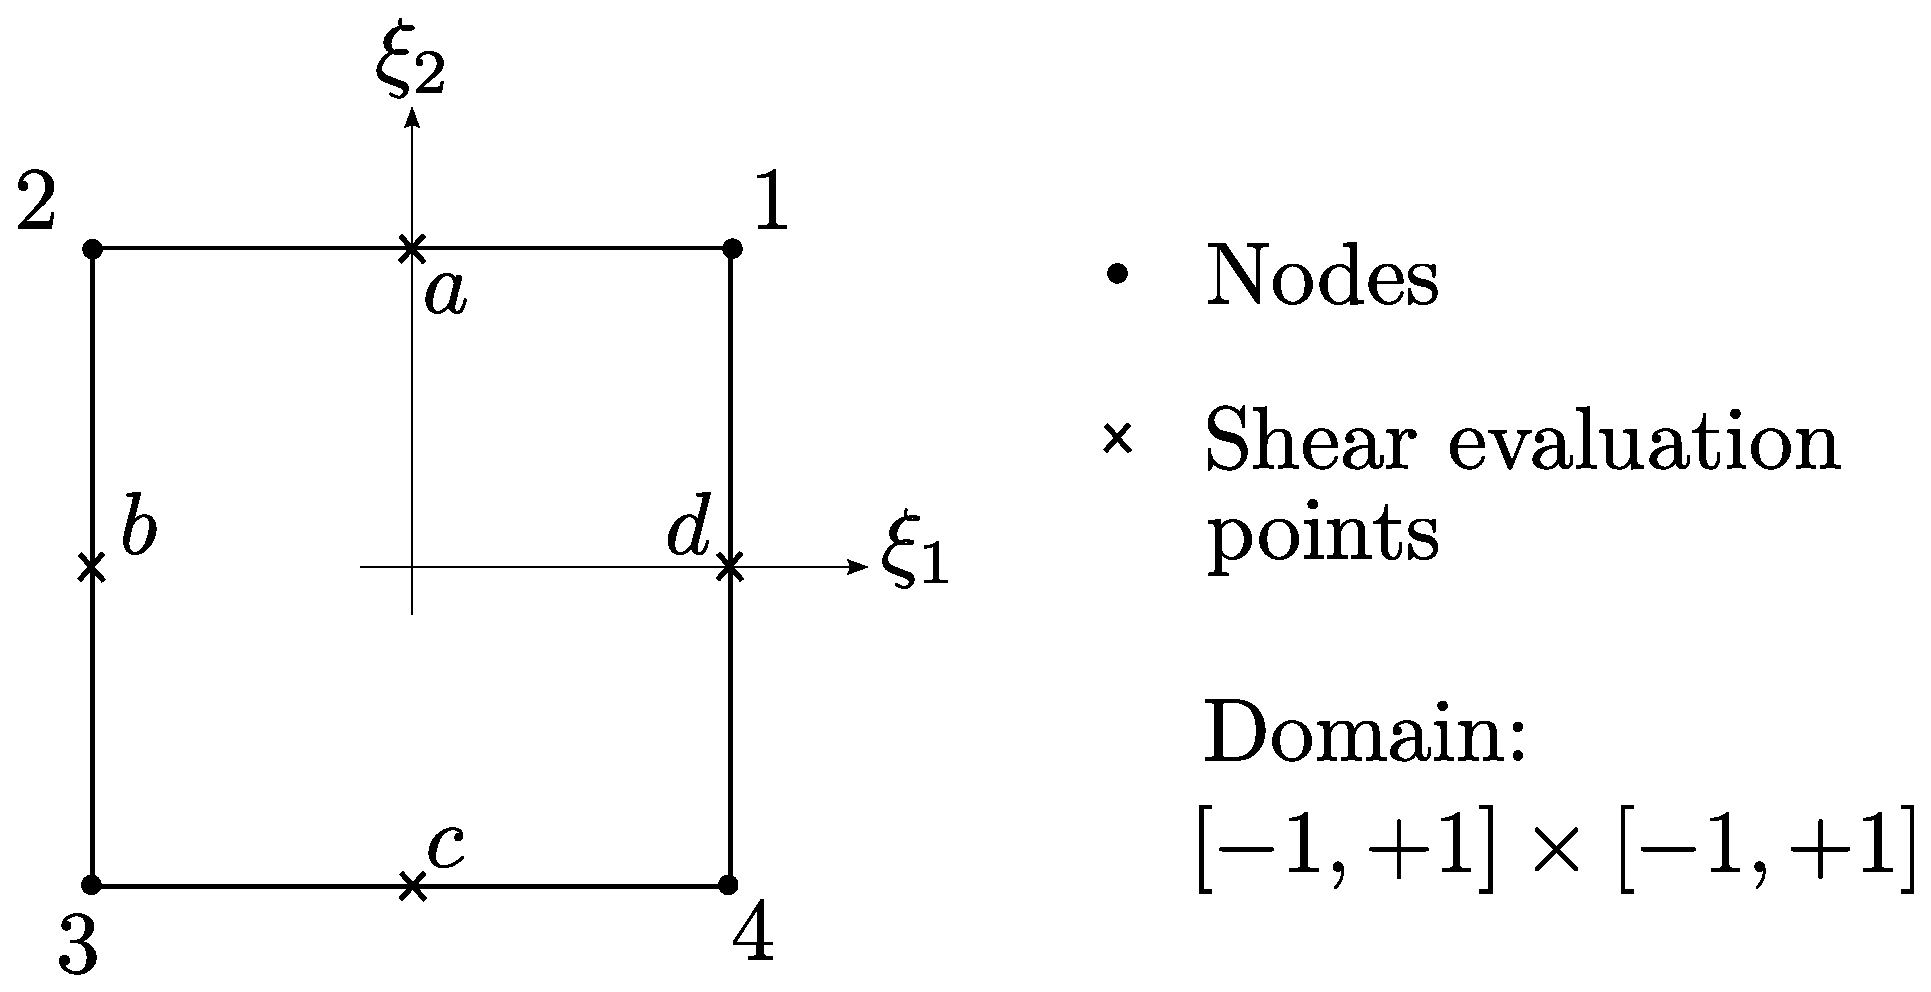
\includegraphics[width=8cm]{shellPic.eps}
\caption{Shell finite element}
\label{fig:shell}
\end{figure}
In the natural domain, the coordinate system is identified by the coordinates $\xi_1$ and $\xi_2$, both varying in the range $[-1, 1]$. \\
In the next it will be used the notation:
\begin{equation}
\T{\xi} = \plbr{\xi_{1},\xi_{2}}
\end{equation}
Four points are defined on the midsides of the element, and are used in the context of the ANS approach. In particular, they are denoted by the set of coordinates:
\begin{equation}
\vvect{c}{
\T{\xi}_a = \plbr{\xi_{1a},\xi_{2a}} \\
\T{\xi}_b = \plbr{\xi_{1b},\xi_{2b}} \\
\T{\xi}_c = \plbr{\xi_{1c},\xi_{2c}} \\
\T{\xi}_d = \plbr{\xi_{1d},\xi_{2d}}
}
\label{eq:xiSep}
\end{equation}
The following convention is adopted:
\begin{itemize}
	\item the subscript $n$ denotes a nodal variable
  \item $\T{\xi}_i$ means $\T{\xi}$ evaluated in a generic integration point
  \item $\T{\xi}_A$ means $\T{\xi}$ evaluated in one of the four shear evaluation points
  \item $\T{\xi}_0$ means $\T{\xi}$ evaluated at the origin
\end{itemize}
Accordingly to the numeration of the nodes, the bilinear shape functions defined at element level are:
\begin{subequations}
\begin{align}
L_1(\T{\xi}) & = \frac{1}{4} \plbr{ 1 + \xi_1 } \plbr{ 1 + \xi_2 } \\
L_2(\T{\xi}) & = \frac{1}{4} \plbr{ 1 - \xi_1 } \plbr{ 1 + \xi_2 } \\
L_3(\T{\xi}) & = \frac{1}{4} \plbr{ 1 - \xi_1 } \plbr{ 1 - \xi_2 } \\
L_4(\T{\xi}) & = \frac{1}{4} \plbr{ 1 + \xi_1 } \plbr{ 1 - \xi_2 }
\end{align}
\end{subequations}
The degrees of freedom associated to each element are 24 nodal positions and orientations collected in the vector ${\T{q}}$:
\begin{align}
\underset{24 \times 1}{\delta{\T{q}}}  =
\cubr{\vvect{c}{
\delta \T{y}_{n} \\
\T{\varphi}_{\delta n} \\
}}
 = &
\cubr{\vvect{c}{
\delta \T{y}_{1} \\
\T{\varphi}_{\delta 1} \\
\delta \T{y}_{2} \\
\T{\varphi}_{\delta 2} \\
\delta \T{y}_{3} \\
\T{\varphi}_{\delta 3} \\
\delta \T{y}_{4} \\
\T{\varphi}_{\delta 4} \\
}}
&
\underset{24 \times 1}{\Delta{\T{q}}}  =
\cubr{\vvect{c}{
\delta \T{y}_{n} \\
\T{\varphi}_{\Delta n} \\
}}
 = &
\cubr{\vvect{c}{
\Delta \T{y}_{1} \\
\T{\varphi}_{\Delta 1} \\
\Delta \T{y}_{2} \\
\T{\varphi}_{\Delta 2} \\
\Delta \T{y}_{3} \\
\T{\varphi}_{\Delta 3} \\
\Delta \T{y}_{4} \\
\T{\varphi}_{\Delta 4} \\
}}
\end{align}
and 7 internal degrees of freedom related to the assumed strain (EAS) and collected in the vector $\T{\beta}$.\\
The total number of degrees of freedom is so 31.
%%%%%%%%%%%%%%%%%%%%%%%%%%%%%%
%%%%%%%%%%LINEARIZATION%%%%%%%
%%%%%%%%%%%%%%%%%%%%%%%%%%%%%%
\section{Linearization}
The virtual variation of the compatible strains $\T{\epsilon}$ is obtained as:
\begin{equation}
\delta \T{\epsilon} =
\cubr{\vvect{c}{
\delta \tilde{\T{\epsilon} }_1 \\
\delta \tilde{\T{\epsilon} }_2 \\
\delta \tilde{\T{k} }_1 \\
\delta \tilde{\T{k} }_2 \\
}}
\end{equation}
In particular, the virtual variations of the linear deformation $\tilde{\T{\epsilon} }_k $ is:
\begin{equation}
\delta \tilde{\T{\epsilon} }_k  = \delta \plbr{ \T{T}^T \T{y}_{,k} } =
\sum_{i=1}^n \T{T}^T \T{y}_{,k} \times \T{\Phi}_{n} L_n \varphi_{\delta n} + \sum_{i=1}^n \T{T}^T L_{n,k} \delta \T{y}_{n}
\label{eq:delta_epsilon}
\end{equation}
where:
\begin{equation}
\T{\Phi}_{n} = \overline{\T{T}}  \tilde{ \T{\Gamma} } \tilde{ \T{\Gamma} }_n^{-1} \overline{\T{T}}^T
\end{equation}
The  virtual variations of the curvatures $\tilde{\T{k} }_k$ is:
\begin{equation}
\delta \tilde{\T{k} }_k = \delta \plbr{ \T{T}^T \T{k}_k } =
\sum_{i=1}^n \T{T}^T \T{k}_k \times \T{\Phi}_n L_n \varphi_{\delta n} + \sum_{i=1}^n \T{T}^T \T{K}_{kn} \varphi_{\delta n}
\label{eq:delta_k}
\end{equation}
where:
\begin{equation}
\T{K}_{kn} = \overline{\T{T}} \mathcal{L} \plbr{ \tilde{\T{\varphi}}, \tilde{\T{\varphi}}_{,k} } \tilde{ \T{\Gamma} }_{n}^{-1} \overline{T}^T L_n + \T{\Phi}_{n} L_{n,k}
\end{equation}
the term $L_{n,k}$ is the derivative of the $n$-th shape function with respect to the $k$-th arc-length coordinate.\\
%%%%%%%delta delta%%%%%%%
The last term of Eq.~\ref{eq:DeltadeltaW} requires the evaluation of the terms:
\begin{equation}
\begin{split}
\T{n}_k \cdot \Delta \delta \tilde{\T{\epsilon}}_k =
\T{n}_k \cdot \Delta \delta \plbr{ \T{T}^T \T{y}_{,k} } & =
\sum_{m,n=1}^{4} \varphi_{\delta n} \T{\Phi}_{n}^T L_n \T{y}_{,k} \times \plbr{ \T{T} \T{n}_k } \times \T{\Phi}_m L_m  \varphi_{\Delta n} + \\
& + \sum_{m,n=1}^{4} \varphi_{\delta n} \T{\Phi}_{n}^T L_n \plbr{\T{T} \T{n}_k} \times L_{m,k} \Delta \T{y}_{n} + \\
& - \sum_{m,n=1}^{4} \delta \T{y}_n L_{n,k} \plbr{\T{T} \T{n}_k} \times \T{\Phi}_m L_m \varphi_{\Delta m}
\end{split}
\label{eq:Deltadelta_epsilon}
\end{equation}
\begin{equation}
\begin{split}
\T{m}_k \cdot \Delta \delta \tilde{\T{k}}_k =
\T{m}_k \cdot \Delta \delta \plbr{\T{T}^T \T{k}_k} & =
\sum_{m,n=1}^{4} \varphi_{\delta n} L_n \T{\Phi}_n^T \T{k}_k \times \plbr{\T{T} \T{m}_k} \times \T{\Phi_{m}} L_m \varphi_{\Delta m} + \\
&+\sum_{m,n=1}^{4} \varphi_{\delta n} L_n \T{\Phi}_n^T \plbr{\T{T} \T{m}_k} \times \T{\Phi}_m L_{m,k} \varphi_{\Delta m}
\end{split}
\label{eq:Deltadelta_k}
\end{equation}
%%%%%%%%%%%%%%%%%%%%%%%%%%%%%%
%%%%%%%%%IMPLEMENTATION%%%%%%%
%%%%%%%%%%%%%%%%%%%%%%%%%%%%%%
\section{Implementation}
Having shown the variational principle and the linearization of strains and curvatures, it is then possible to develop the procedure to derive the jacobian matrix and the residual.
%%%%%%%%%%%%%%%%%%%%%%%%%%%%%%
%%%%%%%%%%%ORIENTATION%%%%%%%%
%%%%%%%%%%%%%%%%%%%%%%%%%%%%%%
\subsection{Orientation interpolation}
In the initial configuration it is built the matrix:
\begin{equation}
\T{ iTa }_n = \T{ R }_n^T \sqbr{ \T{ t }_{ 1n } \T{ t }_{ 2n } \T{ t }_{ 3n } }
\end{equation}
with $\T{ R }_n$ node orientation, and $\T{t}_{in}$ vectors tangent to the element surface.\\
So:
\begin{equation}
\T{T}_{n} = \T{ R }_n \T{ iTa }_n
\end{equation}
It is then calculated:
\begin{equation}
\T{ T }_{ avg } = \fracd{ 1 }{ 4 } \sum_{ n = 1 }^{ 4 } \T{ T }_n
\end{equation}
which is in general a not orthogonal matrix.\\
An orthogonal matrix can be obtained by applying:
\begin{equation}
\overline{ \T{ T } } = \Rot{ \VecRot{ \T{ T }_{avg} }  }
\end{equation}
which is then used to calculate the nodal rotation:
\begin{equation}
\tilde{ \T{ R } }_{ n } = \overline{ \T{ T } } ^T \T{ T }_n
\end{equation}
and:
\begin{equation}
\tilde{ \varphi }_n = \VecRot{ \tilde{ \T{ R } }_n }
\end{equation}
The nodal values of $\tilde{ \varphi }_n$ are interpolated by means of the shape functions:
\begin{equation}
\tilde{ \T{ \varphi } } \valxii = \sum_{ i = 1 }^{ 4 } L_n \valxii \tilde{ \T{ \varphi } }_n
\end{equation}
from which is obtained the rotation matrix at the integration point:
\begin{equation}
\tilde{ \T{ R } } \valxii = \Rot{ \tilde{ \varphi } \valxii }
\end{equation}
and finally the orientation at the integration point:
\begin{equation}
\T{ T } \valxii = \overline{ \T{ T } } \tilde{ \T{ R } } \valxii
\end{equation}
The virtual variation of $\T{\varphi}$ at the integration point is related to the nodal valeus by:
\begin{equation}
\T{ \varphi }_{\delta} \valxii =
\sum_{ n = 1 }^{ 4 } \T{ \Phi }_n \valxii L_n \valxii \varphi_{\delta n}
\end{equation}
with:
\begin{equation}
\T{ \Phi }_n \valxii =
\overline{ \T{ T } } \tilde{ \Gamma } \plbr{ \tilde{ \varphi \valxii } }  \tilde{ \Gamma } ^ {-1} \plbr{ \tilde{ \varphi }_n } \overline{ \T{ T } } ^ T
\end{equation}
Similarly the virtual variation of $\T{\varphi}$ can be obtained at the shear evaluation points as:
\begin{equation}
\T{ \varphi }_{\delta} \valxiA =
\sum_{ n = 1 }^{ 4 } \T{ \Phi }_n \valxiA L_n \valxiA \varphi_{\delta n}
\end{equation}
%%%%%%%%%%%%%%%%%%%%%%%%%%%%%%
%%%%%%%%%%%POSITION%%%%%%%%%%%
%%%%%%%%%%%%%%%%%%%%%%%%%%%%%%
\subsection{Position interpolation}
The nodal positions are so interpolated as:
\begin{equation}
\T{ y }   = \sum_{ n = 1 }^4  L_n   \T{ y }_n
\end{equation}
The derivatives with respect to the generic coordinate $\xi_k$ at the integration points is:
\begin{equation}
\fracdp{ \T{ x } \valxii }{ \xi_k }  = \sum_{ n = 1 }^4 \fracdp{ L_n \valxii }{ \xi_k } \T{ x }_n
\end{equation}
It is then possible to build the matrix:
\begin{equation}
\underset{ 2 \times 2 }{ \T{ S }_{ \alpha \beta } \valxii } =
\sqbr{ \matr{ c  c  }{
\underset{ 1 \times 3 }{ \T{ t }_{1}^{0} \valxii } \underset{ 3 \times 1 }{ \fracdp{ \T{x} \valxii }{ \xi_1 } } & \T{ t }_{1}^{0} \valxii \fracdp{ \T{x} \valxii }{ \xi_2 } \\
\T{ t }_{2}^{0} \valxii \fracdp{ \T{x} \valxii }{ \xi_1 } & \T{ t }_{2}^{0} \valxii \fracdp{ \T{x} \valxii }{ \xi_2 }
}}
\end{equation}
observing that $\T{T}_0 \valxii = \sqbr{ \T{t}_{1}^{0} \valxii  \T{t}_{2}^{0} \valxii \T{t}_{3}^{0} \valxii }$.\\
With the same procedure are derived $\T{ S }_{ \alpha \beta } \valxio$ and  $\T{ S }_{ \alpha \beta } \valxiA$.\\
\begin{equation}
\underset{ 4 \times 2 } { \T{ L }_{ \alpha B } \valxii } =
\sqbr{ \matr{ c c }{
\fracdp{ L_1 \valxii }{ \xi_1 } & \fracdp{ L_1 \valxii }{ \xi_2 } \\
\fracdp{ L_2 \valxii }{ \xi_1 } & \fracdp{ L_2 \valxii }{ \xi_2 } \\
\fracdp{ L_3 \valxii }{ \xi_1 } & \fracdp{ L_3 \valxii }{ \xi_2 } \\
\fracdp{ L_4 \valxii }{ \xi_1 } & \fracdp{ L_4 \valxii }{ \xi_2 } \\
}}
\end{equation}
\begin{equation}
\underset{ 4 \times 2 } { \T{ L }_{ \alpha \beta } \valxii }=
\T{ L }_{ \alpha B } \valxii \T{S}_{\alpha \beta} ^{-1} \valxii
\end{equation}
which is the matrix giving the variation of the shape functions $L_n$ with respect the the arc-length coordinates:
\begin{equation}
\T{L}_{\alpha \beta} =
\sqbr{ \matr{ c c }{
L_{1,1} & L_{1,2} \\
L_{2,1} & L_{2,2} \\
L_{3,1} & L_{3,2} \\
L_{4,1} & L_{4,2}
}}
\end{equation}
In order to perform the integration in the isoparametric domain the area element need to be calculated. In particular, the determinant of the jacobian of the transformation between the physical and the natural domain has to be calculated. It is:
\begin{align}
\alpha \valxii & = \det \T{ S }_{\alpha \beta} \valxii &
\alpha \valxiA & = \det \T{ S }_{\alpha \beta} \valxiA
\end{align}
%%%%%%%%%%%%%%%%%%%%%%%%%%%%%%
%%%%%%%%%%%%EAS%%%%%%%%%%%%%%%
%%%%%%%%%%%%%%%%%%%%%%%%%%%%%%
\subsection{Enhancing strains interpolation}
The virtual variation and increments of the enhancing strains $\T{\hat{\epsilon}}$ are interpolated as:
\begin{align}
\underset{12 \times 1}{\delta \hat{\T{\epsilon}}} \valxii & = \underset{12 \times 7}{\T{P}} \valxii \underset{7 \times 1}{ \delta \T{\beta}} &  \Delta \hat{\T{\epsilon}}\valxii & = \T{P}\valxii \Delta \T{\beta}
\end{align}
where $\T{\beta}$ is the vector collecting the the strains parameters, while the expression of the matrix $\T{P}$ is derived in the next. \\
The EAS approach here adopted considers the enhancing of the membrane strains only, i.e. $\epsilon_{11}$, $\epsilon_{12}$, $\epsilon_{21}$ and $\epsilon_{22}$. Shear strains and bending strains are not enhanced.\\
The interpolation is performed in the natural domain adopting the shape functions:
\begin{equation}
\underset{ 4 \times 7 } { \T{ H } \valxii } =
\sqbr{ \matr{ c c c c c c c }{
\xi_{1i} & \xi_{1i} \xi_{2i} &  0    &      0      &   0   &      0      &   0     \\
  0   &      0      & \xi_{2i} & \xi_{1i} \xi_{2i} &   0   &      0      &   0     \\
  0   &      0      &  0    &      0      & \xi_{1i} & \xi_{1i} \xi_{2i} &   0      \\
  0   &      0      &  0    &      0      &   0   & \xi_{1i} \xi_{2i} & \xi_{2i}
}}
\end{equation}
The interpolation is reported in the pyshical domain with a push-forward operation with the transformation matrix $\T{M}_0$, defined as:
\begin{equation}
\underset{ 4 \times 4 } { \T{M}_0 } =
\sqbr{ \matr{ c c c c}{
s_{ 1, 1 } s_{ 1, 1 } & s_{ 1, 2 } s_{ 1, 2 } & s_{ 1, 2 } s_{ 1, 1 } &  s_{ 1, 1 } s_{ 1, 2 } \\
s_{ 2, 1 } s_{ 2, 1 } & s_{ 2, 2 } s_{ 2, 2 } & s_{ 2, 2 } s_{ 2, 1 } &  s_{ 2, 1 } s_{ 2, 2 } \\
s_{ 1, 1 } s_{ 2, 1 } & s_{ 1, 2 } s_{ 2, 2 } & s_{ 1, 1 } s_{ 2, 2 } &  s_{ 1, 2 } s_{ 2, 1 } \\
s_{ 1, 1 } s_{ 2, 1 } & s_{ 1, 2 } s_{ 2, 2 } & s_{ 1, 2 } s_{ 2, 1 } &  s_{ 1, 1 } s_{ 2, 2 }
}}
\end{equation}
where the generic term $s_{ i, k }$ is the element $\plbr{i,k}$ of the matrix $\T{ S }_{ \alpha \beta } \valxio$.\\
\begin{equation}
\underset{ 12 \times 7 }{ \T{ P } \valxii } =
\fracd{ \alpha \valxio }{ \alpha \valxii } \underset{ 12 \times 4  }{ \T{\mathcal{P}} } \underset{ 4 \times 4 }{ \T{ M }_{0}^{-T} } \underset{ 4 \times 7 }{ \T{H} \valxii }
\end{equation}
where $\T{\mathcal{P}}$ is a permutation matrix defined as:

\begin{equation}
\underset{ 12 \times 7 }{ \T{\mathcal{P}} } =
\sqbr{ \matr{ c c c c  }{
1 & 0 & 0 & 0 \\
0 & 0 & 1 & 0 \\
0 & 0 & 0 & 0 \\
0 & 0 & 0 & 1 \\
0 & 0 & 0 & 0 \\
0 & 0 & 0 & 0 \\
0 & 0 & 0 & 0 \\
0 & 0 & 0 & 0 \\
0 & 0 & 0 & 0 \\
0 & 0 & 0 & 0 \\
0 & 0 & 0 & 0 \\
0 & 0 & 0 & 0
}}
\end{equation}
which has the places the enhanced strains in the corresponding positions of the global vector of membrane and bending strains $\T{\epsilon}$.
%%%%%%%%%%%%%%%%%%%%%%%%%%%%%%
%%%%%COMAPTIBLE STRAINS%%%%%%
%%%%%%%%%%%%%%%%%%%%%%%%%%%%%%
\subsection{Compatible strains interpolation}
The virtual variations of the linear deformation $\tilde{\T{\epsilon} }_k $ at the $i$-th integration point is obtained from Eq.~\ref{eq:delta_epsilon}:
\begin{equation}
\begin{split}
\delta \tilde{\T{\epsilon} }_k \valxii & = \delta \plbr{ \T{T}\valxii^T \T{y}_{,k} \valxii } = \\
& \sum_{i=1}^n \T{T}\valxii^T \T{y}_{,k}\valxii \times \T{\Phi}_{n} \valxii L_n \valxii \varphi_{n \delta} + \sum_{i=1}^n \T{T}\valxii^T \T{L}_{\alpha \beta} \valxii \plbr{ n, k } \valxii \delta \T{y}_{n}
\end{split}
\label{eq:delta_epsilon_i}
\end{equation}
where $\T{L}_{\alpha \beta} \valxii \plbr{ n, k }$ denotes the element $\plbr{n, k}$ of the matrix $\T{L}_{\alpha \beta} \valxii$.\\
The  virtual variation of the curvatures $\tilde{\T{k} }_k$ at the $i$-th integration point is derived from Eq.~\ref{eq:delta_k}:
\begin{equation}
\begin{split}
\delta \tilde{\T{k} }_k \valxii & = \delta \plbr{ \T{T}\valxii^T \T{k}_k \valxii} =  \\
& \sum_{i=1}^n \T{T}\valxii^T \T{k}_k\valxii \times \T{\Phi}_n\valxii L_n\valxii \varphi_{n \delta} + \sum_{i=1}^n \T{T}\valxii^T \T{K}_{kn}\valxii \varphi_{n \delta}
\end{split}
\label{eq:delta_k_i}
\end{equation}
where:
\begin{equation}
\T{\Phi}_{n} \valxii = \overline{\T{T}}  \tilde{ \T{\Gamma} } \plbr{ \tilde{\varphi} \valxii } \tilde{ \T{\Gamma} }_n^{-1} \overline{\T{T}}^T
\end{equation}
and:
\begin{equation}
\T{K}_{kn} \valxii =
\overline{\T{T}} \mathcal{L} \plbr{ \tilde{\T{\varphi}}\valxii, \tilde{\T{\varphi}}_{,k}\valxii } \tilde{ \T{\Gamma} }_{n}^{-1} \overline{T}^T L_n\valxii + \T{\Phi}_{n}\valxii \T{L}_{\alpha \beta} \valxii \plbr{ n, k } \valxii
\end{equation}
The derivative of the the vector $\tilde{\T{\varphi}}$ with respect to the $k$-th arc-length coordinate can be expressed as function of the nodal values as:
\begin{equation}
\tilde{ \T{ \varphi } }_{,k} \valxii  =
\sum_{n=1}^4 \T{L}_{\alpha \beta} \valxii \plbr{ n, k } \T{\varphi}_{n}
\end{equation}
The curvatures are given by:
\begin{equation}
\T{k}_{k} \valxii  =
\overline{\T{T}} \tilde{\Gamma} \plbr{ \tilde{\varphi} \valxii } \tilde{ \varphi }_{,k} \valxii
\end{equation}
and the derivative of the position vector is:
\begin{equation}
\T{y}_{,k} \valxii  =
\sum_{i=1}^{4} \T{L}_{\alpha \beta} \valxii \plbr{n,k} \T{y}_n
\end{equation}
The compatible strains can so be expressed as function of the nodal variables $\T{q}$ by considering Eqs.~\ref{eq:delta_epsilon_i} and \ref{eq:delta_k_i}:
\begin{equation}
\delta \T{\epsilon} = \overline{\T{B}} \delta{\T{q}}
\end{equation}
with:
\begin{equation}
\underset{ 12 \times 24 }{\overline{\T{B}} \valxii} =
\sqbr{ \matr{ c c c c  }{
\overline{\T{B}}_1 \valxii & \overline{\T{B}}_2 \valxii & \overline{\T{B}}_3 \valxii & \overline{\T{B}}_4 \valxii
}}
\label{eq:B_overline}
\end{equation}
and:
\begin{equation}
\underset{ 12 \times 6 }{\overline{\T{B}}_n \valxii} =
\sqbr{ \matr{ c c  }{
\T{T} \valxii^T \T{L}_{\alpha \beta} \valxii \plbr{n,1} & \T{T}\valxii^T \T{y}_{,1} \valxii \times \T{\Phi}_{n} \valxii L_{n} \valxii \\
\T{T} \valxii^T \T{L}_{\alpha \beta} \valxii \plbr{n,2} & \T{T}\valxii^T \T{y}_{,2} \valxii \times \T{\Phi}_{n} \valxii L_{n} \valxii \\
0 & \T{T}\valxii^T \T{k}_{1} \valxii \times \T{\Phi}_{n} \valxii L_{n} \valxii + \T{T} \valxii^T \T{K}_{1n} \valxii \\
0 & \T{T}\valxii^T \T{k}_{2} \valxii \times \T{\Phi}_{n} \valxii L_{n} \valxii + \T{T} \valxii^T \T{K}_{2n} \valxii
}}
\end{equation}
%%%%%%%%%%%%%%%%%%%%%%%%%%%%%%
%%%%%%%%%%ANS%%%%%%%%%%%%%%%%%
%%%%%%%%%%%%%%%%%%%%%%%%%%%%%%
\subsection{ANS}
The ANS technique is applied to prevent shear locking. Here the ANS is applied to shear strains only, i.e. $\epsilon_{1}$ and  $\epsilon_{2}$ The approach consists in interpolating the shear strains in the midsides of the element in the natural domain. Such interpolated strains are then used to derive the shear strains at the integration points.\\
The use of the ANS technique leads a re-definition of:
\begin{itemize}
	\item the two rows of the $\overline{\T{B}}$ matrix relative to shear strains
	\item the shear strains
\end{itemize}
The compatible strains are:
\begin{align}
\tilde{\T{\epsilon}}_1 & =
\cubr{\vvect{c}{
\epsilon_{11} \\
\epsilon_{12} \\
\epsilon_{1}
}}
&
\tilde{\T{\epsilon}}_2 & =
\cubr{\vvect{c}{
\epsilon_{21} \\
\epsilon_{22} \\
\epsilon_{2}
}}
\end{align}
At first, the compatible strains are evaluated at the shear evaluation points of Figure~\ref{fig:shell}. This is done referring to Eq.~\ref{eq:epsilon}
\begin{equation}
\tilde{\T{\epsilon}}_k \valxiA  =
\T{T} \valxiA ^T \T{y}_{,k} \valxiA - \T{e}_k
\end{equation}
The matrix $\overline{\T{B}}$ of Eq.~\ref{eq:B_overline} is built also in the shear evaluation points for the membrane strains only, and is indicated as $\overline{\overline{\T{B}}}$
\begin{equation}
\underset{ 6 \times 24 }{\overline{\overline{\T{B}}} \valxiA} =
\sqbr{ \matr{ c c c c  }{
\overline{\overline{\T{B}}}_1 \valxiA & \overline{\overline{\T{B}}}_2 \valxiA & \overline{\overline{\T{B}}}_3 \valxiA & \overline{\overline{\T{B}}}_4 \valxiA
}}
\end{equation}
with:
\begin{equation}
\underset{ 6 \times 6 }{\overline{\overline{\T{B}}}_n \valxiA} =
\sqbr{ \matr{ c c  }{
\T{T} \valxiA ^ T \T{L}_{\alpha \beta} \valxiA \plbr{n,1} & \T{T} \valxiA^T \T{y}_{,1} \valxiA \times \T{\Phi}_{n} \valxiA L_{n}  \valxiA \\
\T{T} \valxiA ^ T \T{L}_{\alpha \beta} \valxiA \plbr{n,2} & \T{T} \valxiA^T \T{y}_{,2} \valxiA \times \T{\Phi}_{n} \valxiA L_{n}  \valxiA
}}
\end{equation}
The rows relative to the shear strains $\epsilon_1$ and $\epsilon_2$ are collected in:
\begin{align}
\underset{ 4 \times 24 }{\overline{\overline{\T{B3}}} \valxiA} & =
\sqbr{ \matr{ c c  }{
\overline{\overline{\T{B}}} \plbr{ \T{\xi}_a } \plbr{3,:} \\
\overline{\overline{\T{B}}} \plbr{ \T{\xi}_b } \plbr{3,:} \\
\overline{\overline{\T{B}}} \plbr{ \T{\xi}_c } \plbr{3,:} \\
\overline{\overline{\T{B}}} \plbr{ \T{\xi}_d } \plbr{3,:}
}}
&
\underset{ 4 \times 24 }{\overline{\overline{\T{B6}}} \valxiA} & =
\sqbr{ \matr{ c c  }{
\overline{\overline{\T{B}}} \plbr{ \T{\xi}_a } \plbr{6,:} \\
\overline{\overline{\T{B}}} \plbr{ \T{\xi}_b } \plbr{6,:} \\
\overline{\overline{\T{B}}} \plbr{ \T{\xi}_c } \plbr{6,:} \\
\overline{\overline{\T{B}}} \plbr{ \T{\xi}_d } \plbr{6,:}
}}
\end{align}
where $\overline{\overline{\T{B}}} \plbr{ \T{\xi}_a } \plbr{k,:}$ is used to denote all the element of the $k$-th row of $\overline{\overline{\T{B}}} \plbr{ \T{\xi}_a }$.\\
The matrices $\overline{\overline{\T{B3}}}$ and $\overline{\overline{\T{B6}}}$ are interpolated to obtain the values at the integration points.
\begin{align}
\overline{\T{B3}} \valxii & = \fracd{1}{2}
\sqbr{ \matr{ c c c c  }{
1 + \xi_{2i} & 0 & 1 - \xi_{2i} & 0
}}
\overline{\overline{\T{B3}}} \valxiA
\\
\overline{\T{B6}} \valxii & = \fracd{1}{2}
\sqbr{ \matr{ c c c c  }{
1 + \xi_{1i} & 0 & 1 - \xi_{1i} & 0
}}
\overline{\overline{\T{B6}}} \valxiA
\end{align}
The obtained matrices $\overline{\T{B3}}$ and $\overline{\T{B6}}$ replace the corresponding rows of the matrix $\overline{\T{B}}$ of Eq.~\ref{eq:B_overline}.\\
The second step in the application of the ANS technique is the interpolation of the shear strains:
\begin{subequations}
\begin{align}
\epsilon_1 \valxii & =
\fracd{1}{2} \plbr{ 1 + \xi_{2i} } \epsilon_1 \plbr{ \T{\xi}_a } + \fracd{1}{2} \plbr{1-\xi_{2i}} \epsilon_1 \plbr{ \T{\xi}_c } \\
\epsilon_2 \valxii & =
\fracd{1}{2} \plbr{ 1 - \xi_{1i} } \epsilon_2 \plbr{ \T{\xi}_b } + \fracd{1}{2} \plbr{1+\xi_{1i}} \epsilon_2 \plbr{ \T{\xi}_d }
\end{align}
\end{subequations}
The so interpolated strains $\epsilon_1$ and $\epsilon_2$ are then inserted into the proper position in the vector $\T{\epsilon}$ respectively.\\
%%%%%%%%%%%%%%%%%%%%%%%%%%%%%%
%%%%%%%%%%%FORCES%%%%%%%%%%%%%
%%%%%%%%%%%%%%%%%%%%%%%%%%%%%%
\subsection{Forces}
Strains and curvatures can be calculated as:
\begin{equation}
\tilde{\T{\epsilon}}_k \valxii  =
\T{T} \valxii ^T \T{y}_{,k} \valxii - \T{e}_k
\end{equation}
\begin{equation}
\tilde{\T{k}}_k  =
\T{T} \valxii ^ T \T{k}_k \valxii - \T{T}_0 ^ T \valxii \T{k}^{0}_{k} \valxii
\end{equation}
where $\T{T}_0$ and $\T{k}^{0}_{k}$ are calculated at the first step.\\
The total strain is the sum of the compatible and the enhancing strains:
\begin{equation}
\T{\epsilon}_t \valxii =
\T{\epsilon} \valxii +
\hat{ \T{\epsilon} } \valxii
\end{equation}
The resulting forces are easily computed by means of the constitutive law:
\begin{equation}
\T{\sigma} \valxii =
\T{C}\valxii \T{\epsilon}_t \valxii
\end{equation}
which is:
\begin{equation}
\T{\sigma} \valxii =
\cubr{\vvect{c}{
\T{n}_1 \valxii \\
\T{n}_2 \valxii \\
\T{m}_1 \valxii \\
\T{m}_2 \valxii
}}
\end{equation}
%%%%%%%%%%%%%%%%%%%%%%%%%%%%%%
%%%%%%%%%%%JACOBIAN%%%%%%%%%%%
%%%%%%%%%%%%%%%%%%%%%%%%%%%%%%
\subsection{Jacobian matrix}
The second variation of the variational principle of Eq.~\ref{eq:DeltadeltaW} gives the jacobian matrix. In particular, the finite element discretization is here presented for the five different terms of Eq.~\ref{eq:DeltadeltaW}.\\
The first term is:
\begin{equation}
\begin{split}
\int_A \delta {\T{\epsilon}} ^T  \T{C}  \Delta {\T{\epsilon}}  dA & = \\
& = \delta{\T{q}}^T  \sum_{i=1}^{4} \overline{\T{B}}\valxii^T  \T{C}\valxii  \overline{\T{B}}\valxii  \alpha \valxii   w_i \Delta \T{q} \\
& = \delta{\T{q}}^T  \T{K}_m  \Delta \T{q}
\end{split}
\end{equation}
The second term is:
\begin{equation}
\begin{split}
\int_A  \delta \hat{{\T{\epsilon}}} ^T  \T{C}  \Delta {\T{\epsilon}} dA & = \\
& = \delta{\T{\beta}}^T  \sum_{i=1}^{4} \T{P}\valxii^T  \T{C}\valxii  \overline{\T{B}}\valxii  \alpha \valxii  w_i \Delta \T{q} \\
& = \delta{\T{\beta}}^T  \T{K}_{\beta q}  \Delta \T{q}
\end{split}
\end{equation}
The third term is:
\begin{equation}
\begin{split}
\int_A \delta {\T{\epsilon}} ^T  \T{C}  \Delta \hat{{\T{\epsilon}}} dA & = \\
& = \delta{\T{q}}^T  \T{K}_{\beta q}^T  \Delta \T{\beta}
\end{split}
\end{equation}
The fourth term is:
\begin{equation}
\begin{split}
\int_A \delta \hat{{\T{\epsilon}}} ^T  \T{C}  \Delta \hat{{\T{\epsilon}}} dA & = \\
& = \delta{\T{\beta}}^T  \sum_{i=1}^{4} \T{P}\valxii^T  \T{C}\valxii  \T{P}\valxii  \alpha \valxii  w_i \Delta \T{\beta} \\
& = \delta{\T{\beta}}^T  \T{K}_{\beta \beta}  \Delta \T{\beta}
\end{split}
\end{equation}
The fifth term is:
\begin{equation}
\begin{split}
\int_A \Delta \delta { \T{\epsilon} }^T \T{\sigma} dA & = \\
& = \delta{\T{q}}^T  \sum_{i=1}^{4} \overline{\T{D}}\valxii^T  \T{G}\valxii  \overline{\T{D}}\valxii  \alpha \valxii  w_i \Delta \T{q} \\
& = \delta{\T{q}}^T  \T{K}_g  \Delta \T{q}
\end{split}
\end{equation}
where this last expression is obtained starting from Eqs.~\ref{eq:Deltadelta_epsilon} and \ref{eq:Deltadelta_k}, and where:
\begin{equation}
\underset{ 15 \times 24 }{\overline{\T{D}} \valxii} =
\sqbr{ \matr{ c c c c  }{
\overline{\T{D}}_1 \valxii & \overline{\T{D}}_2 \valxii & \overline{\T{D}}_3 \valxii & \overline{\T{D}}_4 \valxii
}}
\end{equation}
with:
\begin{equation}
\underset{ 15 \times 6 }{\overline{\T{D}}_n \valxii} =
\sqbr{ \matr{ c c  }{
\T{L}_{\alpha \beta} \valxii \plbr{n,1} \T{I} & \T{0} \\
\T{L}_{\alpha \beta} \valxii \plbr{n,2} \T{I} & \T{0} \\
\T{0} & \T{K}_{1n} \valxii\\
\T{0} & \T{K}_{2n} \valxii \\
\T{0} & \T{\Phi}_{n} \valxii L_{n} \valxii \\
}}
\end{equation}
\begin{equation}
\begin{split}
\T{Hh} \valxii & =
\T{T} \valxii \T{n}_1 \valxii \otimes \T{y}_{,1} \valxii - \T{T} \valxii \T{n}_1 \cdot \T{y}_{,1} \valxii \T{I} + \\
& + \T{T} \valxii \T{n}_2 \valxii \otimes \T{y}_{,2} \valxii - \T{T} \valxii \T{n}_2 \cdot \T{y}_{,2} \valxii \T{I} + \\
& + \T{T} \valxii \T{m}_1 \valxii \otimes \T{k}_{1} \valxii - \T{T} \valxii \T{m}_1 \cdot \T{k}_{1} \valxii \T{I} + \\
& + \T{T} \valxii \T{m}_2 \valxii \otimes \T{k}_{2} \valxii - \T{T} \valxii \T{m}_2 \cdot \T{k}_{2} \valxii \T{I}
\end{split}
\end{equation}
\begin{equation}
\underset{ 15 \times 15 }{ \T{G} \valxii } =
\sqbr{ \matr{ c c c c c}{
\T{0} & \T{0} & \T{0} & \T{0} & -\T{T} \valxii \T{n}_1 \valxii \\
\T{0} & \T{0} & \T{0} & \T{0} & -\T{T} \valxii \T{n}_2 \valxii \\
\T{0} & \T{0} & \T{0} & \T{0} & -\T{T} \valxii \T{n}_1 \valxii \\
\T{0} & \T{0} & \T{0} & \T{0} &  \T{0} \\
\T{0} & \T{0} & \T{0} & \T{0} &  \T{0} \\
\T{T} \valxii \T{n}_1 \valxii & \T{T} \valxii \T{n}_2 \valxii & \T{T} \valxii \T{m}_1 \valxii &  \T{T} \valxii \T{m}_2 \valxii & \T{Hh} \valxii
}}
\end{equation}
%%%%%%%%%%%%%%%%%%%%%%%%%%%%%%
%%%%%%%%%RESIDUAL%%%%%%%%%%%%%
%%%%%%%%%%%%%%%%%%%%%%%%%%%%%%
\subsection{Residual}
The residual comes from the finite element approximation of Eq.~\ref{eq:deltaW}. \\
The first term is:
\begin{equation}
\begin{split}
\int_A \delta{\T{\epsilon}}^T \T{\sigma} dA & = \\
& = \delta \T{q}^T \sum_{i=1}^{4} \overline{\T{B}}\valxii^T  \T{\sigma}\valxii  \alpha \valxii  w_i \\
& = \delta \T{q}^T \T{r}_{d}
\end{split}
\end{equation}
The second term is:
\begin{equation}
\begin{split}
\int_A \delta \hat{\T{\epsilon}}^T \T{\sigma} dA & = \\
& = \delta \T{\beta}^T \sum_{i=1}^{4} \T{P}\valxii^T  \T{\sigma}\valxii  \alpha \valxii  w_i \\
& = \delta \T{\beta}^T \T{r}_{\beta}
\end{split}
\end{equation}
The resulting governing equations are then:
\begin{subequations}
\begin{align}
\plbr{ \T{K}_m + \T{K}_g } \Delta \T{q} + \T{K}_{\beta q} ^ T \Delta \T{\beta} & = - \T{r}_{d} \\
\T{K}_{\beta q}  \Delta \T{q} + \T{K}_{\beta \beta}  \Delta \T{\beta} & = - \T{r}_{\beta} \\
\end{align}
\end{subequations}




\chapter{Aerodynamic Elements}
% MBDyn (C) is a multibody analysis code.
% http://www.mbdyn.org
%
% Copyright (C) 1996-2009
%
% Pierangelo Masarati  <masarati@aero.polimi.it>
%
% Dipartimento di Ingegneria Aerospaziale - Politecnico di Milano
% via La Masa, 34 - 20156 Milano, Italy
% http://www.aero.polimi.it
%
% Changing this copyright notice is forbidden.
%
% This program is free software; you can redistribute it and/or modify
% it under the terms of the GNU General Public License as published by
% the Free Software Foundation (version 2 of the License).
% 
%
% This program is distributed in the hope that it will be useful,
% but WITHOUT ANY WARRANTY; without even the implied warranty of
% MERCHANTABILITY or FITNESS FOR A PARTICULAR PURPOSE.  See the
% GNU General Public License for more details.
%
% You should have received a copy of the GNU General Public License
% along with this program; if not, write to the Free Software
% Foundation, Inc., 59 Temple Place, Suite 330, Boston, MA  02111-1307  USA
%
% Alessandro Fumagalli <fumagalli@aero.polimi.it> is the author of this document

Aerodynamic elements apply aerodynamic forces to structural nodes.

This section is not intended 
to give details about the aerodynamic models adopted but mainly 
discuss the computation of the contributions to the Jacobian 
matrix of the aerodynamic elements.

\paragraph{Files.} \
It is implemented in files\\
\begin{tabular}{l}
\texttt{mbdyn/aero/aeroelem.h} \\
\texttt{mbdyn/aero/aeroelem.cc} 
\end{tabular}

\paragraph{Aerodynamic body}
%\section{Aerodynamic Body}

The \texttt{aerodynamic body} element applies aerodynamic forces
to the structural node it is connected to,
based on the relative velocity between an aerodynamic surface attached 
to the node and the airstrem.

The aerodynamic forces and moments acting on the attached node are:
\begin{subequations}
\begin{align}
	\T{f} &= \TT{R}_{\text{loc}} \T{f}_a\\ 
	\T{c} &= \TT{R}_{\text{loc}} \T{c}_a + \T{x}_r\times\T{f} 
\end{align}
\end{subequations}
where $\TT{R}_{\text{loc}} = \TT{R}_n\TT{R}_a\TT{R}_t$ is the orientation 
matrix from the local frame of the aerodynamics to the global, 
while $\T{f}_a$ and $\T{c}_a$ are the aerodynamic force and moment 
respectively in the reference frame of the aerodynamics. $\TT{R}_n$
is the orientation matrix of the node, $\TT{R}_a$ is the
relative orientation matrix of the aerodynamics frame with respect 
to the node frame while $\TT{R}_t$ is a rotation matrix 
related to the twist of the aerodynamic surface.
Both $\TT{R}_a$ and $\TT{R}_t$ do not depend on the unknowns
olf the problem, and thus their perturbation is zero.
The vector $\T{x}_r = \TT{R}_n\T{b}$ is the offset of the aerodynamic
surface with respect to the node; $\T{b}$ is constant.

The aerodynamic forces and moments are computed as functions 
of a velocity vector in the reference frame of the aerodynamics:
\begin{equation}\label{eq:fa=g(va)}
	\sqbr{\matr{c}{\T{f_a}\\\T{c_a}}} = \T{g}\plbr{\T{V}_{a}}
\end{equation}
where $\T{V}_{a} = \sqbr{\T{v}_a^T\ \T{\omega}_a^T}^T$ includes both the 
linear and angular velocity in the reference frame of the aerodynamics:
\begin{equation}
	\T{V}_{a} = \sqbr{\matr{c}{
		\TT{R}^T_{\text{loc}} \plbr{\T{v}_n + \T{\omega}_n\times\T{x}_r - \T{v}_{\infty} - \T{v}_{\text{ind}}}\\
		\TT{R}^T_{\text{loc}} \T{\omega}_n
		}}
\end{equation}
The total airstream velocity in the aerodynamic frame of reference 
includes also the free stream velocity $\T{v}_{\infty}$ and
the induced velocity $\T{v}_{\text{ind}}$, were the aerodynamic element
connected to any induced velocity model.
These two contributions will not be considered in the following
since they do not depend on the unknowns of the problem\footnote{In general,
induced velocity models depend on the aerodynamic loads,
and thus may indirectly depend on the unknowns of the problem.
This dependence is neglected.
}, and thus do not contribute to the Jacobian matrix of the problem. 

The perturbation of the aerodynamic force in the global reference frame
yields:
\begin{align}
	\delta\T{f}
	& = \T{\theta}_{\delta}\times\TT{R}_{\text{loc}}\T{f}_a
	+ \TT{R}_{\text{loc}}\frac{\partial\T{f}_a}{\partial\T{V}_a}
		\delta\T{V}_a
	\nonumber \\
	&= \T{\theta}_{\delta}\times \T{f}
	+ \TT{R}_{\text{loc}}\frac{\partial\T{f}_a}{\partial\T{V}_a}
		\delta\T{V}_a
\end{align}
The $3\times6$ matrix $\partial\T{f}_a/\partial\T{V}_a$, 
named $\T{J_f}_a$ in the
following, is computed numerically using the finite difference method
described below.

The perturbation of the aerodynamic moment in the global reference frame
yields:
\begin{align}
	\delta\T{c}
	&= \T{\theta}_{\delta}\times\TT{R}_{\text{loc}}\T{c}_a
	+ \TT{R}_{\text{loc}}\frac{\partial\T{c}_a}{\partial\T{V}_a}
		\delta\T{V}_a
	+ \delta\T{x}_r\times\T{f}
	+ \T{x}_r\times\delta\T{f}
	\nonumber \\
	&= \T{\theta}_{\delta}\times\T{c}
	+ \TT{R}_{\text{loc}}\frac{\partial\T{c}_a}{\partial\T{V}_a}
		\delta\T{V}_a
	+ \T{x}_r\times
		\TT{R}_{\text{loc}}\frac{\partial\T{f}_a}{\partial\T{V}_a}
		\delta\T{V}_a
	\nonumber \\
	&= \T{\theta}_{\delta}\times\T{c}
	+ \TT{R}_{\text{loc}}\plbr{
		\frac{\partial\T{c}_a}{\partial\T{V}_a}
		+ \T{b}\times\frac{\partial\T{f}_a}{\partial\T{V}_a}
	} \delta\T{V}_a
\end{align}
The $3\times6$ matrix $\partial\T{c}_a/\partial\T{V}_a$, 
named $\T{J_c}_a$ in the
following, is computed numerically as well, using a finite difference method.

The Jacobian matrix of the aerodynamic forces and moments in the reference 
frame of the aerodynamics is computed computed numerically,
using a forward finite difference method involving a numerical perturbation
of the relative velocity in the reference frame of the aerodynamics.
In detail, each component of the $6\times6$ matrix $\T{J}_a$ is computed as:
\begin{equation}
	{J_a}_{ij} = \frac{g_i(\T{V}_a + \Delta\T{V}_a) 
		- g_i(\T{V}_a)}{\Delta {V_a}_j}
\end{equation}
The perturbation of the velocity, $\Delta\T{V}_a$ in this case, plays
a crucial role. The procedure here adopted consists in obtaining this
perturbation based on the norm of the linear velocity $\T{v}_a$ for what 
concerns the perturbation of the linear velocity components, based on
the norm of the angular velocity $\T{\omega}_a$ for what concerns 
the angular velocity components. Thus:
\begin{equation}
	\Delta {V_a}_j = \Bigl\{\matr{c}{
		\varepsilon\lvert\T{v}_a\lvert\text{ if $j = 1,2,3$}\\
		\varepsilon\lvert\T{\omega}_a\lvert\text{ if $j = 4,5,6$}
		}
\end{equation}
To summarize the procedure, it can be helpful to report the algorithm
actually implemented:
\begin{verbatim}
F0a = GetForces(V0a);
for(i = 1; i <= 6; i++)	{
    deltaVa = V0a; 
				
    if (i <= 3)	{
        delta = norm(V0a) * epsilon;
    } else		{
        delta = norm(W0a) * epsilon;
    }
    deltaVa(i) = V0a(i) + delta;
					
    Fa = GetForces(deltaVa);
	
    for(j = 1; j <= 6; j++)	{
        Ja(j,i) = (Fa(j) - Fa0(j)) / delta 
    }
}
\end{verbatim}

For ease of notation, in the following the $6\times6$ matrix $\T{J}_a$ is 
divided into four sub-matrices
\begin{equation}\label{eq:JaSub}
	\T{J}_a = \sqbr{\matr{c}{\T{J_f}_a\\\T{J_c}_a}}
	=\sqbr{\matr{cc}{\T{J}_{a11} & \T{J}_{a12}\\ \T{J}_{a21} & \T{J}_{a22}}}
\end{equation}

To correctly espress the Jacobian matrix contributions, the perturbation 
$\delta\T{V}_a$ and $\delta \T{x}_r$ must be expressed in terms of 
the node coordinates and velocities, namely:
\begin{align}
	\delta\T{V}_a &= \delta\sqbr{\matr{c}{
		\TT{R}^T_{\text{loc}}
			% \plbr{\T{v}_n + \T{\omega}_n\times\T{x}_r - \T{v}_{\infty} - \T{v}_{\text{ind}}}
			\T{v}_{\text{rel}}
		\\
		\TT{R}^T_{\text{loc}} \T{\omega}_n
		}}
	\nonumber \\
	&= \sqbr{\matr{c}{
	\TT{R}^T_{\text{loc}} \plbr{
		\T{v}_{\text{rel}} \times \T{\theta}_\delta
		+ \delta\T{v}_n
		+ \delta\T{\omega}_n\times\T{x}_r
		- \T{\omega}_n\times\T{x}_r\times\T{\theta}_{\delta}}
	\\
	\TT{R}^T_{\text{loc}}\plbr{
		\T{\omega}_n \times\T{\theta}_\delta
		+ \delta\T{\omega}_n
	}
	}}
\end{align}
with $\T{v}_{\text{rel}}=\T{v}_n + \T{\omega}_n\times\T{x}_r - \T{v}_{\infty} - \T{v}_{\text{ind}}$
and exploiting $\delta\T{x}_r = \T{\theta}_\delta\times\T{x}_r$.

After some manipulation, the perturbation of the aerodynamic forces  
in the global reference frame reads:
\begin{align}
	\delta\T{f} &= 
	-\TT{R}_{\text{loc}}\T{f}_a\times\T{\theta}_\delta
	\nonumber \\
	&\hphantom{= }+ \TT{R}_{\text{loc}}\T{J}_{a11}\TT{R}^T_{\text{loc}}\T{v}_{\text{rel}}\times\T{\theta}_\delta
	\nonumber \\
	&\hphantom{= }+ \TT{R}_{\text{loc}}\T{J}_{a11}\TT{R}^T_{\text{loc}}\delta\T{v}_n
	\nonumber \\
	&\hphantom{= }- \TT{R}_{\text{loc}}\T{J}_{a11}\TT{R}^T_{\text{loc}}
		\T{x}_r\times\delta\T{\omega}_n
	\nonumber \\
	&\hphantom{= }- \TT{R}_{\text{loc}}\T{J}_{a11}\TT{R}^T_{\text{loc}}
		\T{\omega}_n\times\T{x}_r\times\T{\theta}_\delta
	\nonumber \\
	&\hphantom{= }+ \TT{R}_{\text{loc}}\T{J}_{a12}\TT{R}^T_{\text{loc}}\T{\omega}_n
		\times\T{\theta}_\delta
	\nonumber \\
	&\hphantom{= }+ \TT{R}_{\text{loc}}\T{J}_{a12}\TT{R}^T_{\text{loc}}\delta\T{\omega}_n
	\nonumber \\
	&=
	\plbr{
		- \T{f}\times{}
		+ \TT{R}_{\text{loc}}\T{J}_{a11}\TT{R}^T_{\text{loc}}\plbr{
			\T{v}_{\text{rel}}\times{}
			- \T{\omega}_n\times\T{x}_r\times{}
		}
		+ \TT{R}_{\text{loc}}\T{J}_{a12}\TT{R}^T_{\text{loc}}\T{\omega}_n\times{}
	} \T{\theta}_\delta
	\nonumber \\
	&\hphantom{= }+ \TT{R}_{\text{loc}}\T{J}_{a11}\TT{R}^T_{\text{loc}}\delta\T{v}_n
	\nonumber \\
	&\hphantom{= }+ \plbr{
		- \TT{R}_{\text{loc}}\T{J}_{a11}\TT{R}^T_{\text{loc}} \T{x}_r\times{}
		+ \TT{R}_{\text{loc}}\T{J}_{a12}\TT{R}^T_{\text{loc}}
	} \delta\T{\omega}_n
	\label{eq:deltaF}
\end{align}
while the perturbation of the aerodynamic moments yields:

\begin{align}
	\delta\T{c} &= 
	- \TT{R}_{\text{loc}}\T{c}_a\times\T{\theta}_\delta
	\nonumber \\
	&\hphantom{= }+ \TT{R}_{\text{loc}}\T{J}_{a21}\TT{R}^T_{\text{loc}}\T{v}_{\text{rel}}\times\T{\theta}_\delta
	\nonumber \\
	&\hphantom{= }+ \TT{R}_{\text{loc}}\T{J}_{a21}\TT{R}^T_{\text{loc}}\delta\T{v}_n
	\nonumber \\
	&\hphantom{= }- \TT{R}_{\text{loc}}\T{J}_{a21}\TT{R}^T_{\text{loc}}
		\T{x}_r\times\delta\T{\omega}_n
	\nonumber \\
	&\hphantom{= }- \TT{R}_{\text{loc}}\T{J}_{a21}\TT{R}^T_{\text{loc}}
		\T{\omega}_n\times\T{x}_r\times\T{\theta}_\delta
	\nonumber \\
	&\hphantom{= }+ \TT{R}_{\text{loc}}\T{J}_{a22}\TT{R}^T_{\text{loc}}\T{\omega}_n
		\times\T{\theta}_\delta
	\nonumber \\
	&\hphantom{= }+ \TT{R}_{\text{loc}}\T{J}_{a22}\TT{R}^T_{\text{loc}}\delta\T{\omega}_n
	\nonumber \\
	&\hphantom{= }+ \T{f}\times\T{x}_r\times\T{\theta}_\delta
	\nonumber \\
	&\hphantom{= }+ \T{x}_r \times \delta\T{f}
	\nonumber \\
	&=
	\lplbr{
		- \T{c}\times{}
		+ \TT{R}_{\text{loc}}\T{J}_{a21}\TT{R}^T_{\text{loc}} \plbr{
			\T{v}_{\text{rel}}\times{}
			- \T{\omega}_n\times\T{x}_r\times{}
		}
		+ \TT{R}_{\text{loc}}\T{J}_{a22}\TT{R}^T_{\text{loc}}\T{\omega}_n\times{}
	}
	\nonumber \\
	&\hphantom{= }\rplbr{\mbox{\hspace{3mm}} + \T{x}_r \times 
	\plbr{
		\TT{R}_{\text{loc}}\T{J}_{a11}\TT{R}^T_{\text{loc}}\plbr{
			\T{v}_{\text{rel}}\times{}
			- \T{\omega}_n\times\T{x}_r\times{}
		}
		+ \TT{R}_{\text{loc}}\T{J}_{a12}\TT{R}^T_{\text{loc}}\T{\omega}_n\times{}
	}} \T{\theta}_\delta
	\nonumber \\
	&\hphantom{= }+ \plbr{
		\TT{R}_{\text{loc}}\T{J}_{a21}\TT{R}^T_{\text{loc}}
		+ \T{x}_r \times \TT{R}_{\text{loc}}\T{J}_{a11}\TT{R}^T_{\text{loc}}
	} \delta\T{v}_n
	\nonumber \\
	&\hphantom{= }+ \lplbr{
		- \TT{R}_{\text{loc}}\T{J}_{a21}\TT{R}^T_{\text{loc}}\T{x}_r\times{}
		+ \TT{R}_{\text{loc}}\T{J}_{a22}\TT{R}^T_{\text{loc}}
	}
	\nonumber \\
	&\hphantom{= } \rplbr{
		\mbox{\hspace{5mm}} + \T{x}_r \times \plbr{
		- \TT{R}_{\text{loc}}\T{J}_{a11}\TT{R}^T_{\text{loc}} \T{x}_r\times{}
		+ \TT{R}_{\text{loc}}\T{J}_{a12}\TT{R}^T_{\text{loc}}
	}} \delta\T{\omega}_n
\end{align}
where the last term, which involves $\delta\T{f}$, is the same of
Eq.~(\ref{eq:deltaF}).

\paragraph{Aerodynamic beam}
%\section{Aerodynamic Body}

The \texttt{aerodynamic beam} element applies aerodynamic forces
to the nodes of a structural beam element. 
The aerodynamic forces/moments acting on a single node 
are computed based on a relative 
velocity between an aerodynamic surface attached 
to the node and the airstrem. By itself, the relative velocity 
used on each node, as well as the position of the aerodynamic 
surface, is computed based on a weighted mean of the velocities
of the (three) beam nodes. 

\newcommand{\Rloc}{{\TT{R}_{\text{loc}}}}
\newcommand{\Rtilde}[1]{\tilde{\TT{R}}_{#1}}
\newcommand{\Cay}[1]{\text{Cay}\plbr{#1}}
\newcommand{\Rot}[1]{\text{Rot}\plbr{#1}}
The aerodynamic forces and moments acting on the $i$-th node of the
beam are:
\begin{subequations}\label{eq:fici}
\begin{align}
	\T{f}_i &= \Rloc_i {\T{f}_a}_i\\ 
	\T{c}_i &= \Rloc_i {\T{c}_a}_i 
		+ \plbr{{\T{x}_r}_i - \T{x}_i}\times{\T{f}}_i 
\end{align}
\end{subequations}
where $\Rloc_i$ is the orientation 
matrix from the local frame of the aerodynamics
to the global, while ${\T{f}_a}_i$ and ${\T{c}_a}_i$ are the 
aerodynamic force and moment 
respectively in the reference frame of the aerodynamics, $\T{x}_r$
is the offset. 
By defining $\T{g}_{2\leftarrow{1}} = \Cay{\Rtilde{2}^T\Rtilde{1}}$ 
and $\T{g}_{2\leftarrow{3}} = \Cay{\Rtilde{2}^T\Rtilde{3}}$ (where, respectively,
$\Rtilde{i} = \TT{R}_i\TT{R}_{ai}$ is the orientation matrix from the 
local frame of the aerodynamics on the $i$-th node to the global),
matrix $\Rloc$ writes:
\begin{equation}
	\Rloc = \Rtilde{2} \Rot{N_1\T{g}_{2\leftarrow{1}} + N_3\T{g}_{2\leftarrow{3}}}
\end{equation}
where $N_1$ and $N_3$ are weight coefficients which depend on
the node the computation is referred to\footnote{Since the 
weight coefficients $N_i$ depends on the node for which the
forces are computed, also $\Rloc$ differs from node to node
even if it is not explicitely indicated in the formulas. }.

The relative velocity of the aerodynamic surface in the global
frame is computed as:
\begin{align}
	\T{v}_r &= \sum_{i=1}^3 N_i \plbr{\T{v}_i 
		+ \T{\omega}_i\times\T{R}_i\T{b}_i}\\
	\T{\omega}_r &= \sum_{i=1}^3 N_i \T{\omega}_i 
\end{align}
which is an interpolation of the velocities of the three nodes
of the beam.  
The total airstream velocity in the aerodynamic frame of reference 
includes also the free stream velocity $\T{v}_{\infty}$ and
the induced velocity $\T{v}_{\text{ind}}$, were the aerodynamic element
connected to any induced velocity model.
These two contributions will not be considered in the following
since they do not depend on the unknowns of the problem.  
In the same fashion, the offset of the reference 
aerodynamic surface is computed as:
\begin{equation}
	\T{x}_r = \sum_{i=1}^3 N_i \plbr{\T{x}_i 
		+ \T{R}_i\T{b}_i}
\end{equation}
The aerodynamic forces and moments $\T{f}_a$ and $\T{c}_a$
are computed using the same algorithm of Eq.~(\ref{eq:fa=g(va)}), 
and its differentiation is computed numerically using the same 
algorithm described in the previous section and its Jacobian matrix
($\T{J}_{a}$) is still divided into fout sub-matrices, as in 
Eq.~(\ref{eq:JaSub}).

Differentiating Eq.~(\ref{eq:fici}), one obtains:
\begin{align}
	\delta\T{f}_i &= \delta\Rloc \T{f}_a 
		+ \Rloc \sqbr{\T{J}_{a11}\ \T{J}_{a12}}
		\sqbr{\matr{c}{
		\delta\Rloc^T\T{v}_r + \Rloc^T\delta\T{v}_r\\
		\delta\Rloc^T\T{\omega}_r + \Rloc^T\delta\T{\omega}_r}}\\
\nonumber\delta\T{c}_i &= \delta\Rloc \T{c}_a 
		+ \Rloc \sqbr{\T{J}_{a21}\ \T{J}_{a22}}
		\sqbr{\matr{c}{
		\delta\Rloc^T\T{v}_r + \Rloc^T\delta\T{v}_r\\
		\delta\Rloc^T\T{\omega}_r + \Rloc^T\delta\T{\omega}_r}}\\
	&+ \plbr{\delta\T{x}_r - \delta\T{x}_i}\times\T{f}_i 
		+ \plbr{\T{x}_r - \T{x}_i}\times\delta\T{f}_i
\end{align}
These equations are composed by many terms and, in order to keep the
notation light, each contributions is written separately.
First of all, the most recursive terms are the product between 
$\delta\Rloc$ and a vector, and the product between $\delta\Rloc^T$
and a vector. These, defining $\overline{\T{g}}=N_1\T{g}_{2\leftarrow{1}} 
+ N_3\T{g}_{2\leftarrow{3}}$, 
result, respectively, in:
\newcommand{\vv}{\T{\overline{v}}}
\begin{align}
\nonumber	\plbr{\delta\Rloc}\vv &= 
		-\sqbr{\Rloc\vv}\times\T{\theta_{\delta 2}}\\ 
\nonumber	&+\sqbr{\Rot{\overline{\T{g}}}\vv}\times
		N_1\Rtilde{2}\T{\Gamma}\plbr{\overline{\T{g}}}
		\T{\Gamma}^{-1}\plbr{\T{g}_{2\leftarrow{1}}}\Rtilde{2}^T
		\plbr{\T{\theta_{\delta 2}}-\T{\theta_{\delta 1}}}\\ 
\nonumber	&-\sqbr{\Rot{\overline{\T{g}}}\vv}\times
		N_3\Rtilde{2}\T{\Gamma}\plbr{\overline{\T{g}}}
		\T{\Gamma}^{-1}\plbr{\T{g}_{2\leftarrow{3}}}\Rtilde{2}^T
		\plbr{\T{\theta_{\delta 2}}-\T{\theta_{\delta 3}}}\\ 
		\\
\nonumber	\plbr{\delta\Rloc^T}\vv &= 
		-\Rloc^T\vv\times\T{\theta_{\delta 2}}\\ 
\nonumber	&+N_1\sqbr{\Rot{\overline{\T{g}}}}^T
			\sqbr{\Rtilde{2}^T\vv}\times
		\T{\Gamma}\plbr{\overline{\T{g}}}
		\T{\Gamma}^{-1}\plbr{\T{g}_{2\leftarrow{1}}}\Rtilde{2}^T
		\plbr{\T{\theta_{\delta 1}}-\T{\theta_{\delta 2}}}\\ 
\nonumber	&+N_3\sqbr{\Rot{\overline{\T{g}}}}^T
			\sqbr{\Rtilde{2}^T\vv}\times
		\T{\Gamma}\plbr{\overline{\T{g}}}
		\T{\Gamma}^{-1}\plbr{\T{g}_{2\leftarrow{3}}}\Rtilde{2}^T
		\plbr{\T{\theta_{\delta 3}}-\T{\theta_{\delta 2}}}\\ 
\end{align}
The other components are:
\begin{align}
	\delta\T{v}_r &= \sum_{i=1}^3N_i\plbr{\delta\T{v}_i 
			- \TT{R}_i\T{b}_i\times\delta\T{\omega}_i
			- \T{\omega}_i\times\TT{R}_i\T{b}_i
			\times\T{\theta}_{\delta i}}\\
	\delta\T{\omega}_r &= \sum_{i=1}^3N_i\delta\T{\omega}_i\\ 
	\delta\T{x}_r &= \sum_{i=1}^3N_i\plbr{\delta\T{x}_i 
			- \TT{R}_i\T{b}_i\times\T{\theta}_{\delta i}}\\
	\delta\T{x}_i &= \delta\T{x}_i - \TT{R}_i\T{b}_i
			\times\T{\theta}_{\delta i}
\end{align}







\chapter{Hydraulic Library}
\section{Hydraulic Fluids}
\section{Hydraulic Nodes}

\section{Hydraulic Elements}

\subsection{Accumulator}
The accumulator defines two internal states $x$ and $v$ that represent 
the position and the velocity of the cap that, in a conventional
gas device, separates the fluid and the gas.
However, both the gravity effect and a linear spring effect
can be considered as well, and any combination of reaction forces
can be modeled by setting the appropriate parameters:
$g$ for a gravity device, $p_{g0}$ for a gas device, 
and $k$ for a linear spring device.
\begin{eqnarray*}
	0 & = & q \\
	m \dot{v} + k x & = & 
		- m g
		+ A p \plbr{p - p_g}
		- f_0 
		- \frac{1}{2} \rho A c_e \plbr{\frac{A}{A_p}}^2 \shbr{v} v \\
	& & \mbox{} - \step\plbr{x_{\llk{min}} - x}
		\plbr{c_1 \plbr{x - x_{\llk{min}}} + c_2 v + c_3 \dot{v}} \\
	& & \mbox{} - \step\plbr{x - x_{\llk{max}}}
		\plbr{c_1 \plbr{x - x_{\llk{max}}} + c_2 v + c_3 \dot{v}} \\
	\dot{x} & = & v
\end{eqnarray*}
where $p_g=p_{g0}\plbr{\frac{l}{l - x}}^{\gamma}$ and $q=\rho A v$.

\subsection{Actuator}
The hydraulic actuator element couples the hydraulic library 
with the structural library.
It connects the displacement of two structural nodes to the flow
through two hydraulic nodes, and the pressure at two hydraulic nodes
to the forces applied at two structural nodes.
In the spirit of the multibody analysis philosophy, this element
provides the essential connection between structural 
and hydraulic nodes; the constraints between the structural nodes, 
and other flow elements, e.g.\ leakages between the chambers, 
must be added by the user.

\subsection{Definitions}
In the following, $\plbr{\cdot}_{s1}$ and $\plbr{\cdot}_{s2}$
refer to structural nodes 1 and 2, 
and $\plbr{\cdot}_{h1}$ and $\plbr{\cdot}_{h2}$
refer to hydraulic nodes 1 and 2.
The structural node labeled as 1 is assumed as the cylinder,
and its orientation determines the axis of the actuator.
The relative orientation of the actuator is defined by the unit vector
$\tilde{\T{v}}$, and the absolute orientation is $\T{R}_{s1} \tilde{\T{v}}$.
It is assumed that appropriate kinematic constraints allow only 
a relative displacement of the structural nodes along 
the axis $\tilde{\T{v}}$, and the only relative rotation, 
if any, is about the axis itself.
This can be obtained by combining an inline joint with 
a revolute rotation or a prismatic joint.

\subsection{Equations}
\begin{eqnarray*}
	0 & = & -\T{F} \\
	0 & = & -\T{f}_{s1}\times\T{F} \\
	0 & = & \T{F} \\
	0 & = & \T{f}_{s2}\times\T{F} \\
	0 & = & q_{h1} \\
	0 & = & q_{h2} \\
	p_{h1} & = & P_{h1} \\
	p_{h2} & = & P_{h2}
\end{eqnarray*}
The first four equations apply the force resulting from the hydraulic 
pressure to the structural nodes; the fifth and the sixth apply 
the flow resulting from the actuator kinematics to the flow balance
equations of the hydraulic nodes.
The last two equations are required to associate two scalar
differential unknowns to the hydraulic node pressures, because 
the flow definitions require the derivative of the pressure, 
while the hydraulic nodes are defined as scalar algebraic.

The force is defined as
\begin{equation}
	\T{F} = \plbr{A_{h1} p_{h1} - A_{h2} p_{h2}}
		\plbr{\T{R}_{s1} \tilde{\T{v}}}
\end{equation}
The distance between the structural nodes, along the actuator axis, is
\begin{equation}
	l = \plbr{\T{R}_{s1} \tilde{\T{v}}}^T \plbr{
		\T{x}_{s2} + \T{f}_{s2} - \T{x}_{s1} - \T{f}_{s1}
	}
\end{equation}
The relative velocity of the structural nodes, along the actuator axis, is
\begin{equation}
	\dot{l} = \plbr{\T{R}_{s1} \tilde{\T{v}}}^T \plbr{
		\dot{\T{x}}_{s2} - \dot{\T{x}}_{s1} 
		+ \T{\omega}_{s1}\times\plbr{\T{x}_{s2} - \T{x}_{s1}}
		+ \plbr{\T{\omega}_{s2} - \T{\omega}_{s1}}\times\T{f}_{s2}
	}
\end{equation}
The flow at the two hydraulic nodes is
\begin{eqnarray*}
	q_{h1} & = & A_{h1} \plbr{
		l \frac{\partial\rho_{h1}}{\partial{p}}\dot{P}_{h1}
		+ \rho_{h1} \dot{d}
	} \\
	q_{h2} & = & A_{h2} \plbr{
		\plbr{L - l} \frac{\partial\rho_{h2}}{\partial{p}}\dot{P}_{h2}
		- \rho_{h2} \dot{d}
	}
\end{eqnarray*}
where $\rho$ is the fluid density (different fluids in the chambers 
are allowed), and $L$ is the total length of the actuator.
In case stroke limitations must be enforced, the kinematic 
constraints must account for them.


\subsection{Dynamic Pipe}
Finite Volume dynamic pipe.

\subsection{Definitions}
The dynamic pipe is formulated according to the finite volume approach.
The pipe is discretized by means of the pressures and the flow 
at the two ends, which are interpolated linearly.
The mass and the momentum balance equations are written by cutting
the pipe in two halves and adding the contribution of each resulting
subvolume to the respective nodal equations.


Consider the mass conservation and the momentum balance equations for a
one-dimensional flow:
\begin{eqnarray}
    \frac{D}{Dt}\plbr{dm} & = & 0 , \label{eq:MASS} \\
    \frac{D}{Dt}\plbr{dQ} & = & df . \label{eq:MOMENTUM}
\end{eqnarray}
When a rigid pipe is considered, the total derivative $D/Dt$ of the test
mass $dm=\rho{Adx}$ of Equation~(\ref{eq:MASS}) yields 
\begin{equation} 
    \frac{D}{Dt}\plbr{dm} \ = \ 
    \frac{\partial}{\partial{t}}\plbr{dm}
    + v \frac{\partial}{\partial{x}}\plbr{dm} ,
\end{equation}
which results in
\begin{equation}
    q_{/x} + A\rho_{/t} \ = \ 0 ,
\end{equation}
where $q=\rho{Av}$ is the mass flow.
Consider now the momentum equation~(\ref{eq:MOMENTUM}); the total derivative
of the momentum $dQ=vdm$ yields
\begin{equation}
    \frac{D}{Dt}\plbr{dQ} \ = \ \plbr{q_{/t} + \plbr{qv}_{/x}}dx ,
\end{equation}
while the pressure gradient and the viscous contributions can be isolated
from the force per unit length on the right hand side:
\begin{equation}
    df \ = \ - Adp + f_v dx + df^* ,
\end{equation}
so, by neglecting the deformability of the pipe and the extra forces $df^*$
acting on the fluid, the momentum balance equation yields
\begin{equation}
    q_{/t} + \plbr{qv + Ap}_{/x} \ = \ f_v ,
\end{equation}
which can be reduced to the pressure and flow unknowns simply by recalling
the definition of the flow:
\begin{equation}
    q_{/t} + \plbr{\frac{q^2}{\rho{A}} + Ap}_{/x} \ = \ f_v .
\end{equation}
A flexible pipe has been considered as well; the formulation is not reported
for simplicity, because such a level of detail is required only for very
specialized problems, and a first approximation can be obtained by altering
the bulk modulus of the fluid.

The pipe is discretized by considering a finite volume approach, based on
the use of constant stepwise ({\em Heavyside}) test functions with arbitrary
trial functions.
In the present case, linear trial functions have been considered both for
the flow and for the pressure:
\begin{eqnarray*}
    q\plbr{x} & = & \sqbr{\matr{cc}{
        \cfrac{1 - \xi}{2} &
        \cfrac{1 + \xi}{2}
    }}\cubr{\cvvect{
        q_1 \\
        q_2
    }} , \\
    p\plbr{x} & = & \sqbr{\matr{cc}{
        \cfrac{1 - \xi}{2} &
        \cfrac{1 + \xi}{2}
    }}\cubr{\cvvect{
        p_1 \\
        p_2
    }} ,
\end{eqnarray*}
with $\xi=\xi\plbr{x}\in\sqbr{-1,1}$ and $d\xi/dx=2/\plbr{b-a}$.
The discrete form of the pipe equations results in
\begin{eqnarray*}
    \lefteqn{
        q\plbr{b} - q\plbr{a} \ = \
        - \intg{a}{b}{\frac{\partial\rho}{\partial{p}}p_{/t}}{dx} ,
    } \hspace{20mm} \\
    \lefteqn{
        \frac{b-a}{2}\plbr{
            q\plbr{b}_{/t} + q\plbr{a}_{/t}
        } + \plbr{
            \frac{q\plbr{b}^2}{\rho\plbr{b} A} + A p\plbr{b}
        }
    } \hspace{40mm} \\
    \mbox{} - \plbr{
        \frac{q\plbr{a}^2}{\rho\plbr{a} A} + A p\plbr{a}
    } & = & \intg{a}{b}{f_v}{dx} ;
\end{eqnarray*}
by dividing the pipe in two portions, and by considering the domains
$\sqbr{-1,0}$ and $\sqbr{0,1}$ for $\xi$ in each portion, the discrete
equations of the finite volume pipe become
\begin{eqnarray*}
    \lefteqn{
    - \frac{1}{2}\plbr{
        q_1 + q_2
    } - \frac{\partial\rho\plbr{-1/2}}{\partial{p}}\frac{L}{8}\plbr{
        3 \dot{p}_1 + \dot{p}_2
    } \ = \ \phi_1 , 
    } \hspace{60mm} \\
    \lefteqn{
    \frac{1}{2}\plbr{
        q_1 + q_2
    } - \frac{\partial\rho\plbr{1/2}}{\partial{p}}\frac{L}{8}\plbr{
        \dot{p}_1 + 3 \dot{p}_2
    } \ = \ \phi_2 , 
    } \hspace{54.5mm} \\
    \lefteqn{
    \frac{L}{8}\plbr{
        3 \dot{q}_1 + \dot{q}_2
    } + % \frac{q\plbr{0}^2}{\rho\plbr{0}A}
    \frac{\plbr{q_1+q_2}^2}{4\rho\plbr{0}A}
    - \frac{q_1^2}{\rho\plbr{-1}A}
    } \hspace{60mm} \\
    \lefteqn{
    \mbox{} + \frac{A}{2}\plbr{
        p_2 - p_1
    } \ = \ \frac{L}{2}\intg{-1}{0}{f_v}{d\xi} , 
    } \hspace{40mm} \\
    \lefteqn{
    \frac{L}{8}\plbr{
        \dot{q}_1 + 3 \dot{q}_2
    } + \frac{q_2^2}{\rho\plbr{1}A}
    - % \frac{q\plbr{0}^2}{\rho\plbr{0}A}
    \frac{\plbr{q_1+q_2}^2}{4\rho\plbr{0}A}
    } \hspace{60mm} \\
    \lefteqn{
    \mbox{} + \frac{A}{2}\plbr{
        p_2 - p_1
    } \ = \ \frac{L}{2}\intg{0}{1}{f_v}{d\xi} ,
    } \hspace{40mm}
\end{eqnarray*}
where $\phi_1$ and $\phi_2$ are the contributions of the two portions of
pipe to the respective nodal flow balance equations.
The integral of the time derivative of the density is numerically computed.
The integral of the viscous forces per unit length is numerically performed
as well, accounting for the flow regime in the pipe as function of the
{\em Reynolds}\ number.
In fact, for the forces per unit length, the dependency on the flow is
considered linear for $0<Re<2000$, and quadratic for $Re>4000$, while a
polynomial fitting of the transition behavior, accounting also for the rate
of the {\em Reynolds}\ number, is modeled for $2000<Re<4000$.

\subsubsection{Equations}
\begin{eqnarray*}
	0 & = & \frac{1}{2}\plbr{q_1 + q_2}
		+ A L \frac{\partial\rho}{\partial{p}}_1 
		\plbr{\frac{3}{8} \dot{P}_1 + \frac{1}{8} \dot{P}_2} \\
	0 & = & -\frac{1}{2}\plbr{q_1 + q_2}
		+ A L \frac{\partial\rho}{\partial{p}}_2 
		\plbr{\frac{1}{8} \dot{P}_1 + \frac{3}{8} \dot{P}_2} \\
	0 & = & - L \plbr{\frac{3}{8} \dot{q}_1 + \frac{1}{8} \dot{q}_2}
		- \plbr{\frac{1}{2}\plbr{q_1 + q_2}}^2 \frac{1}{\rho_m A}
		+ q_1^2 \frac{1}{\rho_1 A}
		- \frac{A}{2}\plbr{p_2 - p_1}
		- f_1 \\
	0 & = & - L \plbr{\frac{1}{8} \dot{q}_1 + \frac{3}{8} \dot{q}_2}
		- q_2^2 \frac{1}{\rho_2 A}
		+ \plbr{\frac{1}{2}\plbr{q_1 + q_2}}^2 \frac{1}{\rho_m A}
		- \frac{A}{2}\plbr{p_2 - p_1}
		- f_2 \\
	p_1 & = & P_1 \\
	p_2 & = & P_2
\end{eqnarray*}



\bibliographystyle{unsrt}
\bibliography{../mybib,../mbdyn}


\pagebreak
\noindent
Pierangelo Masarati \\
Dipartimento di Ingegneria Aerospaziale, Politecnico di Milano \\
via La Masa 34, 20156 Milano, Italy \\
Tel.: ++39 02 2399 8309 \\
Fax: ++39 02 2399 8334 \\
E-mail: \htmladdnormallink{\texttt{masarati@aero.polimi.it}}{mailto:masarati@aero.polimi.it} \\
Web: \htmladdnormallink{\texttt{http://www.aero.polimi.it/\~{}mbdyn/}}{http://www.aero.polimi.it/~mbdyn/} \\
Web: \htmladdnormallink{\texttt{http://www.aero.polimi.it/\~{}masarati/}}{http://www.aero.polimi.it/~masarati/} \\
Web: \htmladdnormallink{\texttt{http://www.aero.polimi.it/\~{}masarati/MBDyn-input/manual/index.html}}{http://www.aero.polimi.it/~masarati/MBDyn-input/manual/index.html}

\end{document}
